\documentclass[11pt]{article}
\usepackage[utf8]{inputenc}
\usepackage[T1]{fontenc}
\usepackage{textcomp}
\usepackage[a4paper,margin=2.1cm]{geometry}
\usepackage{amsmath,amssymb}
\usepackage{graphicx}
\usepackage{tikz}
\usetikzlibrary{arrows.meta}
\usepackage{xcolor}
\usepackage{mdframed}
\usepackage[colorlinks=true,linkcolor=blue!60!black]{hyperref}
\setlength{\parindent}{0pt}
\setlength{\parskip}{6pt}

\newcommand{\question}[1]{\par\medskip\noindent\textbf{#1}\par}
\newmdenv[linecolor=green!45!black,linewidth=0.8pt,backgroundcolor=green!4,
  innertopmargin=4pt,innerbottommargin=4pt,skipabove=6pt,skipbelow=6pt]{answerbox}

\title{\textbf{Proportion}\\[0.3em]\large Worked Solutions with TikZ Graphs}
\author{Wisest Maths --- Year 1 A-Level, Coordinate Geometry (ref \texttt{cg4})}
\date{}

\begin{document}
\maketitle
\noindent This document contains all 50 \emph{Proportion} questions, each with a fully worked
solution and a TikZ graph of the relationship: a straight line through the origin for direct proportion,
a parabola for $y \propto x^{2}$, a cube curve for $y \propto x^{3}$, a square-root curve for
$y \propto \sqrt{x}$, and a hyperbola for inverse proportion. The given and required data points are marked
on each curve. (The two pure algebraic-proof questions have no graph.)
\tableofcontents
\bigskip
\hrule

\section*{Proportion 01\quad\small\texttt{(cg4-001)}}
\addcontentsline{toc}{section}{Proportion 01 (cg4-001)}
\textit{Difficulty: Foundation \quad\textbar\quad Marks: 3}

\question{Given that \( y \propto x \) and that \( y = 45 \) when \( x = 9 \), find \( y \) when \( x = 5 \).}

\textbf{Worked solution.}

\textit{Step 1: Write the proportionality statement as an equation.}
\[\begin{gathered}
y = kx
\end{gathered}\]
\( y \propto x \) means \( y = kx \) for some constant \( k \).

\textit{Step 2: Substitute the known values to find \( k \).}
\[\begin{gathered}
45 = k \times 9 \implies k = 5
\end{gathered}\]
Divide both sides by 9.

\textit{Step 3: Write the equation and substitute \( x = 5 \).}
\[\begin{gathered}
y = 5x \implies y = 5 \times 5 = 25
\end{gathered}\]
Use the complete equation to find the required value.

\begin{answerbox}
\textbf{Final answer:}\quad \(\displaystyle  y = 25 \)
\end{answerbox}
\textbf{Graph.}

\begin{center}
\resizebox{\ifdim\width>\linewidth \linewidth\else \width\fi}{!}{%
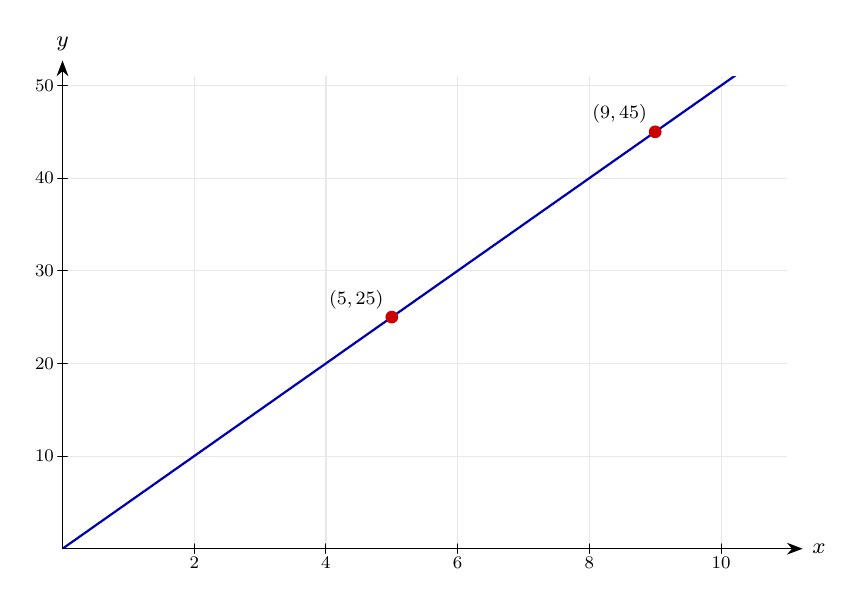
\begin{tikzpicture}[>={Stealth[length=2mm]},font=\footnotesize,line cap=round,line join=round]
\begin{scope}
\clip (0,0) rectangle (9.2,6);
\draw[gray!18] (0,0) grid[xstep=1.673,ystep=1.176] (9.2,6);
\draw[blue!70!black,thick] (0,0) -- (0.046,0.032) -- (0.092,0.065) -- (0.138,0.097) -- (0.184,0.129) -- (0.23,0.162) -- (0.276,0.194) -- (0.322,0.226) -- (0.368,0.259) -- (0.414,0.291) -- (0.46,0.324) -- (0.506,0.356) -- (0.552,0.388) -- (0.598,0.421) -- (0.644,0.453) -- (0.69,0.485) -- (0.736,0.518) -- (0.782,0.55) -- (0.828,0.582) -- (0.874,0.615) -- (0.92,0.647) -- (0.966,0.679) -- (1.012,0.712) -- (1.058,0.744) -- (1.104,0.776) -- (1.15,0.809) -- (1.196,0.841) -- (1.242,0.874) -- (1.288,0.906) -- (1.334,0.938) -- (1.38,0.971) -- (1.426,1.003) -- (1.472,1.035) -- (1.518,1.068) -- (1.564,1.1) -- (1.61,1.132) -- (1.656,1.165) -- (1.702,1.197) -- (1.748,1.229) -- (1.794,1.262) -- (1.84,1.294) -- (1.886,1.326) -- (1.932,1.359) -- (1.978,1.391) -- (2.024,1.424) -- (2.07,1.456) -- (2.116,1.488) -- (2.162,1.521) -- (2.208,1.553) -- (2.254,1.585) -- (2.3,1.618) -- (2.346,1.65) -- (2.392,1.682) -- (2.438,1.715) -- (2.484,1.747) -- (2.53,1.779) -- (2.576,1.812) -- (2.622,1.844) -- (2.668,1.876) -- (2.714,1.909) -- (2.76,1.941) -- (2.806,1.974) -- (2.852,2.006) -- (2.898,2.038) -- (2.944,2.071) -- (2.99,2.103) -- (3.036,2.135) -- (3.082,2.168) -- (3.128,2.2) -- (3.174,2.232) -- (3.22,2.265) -- (3.266,2.297) -- (3.312,2.329) -- (3.358,2.362) -- (3.404,2.394) -- (3.45,2.426) -- (3.496,2.459) -- (3.542,2.491) -- (3.588,2.524) -- (3.634,2.556) -- (3.68,2.588) -- (3.726,2.621) -- (3.772,2.653) -- (3.818,2.685) -- (3.864,2.718) -- (3.91,2.75) -- (3.956,2.782) -- (4.002,2.815) -- (4.048,2.847) -- (4.094,2.879) -- (4.14,2.912) -- (4.186,2.944) -- (4.232,2.976) -- (4.278,3.009) -- (4.324,3.041) -- (4.37,3.074) -- (4.416,3.106) -- (4.462,3.138) -- (4.508,3.171) -- (4.554,3.203) -- (4.6,3.235) -- (4.646,3.268) -- (4.692,3.3) -- (4.738,3.332) -- (4.784,3.365) -- (4.83,3.397) -- (4.876,3.429) -- (4.922,3.462) -- (4.968,3.494) -- (5.014,3.526) -- (5.06,3.559) -- (5.106,3.591) -- (5.152,3.624) -- (5.198,3.656) -- (5.244,3.688) -- (5.29,3.721) -- (5.336,3.753) -- (5.382,3.785) -- (5.428,3.818) -- (5.474,3.85) -- (5.52,3.882) -- (5.566,3.915) -- (5.612,3.947) -- (5.658,3.979) -- (5.704,4.012) -- (5.75,4.044) -- (5.796,4.076) -- (5.842,4.109) -- (5.888,4.141) -- (5.934,4.174) -- (5.98,4.206) -- (6.026,4.238) -- (6.072,4.271) -- (6.118,4.303) -- (6.164,4.335) -- (6.21,4.368) -- (6.256,4.4) -- (6.302,4.432) -- (6.348,4.465) -- (6.394,4.497) -- (6.44,4.529) -- (6.486,4.562) -- (6.532,4.594) -- (6.578,4.626) -- (6.624,4.659) -- (6.67,4.691) -- (6.716,4.724) -- (6.762,4.756) -- (6.808,4.788) -- (6.854,4.821) -- (6.9,4.853) -- (6.946,4.885) -- (6.992,4.918) -- (7.038,4.95) -- (7.084,4.982) -- (7.13,5.015) -- (7.176,5.047) -- (7.222,5.079) -- (7.268,5.112) -- (7.314,5.144) -- (7.36,5.176) -- (7.406,5.209) -- (7.452,5.241) -- (7.498,5.274) -- (7.544,5.306) -- (7.59,5.338) -- (7.636,5.371) -- (7.682,5.403) -- (7.728,5.435) -- (7.774,5.468) -- (7.82,5.5) -- (7.866,5.532) -- (7.912,5.565) -- (7.958,5.597) -- (8.004,5.629) -- (8.05,5.662) -- (8.096,5.694) -- (8.142,5.726) -- (8.188,5.759) -- (8.234,5.791) -- (8.28,5.824) -- (8.326,5.856) -- (8.372,5.888) -- (8.418,5.921) -- (8.464,5.953) -- (8.51,5.985) -- (8.556,6.018) -- (8.602,6.05) -- (8.648,6.082) -- (8.694,6.115) -- (8.74,6.147) -- (8.786,6.179) -- (8.832,6.212) -- (8.878,6.244) -- (8.924,6.276) -- (8.97,6.309) -- (9.016,6.341) -- (9.062,6.374) -- (9.108,6.406) -- (9.154,6.438) -- (9.2,6.471);
\end{scope}
\draw[->] (0,0) -- (9.4,0) node[right]{$x$};
\draw[->] (0,0) -- (0,6.2) node[above]{$y$};
\draw (1.673,-0.06) -- (1.673,0.06) node[below=2pt,scale=0.8]{$2$};
\draw (3.345,-0.06) -- (3.345,0.06) node[below=2pt,scale=0.8]{$4$};
\draw (5.018,-0.06) -- (5.018,0.06) node[below=2pt,scale=0.8]{$6$};
\draw (6.691,-0.06) -- (6.691,0.06) node[below=2pt,scale=0.8]{$8$};
\draw (8.364,-0.06) -- (8.364,0.06) node[below=2pt,scale=0.8]{$10$};
\draw (-0.06,1.176) -- (0.06,1.176) node[left=2pt,scale=0.8]{$10$};
\draw (-0.06,2.353) -- (0.06,2.353) node[left=2pt,scale=0.8]{$20$};
\draw (-0.06,3.529) -- (0.06,3.529) node[left=2pt,scale=0.8]{$30$};
\draw (-0.06,4.706) -- (0.06,4.706) node[left=2pt,scale=0.8]{$40$};
\draw (-0.06,5.882) -- (0.06,5.882) node[left=2pt,scale=0.8]{$50$};
\fill[red!80!black] (7.527,5.294) circle (2.3pt);
\node[above left,scale=0.85] at (7.527,5.294) {$(9,45)$};
\fill[red!80!black] (4.182,2.941) circle (2.3pt);
\node[above left,scale=0.85] at (4.182,2.941) {$(5,25)$};
\end{tikzpicture}
}
\end{center}
\small The relationship plotted, with the data points marked.\normalsize

\medskip\hrule

\section*{Proportion 02\quad\small\texttt{(cg4-002)}}
\addcontentsline{toc}{section}{Proportion 02 (cg4-002)}
\textit{Difficulty: Foundation \quad\textbar\quad Marks: 3}

\question{Given that \( y \propto x \) and that \( y = 36 \) when \( x = 4 \), find the value of \( x \) when \( y = 63 \).}

\textbf{Worked solution.}

\textit{Step 1: Write \( y = kx \) and substitute the known pair.}
\[\begin{gathered}
36 = k \times 4 \implies k = 9
\end{gathered}\]
The constant of proportionality is 9.

\textit{Step 2: Form the equation.}
\[\begin{gathered}
y = 9x
\end{gathered}\]
Now we can use any value of \( x \) or \( y \).

\textit{Step 3: Substitute \( y = 63 \) and solve for \( x \).}
\[\begin{gathered}
63 = 9x \implies x = 7
\end{gathered}\]
Divide both sides by 9.

\begin{answerbox}
\textbf{Final answer:}\quad \(\displaystyle  x = 7 \)
\end{answerbox}
\textbf{Graph.}

\begin{center}
\resizebox{\ifdim\width>\linewidth \linewidth\else \width\fi}{!}{%
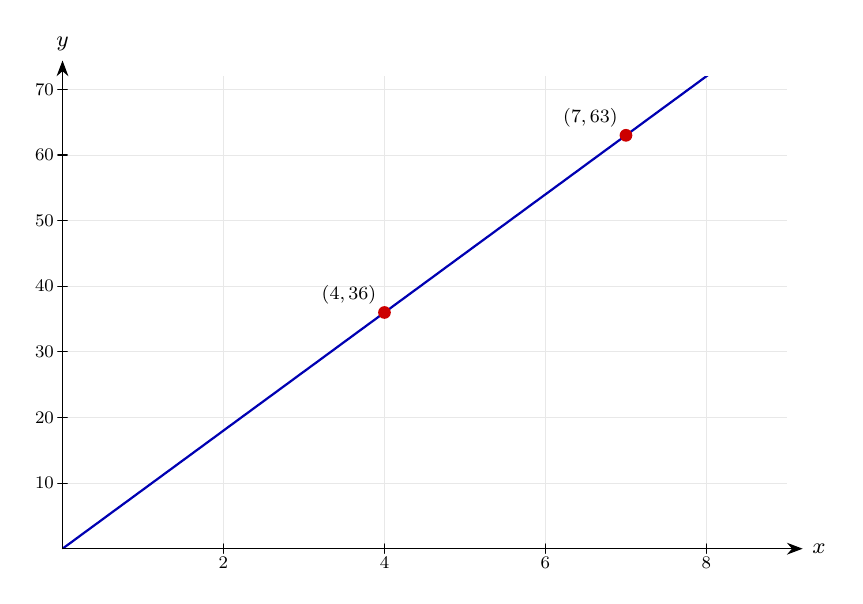
\begin{tikzpicture}[>={Stealth[length=2mm]},font=\footnotesize,line cap=round,line join=round]
\begin{scope}
\clip (0,0) rectangle (9.2,6);
\draw[gray!18] (0,0) grid[xstep=2.044,ystep=0.833] (9.2,6);
\draw[blue!70!black,thick] (0,0) -- (0.046,0.034) -- (0.092,0.067) -- (0.138,0.101) -- (0.184,0.135) -- (0.23,0.169) -- (0.276,0.203) -- (0.322,0.236) -- (0.368,0.27) -- (0.414,0.304) -- (0.46,0.337) -- (0.506,0.371) -- (0.552,0.405) -- (0.598,0.439) -- (0.644,0.473) -- (0.69,0.506) -- (0.736,0.54) -- (0.782,0.574) -- (0.828,0.607) -- (0.874,0.641) -- (0.92,0.675) -- (0.966,0.709) -- (1.012,0.742) -- (1.058,0.776) -- (1.104,0.81) -- (1.15,0.844) -- (1.196,0.877) -- (1.242,0.911) -- (1.288,0.945) -- (1.334,0.979) -- (1.38,1.012) -- (1.426,1.046) -- (1.472,1.08) -- (1.518,1.114) -- (1.564,1.147) -- (1.61,1.181) -- (1.656,1.215) -- (1.702,1.249) -- (1.748,1.282) -- (1.794,1.316) -- (1.84,1.35) -- (1.886,1.384) -- (1.932,1.417) -- (1.978,1.451) -- (2.024,1.485) -- (2.07,1.519) -- (2.116,1.553) -- (2.162,1.586) -- (2.208,1.62) -- (2.254,1.654) -- (2.3,1.688) -- (2.346,1.721) -- (2.392,1.755) -- (2.438,1.789) -- (2.484,1.823) -- (2.53,1.856) -- (2.576,1.89) -- (2.622,1.924) -- (2.668,1.957) -- (2.714,1.991) -- (2.76,2.025) -- (2.806,2.059) -- (2.852,2.092) -- (2.898,2.126) -- (2.944,2.16) -- (2.99,2.194) -- (3.036,2.228) -- (3.082,2.261) -- (3.128,2.295) -- (3.174,2.329) -- (3.22,2.362) -- (3.266,2.396) -- (3.312,2.43) -- (3.358,2.464) -- (3.404,2.497) -- (3.45,2.531) -- (3.496,2.565) -- (3.542,2.599) -- (3.588,2.633) -- (3.634,2.666) -- (3.68,2.7) -- (3.726,2.734) -- (3.772,2.768) -- (3.818,2.801) -- (3.864,2.835) -- (3.91,2.869) -- (3.956,2.902) -- (4.002,2.936) -- (4.048,2.97) -- (4.094,3.004) -- (4.14,3.037) -- (4.186,3.071) -- (4.232,3.105) -- (4.278,3.139) -- (4.324,3.172) -- (4.37,3.206) -- (4.416,3.24) -- (4.462,3.274) -- (4.508,3.307) -- (4.554,3.341) -- (4.6,3.375) -- (4.646,3.409) -- (4.692,3.442) -- (4.738,3.476) -- (4.784,3.51) -- (4.83,3.544) -- (4.876,3.578) -- (4.922,3.611) -- (4.968,3.645) -- (5.014,3.679) -- (5.06,3.713) -- (5.106,3.746) -- (5.152,3.78) -- (5.198,3.814) -- (5.244,3.848) -- (5.29,3.881) -- (5.336,3.915) -- (5.382,3.949) -- (5.428,3.982) -- (5.474,4.016) -- (5.52,4.05) -- (5.566,4.084) -- (5.612,4.117) -- (5.658,4.151) -- (5.704,4.185) -- (5.75,4.219) -- (5.796,4.252) -- (5.842,4.286) -- (5.888,4.32) -- (5.934,4.354) -- (5.98,4.388) -- (6.026,4.421) -- (6.072,4.455) -- (6.118,4.489) -- (6.164,4.522) -- (6.21,4.556) -- (6.256,4.59) -- (6.302,4.624) -- (6.348,4.657) -- (6.394,4.691) -- (6.44,4.725) -- (6.486,4.759) -- (6.532,4.792) -- (6.578,4.826) -- (6.624,4.86) -- (6.67,4.894) -- (6.716,4.928) -- (6.762,4.961) -- (6.808,4.995) -- (6.854,5.029) -- (6.9,5.063) -- (6.946,5.096) -- (6.992,5.13) -- (7.038,5.164) -- (7.084,5.197) -- (7.13,5.231) -- (7.176,5.265) -- (7.222,5.299) -- (7.268,5.332) -- (7.314,5.366) -- (7.36,5.4) -- (7.406,5.434) -- (7.452,5.468) -- (7.498,5.501) -- (7.544,5.535) -- (7.59,5.569) -- (7.636,5.603) -- (7.682,5.636) -- (7.728,5.67) -- (7.774,5.704) -- (7.82,5.737) -- (7.866,5.771) -- (7.912,5.805) -- (7.958,5.839) -- (8.004,5.872) -- (8.05,5.906) -- (8.096,5.94) -- (8.142,5.974) -- (8.188,6.008) -- (8.234,6.041) -- (8.28,6.075) -- (8.326,6.109) -- (8.372,6.142) -- (8.418,6.176) -- (8.464,6.21) -- (8.51,6.244) -- (8.556,6.278) -- (8.602,6.311) -- (8.648,6.345) -- (8.694,6.379) -- (8.74,6.412) -- (8.786,6.446) -- (8.832,6.48) -- (8.878,6.514) -- (8.924,6.548) -- (8.97,6.581) -- (9.016,6.615) -- (9.062,6.649) -- (9.108,6.682) -- (9.154,6.716) -- (9.2,6.75);
\end{scope}
\draw[->] (0,0) -- (9.4,0) node[right]{$x$};
\draw[->] (0,0) -- (0,6.2) node[above]{$y$};
\draw (2.044,-0.06) -- (2.044,0.06) node[below=2pt,scale=0.8]{$2$};
\draw (4.089,-0.06) -- (4.089,0.06) node[below=2pt,scale=0.8]{$4$};
\draw (6.133,-0.06) -- (6.133,0.06) node[below=2pt,scale=0.8]{$6$};
\draw (8.178,-0.06) -- (8.178,0.06) node[below=2pt,scale=0.8]{$8$};
\draw (-0.06,0.833) -- (0.06,0.833) node[left=2pt,scale=0.8]{$10$};
\draw (-0.06,1.667) -- (0.06,1.667) node[left=2pt,scale=0.8]{$20$};
\draw (-0.06,2.5) -- (0.06,2.5) node[left=2pt,scale=0.8]{$30$};
\draw (-0.06,3.333) -- (0.06,3.333) node[left=2pt,scale=0.8]{$40$};
\draw (-0.06,4.167) -- (0.06,4.167) node[left=2pt,scale=0.8]{$50$};
\draw (-0.06,5) -- (0.06,5) node[left=2pt,scale=0.8]{$60$};
\draw (-0.06,5.833) -- (0.06,5.833) node[left=2pt,scale=0.8]{$70$};
\fill[red!80!black] (4.089,3) circle (2.3pt);
\node[above left,scale=0.85] at (4.089,3) {$(4,36)$};
\fill[red!80!black] (7.156,5.25) circle (2.3pt);
\node[above left,scale=0.85] at (7.156,5.25) {$(7,63)$};
\end{tikzpicture}
}
\end{center}
\small The relationship plotted, with the data points marked.\normalsize

\medskip\hrule

\section*{Proportion 03\quad\small\texttt{(cg4-003)}}
\addcontentsline{toc}{section}{Proportion 03 (cg4-003)}
\textit{Difficulty: Foundation \quad\textbar\quad Marks: 3}

\question{A car uses petrol directly proportional to the distance it travels. It uses 6 litres to travel 48 km. How many litres does it use to travel 200 km?}

\textbf{Worked solution.}

\textit{Step 1: Let \( P \) litres of petrol and \( d \) km distance. Write \( P = kd \).}
\[\begin{gathered}
6 = k \times 48 \implies k = \frac{6}{48} = \frac{1}{8}
\end{gathered}\]
Find the constant of proportionality.

\textit{Step 2: Write the equation.}
\[\begin{gathered}
P = \frac{1}{8}\,d
\end{gathered}\]
The car uses 1 litre per 8 km.

\textit{Step 3: Substitute \( d = 200 \).}
\[\begin{gathered}
P = \frac{200}{8} = 25 \text{ litres}
\end{gathered}\]
Multiply the distance by the rate.

\begin{answerbox}
\textbf{Final answer:}\quad \(\displaystyle  25 \) litres
\end{answerbox}
\textbf{Graph.}

\begin{center}
\resizebox{\ifdim\width>\linewidth \linewidth\else \width\fi}{!}{%
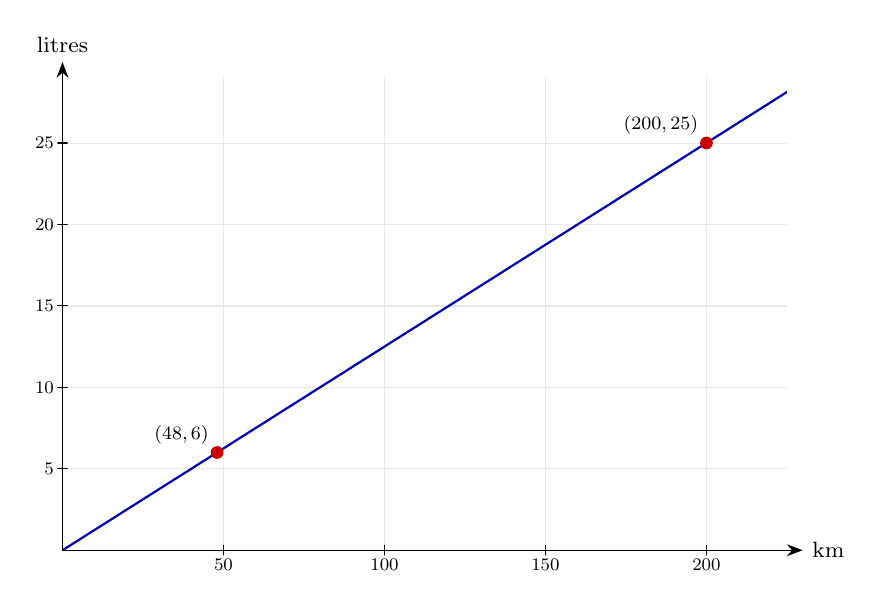
\begin{tikzpicture}[>={Stealth[length=2mm]},font=\footnotesize,line cap=round,line join=round]
\begin{scope}
\clip (0,0) rectangle (9.2,6);
\draw[gray!18] (0,0) grid[xstep=2.044,ystep=1.034] (9.2,6);
\draw[blue!70!black,thick] (0,0) -- (0.046,0.029) -- (0.092,0.058) -- (0.138,0.087) -- (0.184,0.116) -- (0.23,0.145) -- (0.276,0.175) -- (0.322,0.204) -- (0.368,0.233) -- (0.414,0.262) -- (0.46,0.291) -- (0.506,0.32) -- (0.552,0.349) -- (0.598,0.378) -- (0.644,0.407) -- (0.69,0.436) -- (0.736,0.466) -- (0.782,0.495) -- (0.828,0.524) -- (0.874,0.553) -- (0.92,0.582) -- (0.966,0.611) -- (1.012,0.64) -- (1.058,0.669) -- (1.104,0.698) -- (1.15,0.727) -- (1.196,0.756) -- (1.242,0.786) -- (1.288,0.815) -- (1.334,0.844) -- (1.38,0.873) -- (1.426,0.902) -- (1.472,0.931) -- (1.518,0.96) -- (1.564,0.989) -- (1.61,1.018) -- (1.656,1.047) -- (1.702,1.077) -- (1.748,1.106) -- (1.794,1.135) -- (1.84,1.164) -- (1.886,1.193) -- (1.932,1.222) -- (1.978,1.251) -- (2.024,1.28) -- (2.07,1.309) -- (2.116,1.338) -- (2.162,1.367) -- (2.208,1.397) -- (2.254,1.426) -- (2.3,1.455) -- (2.346,1.484) -- (2.392,1.513) -- (2.438,1.542) -- (2.484,1.571) -- (2.53,1.6) -- (2.576,1.629) -- (2.622,1.658) -- (2.668,1.688) -- (2.714,1.717) -- (2.76,1.746) -- (2.806,1.775) -- (2.852,1.804) -- (2.898,1.833) -- (2.944,1.862) -- (2.99,1.891) -- (3.036,1.92) -- (3.082,1.949) -- (3.128,1.978) -- (3.174,2.008) -- (3.22,2.037) -- (3.266,2.066) -- (3.312,2.095) -- (3.358,2.124) -- (3.404,2.153) -- (3.45,2.182) -- (3.496,2.211) -- (3.542,2.24) -- (3.588,2.269) -- (3.634,2.298) -- (3.68,2.328) -- (3.726,2.357) -- (3.772,2.386) -- (3.818,2.415) -- (3.864,2.444) -- (3.91,2.473) -- (3.956,2.502) -- (4.002,2.531) -- (4.048,2.56) -- (4.094,2.589) -- (4.14,2.619) -- (4.186,2.648) -- (4.232,2.677) -- (4.278,2.706) -- (4.324,2.735) -- (4.37,2.764) -- (4.416,2.793) -- (4.462,2.822) -- (4.508,2.851) -- (4.554,2.88) -- (4.6,2.909) -- (4.646,2.939) -- (4.692,2.968) -- (4.738,2.997) -- (4.784,3.026) -- (4.83,3.055) -- (4.876,3.084) -- (4.922,3.113) -- (4.968,3.142) -- (5.014,3.171) -- (5.06,3.2) -- (5.106,3.23) -- (5.152,3.259) -- (5.198,3.288) -- (5.244,3.317) -- (5.29,3.346) -- (5.336,3.375) -- (5.382,3.404) -- (5.428,3.433) -- (5.474,3.462) -- (5.52,3.491) -- (5.566,3.52) -- (5.612,3.55) -- (5.658,3.579) -- (5.704,3.608) -- (5.75,3.637) -- (5.796,3.666) -- (5.842,3.695) -- (5.888,3.724) -- (5.934,3.753) -- (5.98,3.782) -- (6.026,3.811) -- (6.072,3.841) -- (6.118,3.87) -- (6.164,3.899) -- (6.21,3.928) -- (6.256,3.957) -- (6.302,3.986) -- (6.348,4.015) -- (6.394,4.044) -- (6.44,4.073) -- (6.486,4.102) -- (6.532,4.131) -- (6.578,4.161) -- (6.624,4.19) -- (6.67,4.219) -- (6.716,4.248) -- (6.762,4.277) -- (6.808,4.306) -- (6.854,4.335) -- (6.9,4.364) -- (6.946,4.393) -- (6.992,4.422) -- (7.038,4.452) -- (7.084,4.481) -- (7.13,4.51) -- (7.176,4.539) -- (7.222,4.568) -- (7.268,4.597) -- (7.314,4.626) -- (7.36,4.655) -- (7.406,4.684) -- (7.452,4.713) -- (7.498,4.742) -- (7.544,4.772) -- (7.59,4.801) -- (7.636,4.83) -- (7.682,4.859) -- (7.728,4.888) -- (7.774,4.917) -- (7.82,4.946) -- (7.866,4.975) -- (7.912,5.004) -- (7.958,5.033) -- (8.004,5.063) -- (8.05,5.092) -- (8.096,5.121) -- (8.142,5.15) -- (8.188,5.179) -- (8.234,5.208) -- (8.28,5.237) -- (8.326,5.266) -- (8.372,5.295) -- (8.418,5.324) -- (8.464,5.353) -- (8.51,5.383) -- (8.556,5.412) -- (8.602,5.441) -- (8.648,5.47) -- (8.694,5.499) -- (8.74,5.528) -- (8.786,5.557) -- (8.832,5.586) -- (8.878,5.615) -- (8.924,5.644) -- (8.97,5.673) -- (9.016,5.703) -- (9.062,5.732) -- (9.108,5.761) -- (9.154,5.79) -- (9.2,5.819);
\end{scope}
\draw[->] (0,0) -- (9.4,0) node[right]{$\text{km}$};
\draw[->] (0,0) -- (0,6.2) node[above]{$\text{litres}$};
\draw (2.044,-0.06) -- (2.044,0.06) node[below=2pt,scale=0.8]{$50$};
\draw (4.089,-0.06) -- (4.089,0.06) node[below=2pt,scale=0.8]{$100$};
\draw (6.133,-0.06) -- (6.133,0.06) node[below=2pt,scale=0.8]{$150$};
\draw (8.178,-0.06) -- (8.178,0.06) node[below=2pt,scale=0.8]{$200$};
\draw (-0.06,1.034) -- (0.06,1.034) node[left=2pt,scale=0.8]{$5$};
\draw (-0.06,2.069) -- (0.06,2.069) node[left=2pt,scale=0.8]{$10$};
\draw (-0.06,3.103) -- (0.06,3.103) node[left=2pt,scale=0.8]{$15$};
\draw (-0.06,4.138) -- (0.06,4.138) node[left=2pt,scale=0.8]{$20$};
\draw (-0.06,5.172) -- (0.06,5.172) node[left=2pt,scale=0.8]{$25$};
\fill[red!80!black] (1.963,1.241) circle (2.3pt);
\node[above left,scale=0.85] at (1.963,1.241) {$(48,6)$};
\fill[red!80!black] (8.178,5.172) circle (2.3pt);
\node[above left,scale=0.85] at (8.178,5.172) {$(200,25)$};
\end{tikzpicture}
}
\end{center}
\small The relationship plotted, with the data points marked.\normalsize

\medskip\hrule

\section*{Proportion 04\quad\small\texttt{(cg4-004)}}
\addcontentsline{toc}{section}{Proportion 04 (cg4-004)}
\textit{Difficulty: Foundation \quad\textbar\quad Marks: 4}

\question{Given that \( y \propto x \), that \( y = 15 \) when \( x = a \), and that \( y = a \) when \( x = 60 \), find the positive value of \( a \).}

\textbf{Worked solution.}

\textit{Step 1: Write \( y = kx \) and use the first pair.}
\[\begin{gathered}
15 = ka \implies k = \frac{15}{a}
\end{gathered}\]
Express \( k \) in terms of \( a \).

\textit{Step 2: Substitute the second pair \( y = a,\, x = 60 \).}
\[\begin{gathered}
a = k \times 60 = \frac{15}{a} \times 60 = \frac{900}{a}
\end{gathered}\]
Replace \( k \) with the expression found above.

\textit{Step 3: Solve \( a^2 = 900 \).}
\[\begin{gathered}
a^2 = 900 \implies a = 30 \quad (a > 0)
\end{gathered}\]
Take the positive square root.

\begin{answerbox}
\textbf{Final answer:}\quad \(\displaystyle  a = 30 \)
\end{answerbox}
\textbf{Graph.}

\begin{center}
\resizebox{\ifdim\width>\linewidth \linewidth\else \width\fi}{!}{%
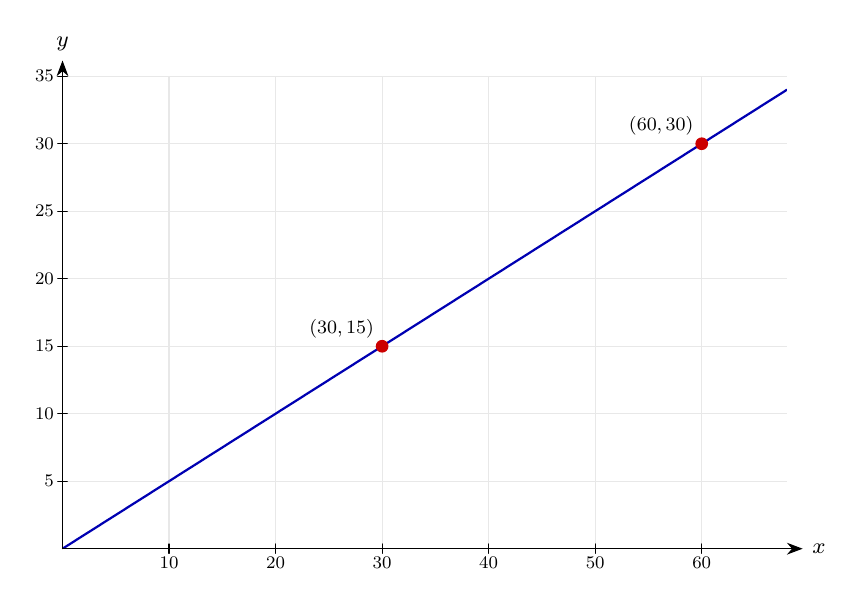
\begin{tikzpicture}[>={Stealth[length=2mm]},font=\footnotesize,line cap=round,line join=round]
\begin{scope}
\clip (0,0) rectangle (9.2,6);
\draw[gray!18] (0,0) grid[xstep=1.353,ystep=0.857] (9.2,6);
\draw[blue!70!black,thick] (0,0) -- (0.046,0.029) -- (0.092,0.058) -- (0.138,0.087) -- (0.184,0.117) -- (0.23,0.146) -- (0.276,0.175) -- (0.322,0.204) -- (0.368,0.233) -- (0.414,0.262) -- (0.46,0.291) -- (0.506,0.321) -- (0.552,0.35) -- (0.598,0.379) -- (0.644,0.408) -- (0.69,0.437) -- (0.736,0.466) -- (0.782,0.495) -- (0.828,0.525) -- (0.874,0.554) -- (0.92,0.583) -- (0.966,0.612) -- (1.012,0.641) -- (1.058,0.67) -- (1.104,0.699) -- (1.15,0.729) -- (1.196,0.758) -- (1.242,0.787) -- (1.288,0.816) -- (1.334,0.845) -- (1.38,0.874) -- (1.426,0.903) -- (1.472,0.933) -- (1.518,0.962) -- (1.564,0.991) -- (1.61,1.02) -- (1.656,1.049) -- (1.702,1.078) -- (1.748,1.107) -- (1.794,1.137) -- (1.84,1.166) -- (1.886,1.195) -- (1.932,1.224) -- (1.978,1.253) -- (2.024,1.282) -- (2.07,1.311) -- (2.116,1.341) -- (2.162,1.37) -- (2.208,1.399) -- (2.254,1.428) -- (2.3,1.457) -- (2.346,1.486) -- (2.392,1.515) -- (2.438,1.545) -- (2.484,1.574) -- (2.53,1.603) -- (2.576,1.632) -- (2.622,1.661) -- (2.668,1.69) -- (2.714,1.719) -- (2.76,1.749) -- (2.806,1.778) -- (2.852,1.807) -- (2.898,1.836) -- (2.944,1.865) -- (2.99,1.894) -- (3.036,1.923) -- (3.082,1.953) -- (3.128,1.982) -- (3.174,2.011) -- (3.22,2.04) -- (3.266,2.069) -- (3.312,2.098) -- (3.358,2.127) -- (3.404,2.157) -- (3.45,2.186) -- (3.496,2.215) -- (3.542,2.244) -- (3.588,2.273) -- (3.634,2.302) -- (3.68,2.331) -- (3.726,2.361) -- (3.772,2.39) -- (3.818,2.419) -- (3.864,2.448) -- (3.91,2.477) -- (3.956,2.506) -- (4.002,2.535) -- (4.048,2.565) -- (4.094,2.594) -- (4.14,2.623) -- (4.186,2.652) -- (4.232,2.681) -- (4.278,2.71) -- (4.324,2.739) -- (4.37,2.769) -- (4.416,2.798) -- (4.462,2.827) -- (4.508,2.856) -- (4.554,2.885) -- (4.6,2.914) -- (4.646,2.943) -- (4.692,2.973) -- (4.738,3.002) -- (4.784,3.031) -- (4.83,3.06) -- (4.876,3.089) -- (4.922,3.118) -- (4.968,3.147) -- (5.014,3.177) -- (5.06,3.206) -- (5.106,3.235) -- (5.152,3.264) -- (5.198,3.293) -- (5.244,3.322) -- (5.29,3.351) -- (5.336,3.381) -- (5.382,3.41) -- (5.428,3.439) -- (5.474,3.468) -- (5.52,3.497) -- (5.566,3.526) -- (5.612,3.555) -- (5.658,3.585) -- (5.704,3.614) -- (5.75,3.643) -- (5.796,3.672) -- (5.842,3.701) -- (5.888,3.73) -- (5.934,3.759) -- (5.98,3.789) -- (6.026,3.818) -- (6.072,3.847) -- (6.118,3.876) -- (6.164,3.905) -- (6.21,3.934) -- (6.256,3.963) -- (6.302,3.993) -- (6.348,4.022) -- (6.394,4.051) -- (6.44,4.08) -- (6.486,4.109) -- (6.532,4.138) -- (6.578,4.167) -- (6.624,4.197) -- (6.67,4.226) -- (6.716,4.255) -- (6.762,4.284) -- (6.808,4.313) -- (6.854,4.342) -- (6.9,4.371) -- (6.946,4.401) -- (6.992,4.43) -- (7.038,4.459) -- (7.084,4.488) -- (7.13,4.517) -- (7.176,4.546) -- (7.222,4.575) -- (7.268,4.605) -- (7.314,4.634) -- (7.36,4.663) -- (7.406,4.692) -- (7.452,4.721) -- (7.498,4.75) -- (7.544,4.779) -- (7.59,4.809) -- (7.636,4.838) -- (7.682,4.867) -- (7.728,4.896) -- (7.774,4.925) -- (7.82,4.954) -- (7.866,4.983) -- (7.912,5.013) -- (7.958,5.042) -- (8.004,5.071) -- (8.05,5.1) -- (8.096,5.129) -- (8.142,5.158) -- (8.188,5.187) -- (8.234,5.217) -- (8.28,5.246) -- (8.326,5.275) -- (8.372,5.304) -- (8.418,5.333) -- (8.464,5.362) -- (8.51,5.391) -- (8.556,5.421) -- (8.602,5.45) -- (8.648,5.479) -- (8.694,5.508) -- (8.74,5.537) -- (8.786,5.566) -- (8.832,5.595) -- (8.878,5.625) -- (8.924,5.654) -- (8.97,5.683) -- (9.016,5.712) -- (9.062,5.741) -- (9.108,5.77) -- (9.154,5.799) -- (9.2,5.829);
\end{scope}
\draw[->] (0,0) -- (9.4,0) node[right]{$x$};
\draw[->] (0,0) -- (0,6.2) node[above]{$y$};
\draw (1.353,-0.06) -- (1.353,0.06) node[below=2pt,scale=0.8]{$10$};
\draw (2.706,-0.06) -- (2.706,0.06) node[below=2pt,scale=0.8]{$20$};
\draw (4.059,-0.06) -- (4.059,0.06) node[below=2pt,scale=0.8]{$30$};
\draw (5.412,-0.06) -- (5.412,0.06) node[below=2pt,scale=0.8]{$40$};
\draw (6.765,-0.06) -- (6.765,0.06) node[below=2pt,scale=0.8]{$50$};
\draw (8.118,-0.06) -- (8.118,0.06) node[below=2pt,scale=0.8]{$60$};
\draw (-0.06,0.857) -- (0.06,0.857) node[left=2pt,scale=0.8]{$5$};
\draw (-0.06,1.714) -- (0.06,1.714) node[left=2pt,scale=0.8]{$10$};
\draw (-0.06,2.571) -- (0.06,2.571) node[left=2pt,scale=0.8]{$15$};
\draw (-0.06,3.429) -- (0.06,3.429) node[left=2pt,scale=0.8]{$20$};
\draw (-0.06,4.286) -- (0.06,4.286) node[left=2pt,scale=0.8]{$25$};
\draw (-0.06,5.143) -- (0.06,5.143) node[left=2pt,scale=0.8]{$30$};
\draw (-0.06,6) -- (0.06,6) node[left=2pt,scale=0.8]{$35$};
\fill[red!80!black] (4.059,2.571) circle (2.3pt);
\node[above left,scale=0.85] at (4.059,2.571) {$(30,15)$};
\fill[red!80!black] (8.118,5.143) circle (2.3pt);
\node[above left,scale=0.85] at (8.118,5.143) {$(60,30)$};
\end{tikzpicture}
}
\end{center}
\small The relationship plotted, with the data points marked.\normalsize

\medskip\hrule

\section*{Proportion 05\quad\small\texttt{(cg4-005)}}
\addcontentsline{toc}{section}{Proportion 05 (cg4-005)}
\textit{Difficulty: Foundation \quad\textbar\quad Marks: 3}

\question{A plumber charges a call-out fee of \pounds 0 plus an amount directly proportional to the number of hours worked. She charges \pounds 84 for 3 hours. How much does she charge for 7 hours?}

\textbf{Worked solution.}

\textit{Step 1: Let \( C \) = charge (\pounds ) and \( h \) = hours. Write \( C = kh \).}
\[\begin{gathered}
84 = k \times 3 \implies k = 28
\end{gathered}\]
She charges \pounds 28 per hour.

\textit{Step 2: Form the equation.}
\[\begin{gathered}
C = 28h
\end{gathered}\]
The constant of proportionality is 28.

\textit{Step 3: Substitute \( h = 7 \).}
\[\begin{gathered}
C = 28 \times 7 = \pounds 196
\end{gathered}\]
Multiply hours by the rate.

\begin{answerbox}
\textbf{Final answer:}\quad \(\displaystyle  \pounds 196 \)
\end{answerbox}
\textbf{Graph.}

\begin{center}
\resizebox{\ifdim\width>\linewidth \linewidth\else \width\fi}{!}{%
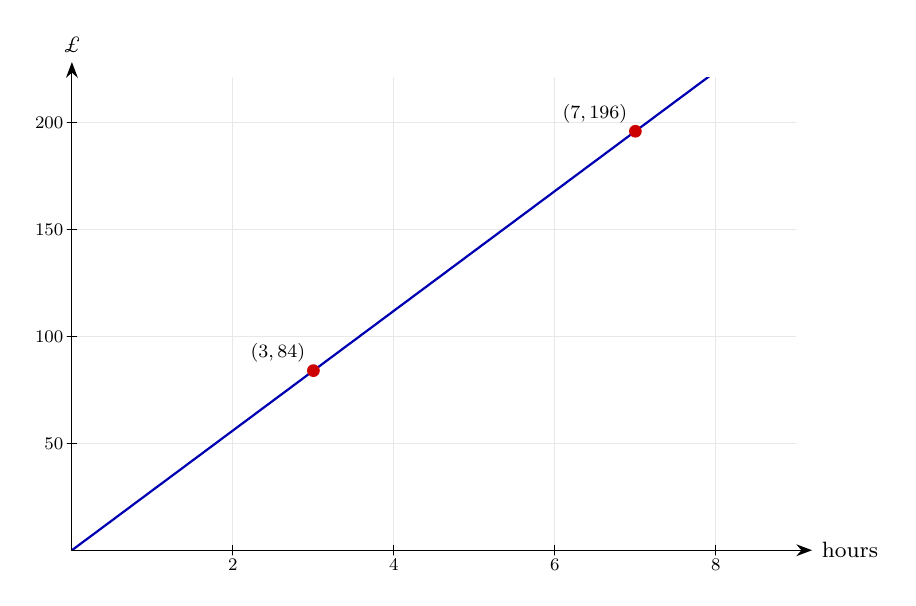
\begin{tikzpicture}[>={Stealth[length=2mm]},font=\footnotesize,line cap=round,line join=round]
\begin{scope}
\clip (0,0) rectangle (9.2,6);
\draw[gray!18] (0,0) grid[xstep=2.044,ystep=1.357] (9.2,6);
\draw[blue!70!black,thick] (0,0) -- (0.046,0.034) -- (0.092,0.068) -- (0.138,0.103) -- (0.184,0.137) -- (0.23,0.171) -- (0.276,0.205) -- (0.322,0.239) -- (0.368,0.274) -- (0.414,0.308) -- (0.46,0.342) -- (0.506,0.376) -- (0.552,0.41) -- (0.598,0.445) -- (0.644,0.479) -- (0.69,0.513) -- (0.736,0.547) -- (0.782,0.582) -- (0.828,0.616) -- (0.874,0.65) -- (0.92,0.684) -- (0.966,0.718) -- (1.012,0.753) -- (1.058,0.787) -- (1.104,0.821) -- (1.15,0.855) -- (1.196,0.889) -- (1.242,0.924) -- (1.288,0.958) -- (1.334,0.992) -- (1.38,1.026) -- (1.426,1.06) -- (1.472,1.095) -- (1.518,1.129) -- (1.564,1.163) -- (1.61,1.197) -- (1.656,1.231) -- (1.702,1.266) -- (1.748,1.3) -- (1.794,1.334) -- (1.84,1.368) -- (1.886,1.403) -- (1.932,1.437) -- (1.978,1.471) -- (2.024,1.505) -- (2.07,1.539) -- (2.116,1.574) -- (2.162,1.608) -- (2.208,1.642) -- (2.254,1.676) -- (2.3,1.71) -- (2.346,1.745) -- (2.392,1.779) -- (2.438,1.813) -- (2.484,1.847) -- (2.53,1.881) -- (2.576,1.916) -- (2.622,1.95) -- (2.668,1.984) -- (2.714,2.018) -- (2.76,2.052) -- (2.806,2.087) -- (2.852,2.121) -- (2.898,2.155) -- (2.944,2.189) -- (2.99,2.224) -- (3.036,2.258) -- (3.082,2.292) -- (3.128,2.326) -- (3.174,2.36) -- (3.22,2.395) -- (3.266,2.429) -- (3.312,2.463) -- (3.358,2.497) -- (3.404,2.531) -- (3.45,2.566) -- (3.496,2.6) -- (3.542,2.634) -- (3.588,2.668) -- (3.634,2.702) -- (3.68,2.737) -- (3.726,2.771) -- (3.772,2.805) -- (3.818,2.839) -- (3.864,2.873) -- (3.91,2.908) -- (3.956,2.942) -- (4.002,2.976) -- (4.048,3.01) -- (4.094,3.045) -- (4.14,3.079) -- (4.186,3.113) -- (4.232,3.147) -- (4.278,3.181) -- (4.324,3.216) -- (4.37,3.25) -- (4.416,3.284) -- (4.462,3.318) -- (4.508,3.352) -- (4.554,3.387) -- (4.6,3.421) -- (4.646,3.455) -- (4.692,3.489) -- (4.738,3.523) -- (4.784,3.558) -- (4.83,3.592) -- (4.876,3.626) -- (4.922,3.66) -- (4.968,3.694) -- (5.014,3.729) -- (5.06,3.763) -- (5.106,3.797) -- (5.152,3.831) -- (5.198,3.866) -- (5.244,3.9) -- (5.29,3.934) -- (5.336,3.968) -- (5.382,4.002) -- (5.428,4.037) -- (5.474,4.071) -- (5.52,4.105) -- (5.566,4.139) -- (5.612,4.173) -- (5.658,4.208) -- (5.704,4.242) -- (5.75,4.276) -- (5.796,4.31) -- (5.842,4.344) -- (5.888,4.379) -- (5.934,4.413) -- (5.98,4.447) -- (6.026,4.481) -- (6.072,4.515) -- (6.118,4.55) -- (6.164,4.584) -- (6.21,4.618) -- (6.256,4.652) -- (6.302,4.687) -- (6.348,4.721) -- (6.394,4.755) -- (6.44,4.789) -- (6.486,4.823) -- (6.532,4.858) -- (6.578,4.892) -- (6.624,4.926) -- (6.67,4.96) -- (6.716,4.994) -- (6.762,5.029) -- (6.808,5.063) -- (6.854,5.097) -- (6.9,5.131) -- (6.946,5.165) -- (6.992,5.2) -- (7.038,5.234) -- (7.084,5.268) -- (7.13,5.302) -- (7.176,5.336) -- (7.222,5.371) -- (7.268,5.405) -- (7.314,5.439) -- (7.36,5.473) -- (7.406,5.508) -- (7.452,5.542) -- (7.498,5.576) -- (7.544,5.61) -- (7.59,5.644) -- (7.636,5.679) -- (7.682,5.713) -- (7.728,5.747) -- (7.774,5.781) -- (7.82,5.815) -- (7.866,5.85) -- (7.912,5.884) -- (7.958,5.918) -- (8.004,5.952) -- (8.05,5.986) -- (8.096,6.021) -- (8.142,6.055) -- (8.188,6.089) -- (8.234,6.123) -- (8.28,6.157) -- (8.326,6.192) -- (8.372,6.226) -- (8.418,6.26) -- (8.464,6.294) -- (8.51,6.329) -- (8.556,6.363) -- (8.602,6.397) -- (8.648,6.431) -- (8.694,6.465) -- (8.74,6.5) -- (8.786,6.534) -- (8.832,6.568) -- (8.878,6.602) -- (8.924,6.636) -- (8.97,6.671) -- (9.016,6.705) -- (9.062,6.739) -- (9.108,6.773) -- (9.154,6.807) -- (9.2,6.842);
\end{scope}
\draw[->] (0,0) -- (9.4,0) node[right]{$\text{hours}$};
\draw[->] (0,0) -- (0,6.2) node[above]{$\pounds$};
\draw (2.044,-0.06) -- (2.044,0.06) node[below=2pt,scale=0.8]{$2$};
\draw (4.089,-0.06) -- (4.089,0.06) node[below=2pt,scale=0.8]{$4$};
\draw (6.133,-0.06) -- (6.133,0.06) node[below=2pt,scale=0.8]{$6$};
\draw (8.178,-0.06) -- (8.178,0.06) node[below=2pt,scale=0.8]{$8$};
\draw (-0.06,1.357) -- (0.06,1.357) node[left=2pt,scale=0.8]{$50$};
\draw (-0.06,2.715) -- (0.06,2.715) node[left=2pt,scale=0.8]{$100$};
\draw (-0.06,4.072) -- (0.06,4.072) node[left=2pt,scale=0.8]{$150$};
\draw (-0.06,5.43) -- (0.06,5.43) node[left=2pt,scale=0.8]{$200$};
\fill[red!80!black] (3.067,2.281) circle (2.3pt);
\node[above left,scale=0.85] at (3.067,2.281) {$(3,84)$};
\fill[red!80!black] (7.156,5.321) circle (2.3pt);
\node[above left,scale=0.85] at (7.156,5.321) {$(7,196)$};
\end{tikzpicture}
}
\end{center}
\small The relationship plotted, with the data points marked.\normalsize

\medskip\hrule

\section*{Proportion 06\quad\small\texttt{(cg4-006)}}
\addcontentsline{toc}{section}{Proportion 06 (cg4-006)}
\textit{Difficulty: Foundation \quad\textbar\quad Marks: 3}

\question{Given that \( y \propto x \), \( y = 30 \) when \( x = 12 \), and \( y = 75 \) when \( x = a \), find \( a \).}

\textbf{Worked solution.}

\textit{Step 1: Find \( k \) using the first known pair.}
\[\begin{gathered}
k = \frac{30}{12} = \frac{5}{2}
\end{gathered}\]
The constant of proportionality is \( \frac{5}{2} \).

\textit{Step 2: Use \( y = 75 \) to find \( a \).}
\[\begin{gathered}
75 = \frac{5}{2} \times a \implies a = \frac{75 \times 2}{5} = 30
\end{gathered}\]
Multiply both sides by \( \frac{2}{5} \).

\begin{answerbox}
\textbf{Final answer:}\quad \(\displaystyle  a = 30 \)
\end{answerbox}
\textbf{Graph.}

\begin{center}
\resizebox{\ifdim\width>\linewidth \linewidth\else \width\fi}{!}{%
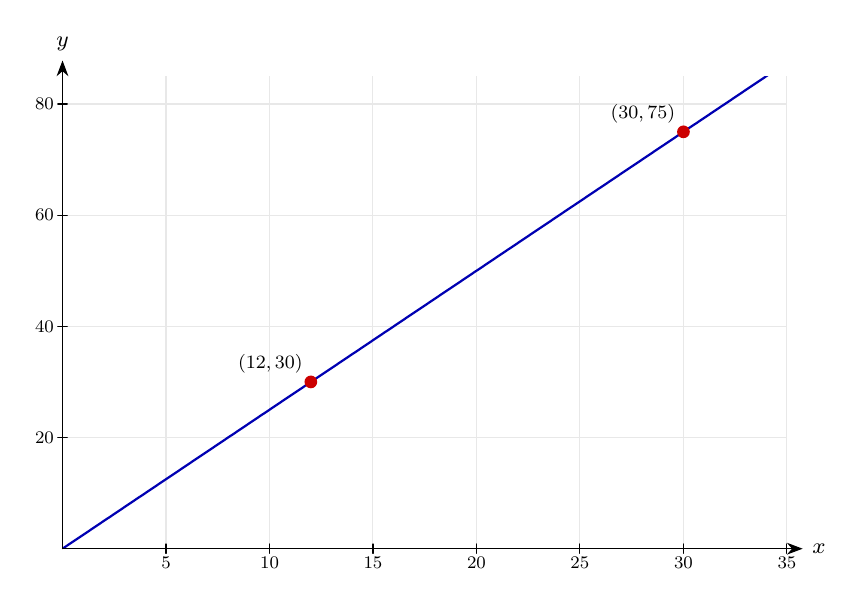
\begin{tikzpicture}[>={Stealth[length=2mm]},font=\footnotesize,line cap=round,line join=round]
\begin{scope}
\clip (0,0) rectangle (9.2,6);
\draw[gray!18] (0,0) grid[xstep=1.314,ystep=1.412] (9.2,6);
\draw[blue!70!black,thick] (0,0) -- (0.046,0.031) -- (0.092,0.062) -- (0.138,0.093) -- (0.184,0.124) -- (0.23,0.154) -- (0.276,0.185) -- (0.322,0.216) -- (0.368,0.247) -- (0.414,0.278) -- (0.46,0.309) -- (0.506,0.34) -- (0.552,0.371) -- (0.598,0.401) -- (0.644,0.432) -- (0.69,0.463) -- (0.736,0.494) -- (0.782,0.525) -- (0.828,0.556) -- (0.874,0.587) -- (0.92,0.618) -- (0.966,0.649) -- (1.012,0.679) -- (1.058,0.71) -- (1.104,0.741) -- (1.15,0.772) -- (1.196,0.803) -- (1.242,0.834) -- (1.288,0.865) -- (1.334,0.896) -- (1.38,0.926) -- (1.426,0.957) -- (1.472,0.988) -- (1.518,1.019) -- (1.564,1.05) -- (1.61,1.081) -- (1.656,1.112) -- (1.702,1.143) -- (1.748,1.174) -- (1.794,1.204) -- (1.84,1.235) -- (1.886,1.266) -- (1.932,1.297) -- (1.978,1.328) -- (2.024,1.359) -- (2.07,1.39) -- (2.116,1.421) -- (2.162,1.451) -- (2.208,1.482) -- (2.254,1.513) -- (2.3,1.544) -- (2.346,1.575) -- (2.392,1.606) -- (2.438,1.637) -- (2.484,1.668) -- (2.53,1.699) -- (2.576,1.729) -- (2.622,1.76) -- (2.668,1.791) -- (2.714,1.822) -- (2.76,1.853) -- (2.806,1.884) -- (2.852,1.915) -- (2.898,1.946) -- (2.944,1.976) -- (2.99,2.007) -- (3.036,2.038) -- (3.082,2.069) -- (3.128,2.1) -- (3.174,2.131) -- (3.22,2.162) -- (3.266,2.193) -- (3.312,2.224) -- (3.358,2.254) -- (3.404,2.285) -- (3.45,2.316) -- (3.496,2.347) -- (3.542,2.378) -- (3.588,2.409) -- (3.634,2.44) -- (3.68,2.471) -- (3.726,2.501) -- (3.772,2.532) -- (3.818,2.563) -- (3.864,2.594) -- (3.91,2.625) -- (3.956,2.656) -- (4.002,2.687) -- (4.048,2.718) -- (4.094,2.749) -- (4.14,2.779) -- (4.186,2.81) -- (4.232,2.841) -- (4.278,2.872) -- (4.324,2.903) -- (4.37,2.934) -- (4.416,2.965) -- (4.462,2.996) -- (4.508,3.026) -- (4.554,3.057) -- (4.6,3.088) -- (4.646,3.119) -- (4.692,3.15) -- (4.738,3.181) -- (4.784,3.212) -- (4.83,3.243) -- (4.876,3.274) -- (4.922,3.304) -- (4.968,3.335) -- (5.014,3.366) -- (5.06,3.397) -- (5.106,3.428) -- (5.152,3.459) -- (5.198,3.49) -- (5.244,3.521) -- (5.29,3.551) -- (5.336,3.582) -- (5.382,3.613) -- (5.428,3.644) -- (5.474,3.675) -- (5.52,3.706) -- (5.566,3.737) -- (5.612,3.768) -- (5.658,3.799) -- (5.704,3.829) -- (5.75,3.86) -- (5.796,3.891) -- (5.842,3.922) -- (5.888,3.953) -- (5.934,3.984) -- (5.98,4.015) -- (6.026,4.046) -- (6.072,4.076) -- (6.118,4.107) -- (6.164,4.138) -- (6.21,4.169) -- (6.256,4.2) -- (6.302,4.231) -- (6.348,4.262) -- (6.394,4.293) -- (6.44,4.324) -- (6.486,4.354) -- (6.532,4.385) -- (6.578,4.416) -- (6.624,4.447) -- (6.67,4.478) -- (6.716,4.509) -- (6.762,4.54) -- (6.808,4.571) -- (6.854,4.601) -- (6.9,4.632) -- (6.946,4.663) -- (6.992,4.694) -- (7.038,4.725) -- (7.084,4.756) -- (7.13,4.787) -- (7.176,4.818) -- (7.222,4.849) -- (7.268,4.879) -- (7.314,4.91) -- (7.36,4.941) -- (7.406,4.972) -- (7.452,5.003) -- (7.498,5.034) -- (7.544,5.065) -- (7.59,5.096) -- (7.636,5.126) -- (7.682,5.157) -- (7.728,5.188) -- (7.774,5.219) -- (7.82,5.25) -- (7.866,5.281) -- (7.912,5.312) -- (7.958,5.343) -- (8.004,5.374) -- (8.05,5.404) -- (8.096,5.435) -- (8.142,5.466) -- (8.188,5.497) -- (8.234,5.528) -- (8.28,5.559) -- (8.326,5.59) -- (8.372,5.621) -- (8.418,5.651) -- (8.464,5.682) -- (8.51,5.713) -- (8.556,5.744) -- (8.602,5.775) -- (8.648,5.806) -- (8.694,5.837) -- (8.74,5.868) -- (8.786,5.899) -- (8.832,5.929) -- (8.878,5.96) -- (8.924,5.991) -- (8.97,6.022) -- (9.016,6.053) -- (9.062,6.084) -- (9.108,6.115) -- (9.154,6.146) -- (9.2,6.176);
\end{scope}
\draw[->] (0,0) -- (9.4,0) node[right]{$x$};
\draw[->] (0,0) -- (0,6.2) node[above]{$y$};
\draw (1.314,-0.06) -- (1.314,0.06) node[below=2pt,scale=0.8]{$5$};
\draw (2.629,-0.06) -- (2.629,0.06) node[below=2pt,scale=0.8]{$10$};
\draw (3.943,-0.06) -- (3.943,0.06) node[below=2pt,scale=0.8]{$15$};
\draw (5.257,-0.06) -- (5.257,0.06) node[below=2pt,scale=0.8]{$20$};
\draw (6.571,-0.06) -- (6.571,0.06) node[below=2pt,scale=0.8]{$25$};
\draw (7.886,-0.06) -- (7.886,0.06) node[below=2pt,scale=0.8]{$30$};
\draw (9.2,-0.06) -- (9.2,0.06) node[below=2pt,scale=0.8]{$35$};
\draw (-0.06,1.412) -- (0.06,1.412) node[left=2pt,scale=0.8]{$20$};
\draw (-0.06,2.824) -- (0.06,2.824) node[left=2pt,scale=0.8]{$40$};
\draw (-0.06,4.235) -- (0.06,4.235) node[left=2pt,scale=0.8]{$60$};
\draw (-0.06,5.647) -- (0.06,5.647) node[left=2pt,scale=0.8]{$80$};
\fill[red!80!black] (3.154,2.118) circle (2.3pt);
\node[above left,scale=0.85] at (3.154,2.118) {$(12,30)$};
\fill[red!80!black] (7.886,5.294) circle (2.3pt);
\node[above left,scale=0.85] at (7.886,5.294) {$(30,75)$};
\end{tikzpicture}
}
\end{center}
\small The relationship plotted, with the data points marked.\normalsize

\medskip\hrule

\section*{Proportion 07\quad\small\texttt{(cg4-007)}}
\addcontentsline{toc}{section}{Proportion 07 (cg4-007)}
\textit{Difficulty: Foundation \quad\textbar\quad Marks: 3}

\question{The cost \( C \) of printing leaflets is directly proportional to the number printed, \( n \). It costs \pounds 12 to print 80 leaflets. Find the cost of printing 350 leaflets.}

\textbf{Worked solution.}

\textit{Step 1: Write \( C = kn \) and find \( k \).}
\[\begin{gathered}
12 = k \times 80 \implies k = \frac{12}{80} = 0.15
\end{gathered}\]
Each leaflet costs \pounds 0.15 to print.

\textit{Step 2: Substitute \( n = 350 \).}
\[\begin{gathered}
C = 0.15 \times 350 = \pounds 52.50
\end{gathered}\]
Multiply number of leaflets by cost per leaflet.

\begin{answerbox}
\textbf{Final answer:}\quad \(\displaystyle  \pounds 52.50 \)
\end{answerbox}
\textbf{Graph.}

\begin{center}
\resizebox{\ifdim\width>\linewidth \linewidth\else \width\fi}{!}{%
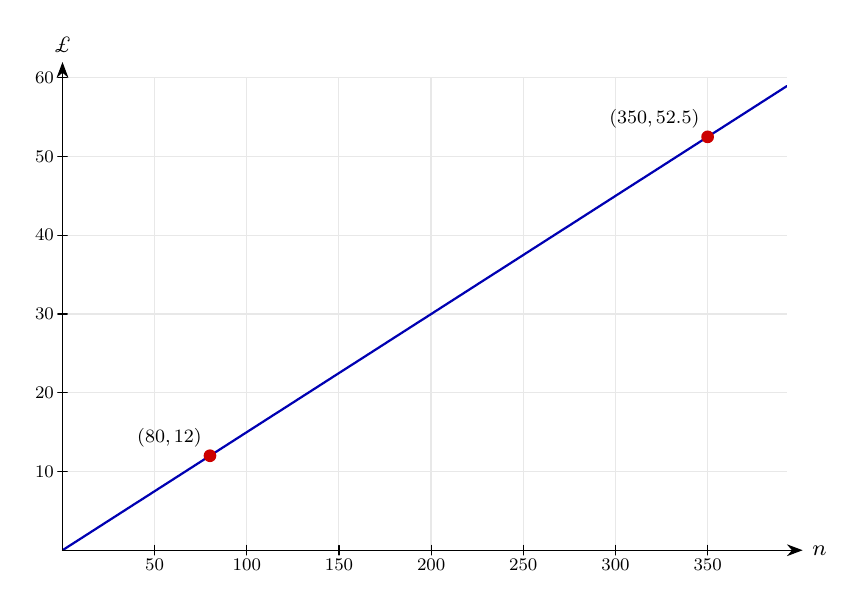
\begin{tikzpicture}[>={Stealth[length=2mm]},font=\footnotesize,line cap=round,line join=round]
\begin{scope}
\clip (0,0) rectangle (9.2,6);
\draw[gray!18] (0,0) grid[xstep=1.17,ystep=1] (9.2,6);
\draw[blue!70!black,thick] (0,0) -- (0.046,0.029) -- (0.092,0.059) -- (0.138,0.088) -- (0.184,0.118) -- (0.23,0.147) -- (0.276,0.177) -- (0.322,0.206) -- (0.368,0.236) -- (0.414,0.265) -- (0.46,0.295) -- (0.506,0.324) -- (0.552,0.354) -- (0.598,0.383) -- (0.644,0.413) -- (0.69,0.442) -- (0.736,0.472) -- (0.782,0.501) -- (0.828,0.531) -- (0.874,0.56) -- (0.92,0.59) -- (0.966,0.619) -- (1.012,0.648) -- (1.058,0.678) -- (1.104,0.707) -- (1.15,0.737) -- (1.196,0.766) -- (1.242,0.796) -- (1.288,0.825) -- (1.334,0.855) -- (1.38,0.884) -- (1.426,0.914) -- (1.472,0.943) -- (1.518,0.973) -- (1.564,1.002) -- (1.61,1.032) -- (1.656,1.061) -- (1.702,1.091) -- (1.748,1.12) -- (1.794,1.15) -- (1.84,1.179) -- (1.886,1.208) -- (1.932,1.238) -- (1.978,1.267) -- (2.024,1.297) -- (2.07,1.326) -- (2.116,1.356) -- (2.162,1.385) -- (2.208,1.415) -- (2.254,1.444) -- (2.3,1.474) -- (2.346,1.503) -- (2.392,1.533) -- (2.438,1.562) -- (2.484,1.592) -- (2.53,1.621) -- (2.576,1.651) -- (2.622,1.68) -- (2.668,1.71) -- (2.714,1.739) -- (2.76,1.768) -- (2.806,1.798) -- (2.852,1.827) -- (2.898,1.857) -- (2.944,1.886) -- (2.99,1.916) -- (3.036,1.945) -- (3.082,1.975) -- (3.128,2.004) -- (3.174,2.034) -- (3.22,2.063) -- (3.266,2.093) -- (3.312,2.122) -- (3.358,2.152) -- (3.404,2.181) -- (3.45,2.211) -- (3.496,2.24) -- (3.542,2.27) -- (3.588,2.299) -- (3.634,2.329) -- (3.68,2.358) -- (3.726,2.387) -- (3.772,2.417) -- (3.818,2.446) -- (3.864,2.476) -- (3.91,2.505) -- (3.956,2.535) -- (4.002,2.564) -- (4.048,2.594) -- (4.094,2.623) -- (4.14,2.653) -- (4.186,2.682) -- (4.232,2.712) -- (4.278,2.741) -- (4.324,2.771) -- (4.37,2.8) -- (4.416,2.83) -- (4.462,2.859) -- (4.508,2.889) -- (4.554,2.918) -- (4.6,2.947) -- (4.646,2.977) -- (4.692,3.006) -- (4.738,3.036) -- (4.784,3.065) -- (4.83,3.095) -- (4.876,3.124) -- (4.922,3.154) -- (4.968,3.183) -- (5.014,3.213) -- (5.06,3.242) -- (5.106,3.272) -- (5.152,3.301) -- (5.198,3.331) -- (5.244,3.36) -- (5.29,3.39) -- (5.336,3.419) -- (5.382,3.449) -- (5.428,3.478) -- (5.474,3.508) -- (5.52,3.537) -- (5.566,3.566) -- (5.612,3.596) -- (5.658,3.625) -- (5.704,3.655) -- (5.75,3.684) -- (5.796,3.714) -- (5.842,3.743) -- (5.888,3.773) -- (5.934,3.802) -- (5.98,3.832) -- (6.026,3.861) -- (6.072,3.891) -- (6.118,3.92) -- (6.164,3.95) -- (6.21,3.979) -- (6.256,4.009) -- (6.302,4.038) -- (6.348,4.068) -- (6.394,4.097) -- (6.44,4.126) -- (6.486,4.156) -- (6.532,4.185) -- (6.578,4.215) -- (6.624,4.244) -- (6.67,4.274) -- (6.716,4.303) -- (6.762,4.333) -- (6.808,4.362) -- (6.854,4.392) -- (6.9,4.421) -- (6.946,4.451) -- (6.992,4.48) -- (7.038,4.51) -- (7.084,4.539) -- (7.13,4.569) -- (7.176,4.598) -- (7.222,4.628) -- (7.268,4.657) -- (7.314,4.687) -- (7.36,4.716) -- (7.406,4.745) -- (7.452,4.775) -- (7.498,4.804) -- (7.544,4.834) -- (7.59,4.863) -- (7.636,4.893) -- (7.682,4.922) -- (7.728,4.952) -- (7.774,4.981) -- (7.82,5.011) -- (7.866,5.04) -- (7.912,5.07) -- (7.958,5.099) -- (8.004,5.129) -- (8.05,5.158) -- (8.096,5.188) -- (8.142,5.217) -- (8.188,5.247) -- (8.234,5.276) -- (8.28,5.306) -- (8.326,5.335) -- (8.372,5.364) -- (8.418,5.394) -- (8.464,5.423) -- (8.51,5.453) -- (8.556,5.482) -- (8.602,5.512) -- (8.648,5.541) -- (8.694,5.571) -- (8.74,5.6) -- (8.786,5.63) -- (8.832,5.659) -- (8.878,5.689) -- (8.924,5.718) -- (8.97,5.748) -- (9.016,5.777) -- (9.062,5.807) -- (9.108,5.836) -- (9.154,5.866) -- (9.2,5.895);
\end{scope}
\draw[->] (0,0) -- (9.4,0) node[right]{$n$};
\draw[->] (0,0) -- (0,6.2) node[above]{$\pounds$};
\draw (1.17,-0.06) -- (1.17,0.06) node[below=2pt,scale=0.8]{$50$};
\draw (2.341,-0.06) -- (2.341,0.06) node[below=2pt,scale=0.8]{$100$};
\draw (3.511,-0.06) -- (3.511,0.06) node[below=2pt,scale=0.8]{$150$};
\draw (4.682,-0.06) -- (4.682,0.06) node[below=2pt,scale=0.8]{$200$};
\draw (5.852,-0.06) -- (5.852,0.06) node[below=2pt,scale=0.8]{$250$};
\draw (7.023,-0.06) -- (7.023,0.06) node[below=2pt,scale=0.8]{$300$};
\draw (8.193,-0.06) -- (8.193,0.06) node[below=2pt,scale=0.8]{$350$};
\draw (-0.06,1) -- (0.06,1) node[left=2pt,scale=0.8]{$10$};
\draw (-0.06,2) -- (0.06,2) node[left=2pt,scale=0.8]{$20$};
\draw (-0.06,3) -- (0.06,3) node[left=2pt,scale=0.8]{$30$};
\draw (-0.06,4) -- (0.06,4) node[left=2pt,scale=0.8]{$40$};
\draw (-0.06,5) -- (0.06,5) node[left=2pt,scale=0.8]{$50$};
\draw (-0.06,6) -- (0.06,6) node[left=2pt,scale=0.8]{$60$};
\fill[red!80!black] (1.873,1.2) circle (2.3pt);
\node[above left,scale=0.85] at (1.873,1.2) {$(80,12)$};
\fill[red!80!black] (8.193,5.25) circle (2.3pt);
\node[above left,scale=0.85] at (8.193,5.25) {$(350,52.5)$};
\end{tikzpicture}
}
\end{center}
\small The relationship plotted, with the data points marked.\normalsize

\medskip\hrule

\section*{Proportion 08\quad\small\texttt{(cg4-008)}}
\addcontentsline{toc}{section}{Proportion 08 (cg4-008)}
\textit{Difficulty: Foundation \quad\textbar\quad Marks: 5}

\question{The extension \( e \) cm of a spring is directly proportional to the force \( F \) N applied to it. The spring extends 6 cm when a force of 15 N is applied. \\[3pt] a) Find the equation connecting \( e \) and \( F \). \\[3pt] b) Find the extension when a force of 40 N is applied. \\[3pt] c) Find the force needed to extend the spring by 9 cm.}

\textbf{Worked solution.}

\textit{Step 1: Write \( e = kF \) and substitute the known values.}
\[\begin{gathered}
6 = k \times 15 \implies k = \frac{6}{15} = \frac{2}{5}
\end{gathered}\]
Find the constant of proportionality.

\textit{Step 2: State the equation (part a).}
\[\begin{gathered}
e = \frac{2}{5}F
\end{gathered}\]
This is the complete relationship between \( e \) and \( F \).

\textit{Step 3: Part b: substitute \( F = 40 \).}
\[\begin{gathered}
e = \frac{2}{5} \times 40 = 16 \text{ cm}
\end{gathered}\]
The spring extends 16 cm.

\textit{Step 4: Part c: substitute \( e = 9 \) and solve for \( F \).}
\[\begin{gathered}
9 = \frac{2}{5}F \implies F = \frac{9 \times 5}{2} = 22.5 \text{ N}
\end{gathered}\]
Multiply both sides by \( \frac{5}{2} \).

\begin{answerbox}
\textbf{Final answer:}\quad a) \(\displaystyle e = \frac{2}{5}F\); b) \(\displaystyle 16\) cm; c) \(\displaystyle 22.5\) N
\end{answerbox}
\textbf{Graph.}

\begin{center}
\resizebox{\ifdim\width>\linewidth \linewidth\else \width\fi}{!}{%
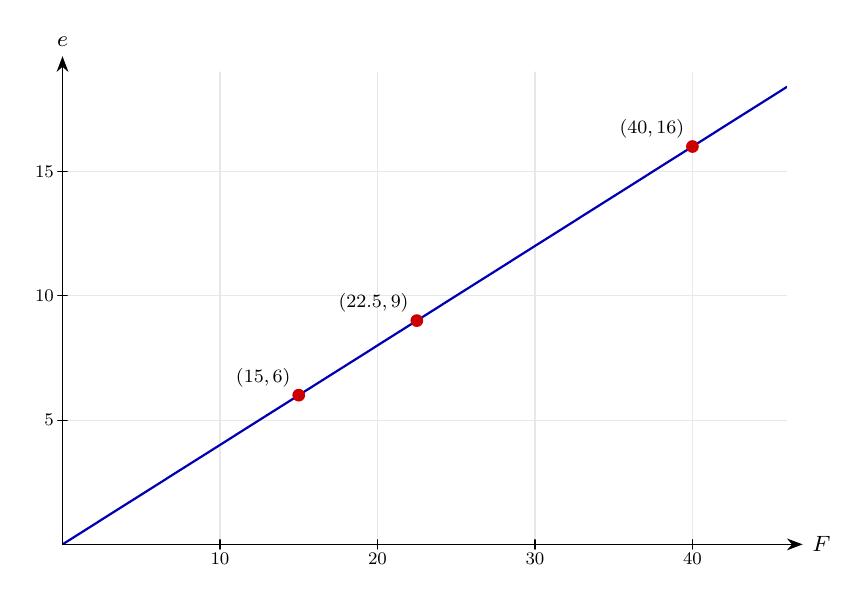
\begin{tikzpicture}[>={Stealth[length=2mm]},font=\footnotesize,line cap=round,line join=round]
\begin{scope}
\clip (0,0) rectangle (9.2,6);
\draw[gray!18] (0,0) grid[xstep=2,ystep=1.579] (9.2,6);
\draw[blue!70!black,thick] (0,0) -- (0.046,0.029) -- (0.092,0.058) -- (0.138,0.087) -- (0.184,0.116) -- (0.23,0.145) -- (0.276,0.174) -- (0.322,0.203) -- (0.368,0.232) -- (0.414,0.261) -- (0.46,0.291) -- (0.506,0.32) -- (0.552,0.349) -- (0.598,0.378) -- (0.644,0.407) -- (0.69,0.436) -- (0.736,0.465) -- (0.782,0.494) -- (0.828,0.523) -- (0.874,0.552) -- (0.92,0.581) -- (0.966,0.61) -- (1.012,0.639) -- (1.058,0.668) -- (1.104,0.697) -- (1.15,0.726) -- (1.196,0.755) -- (1.242,0.784) -- (1.288,0.813) -- (1.334,0.843) -- (1.38,0.872) -- (1.426,0.901) -- (1.472,0.93) -- (1.518,0.959) -- (1.564,0.988) -- (1.61,1.017) -- (1.656,1.046) -- (1.702,1.075) -- (1.748,1.104) -- (1.794,1.133) -- (1.84,1.162) -- (1.886,1.191) -- (1.932,1.22) -- (1.978,1.249) -- (2.024,1.278) -- (2.07,1.307) -- (2.116,1.336) -- (2.162,1.365) -- (2.208,1.395) -- (2.254,1.424) -- (2.3,1.453) -- (2.346,1.482) -- (2.392,1.511) -- (2.438,1.54) -- (2.484,1.569) -- (2.53,1.598) -- (2.576,1.627) -- (2.622,1.656) -- (2.668,1.685) -- (2.714,1.714) -- (2.76,1.743) -- (2.806,1.772) -- (2.852,1.801) -- (2.898,1.83) -- (2.944,1.859) -- (2.99,1.888) -- (3.036,1.917) -- (3.082,1.947) -- (3.128,1.976) -- (3.174,2.005) -- (3.22,2.034) -- (3.266,2.063) -- (3.312,2.092) -- (3.358,2.121) -- (3.404,2.15) -- (3.45,2.179) -- (3.496,2.208) -- (3.542,2.237) -- (3.588,2.266) -- (3.634,2.295) -- (3.68,2.324) -- (3.726,2.353) -- (3.772,2.382) -- (3.818,2.411) -- (3.864,2.44) -- (3.91,2.469) -- (3.956,2.499) -- (4.002,2.528) -- (4.048,2.557) -- (4.094,2.586) -- (4.14,2.615) -- (4.186,2.644) -- (4.232,2.673) -- (4.278,2.702) -- (4.324,2.731) -- (4.37,2.76) -- (4.416,2.789) -- (4.462,2.818) -- (4.508,2.847) -- (4.554,2.876) -- (4.6,2.905) -- (4.646,2.934) -- (4.692,2.963) -- (4.738,2.992) -- (4.784,3.021) -- (4.83,3.051) -- (4.876,3.08) -- (4.922,3.109) -- (4.968,3.138) -- (5.014,3.167) -- (5.06,3.196) -- (5.106,3.225) -- (5.152,3.254) -- (5.198,3.283) -- (5.244,3.312) -- (5.29,3.341) -- (5.336,3.37) -- (5.382,3.399) -- (5.428,3.428) -- (5.474,3.457) -- (5.52,3.486) -- (5.566,3.515) -- (5.612,3.544) -- (5.658,3.573) -- (5.704,3.603) -- (5.75,3.632) -- (5.796,3.661) -- (5.842,3.69) -- (5.888,3.719) -- (5.934,3.748) -- (5.98,3.777) -- (6.026,3.806) -- (6.072,3.835) -- (6.118,3.864) -- (6.164,3.893) -- (6.21,3.922) -- (6.256,3.951) -- (6.302,3.98) -- (6.348,4.009) -- (6.394,4.038) -- (6.44,4.067) -- (6.486,4.096) -- (6.532,4.125) -- (6.578,4.155) -- (6.624,4.184) -- (6.67,4.213) -- (6.716,4.242) -- (6.762,4.271) -- (6.808,4.3) -- (6.854,4.329) -- (6.9,4.358) -- (6.946,4.387) -- (6.992,4.416) -- (7.038,4.445) -- (7.084,4.474) -- (7.13,4.503) -- (7.176,4.532) -- (7.222,4.561) -- (7.268,4.59) -- (7.314,4.619) -- (7.36,4.648) -- (7.406,4.677) -- (7.452,4.707) -- (7.498,4.736) -- (7.544,4.765) -- (7.59,4.794) -- (7.636,4.823) -- (7.682,4.852) -- (7.728,4.881) -- (7.774,4.91) -- (7.82,4.939) -- (7.866,4.968) -- (7.912,4.997) -- (7.958,5.026) -- (8.004,5.055) -- (8.05,5.084) -- (8.096,5.113) -- (8.142,5.142) -- (8.188,5.171) -- (8.234,5.2) -- (8.28,5.229) -- (8.326,5.259) -- (8.372,5.288) -- (8.418,5.317) -- (8.464,5.346) -- (8.51,5.375) -- (8.556,5.404) -- (8.602,5.433) -- (8.648,5.462) -- (8.694,5.491) -- (8.74,5.52) -- (8.786,5.549) -- (8.832,5.578) -- (8.878,5.607) -- (8.924,5.636) -- (8.97,5.665) -- (9.016,5.694) -- (9.062,5.723) -- (9.108,5.752) -- (9.154,5.781) -- (9.2,5.811);
\end{scope}
\draw[->] (0,0) -- (9.4,0) node[right]{$F$};
\draw[->] (0,0) -- (0,6.2) node[above]{$e$};
\draw (2,-0.06) -- (2,0.06) node[below=2pt,scale=0.8]{$10$};
\draw (4,-0.06) -- (4,0.06) node[below=2pt,scale=0.8]{$20$};
\draw (6,-0.06) -- (6,0.06) node[below=2pt,scale=0.8]{$30$};
\draw (8,-0.06) -- (8,0.06) node[below=2pt,scale=0.8]{$40$};
\draw (-0.06,1.579) -- (0.06,1.579) node[left=2pt,scale=0.8]{$5$};
\draw (-0.06,3.158) -- (0.06,3.158) node[left=2pt,scale=0.8]{$10$};
\draw (-0.06,4.737) -- (0.06,4.737) node[left=2pt,scale=0.8]{$15$};
\fill[red!80!black] (3,1.895) circle (2.3pt);
\node[above left,scale=0.85] at (3,1.895) {$(15,6)$};
\fill[red!80!black] (8,5.053) circle (2.3pt);
\node[above left,scale=0.85] at (8,5.053) {$(40,16)$};
\fill[red!80!black] (4.5,2.842) circle (2.3pt);
\node[above left,scale=0.85] at (4.5,2.842) {$(22.5,9)$};
\end{tikzpicture}
}
\end{center}
\small The relationship plotted, with the data points marked.\normalsize

\medskip\hrule

\section*{Proportion 09\quad\small\texttt{(cg4-009)}}
\addcontentsline{toc}{section}{Proportion 09 (cg4-009)}
\textit{Difficulty: Foundation \quad\textbar\quad Marks: 3}

\question{Given that \( y \) is inversely proportional to \( x \), and that \( y = 8 \) when \( x = 5 \), find \( y \) when \( x = 20 \).}

\textbf{Worked solution.}

\textit{Step 1: Write the inverse proportion equation.}
\[\begin{gathered}
y = \frac{k}{x}
\end{gathered}\]
\( y \propto \frac{1}{x} \) is equivalent to \( y = \frac{k}{x} \).

\textit{Step 2: Find \( k \) using the known pair.}
\[\begin{gathered}
8 = \frac{k}{5} \implies k = 40
\end{gathered}\]
Multiply both sides by 5.

\textit{Step 3: Substitute \( x = 20 \).}
\[\begin{gathered}
y = \frac{40}{20} = 2
\end{gathered}\]
When \( x \) increases by a factor of 4, \( y \) decreases by a factor of 4.

\begin{answerbox}
\textbf{Final answer:}\quad \(\displaystyle  y = 2 \)
\end{answerbox}
\textbf{Graph.}

\begin{center}
\resizebox{\ifdim\width>\linewidth \linewidth\else \width\fi}{!}{%
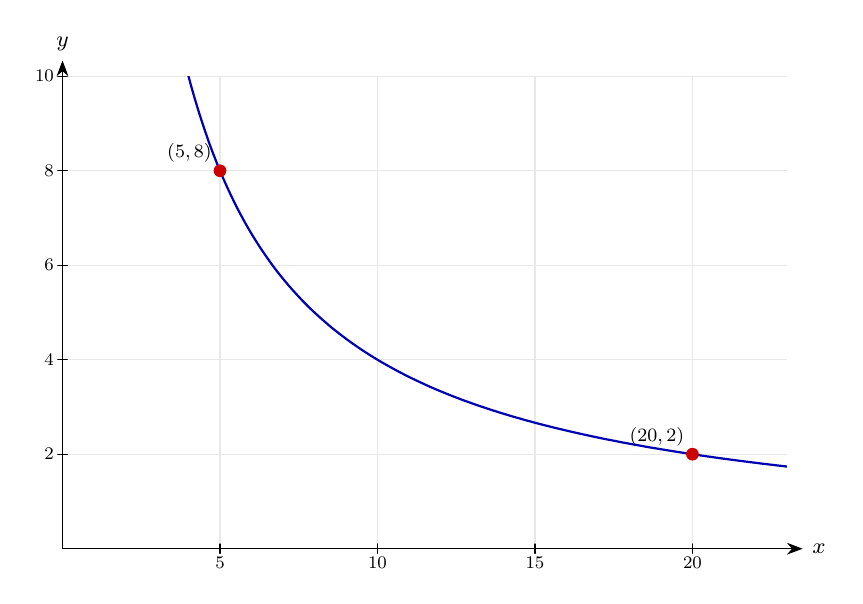
\begin{tikzpicture}[>={Stealth[length=2mm]},font=\footnotesize,line cap=round,line join=round]
\begin{scope}
\clip (0,0) rectangle (9.2,6);
\draw[gray!18] (0,0) grid[xstep=2,ystep=1.2] (9.2,6);
\draw[blue!70!black,thick] (0.023,12) -- (0.069,12) -- (0.115,12) -- (0.161,12) -- (0.207,12) -- (0.252,12) -- (0.298,12) -- (0.344,12) -- (0.39,12) -- (0.436,12) -- (0.482,12) -- (0.528,12) -- (0.574,12) -- (0.62,12) -- (0.665,12) -- (0.711,12) -- (0.757,12) -- (0.803,11.954) -- (0.849,11.308) -- (0.895,10.728) -- (0.941,10.205) -- (0.987,9.731) -- (1.032,9.298) -- (1.078,8.902) -- (1.124,8.539) -- (1.17,8.204) -- (1.216,7.895) -- (1.262,7.608) -- (1.308,7.341) -- (1.354,7.092) -- (1.4,6.859) -- (1.445,6.642) -- (1.491,6.437) -- (1.537,6.245) -- (1.583,6.064) -- (1.629,5.893) -- (1.675,5.732) -- (1.721,5.579) -- (1.767,5.434) -- (1.813,5.297) -- (1.858,5.166) -- (1.904,5.041) -- (1.95,4.923) -- (1.996,4.809) -- (2.042,4.701) -- (2.088,4.598) -- (2.134,4.499) -- (2.18,4.404) -- (2.225,4.314) -- (2.271,4.227) -- (2.317,4.143) -- (2.363,4.062) -- (2.409,3.985) -- (2.455,3.911) -- (2.501,3.839) -- (2.547,3.77) -- (2.593,3.703) -- (2.638,3.639) -- (2.684,3.576) -- (2.73,3.516) -- (2.776,3.458) -- (2.822,3.402) -- (2.868,3.347) -- (2.914,3.295) -- (2.96,3.244) -- (3.006,3.194) -- (3.051,3.146) -- (3.097,3.099) -- (3.143,3.054) -- (3.189,3.01) -- (3.235,2.968) -- (3.281,2.926) -- (3.327,2.886) -- (3.373,2.846) -- (3.418,2.808) -- (3.464,2.771) -- (3.51,2.735) -- (3.556,2.7) -- (3.602,2.665) -- (3.648,2.632) -- (3.694,2.599) -- (3.74,2.567) -- (3.786,2.536) -- (3.831,2.506) -- (3.877,2.476) -- (3.923,2.447) -- (3.969,2.419) -- (4.015,2.391) -- (4.061,2.364) -- (4.107,2.338) -- (4.153,2.312) -- (4.199,2.287) -- (4.244,2.262) -- (4.29,2.238) -- (4.336,2.214) -- (4.382,2.191) -- (4.428,2.168) -- (4.474,2.146) -- (4.52,2.124) -- (4.566,2.103) -- (4.611,2.082) -- (4.657,2.061) -- (4.703,2.041) -- (4.749,2.021) -- (4.795,2.002) -- (4.841,1.983) -- (4.887,1.964) -- (4.933,1.946) -- (4.979,1.928) -- (5.024,1.911) -- (5.07,1.893) -- (5.116,1.876) -- (5.162,1.86) -- (5.208,1.843) -- (5.254,1.827) -- (5.3,1.811) -- (5.346,1.796) -- (5.392,1.781) -- (5.437,1.766) -- (5.483,1.751) -- (5.529,1.736) -- (5.575,1.722) -- (5.621,1.708) -- (5.667,1.694) -- (5.713,1.68) -- (5.759,1.667) -- (5.805,1.654) -- (5.85,1.641) -- (5.896,1.628) -- (5.942,1.616) -- (5.988,1.603) -- (6.034,1.591) -- (6.08,1.579) -- (6.126,1.567) -- (6.172,1.556) -- (6.217,1.544) -- (6.263,1.533) -- (6.309,1.522) -- (6.355,1.511) -- (6.401,1.5) -- (6.447,1.489) -- (6.493,1.479) -- (6.539,1.468) -- (6.585,1.458) -- (6.63,1.448) -- (6.676,1.438) -- (6.722,1.428) -- (6.768,1.418) -- (6.814,1.409) -- (6.86,1.399) -- (6.906,1.39) -- (6.952,1.381) -- (6.998,1.372) -- (7.043,1.363) -- (7.089,1.354) -- (7.135,1.345) -- (7.181,1.337) -- (7.227,1.328) -- (7.273,1.32) -- (7.319,1.312) -- (7.365,1.304) -- (7.41,1.295) -- (7.456,1.287) -- (7.502,1.28) -- (7.548,1.272) -- (7.594,1.264) -- (7.64,1.257) -- (7.686,1.249) -- (7.732,1.242) -- (7.778,1.234) -- (7.823,1.227) -- (7.869,1.22) -- (7.915,1.213) -- (7.961,1.206) -- (8.007,1.199) -- (8.053,1.192) -- (8.099,1.185) -- (8.145,1.179) -- (8.191,1.172) -- (8.236,1.166) -- (8.282,1.159) -- (8.328,1.153) -- (8.374,1.146) -- (8.42,1.14) -- (8.466,1.134) -- (8.512,1.128) -- (8.558,1.122) -- (8.603,1.116) -- (8.649,1.11) -- (8.695,1.104) -- (8.741,1.098) -- (8.787,1.093) -- (8.833,1.087) -- (8.879,1.081) -- (8.925,1.076) -- (8.971,1.07) -- (9.016,1.065) -- (9.062,1.059) -- (9.108,1.054) -- (9.154,1.049) -- (9.2,1.043);
\end{scope}
\draw[->] (0,0) -- (9.4,0) node[right]{$x$};
\draw[->] (0,0) -- (0,6.2) node[above]{$y$};
\draw (2,-0.06) -- (2,0.06) node[below=2pt,scale=0.8]{$5$};
\draw (4,-0.06) -- (4,0.06) node[below=2pt,scale=0.8]{$10$};
\draw (6,-0.06) -- (6,0.06) node[below=2pt,scale=0.8]{$15$};
\draw (8,-0.06) -- (8,0.06) node[below=2pt,scale=0.8]{$20$};
\draw (-0.06,1.2) -- (0.06,1.2) node[left=2pt,scale=0.8]{$2$};
\draw (-0.06,2.4) -- (0.06,2.4) node[left=2pt,scale=0.8]{$4$};
\draw (-0.06,3.6) -- (0.06,3.6) node[left=2pt,scale=0.8]{$6$};
\draw (-0.06,4.8) -- (0.06,4.8) node[left=2pt,scale=0.8]{$8$};
\draw (-0.06,6) -- (0.06,6) node[left=2pt,scale=0.8]{$10$};
\fill[red!80!black] (2,4.8) circle (2.3pt);
\node[above left,scale=0.85] at (2,4.8) {$(5,8)$};
\fill[red!80!black] (8,1.2) circle (2.3pt);
\node[above left,scale=0.85] at (8,1.2) {$(20,2)$};
\end{tikzpicture}
}
\end{center}
\small The relationship plotted, with the data points marked.\normalsize

\medskip\hrule

\section*{Proportion 10\quad\small\texttt{(cg4-010)}}
\addcontentsline{toc}{section}{Proportion 10 (cg4-010)}
\textit{Difficulty: Foundation \quad\textbar\quad Marks: 3}

\question{Given that \( x \) and \( y \) are inversely proportional, \( y = 4 \) when \( x = 15 \), and \( y = a \) when \( x = 3 \), find \( a \).}

\textbf{Worked solution.}

\textit{Step 1: Find \( k \).}
\[\begin{gathered}
k = xy = 4 \times 15 = 60
\end{gathered}\]
For inverse proportion, \( xy = k \) is constant.

\textit{Step 2: Substitute \( x = 3 \).}
\[\begin{gathered}
a = \frac{60}{3} = 20
\end{gathered}\]
Divide the constant by the new \( x \)-value.

\begin{answerbox}
\textbf{Final answer:}\quad \(\displaystyle  a = 20 \)
\end{answerbox}
\textbf{Graph.}

\begin{center}
\resizebox{\ifdim\width>\linewidth \linewidth\else \width\fi}{!}{%
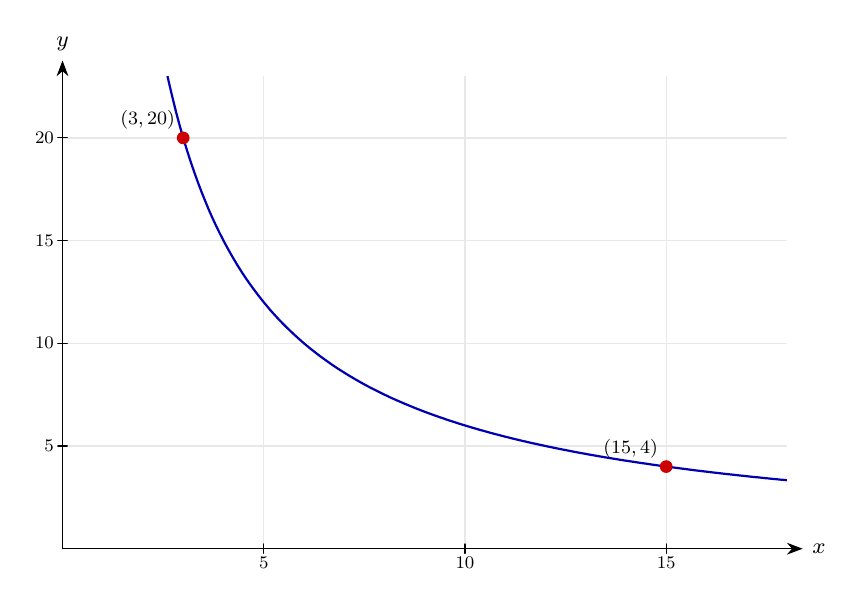
\begin{tikzpicture}[>={Stealth[length=2mm]},font=\footnotesize,line cap=round,line join=round]
\begin{scope}
\clip (0,0) rectangle (9.2,6);
\draw[gray!18] (0,0) grid[xstep=2.556,ystep=1.304] (9.2,6);
\draw[blue!70!black,thick] (0.023,12) -- (0.069,12) -- (0.115,12) -- (0.161,12) -- (0.207,12) -- (0.252,12) -- (0.298,12) -- (0.344,12) -- (0.39,12) -- (0.436,12) -- (0.482,12) -- (0.528,12) -- (0.574,12) -- (0.62,12) -- (0.665,12) -- (0.711,11.247) -- (0.757,10.566) -- (0.803,9.962) -- (0.849,9.424) -- (0.895,8.94) -- (0.941,8.504) -- (0.987,8.109) -- (1.032,7.748) -- (1.078,7.419) -- (1.124,7.116) -- (1.17,6.837) -- (1.216,6.579) -- (1.262,6.34) -- (1.308,6.117) -- (1.354,5.91) -- (1.4,5.716) -- (1.445,5.535) -- (1.491,5.364) -- (1.537,5.204) -- (1.583,5.053) -- (1.629,4.911) -- (1.675,4.777) -- (1.721,4.649) -- (1.767,4.528) -- (1.813,4.414) -- (1.858,4.305) -- (1.904,4.201) -- (1.95,4.102) -- (1.996,4.008) -- (2.042,3.918) -- (2.088,3.832) -- (2.134,3.749) -- (2.18,3.67) -- (2.225,3.595) -- (2.271,3.522) -- (2.317,3.452) -- (2.363,3.385) -- (2.409,3.321) -- (2.455,3.259) -- (2.501,3.199) -- (2.547,3.141) -- (2.593,3.086) -- (2.638,3.032) -- (2.684,2.98) -- (2.73,2.93) -- (2.776,2.882) -- (2.822,2.835) -- (2.868,2.79) -- (2.914,2.746) -- (2.96,2.703) -- (3.006,2.662) -- (3.051,2.622) -- (3.097,2.583) -- (3.143,2.545) -- (3.189,2.509) -- (3.235,2.473) -- (3.281,2.438) -- (3.327,2.405) -- (3.373,2.372) -- (3.418,2.34) -- (3.464,2.309) -- (3.51,2.279) -- (3.556,2.25) -- (3.602,2.221) -- (3.648,2.193) -- (3.694,2.166) -- (3.74,2.139) -- (3.786,2.113) -- (3.831,2.088) -- (3.877,2.063) -- (3.923,2.039) -- (3.969,2.016) -- (4.015,1.993) -- (4.061,1.97) -- (4.107,1.948) -- (4.153,1.926) -- (4.199,1.905) -- (4.244,1.885) -- (4.29,1.865) -- (4.336,1.845) -- (4.382,1.826) -- (4.428,1.807) -- (4.474,1.788) -- (4.52,1.77) -- (4.566,1.752) -- (4.611,1.735) -- (4.657,1.718) -- (4.703,1.701) -- (4.749,1.685) -- (4.795,1.668) -- (4.841,1.653) -- (4.887,1.637) -- (4.933,1.622) -- (4.979,1.607) -- (5.024,1.592) -- (5.07,1.578) -- (5.116,1.564) -- (5.162,1.55) -- (5.208,1.536) -- (5.254,1.523) -- (5.3,1.509) -- (5.346,1.497) -- (5.392,1.484) -- (5.437,1.471) -- (5.483,1.459) -- (5.529,1.447) -- (5.575,1.435) -- (5.621,1.423) -- (5.667,1.412) -- (5.713,1.4) -- (5.759,1.389) -- (5.805,1.378) -- (5.85,1.367) -- (5.896,1.357) -- (5.942,1.346) -- (5.988,1.336) -- (6.034,1.326) -- (6.08,1.316) -- (6.126,1.306) -- (6.172,1.296) -- (6.217,1.287) -- (6.263,1.277) -- (6.309,1.268) -- (6.355,1.259) -- (6.401,1.25) -- (6.447,1.241) -- (6.493,1.232) -- (6.539,1.223) -- (6.585,1.215) -- (6.63,1.207) -- (6.676,1.198) -- (6.722,1.19) -- (6.768,1.182) -- (6.814,1.174) -- (6.86,1.166) -- (6.906,1.158) -- (6.952,1.151) -- (6.998,1.143) -- (7.043,1.136) -- (7.089,1.128) -- (7.135,1.121) -- (7.181,1.114) -- (7.227,1.107) -- (7.273,1.1) -- (7.319,1.093) -- (7.365,1.086) -- (7.41,1.08) -- (7.456,1.073) -- (7.502,1.066) -- (7.548,1.06) -- (7.594,1.053) -- (7.64,1.047) -- (7.686,1.041) -- (7.732,1.035) -- (7.778,1.029) -- (7.823,1.023) -- (7.869,1.017) -- (7.915,1.011) -- (7.961,1.005) -- (8.007,0.999) -- (8.053,0.993) -- (8.099,0.988) -- (8.145,0.982) -- (8.191,0.977) -- (8.236,0.971) -- (8.282,0.966) -- (8.328,0.961) -- (8.374,0.955) -- (8.42,0.95) -- (8.466,0.945) -- (8.512,0.94) -- (8.558,0.935) -- (8.603,0.93) -- (8.649,0.925) -- (8.695,0.92) -- (8.741,0.915) -- (8.787,0.91) -- (8.833,0.906) -- (8.879,0.901) -- (8.925,0.896) -- (8.971,0.892) -- (9.016,0.887) -- (9.062,0.883) -- (9.108,0.878) -- (9.154,0.874) -- (9.2,0.87);
\end{scope}
\draw[->] (0,0) -- (9.4,0) node[right]{$x$};
\draw[->] (0,0) -- (0,6.2) node[above]{$y$};
\draw (2.556,-0.06) -- (2.556,0.06) node[below=2pt,scale=0.8]{$5$};
\draw (5.111,-0.06) -- (5.111,0.06) node[below=2pt,scale=0.8]{$10$};
\draw (7.667,-0.06) -- (7.667,0.06) node[below=2pt,scale=0.8]{$15$};
\draw (-0.06,1.304) -- (0.06,1.304) node[left=2pt,scale=0.8]{$5$};
\draw (-0.06,2.609) -- (0.06,2.609) node[left=2pt,scale=0.8]{$10$};
\draw (-0.06,3.913) -- (0.06,3.913) node[left=2pt,scale=0.8]{$15$};
\draw (-0.06,5.217) -- (0.06,5.217) node[left=2pt,scale=0.8]{$20$};
\fill[red!80!black] (7.667,1.043) circle (2.3pt);
\node[above left,scale=0.85] at (7.667,1.043) {$(15,4)$};
\fill[red!80!black] (1.533,5.217) circle (2.3pt);
\node[above left,scale=0.85] at (1.533,5.217) {$(3,20)$};
\end{tikzpicture}
}
\end{center}
\small The relationship plotted, with the data points marked.\normalsize

\medskip\hrule

\section*{Proportion 11\quad\small\texttt{(cg4-011)}}
\addcontentsline{toc}{section}{Proportion 11 (cg4-011)}
\textit{Difficulty: Foundation \quad\textbar\quad Marks: 3}

\question{The time \( t \) hours to complete a journey is inversely proportional to the average speed \( v \) km/h. A journey takes 3 hours at 80 km/h. How long does it take at 60 km/h?}

\textbf{Worked solution.}

\textit{Step 1: Write \( t = \frac{k}{v} \) and find \( k \).}
\[\begin{gathered}
k = t \times v = 3 \times 80 = 240
\end{gathered}\]
The constant \( k \) equals distance (240 km).

\textit{Step 2: Substitute \( v = 60 \).}
\[\begin{gathered}
t = \frac{240}{60} = 4 \text{ hours}
\end{gathered}\]
A lower speed means a longer journey time.

\begin{answerbox}
\textbf{Final answer:}\quad \(\displaystyle  4 \) hours
\end{answerbox}
\textbf{Graph.}

\begin{center}
\resizebox{\ifdim\width>\linewidth \linewidth\else \width\fi}{!}{%
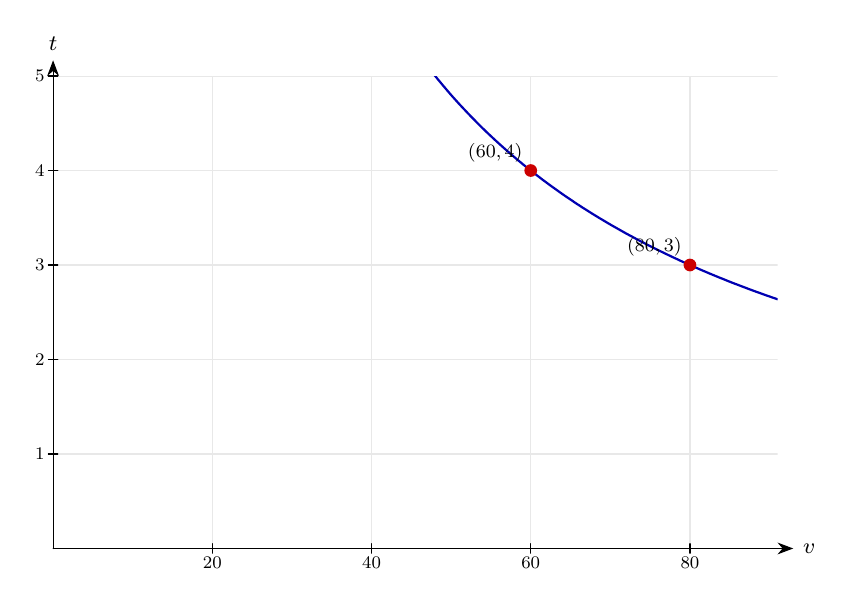
\begin{tikzpicture}[>={Stealth[length=2mm]},font=\footnotesize,line cap=round,line join=round]
\begin{scope}
\clip (0,0) rectangle (9.2,6);
\draw[gray!18] (0,0) grid[xstep=2.022,ystep=1.2] (9.2,6);
\draw[blue!70!black,thick] (0.023,12) -- (0.069,12) -- (0.115,12) -- (0.161,12) -- (0.207,12) -- (0.252,12) -- (0.298,12) -- (0.344,12) -- (0.39,12) -- (0.436,12) -- (0.482,12) -- (0.528,12) -- (0.574,12) -- (0.62,12) -- (0.665,12) -- (0.711,12) -- (0.757,12) -- (0.803,12) -- (0.849,12) -- (0.895,12) -- (0.941,12) -- (0.987,12) -- (1.032,12) -- (1.078,12) -- (1.124,12) -- (1.17,12) -- (1.216,12) -- (1.262,12) -- (1.308,12) -- (1.354,12) -- (1.4,12) -- (1.445,12) -- (1.491,12) -- (1.537,12) -- (1.583,12) -- (1.629,12) -- (1.675,12) -- (1.721,12) -- (1.767,12) -- (1.813,12) -- (1.858,12) -- (1.904,12) -- (1.95,12) -- (1.996,12) -- (2.042,12) -- (2.088,12) -- (2.134,12) -- (2.18,12) -- (2.225,12) -- (2.271,12) -- (2.317,12) -- (2.363,12) -- (2.409,12) -- (2.455,11.861) -- (2.501,11.643) -- (2.547,11.433) -- (2.593,11.231) -- (2.638,11.035) -- (2.684,10.847) -- (2.73,10.665) -- (2.776,10.488) -- (2.822,10.318) -- (2.868,10.153) -- (2.914,9.993) -- (2.96,9.838) -- (3.006,9.688) -- (3.051,9.542) -- (3.097,9.401) -- (3.143,9.263) -- (3.189,9.13) -- (3.235,9.001) -- (3.281,8.875) -- (3.327,8.752) -- (3.373,8.633) -- (3.418,8.517) -- (3.464,8.405) -- (3.51,8.295) -- (3.556,8.188) -- (3.602,8.083) -- (3.648,7.982) -- (3.694,7.883) -- (3.74,7.786) -- (3.786,7.691) -- (3.831,7.599) -- (3.877,7.509) -- (3.923,7.422) -- (3.969,7.336) -- (4.015,7.252) -- (4.061,7.17) -- (4.107,7.09) -- (4.153,7.012) -- (4.199,6.935) -- (4.244,6.86) -- (4.29,6.787) -- (4.336,6.715) -- (4.382,6.644) -- (4.428,6.576) -- (4.474,6.508) -- (4.52,6.442) -- (4.566,6.377) -- (4.611,6.314) -- (4.657,6.252) -- (4.703,6.191) -- (4.749,6.131) -- (4.795,6.072) -- (4.841,6.015) -- (4.887,5.958) -- (4.933,5.903) -- (4.979,5.848) -- (5.024,5.795) -- (5.07,5.742) -- (5.116,5.691) -- (5.162,5.64) -- (5.208,5.591) -- (5.254,5.542) -- (5.3,5.494) -- (5.346,5.447) -- (5.392,5.4) -- (5.437,5.355) -- (5.483,5.31) -- (5.529,5.266) -- (5.575,5.223) -- (5.621,5.18) -- (5.667,5.138) -- (5.713,5.097) -- (5.759,5.056) -- (5.805,5.016) -- (5.85,4.977) -- (5.896,4.938) -- (5.942,4.9) -- (5.988,4.862) -- (6.034,4.825) -- (6.08,4.789) -- (6.126,4.753) -- (6.172,4.718) -- (6.217,4.683) -- (6.263,4.649) -- (6.309,4.615) -- (6.355,4.582) -- (6.401,4.549) -- (6.447,4.516) -- (6.493,4.484) -- (6.539,4.453) -- (6.585,4.422) -- (6.63,4.391) -- (6.676,4.361) -- (6.722,4.331) -- (6.768,4.302) -- (6.814,4.273) -- (6.86,4.244) -- (6.906,4.216) -- (6.952,4.188) -- (6.998,4.161) -- (7.043,4.134) -- (7.089,4.107) -- (7.135,4.081) -- (7.181,4.055) -- (7.227,4.029) -- (7.273,4.003) -- (7.319,3.978) -- (7.365,3.954) -- (7.41,3.929) -- (7.456,3.905) -- (7.502,3.881) -- (7.548,3.857) -- (7.594,3.834) -- (7.64,3.811) -- (7.686,3.788) -- (7.732,3.766) -- (7.778,3.744) -- (7.823,3.722) -- (7.869,3.7) -- (7.915,3.679) -- (7.961,3.657) -- (8.007,3.636) -- (8.053,3.616) -- (8.099,3.595) -- (8.145,3.575) -- (8.191,3.555) -- (8.236,3.535) -- (8.282,3.516) -- (8.328,3.496) -- (8.374,3.477) -- (8.42,3.458) -- (8.466,3.439) -- (8.512,3.421) -- (8.558,3.402) -- (8.603,3.384) -- (8.649,3.366) -- (8.695,3.349) -- (8.741,3.331) -- (8.787,3.314) -- (8.833,3.296) -- (8.879,3.279) -- (8.925,3.262) -- (8.971,3.246) -- (9.016,3.229) -- (9.062,3.213) -- (9.108,3.197) -- (9.154,3.181) -- (9.2,3.165);
\end{scope}
\draw[->] (0,0) -- (9.4,0) node[right]{$v$};
\draw[->] (0,0) -- (0,6.2) node[above]{$t$};
\draw (2.022,-0.06) -- (2.022,0.06) node[below=2pt,scale=0.8]{$20$};
\draw (4.044,-0.06) -- (4.044,0.06) node[below=2pt,scale=0.8]{$40$};
\draw (6.066,-0.06) -- (6.066,0.06) node[below=2pt,scale=0.8]{$60$};
\draw (8.088,-0.06) -- (8.088,0.06) node[below=2pt,scale=0.8]{$80$};
\draw (-0.06,1.2) -- (0.06,1.2) node[left=2pt,scale=0.8]{$1$};
\draw (-0.06,2.4) -- (0.06,2.4) node[left=2pt,scale=0.8]{$2$};
\draw (-0.06,3.6) -- (0.06,3.6) node[left=2pt,scale=0.8]{$3$};
\draw (-0.06,4.8) -- (0.06,4.8) node[left=2pt,scale=0.8]{$4$};
\draw (-0.06,6) -- (0.06,6) node[left=2pt,scale=0.8]{$5$};
\fill[red!80!black] (8.088,3.6) circle (2.3pt);
\node[above left,scale=0.85] at (8.088,3.6) {$(80,3)$};
\fill[red!80!black] (6.066,4.8) circle (2.3pt);
\node[above left,scale=0.85] at (6.066,4.8) {$(60,4)$};
\end{tikzpicture}
}
\end{center}
\small The relationship plotted, with the data points marked.\normalsize

\medskip\hrule

\section*{Proportion 12\quad\small\texttt{(cg4-012)}}
\addcontentsline{toc}{section}{Proportion 12 (cg4-012)}
\textit{Difficulty: Foundation \quad\textbar\quad Marks: 3}

\question{Given that \( y \propto \dfrac{1}{x} \), that \( y = 9 \) when \( x = 4 \), and that \( y = 36 \) when \( x = a \), find \( a \).}

\textbf{Worked solution.}

\textit{Step 1: Find the constant \( k = xy \).}
\[\begin{gathered}
k = 9 \times 4 = 36
\end{gathered}\]
For inverse proportion \( xy \) is always equal to \( k \).

\textit{Step 2: Use the second pair to find \( a \).}
\[\begin{gathered}
36 \times a = 36 \implies a = 1
\end{gathered}\]
Divide both sides by 36.

\begin{answerbox}
\textbf{Final answer:}\quad \(\displaystyle  a = 1 \)
\end{answerbox}
\textbf{Graph.}

\begin{center}
\resizebox{\ifdim\width>\linewidth \linewidth\else \width\fi}{!}{%
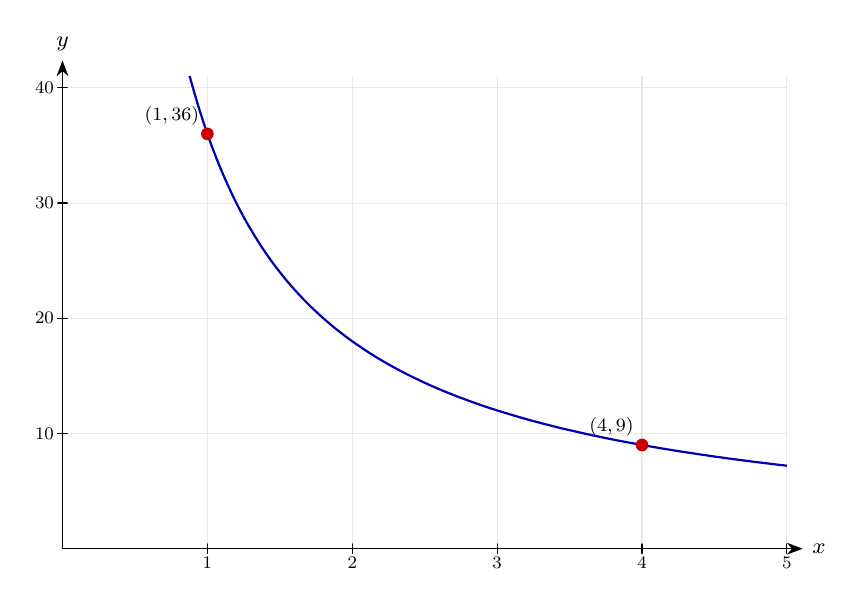
\begin{tikzpicture}[>={Stealth[length=2mm]},font=\footnotesize,line cap=round,line join=round]
\begin{scope}
\clip (0,0) rectangle (9.2,6);
\draw[gray!18] (0,0) grid[xstep=1.84,ystep=1.463] (9.2,6);
\draw[blue!70!black,thick] (0.023,12) -- (0.069,12) -- (0.115,12) -- (0.161,12) -- (0.207,12) -- (0.252,12) -- (0.298,12) -- (0.344,12) -- (0.39,12) -- (0.436,12) -- (0.482,12) -- (0.528,12) -- (0.574,12) -- (0.62,12) -- (0.665,12) -- (0.711,12) -- (0.757,12) -- (0.803,12) -- (0.849,11.419) -- (0.895,10.833) -- (0.941,10.305) -- (0.987,9.825) -- (1.032,9.389) -- (1.078,8.989) -- (1.124,8.622) -- (1.17,8.284) -- (1.216,7.972) -- (1.262,7.682) -- (1.308,7.412) -- (1.354,7.161) -- (1.4,6.926) -- (1.445,6.706) -- (1.491,6.5) -- (1.537,6.306) -- (1.583,6.123) -- (1.629,5.951) -- (1.675,5.788) -- (1.721,5.633) -- (1.767,5.487) -- (1.813,5.348) -- (1.858,5.216) -- (1.904,5.09) -- (1.95,4.971) -- (1.996,4.856) -- (2.042,4.747) -- (2.088,4.643) -- (2.134,4.543) -- (2.18,4.447) -- (2.225,4.356) -- (2.271,4.268) -- (2.317,4.183) -- (2.363,4.102) -- (2.409,4.024) -- (2.455,3.949) -- (2.501,3.876) -- (2.547,3.806) -- (2.593,3.739) -- (2.638,3.674) -- (2.684,3.611) -- (2.73,3.551) -- (2.776,3.492) -- (2.822,3.435) -- (2.868,3.38) -- (2.914,3.327) -- (2.96,3.275) -- (3.006,3.225) -- (3.051,3.177) -- (3.097,3.13) -- (3.143,3.084) -- (3.189,3.04) -- (3.235,2.997) -- (3.281,2.955) -- (3.327,2.914) -- (3.373,2.874) -- (3.418,2.836) -- (3.464,2.798) -- (3.51,2.762) -- (3.556,2.726) -- (3.602,2.691) -- (3.648,2.657) -- (3.694,2.624) -- (3.74,2.592) -- (3.786,2.561) -- (3.831,2.53) -- (3.877,2.5) -- (3.923,2.471) -- (3.969,2.442) -- (4.015,2.414) -- (4.061,2.387) -- (4.107,2.36) -- (4.153,2.334) -- (4.199,2.309) -- (4.244,2.284) -- (4.29,2.259) -- (4.336,2.236) -- (4.382,2.212) -- (4.428,2.189) -- (4.474,2.167) -- (4.52,2.145) -- (4.566,2.123) -- (4.611,2.102) -- (4.657,2.081) -- (4.703,2.061) -- (4.749,2.041) -- (4.795,2.022) -- (4.841,2.002) -- (4.887,1.984) -- (4.933,1.965) -- (4.979,1.947) -- (5.024,1.929) -- (5.07,1.912) -- (5.116,1.895) -- (5.162,1.878) -- (5.208,1.861) -- (5.254,1.845) -- (5.3,1.829) -- (5.346,1.813) -- (5.392,1.798) -- (5.437,1.783) -- (5.483,1.768) -- (5.529,1.753) -- (5.575,1.739) -- (5.621,1.725) -- (5.667,1.711) -- (5.713,1.697) -- (5.759,1.683) -- (5.805,1.67) -- (5.85,1.657) -- (5.896,1.644) -- (5.942,1.631) -- (5.988,1.619) -- (6.034,1.607) -- (6.08,1.594) -- (6.126,1.582) -- (6.172,1.571) -- (6.217,1.559) -- (6.263,1.548) -- (6.309,1.536) -- (6.355,1.525) -- (6.401,1.514) -- (6.447,1.504) -- (6.493,1.493) -- (6.539,1.483) -- (6.585,1.472) -- (6.63,1.462) -- (6.676,1.452) -- (6.722,1.442) -- (6.768,1.432) -- (6.814,1.423) -- (6.86,1.413) -- (6.906,1.404) -- (6.952,1.394) -- (6.998,1.385) -- (7.043,1.376) -- (7.089,1.367) -- (7.135,1.359) -- (7.181,1.35) -- (7.227,1.341) -- (7.273,1.333) -- (7.319,1.325) -- (7.365,1.316) -- (7.41,1.308) -- (7.456,1.3) -- (7.502,1.292) -- (7.548,1.284) -- (7.594,1.276) -- (7.64,1.269) -- (7.686,1.261) -- (7.732,1.254) -- (7.778,1.246) -- (7.823,1.239) -- (7.869,1.232) -- (7.915,1.225) -- (7.961,1.218) -- (8.007,1.211) -- (8.053,1.204) -- (8.099,1.197) -- (8.145,1.19) -- (8.191,1.184) -- (8.236,1.177) -- (8.282,1.17) -- (8.328,1.164) -- (8.374,1.158) -- (8.42,1.151) -- (8.466,1.145) -- (8.512,1.139) -- (8.558,1.133) -- (8.603,1.127) -- (8.649,1.121) -- (8.695,1.115) -- (8.741,1.109) -- (8.787,1.103) -- (8.833,1.097) -- (8.879,1.092) -- (8.925,1.086) -- (8.971,1.081) -- (9.016,1.075) -- (9.062,1.07) -- (9.108,1.064) -- (9.154,1.059) -- (9.2,1.054);
\end{scope}
\draw[->] (0,0) -- (9.4,0) node[right]{$x$};
\draw[->] (0,0) -- (0,6.2) node[above]{$y$};
\draw (1.84,-0.06) -- (1.84,0.06) node[below=2pt,scale=0.8]{$1$};
\draw (3.68,-0.06) -- (3.68,0.06) node[below=2pt,scale=0.8]{$2$};
\draw (5.52,-0.06) -- (5.52,0.06) node[below=2pt,scale=0.8]{$3$};
\draw (7.36,-0.06) -- (7.36,0.06) node[below=2pt,scale=0.8]{$4$};
\draw (9.2,-0.06) -- (9.2,0.06) node[below=2pt,scale=0.8]{$5$};
\draw (-0.06,1.463) -- (0.06,1.463) node[left=2pt,scale=0.8]{$10$};
\draw (-0.06,2.927) -- (0.06,2.927) node[left=2pt,scale=0.8]{$20$};
\draw (-0.06,4.39) -- (0.06,4.39) node[left=2pt,scale=0.8]{$30$};
\draw (-0.06,5.854) -- (0.06,5.854) node[left=2pt,scale=0.8]{$40$};
\fill[red!80!black] (7.36,1.317) circle (2.3pt);
\node[above left,scale=0.85] at (7.36,1.317) {$(4,9)$};
\fill[red!80!black] (1.84,5.268) circle (2.3pt);
\node[above left,scale=0.85] at (1.84,5.268) {$(1,36)$};
\end{tikzpicture}
}
\end{center}
\small The relationship plotted, with the data points marked.\normalsize

\medskip\hrule

\section*{Proportion 13\quad\small\texttt{(cg4-013)}}
\addcontentsline{toc}{section}{Proportion 13 (cg4-013)}
\textit{Difficulty: Foundation \quad\textbar\quad Marks: 4}

\question{The number of days \( d \) needed to build a wall is inversely proportional to the number of workers \( w \). With 6 workers the job takes 10 days. \\[3pt] a) How many days would 4 workers take? \\[3pt] b) How many workers are needed to complete the job in 5 days?}

\textbf{Worked solution.}

\textit{Step 1: Find \( k \).}
\[\begin{gathered}
k = d \times w = 10 \times 6 = 60
\end{gathered}\]
The constant represents the total worker-days needed.

\textit{Step 2: Part a: substitute \( w = 4 \).}
\[\begin{gathered}
d = \frac{60}{4} = 15 \text{ days}
\end{gathered}\]
Fewer workers means more days.

\textit{Step 3: Part b: substitute \( d = 5 \).}
\[\begin{gathered}
w = \frac{60}{5} = 12 \text{ workers}
\end{gathered}\]
More workers means fewer days.

\begin{answerbox}
\textbf{Final answer:}\quad a) \(\displaystyle 15\) days; b) \(\displaystyle 12\) workers
\end{answerbox}
\textbf{Graph.}

\begin{center}
\resizebox{\ifdim\width>\linewidth \linewidth\else \width\fi}{!}{%
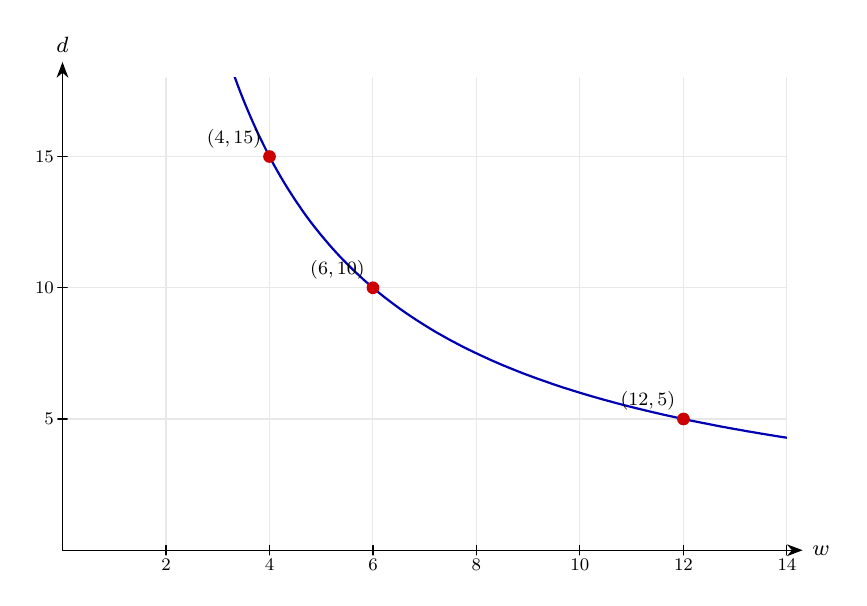
\begin{tikzpicture}[>={Stealth[length=2mm]},font=\footnotesize,line cap=round,line join=round]
\begin{scope}
\clip (0,0) rectangle (9.2,6);
\draw[gray!18] (0,0) grid[xstep=1.314,ystep=1.667] (9.2,6);
\draw[blue!70!black,thick] (0.023,12) -- (0.069,12) -- (0.115,12) -- (0.161,12) -- (0.207,12) -- (0.252,12) -- (0.298,12) -- (0.344,12) -- (0.39,12) -- (0.436,12) -- (0.482,12) -- (0.528,12) -- (0.574,12) -- (0.62,12) -- (0.665,12) -- (0.711,12) -- (0.757,12) -- (0.803,12) -- (0.849,12) -- (0.895,12) -- (0.941,12) -- (0.987,12) -- (1.032,12) -- (1.078,12) -- (1.124,11.69) -- (1.17,11.232) -- (1.216,10.808) -- (1.262,10.415) -- (1.308,10.05) -- (1.354,9.709) -- (1.4,9.391) -- (1.445,9.093) -- (1.491,8.813) -- (1.537,8.55) -- (1.583,8.302) -- (1.629,8.068) -- (1.675,7.847) -- (1.721,7.638) -- (1.767,7.44) -- (1.813,7.251) -- (1.858,7.072) -- (1.904,6.902) -- (1.95,6.739) -- (1.996,6.584) -- (2.042,6.436) -- (2.088,6.295) -- (2.134,6.16) -- (2.18,6.03) -- (2.225,5.906) -- (2.271,5.786) -- (2.317,5.672) -- (2.363,5.562) -- (2.409,5.456) -- (2.455,5.354) -- (2.501,5.255) -- (2.547,5.161) -- (2.593,5.069) -- (2.638,4.981) -- (2.684,4.896) -- (2.73,4.814) -- (2.776,4.734) -- (2.822,4.657) -- (2.868,4.583) -- (2.914,4.511) -- (2.96,4.441) -- (3.006,4.373) -- (3.051,4.307) -- (3.097,4.243) -- (3.143,4.181) -- (3.189,4.121) -- (3.235,4.063) -- (3.281,4.006) -- (3.327,3.951) -- (3.373,3.897) -- (3.418,3.845) -- (3.464,3.794) -- (3.51,3.744) -- (3.556,3.696) -- (3.602,3.649) -- (3.648,3.603) -- (3.694,3.558) -- (3.74,3.514) -- (3.786,3.472) -- (3.831,3.43) -- (3.877,3.39) -- (3.923,3.35) -- (3.969,3.311) -- (4.015,3.273) -- (4.061,3.236) -- (4.107,3.2) -- (4.153,3.165) -- (4.199,3.13) -- (4.244,3.097) -- (4.29,3.063) -- (4.336,3.031) -- (4.382,2.999) -- (4.428,2.968) -- (4.474,2.938) -- (4.52,2.908) -- (4.566,2.879) -- (4.612,2.85) -- (4.657,2.822) -- (4.703,2.794) -- (4.749,2.767) -- (4.795,2.741) -- (4.841,2.715) -- (4.887,2.689) -- (4.933,2.664) -- (4.979,2.64) -- (5.024,2.616) -- (5.07,2.592) -- (5.116,2.569) -- (5.162,2.546) -- (5.208,2.524) -- (5.254,2.502) -- (5.3,2.48) -- (5.346,2.459) -- (5.392,2.438) -- (5.437,2.417) -- (5.483,2.397) -- (5.529,2.377) -- (5.575,2.357) -- (5.621,2.338) -- (5.667,2.319) -- (5.713,2.301) -- (5.759,2.282) -- (5.805,2.264) -- (5.85,2.246) -- (5.896,2.229) -- (5.942,2.212) -- (5.988,2.195) -- (6.034,2.178) -- (6.08,2.162) -- (6.126,2.146) -- (6.172,2.13) -- (6.217,2.114) -- (6.263,2.098) -- (6.309,2.083) -- (6.355,2.068) -- (6.401,2.053) -- (6.447,2.039) -- (6.493,2.024) -- (6.539,2.01) -- (6.585,1.996) -- (6.63,1.982) -- (6.676,1.969) -- (6.722,1.955) -- (6.768,1.942) -- (6.814,1.929) -- (6.86,1.916) -- (6.906,1.903) -- (6.952,1.891) -- (6.998,1.878) -- (7.043,1.866) -- (7.089,1.854) -- (7.135,1.842) -- (7.181,1.83) -- (7.227,1.819) -- (7.273,1.807) -- (7.319,1.796) -- (7.365,1.785) -- (7.41,1.774) -- (7.456,1.763) -- (7.502,1.752) -- (7.548,1.741) -- (7.594,1.731) -- (7.64,1.72) -- (7.686,1.71) -- (7.732,1.7) -- (7.778,1.69) -- (7.823,1.68) -- (7.869,1.67) -- (7.915,1.66) -- (7.961,1.651) -- (8.007,1.641) -- (8.053,1.632) -- (8.099,1.623) -- (8.145,1.614) -- (8.191,1.605) -- (8.236,1.596) -- (8.282,1.587) -- (8.328,1.578) -- (8.374,1.569) -- (8.42,1.561) -- (8.466,1.552) -- (8.512,1.544) -- (8.558,1.536) -- (8.603,1.528) -- (8.649,1.52) -- (8.695,1.511) -- (8.741,1.504) -- (8.787,1.496) -- (8.833,1.488) -- (8.879,1.48) -- (8.925,1.473) -- (8.971,1.465) -- (9.016,1.458) -- (9.062,1.45) -- (9.108,1.443) -- (9.154,1.436) -- (9.2,1.429);
\end{scope}
\draw[->] (0,0) -- (9.4,0) node[right]{$w$};
\draw[->] (0,0) -- (0,6.2) node[above]{$d$};
\draw (1.314,-0.06) -- (1.314,0.06) node[below=2pt,scale=0.8]{$2$};
\draw (2.629,-0.06) -- (2.629,0.06) node[below=2pt,scale=0.8]{$4$};
\draw (3.943,-0.06) -- (3.943,0.06) node[below=2pt,scale=0.8]{$6$};
\draw (5.257,-0.06) -- (5.257,0.06) node[below=2pt,scale=0.8]{$8$};
\draw (6.571,-0.06) -- (6.571,0.06) node[below=2pt,scale=0.8]{$10$};
\draw (7.886,-0.06) -- (7.886,0.06) node[below=2pt,scale=0.8]{$12$};
\draw (9.2,-0.06) -- (9.2,0.06) node[below=2pt,scale=0.8]{$14$};
\draw (-0.06,1.667) -- (0.06,1.667) node[left=2pt,scale=0.8]{$5$};
\draw (-0.06,3.333) -- (0.06,3.333) node[left=2pt,scale=0.8]{$10$};
\draw (-0.06,5) -- (0.06,5) node[left=2pt,scale=0.8]{$15$};
\fill[red!80!black] (3.943,3.333) circle (2.3pt);
\node[above left,scale=0.85] at (3.943,3.333) {$(6,10)$};
\fill[red!80!black] (2.629,5) circle (2.3pt);
\node[above left,scale=0.85] at (2.629,5) {$(4,15)$};
\fill[red!80!black] (7.886,1.667) circle (2.3pt);
\node[above left,scale=0.85] at (7.886,1.667) {$(12,5)$};
\end{tikzpicture}
}
\end{center}
\small The relationship plotted, with the data points marked.\normalsize

\medskip\hrule

\section*{Proportion 14\quad\small\texttt{(cg4-014)}}
\addcontentsline{toc}{section}{Proportion 14 (cg4-014)}
\textit{Difficulty: Foundation \quad\textbar\quad Marks: 4}

\question{Given that \( y \propto \dfrac{1}{x} \), \( y = a \) when \( x = 6 \), and \( y = 6 \) when \( x = 24 \) (with \( a > 0 \)), find \( a \).}

\textbf{Worked solution.}

\textit{Step 1: Write \( xy = k \) and use the first pair \( y = a,\, x = 6 \).}
\[\begin{gathered}
k = 6a
\end{gathered}\]
For inverse proportion the product \( xy \) is the same constant \( k \) for every pair. The first pair gives \( k \) in terms of the unknown \( a \).

\textit{Step 2: Use the second pair \( y = 6,\, x = 24 \) to find a numerical value for \( k \).}
\[\begin{gathered}
k = 24 \times 6 = 144
\end{gathered}\]
The second pair has no unknowns, so it pins down \( k \) exactly. Both expressions must equal the same \( k \), so we can now equate them.

\textit{Step 3: Equate the two expressions for \( k \) and solve for \( a \).}
\[\begin{gathered}
6a = 144 \implies a = 24
\end{gathered}\]
Divide both sides by 6. Check: when \( x = 6 \), \( y = \frac{144}{6} = 24 = a \), as required.

\begin{answerbox}
\textbf{Final answer:}\quad \(\displaystyle  a = 24 \)
\end{answerbox}
\textbf{Graph.}

\begin{center}
\resizebox{\ifdim\width>\linewidth \linewidth\else \width\fi}{!}{%
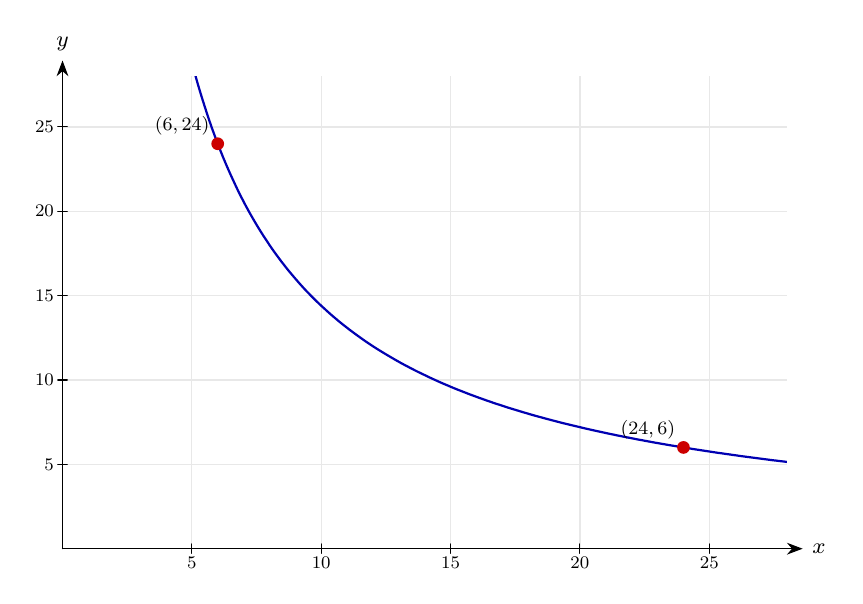
\begin{tikzpicture}[>={Stealth[length=2mm]},font=\footnotesize,line cap=round,line join=round]
\begin{scope}
\clip (0,0) rectangle (9.2,6);
\draw[gray!18] (0,0) grid[xstep=1.643,ystep=1.071] (9.2,6);
\draw[blue!70!black,thick] (0.023,12) -- (0.069,12) -- (0.115,12) -- (0.161,12) -- (0.207,12) -- (0.252,12) -- (0.298,12) -- (0.344,12) -- (0.39,12) -- (0.436,12) -- (0.482,12) -- (0.528,12) -- (0.574,12) -- (0.62,12) -- (0.665,12) -- (0.711,12) -- (0.757,12) -- (0.803,12) -- (0.849,11.943) -- (0.895,11.331) -- (0.941,10.778) -- (0.987,10.277) -- (1.032,9.82) -- (1.078,9.402) -- (1.124,9.018) -- (1.17,8.665) -- (1.216,8.338) -- (1.262,8.035) -- (1.308,7.753) -- (1.354,7.49) -- (1.4,7.244) -- (1.445,7.014) -- (1.491,6.799) -- (1.537,6.596) -- (1.583,6.404) -- (1.629,6.224) -- (1.675,6.054) -- (1.721,5.892) -- (1.767,5.739) -- (1.813,5.594) -- (1.858,5.456) -- (1.904,5.324) -- (1.95,5.199) -- (1.996,5.079) -- (2.042,4.965) -- (2.088,4.856) -- (2.134,4.752) -- (2.18,4.652) -- (2.225,4.556) -- (2.271,4.464) -- (2.317,4.375) -- (2.363,4.29) -- (2.409,4.209) -- (2.455,4.13) -- (2.501,4.054) -- (2.547,3.981) -- (2.593,3.911) -- (2.638,3.843) -- (2.684,3.777) -- (2.73,3.714) -- (2.776,3.652) -- (2.822,3.593) -- (2.868,3.535) -- (2.914,3.48) -- (2.96,3.426) -- (3.006,3.373) -- (3.051,3.323) -- (3.097,3.273) -- (3.143,3.226) -- (3.189,3.179) -- (3.235,3.134) -- (3.281,3.09) -- (3.327,3.048) -- (3.373,3.006) -- (3.418,2.966) -- (3.464,2.927) -- (3.51,2.888) -- (3.556,2.851) -- (3.602,2.815) -- (3.648,2.779) -- (3.694,2.745) -- (3.74,2.711) -- (3.786,2.678) -- (3.831,2.646) -- (3.877,2.615) -- (3.923,2.584) -- (3.969,2.554) -- (4.015,2.525) -- (4.061,2.497) -- (4.107,2.469) -- (4.153,2.442) -- (4.199,2.415) -- (4.244,2.389) -- (4.29,2.363) -- (4.336,2.338) -- (4.382,2.314) -- (4.428,2.29) -- (4.474,2.266) -- (4.52,2.243) -- (4.566,2.221) -- (4.612,2.199) -- (4.657,2.177) -- (4.703,2.156) -- (4.749,2.135) -- (4.795,2.114) -- (4.841,2.094) -- (4.887,2.075) -- (4.933,2.055) -- (4.979,2.036) -- (5.024,2.018) -- (5.07,2) -- (5.116,1.982) -- (5.162,1.964) -- (5.208,1.947) -- (5.254,1.93) -- (5.3,1.913) -- (5.346,1.897) -- (5.392,1.88) -- (5.437,1.865) -- (5.483,1.849) -- (5.529,1.834) -- (5.575,1.819) -- (5.621,1.804) -- (5.667,1.789) -- (5.713,1.775) -- (5.759,1.761) -- (5.805,1.747) -- (5.85,1.733) -- (5.896,1.72) -- (5.942,1.706) -- (5.988,1.693) -- (6.034,1.68) -- (6.08,1.668) -- (6.126,1.655) -- (6.172,1.643) -- (6.217,1.631) -- (6.263,1.619) -- (6.309,1.607) -- (6.355,1.595) -- (6.401,1.584) -- (6.447,1.573) -- (6.493,1.562) -- (6.539,1.551) -- (6.585,1.54) -- (6.63,1.529) -- (6.676,1.519) -- (6.722,1.508) -- (6.768,1.498) -- (6.814,1.488) -- (6.86,1.478) -- (6.906,1.468) -- (6.952,1.458) -- (6.998,1.449) -- (7.043,1.439) -- (7.089,1.43) -- (7.135,1.421) -- (7.181,1.412) -- (7.227,1.403) -- (7.273,1.394) -- (7.319,1.385) -- (7.365,1.377) -- (7.41,1.368) -- (7.456,1.36) -- (7.502,1.351) -- (7.548,1.343) -- (7.594,1.335) -- (7.64,1.327) -- (7.686,1.319) -- (7.732,1.311) -- (7.778,1.304) -- (7.823,1.296) -- (7.869,1.288) -- (7.915,1.281) -- (7.961,1.274) -- (8.007,1.266) -- (8.053,1.259) -- (8.099,1.252) -- (8.145,1.245) -- (8.191,1.238) -- (8.236,1.231) -- (8.282,1.224) -- (8.328,1.217) -- (8.374,1.211) -- (8.42,1.204) -- (8.466,1.198) -- (8.512,1.191) -- (8.558,1.185) -- (8.603,1.178) -- (8.649,1.172) -- (8.695,1.166) -- (8.741,1.16) -- (8.787,1.154) -- (8.833,1.148) -- (8.879,1.142) -- (8.925,1.136) -- (8.971,1.13) -- (9.016,1.124) -- (9.062,1.119) -- (9.108,1.113) -- (9.154,1.108) -- (9.2,1.102);
\end{scope}
\draw[->] (0,0) -- (9.4,0) node[right]{$x$};
\draw[->] (0,0) -- (0,6.2) node[above]{$y$};
\draw (1.643,-0.06) -- (1.643,0.06) node[below=2pt,scale=0.8]{$5$};
\draw (3.286,-0.06) -- (3.286,0.06) node[below=2pt,scale=0.8]{$10$};
\draw (4.929,-0.06) -- (4.929,0.06) node[below=2pt,scale=0.8]{$15$};
\draw (6.571,-0.06) -- (6.571,0.06) node[below=2pt,scale=0.8]{$20$};
\draw (8.214,-0.06) -- (8.214,0.06) node[below=2pt,scale=0.8]{$25$};
\draw (-0.06,1.071) -- (0.06,1.071) node[left=2pt,scale=0.8]{$5$};
\draw (-0.06,2.143) -- (0.06,2.143) node[left=2pt,scale=0.8]{$10$};
\draw (-0.06,3.214) -- (0.06,3.214) node[left=2pt,scale=0.8]{$15$};
\draw (-0.06,4.286) -- (0.06,4.286) node[left=2pt,scale=0.8]{$20$};
\draw (-0.06,5.357) -- (0.06,5.357) node[left=2pt,scale=0.8]{$25$};
\fill[red!80!black] (1.971,5.143) circle (2.3pt);
\node[above left,scale=0.85] at (1.971,5.143) {$(6,24)$};
\fill[red!80!black] (7.886,1.286) circle (2.3pt);
\node[above left,scale=0.85] at (7.886,1.286) {$(24,6)$};
\end{tikzpicture}
}
\end{center}
\small The relationship plotted, with the data points marked.\normalsize

\medskip\hrule

\section*{Proportion 15\quad\small\texttt{(cg4-015)}}
\addcontentsline{toc}{section}{Proportion 15 (cg4-015)}
\textit{Difficulty: Foundation \quad\textbar\quad Marks: 3}

\question{The volume \( V \) of a fixed mass of gas is inversely proportional to the pressure \( P \). When \( P = 250 \) Pa the volume is \( 4 \) m\textsuperscript{3}. Find the pressure when the volume is \( 2.5 \) m\textsuperscript{3}.}

\textbf{Worked solution.}

\textit{Step 1: Write \( V = \frac{k}{P} \) and find \( k \).}
\[\begin{gathered}
k = VP = 4 \times 250 = 1000
\end{gathered}\]
\( k \) is the constant product of volume and pressure.

\textit{Step 2: Substitute \( V = 2.5 \).}
\[\begin{gathered}
P = \frac{1000}{2.5} = 400 \text{ Pa}
\end{gathered}\]
Halving the volume doubles the pressure (approximately).

\begin{answerbox}
\textbf{Final answer:}\quad \(\displaystyle  P = 400 \) Pa
\end{answerbox}
\textbf{Graph.}

\begin{center}
\resizebox{\ifdim\width>\linewidth \linewidth\else \width\fi}{!}{%
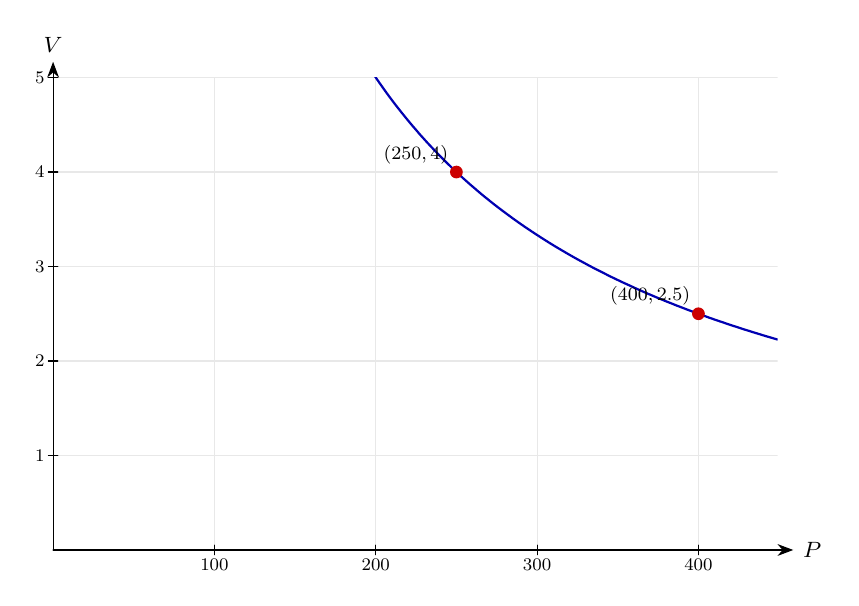
\begin{tikzpicture}[>={Stealth[length=2mm]},font=\footnotesize,line cap=round,line join=round]
\begin{scope}
\clip (0,0) rectangle (9.2,6);
\draw[gray!18] (0,0) grid[xstep=2.049,ystep=1.2] (9.2,6);
\draw[blue!70!black,thick] (0.023,12) -- (0.069,12) -- (0.115,12) -- (0.161,12) -- (0.207,12) -- (0.252,12) -- (0.298,12) -- (0.344,12) -- (0.39,12) -- (0.436,12) -- (0.482,12) -- (0.528,12) -- (0.574,12) -- (0.62,12) -- (0.665,12) -- (0.711,12) -- (0.757,12) -- (0.803,12) -- (0.849,12) -- (0.895,12) -- (0.941,12) -- (0.987,12) -- (1.032,12) -- (1.078,12) -- (1.124,12) -- (1.17,12) -- (1.216,12) -- (1.262,12) -- (1.308,12) -- (1.354,12) -- (1.4,12) -- (1.445,12) -- (1.491,12) -- (1.537,12) -- (1.583,12) -- (1.629,12) -- (1.675,12) -- (1.721,12) -- (1.767,12) -- (1.813,12) -- (1.858,12) -- (1.904,12) -- (1.95,12) -- (1.996,12) -- (2.042,12) -- (2.088,11.777) -- (2.134,11.524) -- (2.18,11.281) -- (2.225,11.048) -- (2.271,10.825) -- (2.317,10.611) -- (2.363,10.405) -- (2.409,10.207) -- (2.455,10.016) -- (2.501,9.832) -- (2.547,9.655) -- (2.593,9.484) -- (2.638,9.319) -- (2.684,9.16) -- (2.73,9.006) -- (2.776,8.857) -- (2.822,8.713) -- (2.868,8.574) -- (2.914,8.439) -- (2.96,8.308) -- (3.006,8.181) -- (3.051,8.058) -- (3.097,7.939) -- (3.143,7.823) -- (3.189,7.71) -- (3.235,7.601) -- (3.281,7.494) -- (3.327,7.391) -- (3.373,7.29) -- (3.418,7.193) -- (3.464,7.097) -- (3.51,7.005) -- (3.556,6.914) -- (3.602,6.826) -- (3.648,6.74) -- (3.694,6.657) -- (3.74,6.575) -- (3.786,6.495) -- (3.831,6.417) -- (3.877,6.341) -- (3.923,6.267) -- (3.969,6.195) -- (4.015,6.124) -- (4.061,6.055) -- (4.107,5.987) -- (4.153,5.921) -- (4.199,5.856) -- (4.244,5.793) -- (4.29,5.731) -- (4.336,5.67) -- (4.382,5.611) -- (4.428,5.553) -- (4.474,5.496) -- (4.52,5.44) -- (4.566,5.385) -- (4.612,5.332) -- (4.657,5.279) -- (4.703,5.228) -- (4.749,5.177) -- (4.795,5.128) -- (4.841,5.079) -- (4.887,5.031) -- (4.933,4.985) -- (4.979,4.939) -- (5.024,4.894) -- (5.07,4.849) -- (5.116,4.806) -- (5.162,4.763) -- (5.208,4.721) -- (5.254,4.68) -- (5.3,4.639) -- (5.346,4.6) -- (5.392,4.56) -- (5.437,4.522) -- (5.483,4.484) -- (5.529,4.447) -- (5.575,4.41) -- (5.621,4.374) -- (5.667,4.339) -- (5.713,4.304) -- (5.759,4.27) -- (5.805,4.236) -- (5.85,4.203) -- (5.896,4.17) -- (5.942,4.138) -- (5.988,4.106) -- (6.034,4.075) -- (6.08,4.044) -- (6.126,4.014) -- (6.172,3.984) -- (6.217,3.955) -- (6.263,3.926) -- (6.309,3.897) -- (6.355,3.869) -- (6.401,3.841) -- (6.447,3.814) -- (6.493,3.787) -- (6.539,3.76) -- (6.585,3.734) -- (6.63,3.708) -- (6.676,3.683) -- (6.722,3.658) -- (6.768,3.633) -- (6.814,3.608) -- (6.86,3.584) -- (6.906,3.561) -- (6.952,3.537) -- (6.998,3.514) -- (7.043,3.491) -- (7.089,3.468) -- (7.135,3.446) -- (7.181,3.424) -- (7.227,3.402) -- (7.273,3.381) -- (7.319,3.36) -- (7.365,3.339) -- (7.41,3.318) -- (7.456,3.298) -- (7.502,3.277) -- (7.548,3.257) -- (7.594,3.238) -- (7.64,3.218) -- (7.686,3.199) -- (7.732,3.18) -- (7.778,3.161) -- (7.823,3.143) -- (7.869,3.125) -- (7.915,3.106) -- (7.961,3.089) -- (8.007,3.071) -- (8.053,3.053) -- (8.099,3.036) -- (8.145,3.019) -- (8.191,3.002) -- (8.236,2.985) -- (8.282,2.969) -- (8.328,2.952) -- (8.374,2.936) -- (8.42,2.92) -- (8.466,2.904) -- (8.512,2.889) -- (8.558,2.873) -- (8.603,2.858) -- (8.649,2.843) -- (8.695,2.828) -- (8.741,2.813) -- (8.787,2.798) -- (8.833,2.784) -- (8.879,2.769) -- (8.925,2.755) -- (8.971,2.741) -- (9.016,2.727) -- (9.062,2.713) -- (9.108,2.7) -- (9.154,2.686) -- (9.2,2.673);
\end{scope}
\draw[->] (0,0) -- (9.4,0) node[right]{$P$};
\draw[->] (0,0) -- (0,6.2) node[above]{$V$};
\draw (2.049,-0.06) -- (2.049,0.06) node[below=2pt,scale=0.8]{$100$};
\draw (4.098,-0.06) -- (4.098,0.06) node[below=2pt,scale=0.8]{$200$};
\draw (6.147,-0.06) -- (6.147,0.06) node[below=2pt,scale=0.8]{$300$};
\draw (8.196,-0.06) -- (8.196,0.06) node[below=2pt,scale=0.8]{$400$};
\draw (-0.06,1.2) -- (0.06,1.2) node[left=2pt,scale=0.8]{$1$};
\draw (-0.06,2.4) -- (0.06,2.4) node[left=2pt,scale=0.8]{$2$};
\draw (-0.06,3.6) -- (0.06,3.6) node[left=2pt,scale=0.8]{$3$};
\draw (-0.06,4.8) -- (0.06,4.8) node[left=2pt,scale=0.8]{$4$};
\draw (-0.06,6) -- (0.06,6) node[left=2pt,scale=0.8]{$5$};
\fill[red!80!black] (5.122,4.8) circle (2.3pt);
\node[above left,scale=0.85] at (5.122,4.8) {$(250,4)$};
\fill[red!80!black] (8.196,3) circle (2.3pt);
\node[above left,scale=0.85] at (8.196,3) {$(400,2.5)$};
\end{tikzpicture}
}
\end{center}
\small The relationship plotted, with the data points marked.\normalsize

\medskip\hrule

\section*{Proportion 16\quad\small\texttt{(cg4-016)}}
\addcontentsline{toc}{section}{Proportion 16 (cg4-016)}
\textit{Difficulty: Foundation \quad\textbar\quad Marks: 3}

\question{Given that \( y \propto x^2 \) and that \( y = 75 \) when \( x = 5 \), find \( y \) when \( x = 4 \).}

\textbf{Worked solution.}

\textit{Step 1: Write \( y = kx^2 \) and substitute.}
\[\begin{gathered}
75 = k \times 25 \implies k = 3
\end{gathered}\]
Divide both sides by \( 5^2 = 25 \).

\textit{Step 2: Substitute \( x = 4 \).}
\[\begin{gathered}
y = 3 \times 16 = 48
\end{gathered}\]
Square \( x \) first, then multiply by \( k \).

\begin{answerbox}
\textbf{Final answer:}\quad \(\displaystyle  y = 48 \)
\end{answerbox}
\textbf{Graph.}

\begin{center}
\resizebox{\ifdim\width>\linewidth \linewidth\else \width\fi}{!}{%
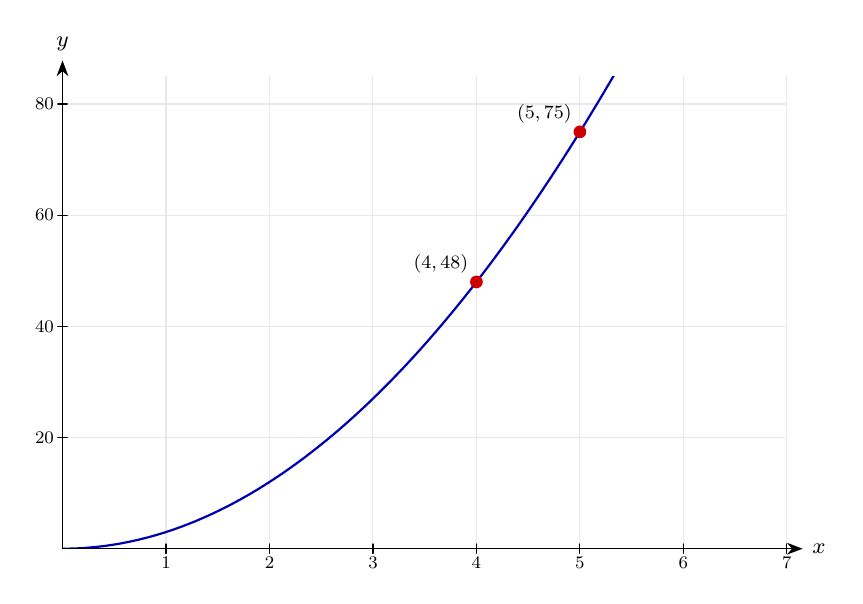
\begin{tikzpicture}[>={Stealth[length=2mm]},font=\footnotesize,line cap=round,line join=round]
\begin{scope}
\clip (0,0) rectangle (9.2,6);
\draw[gray!18] (0,0) grid[xstep=1.314,ystep=1.412] (9.2,6);
\draw[blue!70!black,thick] (0,0) -- (0.046,0) -- (0.092,0.001) -- (0.138,0.002) -- (0.184,0.004) -- (0.23,0.006) -- (0.276,0.009) -- (0.322,0.013) -- (0.368,0.017) -- (0.414,0.021) -- (0.46,0.026) -- (0.506,0.031) -- (0.552,0.037) -- (0.598,0.044) -- (0.644,0.051) -- (0.69,0.058) -- (0.736,0.066) -- (0.782,0.075) -- (0.828,0.084) -- (0.874,0.094) -- (0.92,0.104) -- (0.966,0.114) -- (1.012,0.126) -- (1.058,0.137) -- (1.104,0.149) -- (1.15,0.162) -- (1.196,0.175) -- (1.242,0.189) -- (1.288,0.203) -- (1.334,0.218) -- (1.38,0.233) -- (1.426,0.249) -- (1.472,0.266) -- (1.518,0.282) -- (1.564,0.3) -- (1.61,0.318) -- (1.656,0.336) -- (1.702,0.355) -- (1.748,0.375) -- (1.794,0.395) -- (1.84,0.415) -- (1.886,0.436) -- (1.932,0.458) -- (1.978,0.48) -- (2.024,0.502) -- (2.07,0.525) -- (2.116,0.549) -- (2.162,0.573) -- (2.208,0.598) -- (2.254,0.623) -- (2.3,0.649) -- (2.346,0.675) -- (2.392,0.701) -- (2.438,0.729) -- (2.484,0.756) -- (2.53,0.785) -- (2.576,0.814) -- (2.622,0.843) -- (2.668,0.873) -- (2.714,0.903) -- (2.76,0.934) -- (2.806,0.965) -- (2.852,0.997) -- (2.898,1.03) -- (2.944,1.063) -- (2.99,1.096) -- (3.036,1.13) -- (3.082,1.164) -- (3.128,1.2) -- (3.174,1.235) -- (3.22,1.271) -- (3.266,1.308) -- (3.312,1.345) -- (3.358,1.382) -- (3.404,1.421) -- (3.45,1.459) -- (3.496,1.498) -- (3.542,1.538) -- (3.588,1.578) -- (3.634,1.619) -- (3.68,1.66) -- (3.726,1.702) -- (3.772,1.744) -- (3.818,1.787) -- (3.864,1.83) -- (3.91,1.874) -- (3.956,1.919) -- (4.002,1.963) -- (4.048,2.009) -- (4.094,2.055) -- (4.14,2.101) -- (4.186,2.148) -- (4.232,2.196) -- (4.278,2.244) -- (4.324,2.292) -- (4.37,2.341) -- (4.416,2.391) -- (4.462,2.441) -- (4.508,2.491) -- (4.554,2.542) -- (4.6,2.594) -- (4.646,2.646) -- (4.692,2.699) -- (4.738,2.752) -- (4.784,2.806) -- (4.83,2.86) -- (4.876,2.915) -- (4.922,2.97) -- (4.968,3.026) -- (5.014,3.082) -- (5.06,3.139) -- (5.106,3.196) -- (5.152,3.254) -- (5.198,3.312) -- (5.244,3.371) -- (5.29,3.431) -- (5.336,3.491) -- (5.382,3.551) -- (5.428,3.612) -- (5.474,3.674) -- (5.52,3.736) -- (5.566,3.798) -- (5.612,3.861) -- (5.658,3.925) -- (5.704,3.989) -- (5.75,4.053) -- (5.796,4.118) -- (5.842,4.184) -- (5.888,4.25) -- (5.934,4.317) -- (5.98,4.384) -- (6.026,4.452) -- (6.072,4.52) -- (6.118,4.589) -- (6.164,4.658) -- (6.21,4.728) -- (6.256,4.798) -- (6.302,4.869) -- (6.348,4.94) -- (6.394,5.012) -- (6.44,5.084) -- (6.486,5.157) -- (6.532,5.231) -- (6.578,5.305) -- (6.624,5.379) -- (6.67,5.454) -- (6.716,5.53) -- (6.762,5.606) -- (6.808,5.682) -- (6.854,5.759) -- (6.9,5.837) -- (6.946,5.915) -- (6.992,5.993) -- (7.038,6.073) -- (7.084,6.152) -- (7.13,6.232) -- (7.176,6.313) -- (7.222,6.394) -- (7.268,6.476) -- (7.314,6.558) -- (7.36,6.641) -- (7.406,6.724) -- (7.452,6.808) -- (7.498,6.892) -- (7.544,6.977) -- (7.59,7.062) -- (7.636,7.148) -- (7.682,7.235) -- (7.728,7.322) -- (7.774,7.409) -- (7.82,7.497) -- (7.866,7.585) -- (7.912,7.674) -- (7.958,7.764) -- (8.004,7.854) -- (8.05,7.944) -- (8.096,8.036) -- (8.142,8.127) -- (8.188,8.219) -- (8.234,8.312) -- (8.28,8.405) -- (8.326,8.499) -- (8.372,8.593) -- (8.418,8.687) -- (8.464,8.783) -- (8.51,8.878) -- (8.556,8.975) -- (8.602,9.071) -- (8.648,9.169) -- (8.694,9.266) -- (8.74,9.365) -- (8.786,9.464) -- (8.832,9.563) -- (8.878,9.663) -- (8.924,9.763) -- (8.97,9.864) -- (9.016,9.966) -- (9.062,10.068) -- (9.108,10.17) -- (9.154,10.273) -- (9.2,10.376);
\end{scope}
\draw[->] (0,0) -- (9.4,0) node[right]{$x$};
\draw[->] (0,0) -- (0,6.2) node[above]{$y$};
\draw (1.314,-0.06) -- (1.314,0.06) node[below=2pt,scale=0.8]{$1$};
\draw (2.629,-0.06) -- (2.629,0.06) node[below=2pt,scale=0.8]{$2$};
\draw (3.943,-0.06) -- (3.943,0.06) node[below=2pt,scale=0.8]{$3$};
\draw (5.257,-0.06) -- (5.257,0.06) node[below=2pt,scale=0.8]{$4$};
\draw (6.571,-0.06) -- (6.571,0.06) node[below=2pt,scale=0.8]{$5$};
\draw (7.886,-0.06) -- (7.886,0.06) node[below=2pt,scale=0.8]{$6$};
\draw (9.2,-0.06) -- (9.2,0.06) node[below=2pt,scale=0.8]{$7$};
\draw (-0.06,1.412) -- (0.06,1.412) node[left=2pt,scale=0.8]{$20$};
\draw (-0.06,2.824) -- (0.06,2.824) node[left=2pt,scale=0.8]{$40$};
\draw (-0.06,4.235) -- (0.06,4.235) node[left=2pt,scale=0.8]{$60$};
\draw (-0.06,5.647) -- (0.06,5.647) node[left=2pt,scale=0.8]{$80$};
\fill[red!80!black] (6.571,5.294) circle (2.3pt);
\node[above left,scale=0.85] at (6.571,5.294) {$(5,75)$};
\fill[red!80!black] (5.257,3.388) circle (2.3pt);
\node[above left,scale=0.85] at (5.257,3.388) {$(4,48)$};
\end{tikzpicture}
}
\end{center}
\small The relationship plotted, with the data points marked.\normalsize

\medskip\hrule

\section*{Proportion 17\quad\small\texttt{(cg4-017)}}
\addcontentsline{toc}{section}{Proportion 17 (cg4-017)}
\textit{Difficulty: Foundation \quad\textbar\quad Marks: 3}

\question{The surface area \( A \) cm\textsuperscript{2} of a sphere is directly proportional to the square of its radius \( r \) cm. When \( r = 3 \), \( A = 36\pi \). Find \( A \) when \( r = 5 \).}

\textbf{Worked solution.}

\textit{Step 1: Write \( A = kr^2 \) and substitute \( r=3, A=36\pi \).}
\[\begin{gathered}
36\pi = k \times 9 \implies k = 4\pi
\end{gathered}\]
Divide both sides by 9.

\textit{Step 2: Substitute \( r = 5 \).}
\[\begin{gathered}
A = 4\pi \times 25 = 100\pi \text{ cm}^2
\end{gathered}\]
The surface area of a sphere is indeed \( 4\pi r^2 \).

\begin{answerbox}
\textbf{Final answer:}\quad \(\displaystyle  A = 100\pi \) cm\textsuperscript{2}
\end{answerbox}
\textbf{Graph.}

\begin{center}
\resizebox{\ifdim\width>\linewidth \linewidth\else \width\fi}{!}{%
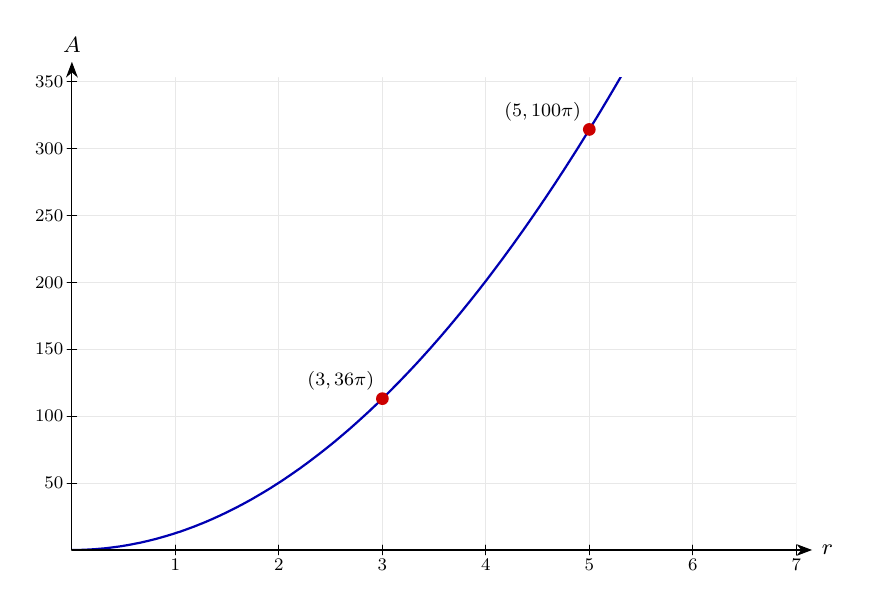
\begin{tikzpicture}[>={Stealth[length=2mm]},font=\footnotesize,line cap=round,line join=round]
\begin{scope}
\clip (0,0) rectangle (9.2,6);
\draw[gray!18] (0,0) grid[xstep=1.314,ystep=0.85] (9.2,6);
\draw[blue!70!black,thick] (0,0) -- (0.046,0) -- (0.092,0.001) -- (0.138,0.002) -- (0.184,0.004) -- (0.23,0.007) -- (0.276,0.009) -- (0.322,0.013) -- (0.368,0.017) -- (0.414,0.021) -- (0.46,0.026) -- (0.506,0.032) -- (0.552,0.038) -- (0.598,0.044) -- (0.644,0.051) -- (0.69,0.059) -- (0.736,0.067) -- (0.782,0.076) -- (0.828,0.085) -- (0.874,0.094) -- (0.92,0.105) -- (0.966,0.115) -- (1.012,0.127) -- (1.058,0.138) -- (1.104,0.151) -- (1.15,0.164) -- (1.196,0.177) -- (1.242,0.191) -- (1.288,0.205) -- (1.334,0.22) -- (1.38,0.235) -- (1.426,0.251) -- (1.472,0.268) -- (1.518,0.285) -- (1.564,0.302) -- (1.61,0.321) -- (1.656,0.339) -- (1.702,0.358) -- (1.748,0.378) -- (1.794,0.398) -- (1.84,0.419) -- (1.886,0.44) -- (1.932,0.462) -- (1.978,0.484) -- (2.024,0.507) -- (2.07,0.53) -- (2.116,0.554) -- (2.162,0.578) -- (2.208,0.603) -- (2.254,0.628) -- (2.3,0.654) -- (2.346,0.681) -- (2.392,0.708) -- (2.438,0.735) -- (2.484,0.763) -- (2.53,0.791) -- (2.576,0.821) -- (2.622,0.85) -- (2.668,0.88) -- (2.714,0.911) -- (2.76,0.942) -- (2.806,0.974) -- (2.852,1.006) -- (2.898,1.038) -- (2.944,1.072) -- (2.99,1.105) -- (3.036,1.14) -- (3.082,1.175) -- (3.128,1.21) -- (3.174,1.246) -- (3.22,1.282) -- (3.266,1.319) -- (3.312,1.356) -- (3.358,1.394) -- (3.404,1.433) -- (3.45,1.472) -- (3.496,1.511) -- (3.542,1.551) -- (3.588,1.592) -- (3.634,1.633) -- (3.68,1.675) -- (3.726,1.717) -- (3.772,1.759) -- (3.818,1.803) -- (3.864,1.846) -- (3.91,1.89) -- (3.956,1.935) -- (4.002,1.98) -- (4.048,2.026) -- (4.094,2.073) -- (4.14,2.119) -- (4.186,2.167) -- (4.232,2.215) -- (4.278,2.263) -- (4.324,2.312) -- (4.37,2.361) -- (4.416,2.411) -- (4.462,2.462) -- (4.508,2.513) -- (4.554,2.564) -- (4.6,2.617) -- (4.646,2.669) -- (4.692,2.722) -- (4.738,2.776) -- (4.784,2.83) -- (4.83,2.885) -- (4.876,2.94) -- (4.922,2.996) -- (4.968,3.052) -- (5.014,3.109) -- (5.06,3.166) -- (5.106,3.224) -- (5.152,3.282) -- (5.198,3.341) -- (5.244,3.4) -- (5.29,3.46) -- (5.336,3.521) -- (5.382,3.582) -- (5.428,3.643) -- (5.474,3.705) -- (5.52,3.768) -- (5.566,3.831) -- (5.612,3.894) -- (5.658,3.959) -- (5.704,4.023) -- (5.75,4.088) -- (5.796,4.154) -- (5.842,4.22) -- (5.888,4.287) -- (5.934,4.354) -- (5.98,4.422) -- (6.026,4.49) -- (6.072,4.559) -- (6.118,4.628) -- (6.164,4.698) -- (6.21,4.769) -- (6.256,4.839) -- (6.302,4.911) -- (6.348,4.983) -- (6.394,5.055) -- (6.44,5.128) -- (6.486,5.202) -- (6.532,5.276) -- (6.578,5.351) -- (6.624,5.426) -- (6.67,5.501) -- (6.716,5.577) -- (6.762,5.654) -- (6.808,5.731) -- (6.854,5.809) -- (6.9,5.887) -- (6.946,5.966) -- (6.992,6.045) -- (7.038,6.125) -- (7.084,6.205) -- (7.13,6.286) -- (7.176,6.368) -- (7.222,6.449) -- (7.268,6.532) -- (7.314,6.615) -- (7.36,6.698) -- (7.406,6.782) -- (7.452,6.867) -- (7.498,6.952) -- (7.544,7.037) -- (7.59,7.123) -- (7.636,7.21) -- (7.682,7.297) -- (7.728,7.385) -- (7.774,7.473) -- (7.82,7.562) -- (7.866,7.651) -- (7.912,7.741) -- (7.958,7.831) -- (8.004,7.922) -- (8.05,8.013) -- (8.096,8.105) -- (8.142,8.197) -- (8.188,8.29) -- (8.234,8.384) -- (8.28,8.477) -- (8.326,8.572) -- (8.372,8.667) -- (8.418,8.762) -- (8.464,8.858) -- (8.51,8.955) -- (8.556,9.052) -- (8.602,9.15) -- (8.648,9.248) -- (8.694,9.346) -- (8.74,9.446) -- (8.786,9.545) -- (8.832,9.646) -- (8.878,9.746) -- (8.924,9.847) -- (8.97,9.949) -- (9.016,10.052) -- (9.062,10.154) -- (9.108,10.258) -- (9.154,10.362) -- (9.2,10.466);
\end{scope}
\draw[->] (0,0) -- (9.4,0) node[right]{$r$};
\draw[->] (0,0) -- (0,6.2) node[above]{$A$};
\draw (1.314,-0.06) -- (1.314,0.06) node[below=2pt,scale=0.8]{$1$};
\draw (2.629,-0.06) -- (2.629,0.06) node[below=2pt,scale=0.8]{$2$};
\draw (3.943,-0.06) -- (3.943,0.06) node[below=2pt,scale=0.8]{$3$};
\draw (5.257,-0.06) -- (5.257,0.06) node[below=2pt,scale=0.8]{$4$};
\draw (6.571,-0.06) -- (6.571,0.06) node[below=2pt,scale=0.8]{$5$};
\draw (7.886,-0.06) -- (7.886,0.06) node[below=2pt,scale=0.8]{$6$};
\draw (9.2,-0.06) -- (9.2,0.06) node[below=2pt,scale=0.8]{$7$};
\draw (-0.06,0.85) -- (0.06,0.85) node[left=2pt,scale=0.8]{$50$};
\draw (-0.06,1.7) -- (0.06,1.7) node[left=2pt,scale=0.8]{$100$};
\draw (-0.06,2.55) -- (0.06,2.55) node[left=2pt,scale=0.8]{$150$};
\draw (-0.06,3.399) -- (0.06,3.399) node[left=2pt,scale=0.8]{$200$};
\draw (-0.06,4.249) -- (0.06,4.249) node[left=2pt,scale=0.8]{$250$};
\draw (-0.06,5.099) -- (0.06,5.099) node[left=2pt,scale=0.8]{$300$};
\draw (-0.06,5.949) -- (0.06,5.949) node[left=2pt,scale=0.8]{$350$};
\fill[red!80!black] (3.943,1.922) circle (2.3pt);
\node[above left,scale=0.85] at (3.943,1.922) {$(3,36\pi)$};
\fill[red!80!black] (6.571,5.341) circle (2.3pt);
\node[above left,scale=0.85] at (6.571,5.341) {$(5,100\pi)$};
\end{tikzpicture}
}
\end{center}
\small The relationship plotted, with the data points marked.\normalsize

\medskip\hrule

\section*{Proportion 18\quad\small\texttt{(cg4-018)}}
\addcontentsline{toc}{section}{Proportion 18 (cg4-018)}
\textit{Difficulty: Foundation \quad\textbar\quad Marks: 4}

\question{Given that \( y \propto x^2 \) and \( y = 20 \) when \( x = 2 \), find the value of \( x \) (with \( x > 0 \)) when \( y = 125 \).}

\textbf{Worked solution.}

\textit{Step 1: Find \( k \).}
\[\begin{gathered}
20 = k \times 4 \implies k = 5
\end{gathered}\]
Divide both sides by \( 2^2 = 4 \).

\textit{Step 2: Substitute \( y = 125 \).}
\[\begin{gathered}
125 = 5x^2 \implies x^2 = 25
\end{gathered}\]
Divide both sides by 5.

\textit{Step 3: Take the positive square root.}
\[\begin{gathered}
x = 5
\end{gathered}\]
Since \( x > 0 \), take the positive root only.

\begin{answerbox}
\textbf{Final answer:}\quad \(\displaystyle  x = 5 \)
\end{answerbox}
\textbf{Graph.}

\begin{center}
\resizebox{\ifdim\width>\linewidth \linewidth\else \width\fi}{!}{%
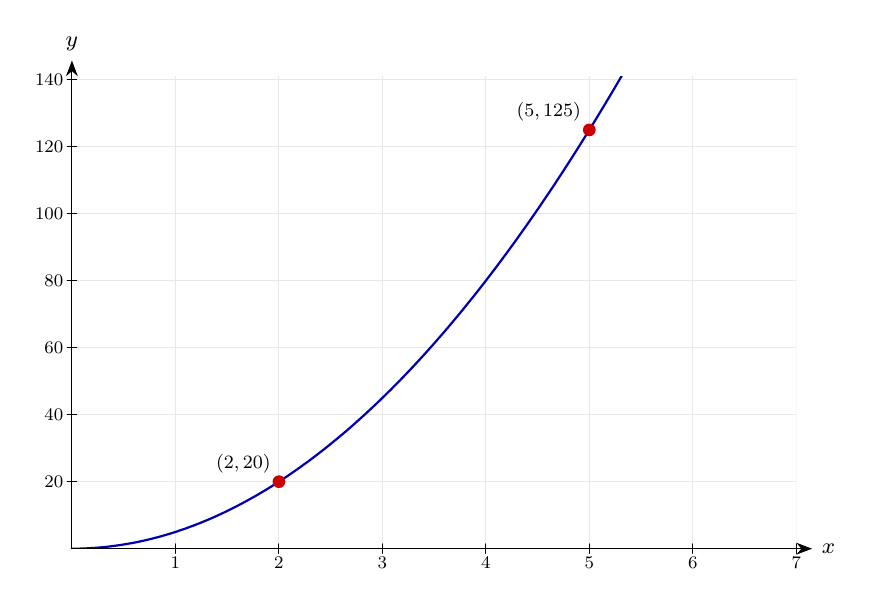
\begin{tikzpicture}[>={Stealth[length=2mm]},font=\footnotesize,line cap=round,line join=round]
\begin{scope}
\clip (0,0) rectangle (9.2,6);
\draw[gray!18] (0,0) grid[xstep=1.314,ystep=0.851] (9.2,6);
\draw[blue!70!black,thick] (0,0) -- (0.046,0) -- (0.092,0.001) -- (0.138,0.002) -- (0.184,0.004) -- (0.23,0.007) -- (0.276,0.009) -- (0.322,0.013) -- (0.368,0.017) -- (0.414,0.021) -- (0.46,0.026) -- (0.506,0.032) -- (0.552,0.038) -- (0.598,0.044) -- (0.644,0.051) -- (0.69,0.059) -- (0.736,0.067) -- (0.782,0.075) -- (0.828,0.084) -- (0.874,0.094) -- (0.92,0.104) -- (0.966,0.115) -- (1.012,0.126) -- (1.058,0.138) -- (1.104,0.15) -- (1.15,0.163) -- (1.196,0.176) -- (1.242,0.19) -- (1.288,0.204) -- (1.334,0.219) -- (1.38,0.235) -- (1.426,0.25) -- (1.472,0.267) -- (1.518,0.284) -- (1.564,0.301) -- (1.61,0.319) -- (1.656,0.338) -- (1.702,0.357) -- (1.748,0.376) -- (1.794,0.396) -- (1.84,0.417) -- (1.886,0.438) -- (1.932,0.46) -- (1.978,0.482) -- (2.024,0.505) -- (2.07,0.528) -- (2.116,0.552) -- (2.162,0.576) -- (2.208,0.601) -- (2.254,0.626) -- (2.3,0.652) -- (2.346,0.678) -- (2.392,0.705) -- (2.438,0.732) -- (2.484,0.76) -- (2.53,0.788) -- (2.576,0.817) -- (2.622,0.847) -- (2.668,0.877) -- (2.714,0.907) -- (2.76,0.938) -- (2.806,0.97) -- (2.852,1.002) -- (2.898,1.034) -- (2.944,1.068) -- (2.99,1.101) -- (3.036,1.135) -- (3.082,1.17) -- (3.128,1.205) -- (3.174,1.241) -- (3.22,1.277) -- (3.266,1.314) -- (3.312,1.351) -- (3.358,1.389) -- (3.404,1.427) -- (3.45,1.466) -- (3.496,1.505) -- (3.542,1.545) -- (3.588,1.586) -- (3.634,1.627) -- (3.68,1.668) -- (3.726,1.71) -- (3.772,1.753) -- (3.818,1.796) -- (3.864,1.839) -- (3.91,1.883) -- (3.956,1.928) -- (4.002,1.973) -- (4.048,2.018) -- (4.094,2.065) -- (4.14,2.111) -- (4.186,2.158) -- (4.232,2.206) -- (4.278,2.254) -- (4.324,2.303) -- (4.37,2.352) -- (4.416,2.402) -- (4.462,2.452) -- (4.508,2.503) -- (4.554,2.555) -- (4.6,2.606) -- (4.646,2.659) -- (4.692,2.712) -- (4.738,2.765) -- (4.784,2.819) -- (4.83,2.874) -- (4.876,2.929) -- (4.922,2.984) -- (4.968,3.04) -- (5.014,3.097) -- (5.06,3.154) -- (5.106,3.211) -- (5.152,3.269) -- (5.198,3.328) -- (5.244,3.387) -- (5.29,3.447) -- (5.336,3.507) -- (5.382,3.568) -- (5.428,3.629) -- (5.474,3.691) -- (5.52,3.753) -- (5.566,3.816) -- (5.612,3.879) -- (5.658,3.943) -- (5.704,4.008) -- (5.75,4.072) -- (5.796,4.138) -- (5.842,4.204) -- (5.888,4.27) -- (5.934,4.337) -- (5.98,4.405) -- (6.026,4.473) -- (6.072,4.541) -- (6.118,4.61) -- (6.164,4.68) -- (6.21,4.75) -- (6.256,4.821) -- (6.302,4.892) -- (6.348,4.964) -- (6.394,5.036) -- (6.44,5.109) -- (6.486,5.182) -- (6.532,5.256) -- (6.578,5.33) -- (6.624,5.405) -- (6.67,5.48) -- (6.716,5.556) -- (6.762,5.632) -- (6.808,5.709) -- (6.854,5.786) -- (6.9,5.864) -- (6.946,5.943) -- (6.992,6.022) -- (7.038,6.101) -- (7.084,6.181) -- (7.13,6.262) -- (7.176,6.343) -- (7.222,6.424) -- (7.268,6.507) -- (7.314,6.589) -- (7.36,6.672) -- (7.406,6.756) -- (7.452,6.84) -- (7.498,6.925) -- (7.544,7.01) -- (7.59,7.096) -- (7.636,7.182) -- (7.682,7.269) -- (7.728,7.356) -- (7.774,7.444) -- (7.82,7.532) -- (7.866,7.621) -- (7.912,7.711) -- (7.958,7.801) -- (8.004,7.891) -- (8.05,7.982) -- (8.096,8.074) -- (8.142,8.166) -- (8.188,8.258) -- (8.234,8.351) -- (8.28,8.445) -- (8.326,8.539) -- (8.372,8.633) -- (8.418,8.729) -- (8.464,8.824) -- (8.51,8.92) -- (8.556,9.017) -- (8.602,9.114) -- (8.648,9.212) -- (8.694,9.31) -- (8.74,9.409) -- (8.786,9.508) -- (8.832,9.608) -- (8.878,9.709) -- (8.924,9.809) -- (8.97,9.911) -- (9.016,10.013) -- (9.062,10.115) -- (9.108,10.218) -- (9.154,10.322) -- (9.2,10.426);
\end{scope}
\draw[->] (0,0) -- (9.4,0) node[right]{$x$};
\draw[->] (0,0) -- (0,6.2) node[above]{$y$};
\draw (1.314,-0.06) -- (1.314,0.06) node[below=2pt,scale=0.8]{$1$};
\draw (2.629,-0.06) -- (2.629,0.06) node[below=2pt,scale=0.8]{$2$};
\draw (3.943,-0.06) -- (3.943,0.06) node[below=2pt,scale=0.8]{$3$};
\draw (5.257,-0.06) -- (5.257,0.06) node[below=2pt,scale=0.8]{$4$};
\draw (6.571,-0.06) -- (6.571,0.06) node[below=2pt,scale=0.8]{$5$};
\draw (7.886,-0.06) -- (7.886,0.06) node[below=2pt,scale=0.8]{$6$};
\draw (9.2,-0.06) -- (9.2,0.06) node[below=2pt,scale=0.8]{$7$};
\draw (-0.06,0.851) -- (0.06,0.851) node[left=2pt,scale=0.8]{$20$};
\draw (-0.06,1.702) -- (0.06,1.702) node[left=2pt,scale=0.8]{$40$};
\draw (-0.06,2.553) -- (0.06,2.553) node[left=2pt,scale=0.8]{$60$};
\draw (-0.06,3.404) -- (0.06,3.404) node[left=2pt,scale=0.8]{$80$};
\draw (-0.06,4.255) -- (0.06,4.255) node[left=2pt,scale=0.8]{$100$};
\draw (-0.06,5.106) -- (0.06,5.106) node[left=2pt,scale=0.8]{$120$};
\draw (-0.06,5.957) -- (0.06,5.957) node[left=2pt,scale=0.8]{$140$};
\fill[red!80!black] (2.629,0.851) circle (2.3pt);
\node[above left,scale=0.85] at (2.629,0.851) {$(2,20)$};
\fill[red!80!black] (6.571,5.319) circle (2.3pt);
\node[above left,scale=0.85] at (6.571,5.319) {$(5,125)$};
\end{tikzpicture}
}
\end{center}
\small The relationship plotted, with the data points marked.\normalsize

\medskip\hrule

\section*{Proportion 19\quad\small\texttt{(cg4-019)}}
\addcontentsline{toc}{section}{Proportion 19 (cg4-019)}
\textit{Difficulty: Foundation \quad\textbar\quad Marks: 6}

\question{The braking distance \( d \) metres of a car is directly proportional to the square of its speed \( v \) km/h. At 30 km/h the braking distance is 9 m. \\[3pt] a) Find the equation connecting \( d \) and \( v \). \\[3pt] b) Find the braking distance at 50 km/h. \\[3pt] c) Find the speed at which the braking distance is 36 m.}

\textbf{Worked solution.}

\textit{Step 1: Write \( d = kv^2 \) and find \( k \).}
\[\begin{gathered}
9 = k \times 900 \implies k = \frac{9}{900} = \frac{1}{100}
\end{gathered}\]
Substitute \( d=9, v=30 \) and divide.

\textit{Step 2: Part a: state the equation.}
\[\begin{gathered}
d = \frac{v^2}{100}
\end{gathered}\]
This is the proportionality equation.

\textit{Step 3: Part b: substitute \( v = 50 \).}
\[\begin{gathered}
d = \frac{2500}{100} = 25 \text{ m}
\end{gathered}\]
The braking distance is 25 m at 50 km/h.

\textit{Step 4: Part c: substitute \( d = 36 \) and solve.}
\[\begin{gathered}
36 = \frac{v^2}{100} \implies v^2 = 3600 \implies v = 60 \text{ km/h}
\end{gathered}\]
Take the positive square root (speed is positive).

\begin{answerbox}
\textbf{Final answer:}\quad a) \(\displaystyle d = \frac{v^2}{100}\); b) \(\displaystyle 25\) m; c) \(\displaystyle 60\) km/h
\end{answerbox}
\textbf{Graph.}

\begin{center}
\resizebox{\ifdim\width>\linewidth \linewidth\else \width\fi}{!}{%
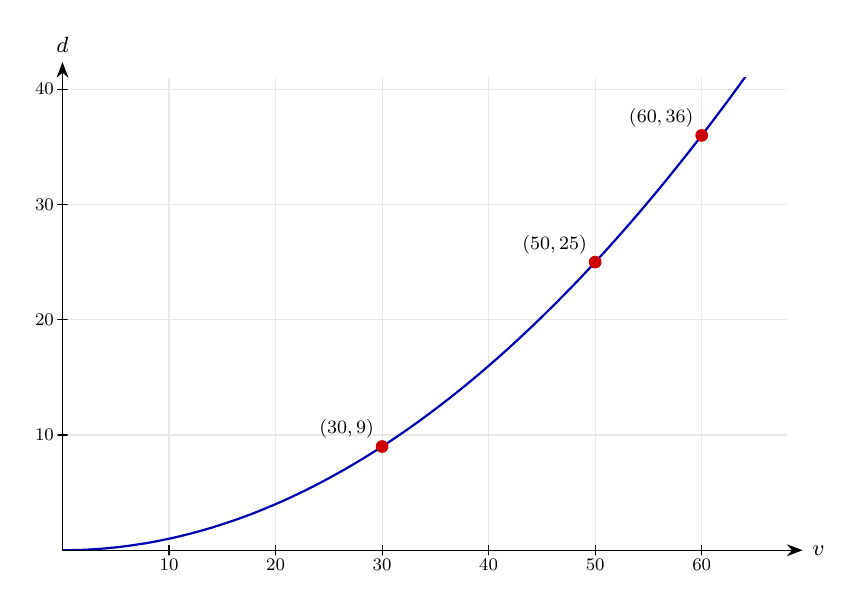
\begin{tikzpicture}[>={Stealth[length=2mm]},font=\footnotesize,line cap=round,line join=round]
\begin{scope}
\clip (0,0) rectangle (9.2,6);
\draw[gray!18] (0,0) grid[xstep=1.353,ystep=1.463] (9.2,6);
\draw[blue!70!black,thick] (0,0) -- (0.046,0) -- (0.092,0.001) -- (0.138,0.002) -- (0.184,0.003) -- (0.23,0.004) -- (0.276,0.006) -- (0.322,0.008) -- (0.368,0.011) -- (0.414,0.014) -- (0.46,0.017) -- (0.506,0.02) -- (0.552,0.024) -- (0.598,0.029) -- (0.644,0.033) -- (0.69,0.038) -- (0.736,0.043) -- (0.782,0.049) -- (0.828,0.055) -- (0.874,0.061) -- (0.92,0.068) -- (0.966,0.075) -- (1.012,0.082) -- (1.058,0.089) -- (1.104,0.097) -- (1.15,0.106) -- (1.196,0.114) -- (1.242,0.123) -- (1.288,0.133) -- (1.334,0.142) -- (1.38,0.152) -- (1.426,0.163) -- (1.472,0.173) -- (1.518,0.184) -- (1.564,0.196) -- (1.61,0.207) -- (1.656,0.219) -- (1.702,0.232) -- (1.748,0.244) -- (1.794,0.257) -- (1.84,0.271) -- (1.886,0.284) -- (1.932,0.298) -- (1.978,0.313) -- (2.024,0.328) -- (2.07,0.343) -- (2.116,0.358) -- (2.162,0.374) -- (2.208,0.39) -- (2.254,0.406) -- (2.3,0.423) -- (2.346,0.44) -- (2.392,0.457) -- (2.438,0.475) -- (2.484,0.493) -- (2.53,0.512) -- (2.576,0.531) -- (2.622,0.55) -- (2.668,0.569) -- (2.714,0.589) -- (2.76,0.609) -- (2.806,0.629) -- (2.852,0.65) -- (2.898,0.671) -- (2.944,0.693) -- (2.99,0.715) -- (3.036,0.737) -- (3.082,0.759) -- (3.128,0.782) -- (3.174,0.805) -- (3.22,0.829) -- (3.266,0.853) -- (3.312,0.877) -- (3.358,0.902) -- (3.404,0.926) -- (3.45,0.952) -- (3.496,0.977) -- (3.542,1.003) -- (3.588,1.029) -- (3.634,1.056) -- (3.68,1.083) -- (3.726,1.11) -- (3.772,1.138) -- (3.818,1.165) -- (3.864,1.194) -- (3.91,1.222) -- (3.956,1.251) -- (4.002,1.28) -- (4.048,1.31) -- (4.094,1.34) -- (4.14,1.37) -- (4.186,1.401) -- (4.232,1.432) -- (4.278,1.463) -- (4.324,1.495) -- (4.37,1.527) -- (4.416,1.559) -- (4.462,1.592) -- (4.508,1.625) -- (4.554,1.658) -- (4.6,1.692) -- (4.646,1.726) -- (4.692,1.76) -- (4.738,1.795) -- (4.784,1.83) -- (4.83,1.865) -- (4.876,1.901) -- (4.922,1.937) -- (4.968,1.973) -- (5.014,2.01) -- (5.06,2.047) -- (5.106,2.084) -- (5.152,2.122) -- (5.198,2.16) -- (5.244,2.199) -- (5.29,2.237) -- (5.336,2.276) -- (5.382,2.316) -- (5.428,2.356) -- (5.474,2.396) -- (5.52,2.436) -- (5.566,2.477) -- (5.612,2.518) -- (5.658,2.559) -- (5.704,2.601) -- (5.75,2.643) -- (5.796,2.686) -- (5.842,2.729) -- (5.888,2.772) -- (5.934,2.815) -- (5.98,2.859) -- (6.026,2.903) -- (6.072,2.948) -- (6.118,2.992) -- (6.164,3.038) -- (6.21,3.083) -- (6.256,3.129) -- (6.302,3.175) -- (6.348,3.222) -- (6.394,3.269) -- (6.44,3.316) -- (6.486,3.363) -- (6.532,3.411) -- (6.578,3.459) -- (6.624,3.508) -- (6.67,3.557) -- (6.716,3.606) -- (6.762,3.656) -- (6.808,3.706) -- (6.854,3.756) -- (6.9,3.806) -- (6.946,3.857) -- (6.992,3.909) -- (7.038,3.96) -- (7.084,4.012) -- (7.13,4.064) -- (7.176,4.117) -- (7.222,4.17) -- (7.268,4.223) -- (7.314,4.277) -- (7.36,4.331) -- (7.406,4.385) -- (7.452,4.44) -- (7.498,4.495) -- (7.544,4.55) -- (7.59,4.606) -- (7.636,4.662) -- (7.682,4.718) -- (7.728,4.775) -- (7.774,4.832) -- (7.82,4.889) -- (7.866,4.947) -- (7.912,5.005) -- (7.958,5.063) -- (8.004,5.122) -- (8.05,5.181) -- (8.096,5.24) -- (8.142,5.3) -- (8.188,5.36) -- (8.234,5.42) -- (8.28,5.481) -- (8.326,5.542) -- (8.372,5.604) -- (8.418,5.665) -- (8.464,5.727) -- (8.51,5.79) -- (8.556,5.853) -- (8.602,5.916) -- (8.648,5.979) -- (8.694,6.043) -- (8.74,6.107) -- (8.786,6.172) -- (8.832,6.236) -- (8.878,6.301) -- (8.924,6.367) -- (8.97,6.433) -- (9.016,6.499) -- (9.062,6.565) -- (9.108,6.632) -- (9.154,6.699) -- (9.2,6.767);
\end{scope}
\draw[->] (0,0) -- (9.4,0) node[right]{$v$};
\draw[->] (0,0) -- (0,6.2) node[above]{$d$};
\draw (1.353,-0.06) -- (1.353,0.06) node[below=2pt,scale=0.8]{$10$};
\draw (2.706,-0.06) -- (2.706,0.06) node[below=2pt,scale=0.8]{$20$};
\draw (4.059,-0.06) -- (4.059,0.06) node[below=2pt,scale=0.8]{$30$};
\draw (5.412,-0.06) -- (5.412,0.06) node[below=2pt,scale=0.8]{$40$};
\draw (6.765,-0.06) -- (6.765,0.06) node[below=2pt,scale=0.8]{$50$};
\draw (8.118,-0.06) -- (8.118,0.06) node[below=2pt,scale=0.8]{$60$};
\draw (-0.06,1.463) -- (0.06,1.463) node[left=2pt,scale=0.8]{$10$};
\draw (-0.06,2.927) -- (0.06,2.927) node[left=2pt,scale=0.8]{$20$};
\draw (-0.06,4.39) -- (0.06,4.39) node[left=2pt,scale=0.8]{$30$};
\draw (-0.06,5.854) -- (0.06,5.854) node[left=2pt,scale=0.8]{$40$};
\fill[red!80!black] (4.059,1.317) circle (2.3pt);
\node[above left,scale=0.85] at (4.059,1.317) {$(30,9)$};
\fill[red!80!black] (6.765,3.659) circle (2.3pt);
\node[above left,scale=0.85] at (6.765,3.659) {$(50,25)$};
\fill[red!80!black] (8.118,5.268) circle (2.3pt);
\node[above left,scale=0.85] at (8.118,5.268) {$(60,36)$};
\end{tikzpicture}
}
\end{center}
\small The relationship plotted, with the data points marked.\normalsize

\medskip\hrule

\section*{Proportion 20\quad\small\texttt{(cg4-020)}}
\addcontentsline{toc}{section}{Proportion 20 (cg4-020)}
\textit{Difficulty: Foundation \quad\textbar\quad Marks: 4}

\question{Given that \( y \propto x^2 \) and \( y = 12 \) when \( x = 2 \), sketch the graph of \( y \) against \( x \) for \( x \geq 0 \) and find \( y \) when \( x = 3 \).}

\textbf{Worked solution.}

\textit{Step 1: Find \( k \).}
\[\begin{gathered}
12 = k \times 4 \implies k = 3
\end{gathered}\]
Substitute the known values.

\textit{Step 2: State the equation.}
\[\begin{gathered}
y = 3x^2
\end{gathered}\]
This is a parabola through the origin.

\textit{Step 3: Describe the sketch.}
\[\begin{gathered}
\text{Graph: parabola through } (0,0),\ (1,3),\ (2,12),\ (3,27)
\end{gathered}\]
The curve starts at the origin, opens upward, passes through the points listed.

\textit{Step 4: Find \( y \) when \( x = 3 \).}
\[\begin{gathered}
y = 3 \times 9 = 27
\end{gathered}\]
Square \( x \) then multiply by \( k \).

\begin{answerbox}
\textbf{Final answer:}\quad \(\displaystyle  y = 27 \) when \(\displaystyle  x = 3 \); graph is a parabola through the origin.
\end{answerbox}
\textbf{Graph.}

\begin{center}
\resizebox{\ifdim\width>\linewidth \linewidth\else \width\fi}{!}{%
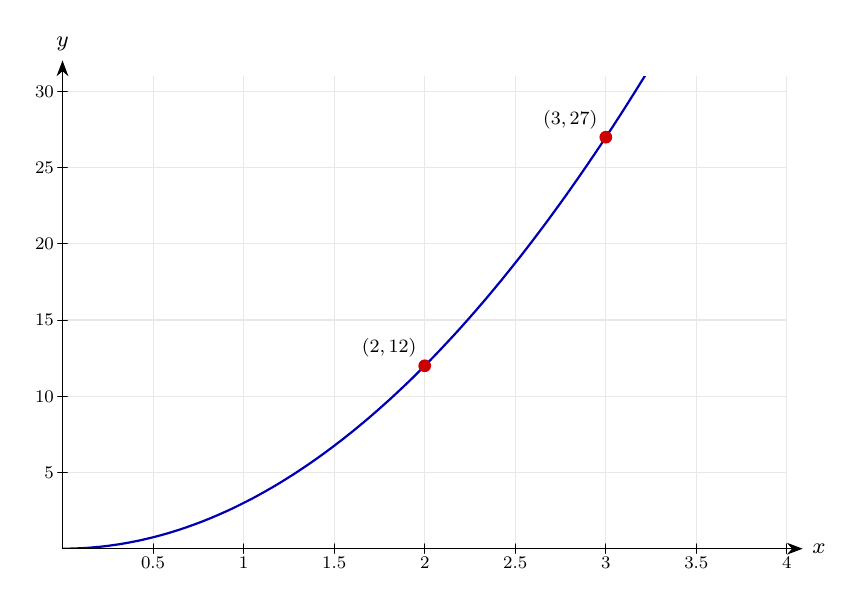
\begin{tikzpicture}[>={Stealth[length=2mm]},font=\footnotesize,line cap=round,line join=round]
\begin{scope}
\clip (0,0) rectangle (9.2,6);
\draw[gray!18] (0,0) grid[xstep=1.15,ystep=0.968] (9.2,6);
\draw[blue!70!black,thick] (0,0) -- (0.046,0) -- (0.092,0.001) -- (0.138,0.002) -- (0.184,0.004) -- (0.23,0.006) -- (0.276,0.008) -- (0.322,0.011) -- (0.368,0.015) -- (0.414,0.019) -- (0.46,0.023) -- (0.506,0.028) -- (0.552,0.033) -- (0.598,0.039) -- (0.644,0.046) -- (0.69,0.052) -- (0.736,0.059) -- (0.782,0.067) -- (0.828,0.075) -- (0.874,0.084) -- (0.92,0.093) -- (0.966,0.102) -- (1.012,0.112) -- (1.058,0.123) -- (1.104,0.134) -- (1.15,0.145) -- (1.196,0.157) -- (1.242,0.169) -- (1.288,0.182) -- (1.334,0.195) -- (1.38,0.209) -- (1.426,0.223) -- (1.472,0.238) -- (1.518,0.253) -- (1.564,0.268) -- (1.61,0.285) -- (1.656,0.301) -- (1.702,0.318) -- (1.748,0.335) -- (1.794,0.353) -- (1.84,0.372) -- (1.886,0.39) -- (1.932,0.41) -- (1.978,0.429) -- (2.024,0.45) -- (2.07,0.47) -- (2.116,0.491) -- (2.162,0.513) -- (2.208,0.535) -- (2.254,0.558) -- (2.3,0.581) -- (2.346,0.604) -- (2.392,0.628) -- (2.438,0.652) -- (2.484,0.677) -- (2.53,0.703) -- (2.576,0.728) -- (2.622,0.755) -- (2.668,0.781) -- (2.714,0.808) -- (2.76,0.836) -- (2.806,0.864) -- (2.852,0.893) -- (2.898,0.922) -- (2.944,0.951) -- (2.99,0.981) -- (3.036,1.012) -- (3.082,1.043) -- (3.128,1.074) -- (3.174,1.106) -- (3.22,1.138) -- (3.266,1.171) -- (3.312,1.204) -- (3.358,1.238) -- (3.404,1.272) -- (3.45,1.306) -- (3.496,1.342) -- (3.542,1.377) -- (3.588,1.413) -- (3.634,1.45) -- (3.68,1.486) -- (3.726,1.524) -- (3.772,1.562) -- (3.818,1.6) -- (3.864,1.639) -- (3.91,1.678) -- (3.956,1.718) -- (4.002,1.758) -- (4.048,1.799) -- (4.094,1.84) -- (4.14,1.881) -- (4.186,1.923) -- (4.232,1.966) -- (4.278,2.009) -- (4.324,2.052) -- (4.37,2.096) -- (4.416,2.14) -- (4.462,2.185) -- (4.508,2.231) -- (4.554,2.276) -- (4.6,2.323) -- (4.646,2.369) -- (4.692,2.416) -- (4.738,2.464) -- (4.784,2.512) -- (4.83,2.561) -- (4.876,2.61) -- (4.922,2.659) -- (4.968,2.709) -- (5.014,2.759) -- (5.06,2.81) -- (5.106,2.862) -- (5.152,2.913) -- (5.198,2.966) -- (5.244,3.018) -- (5.29,3.072) -- (5.336,3.125) -- (5.382,3.179) -- (5.428,3.234) -- (5.474,3.289) -- (5.52,3.345) -- (5.566,3.4) -- (5.612,3.457) -- (5.658,3.514) -- (5.704,3.571) -- (5.75,3.629) -- (5.796,3.687) -- (5.842,3.746) -- (5.888,3.805) -- (5.934,3.865) -- (5.98,3.925) -- (6.026,3.986) -- (6.072,4.047) -- (6.118,4.108) -- (6.164,4.17) -- (6.21,4.233) -- (6.256,4.296) -- (6.302,4.359) -- (6.348,4.423) -- (6.394,4.487) -- (6.44,4.552) -- (6.486,4.618) -- (6.532,4.683) -- (6.578,4.749) -- (6.624,4.816) -- (6.67,4.883) -- (6.716,4.951) -- (6.762,5.019) -- (6.808,5.087) -- (6.854,5.156) -- (6.9,5.226) -- (6.946,5.296) -- (6.992,5.366) -- (7.038,5.437) -- (7.084,5.508) -- (7.13,5.58) -- (7.176,5.652) -- (7.222,5.725) -- (7.268,5.798) -- (7.314,5.872) -- (7.36,5.946) -- (7.406,6.02) -- (7.452,6.095) -- (7.498,6.171) -- (7.544,6.247) -- (7.59,6.323) -- (7.636,6.4) -- (7.682,6.477) -- (7.728,6.555) -- (7.774,6.634) -- (7.82,6.712) -- (7.866,6.791) -- (7.912,6.871) -- (7.958,6.951) -- (8.004,7.032) -- (8.05,7.113) -- (8.096,7.194) -- (8.142,7.276) -- (8.188,7.359) -- (8.234,7.442) -- (8.28,7.525) -- (8.326,7.609) -- (8.372,7.693) -- (8.418,7.778) -- (8.464,7.863) -- (8.51,7.949) -- (8.556,8.035) -- (8.602,8.122) -- (8.648,8.209) -- (8.694,8.296) -- (8.74,8.385) -- (8.786,8.473) -- (8.832,8.562) -- (8.878,8.651) -- (8.924,8.741) -- (8.97,8.832) -- (9.016,8.922) -- (9.062,9.014) -- (9.108,9.105) -- (9.154,9.198) -- (9.2,9.29);
\end{scope}
\draw[->] (0,0) -- (9.4,0) node[right]{$x$};
\draw[->] (0,0) -- (0,6.2) node[above]{$y$};
\draw (1.15,-0.06) -- (1.15,0.06) node[below=2pt,scale=0.8]{$0.5$};
\draw (2.3,-0.06) -- (2.3,0.06) node[below=2pt,scale=0.8]{$1$};
\draw (3.45,-0.06) -- (3.45,0.06) node[below=2pt,scale=0.8]{$1.5$};
\draw (4.6,-0.06) -- (4.6,0.06) node[below=2pt,scale=0.8]{$2$};
\draw (5.75,-0.06) -- (5.75,0.06) node[below=2pt,scale=0.8]{$2.5$};
\draw (6.9,-0.06) -- (6.9,0.06) node[below=2pt,scale=0.8]{$3$};
\draw (8.05,-0.06) -- (8.05,0.06) node[below=2pt,scale=0.8]{$3.5$};
\draw (9.2,-0.06) -- (9.2,0.06) node[below=2pt,scale=0.8]{$4$};
\draw (-0.06,0.968) -- (0.06,0.968) node[left=2pt,scale=0.8]{$5$};
\draw (-0.06,1.935) -- (0.06,1.935) node[left=2pt,scale=0.8]{$10$};
\draw (-0.06,2.903) -- (0.06,2.903) node[left=2pt,scale=0.8]{$15$};
\draw (-0.06,3.871) -- (0.06,3.871) node[left=2pt,scale=0.8]{$20$};
\draw (-0.06,4.839) -- (0.06,4.839) node[left=2pt,scale=0.8]{$25$};
\draw (-0.06,5.806) -- (0.06,5.806) node[left=2pt,scale=0.8]{$30$};
\fill[red!80!black] (4.6,2.323) circle (2.3pt);
\node[above left,scale=0.85] at (4.6,2.323) {$(2,12)$};
\fill[red!80!black] (6.9,5.226) circle (2.3pt);
\node[above left,scale=0.85] at (6.9,5.226) {$(3,27)$};
\end{tikzpicture}
}
\end{center}
\small The relationship plotted, with the data points marked.\normalsize

\medskip\hrule

\section*{Proportion 21\quad\small\texttt{(cg4-021)}}
\addcontentsline{toc}{section}{Proportion 21 (cg4-021)}
\textit{Difficulty: Foundation \quad\textbar\quad Marks: 3}

\question{The power \( P \) watts dissipated in a resistor is directly proportional to the square of the current \( I \) amps. When \( I = 3 \) A, \( P = 45 \) W. Find \( P \) when \( I = 5 \) A.}

\textbf{Worked solution.}

\textit{Step 1: Write \( P = kI^2 \) and find \( k \).}
\[\begin{gathered}
45 = k \times 9 \implies k = 5
\end{gathered}\]
\( 3^2 = 9 \); divide both sides by 9.

\textit{Step 2: Substitute \( I = 5 \).}
\[\begin{gathered}
P = 5 \times 25 = 125 \text{ W}
\end{gathered}\]
The power dissipated is 125 W.

\begin{answerbox}
\textbf{Final answer:}\quad \(\displaystyle  P = 125 \) W
\end{answerbox}
\textbf{Graph.}

\begin{center}
\resizebox{\ifdim\width>\linewidth \linewidth\else \width\fi}{!}{%
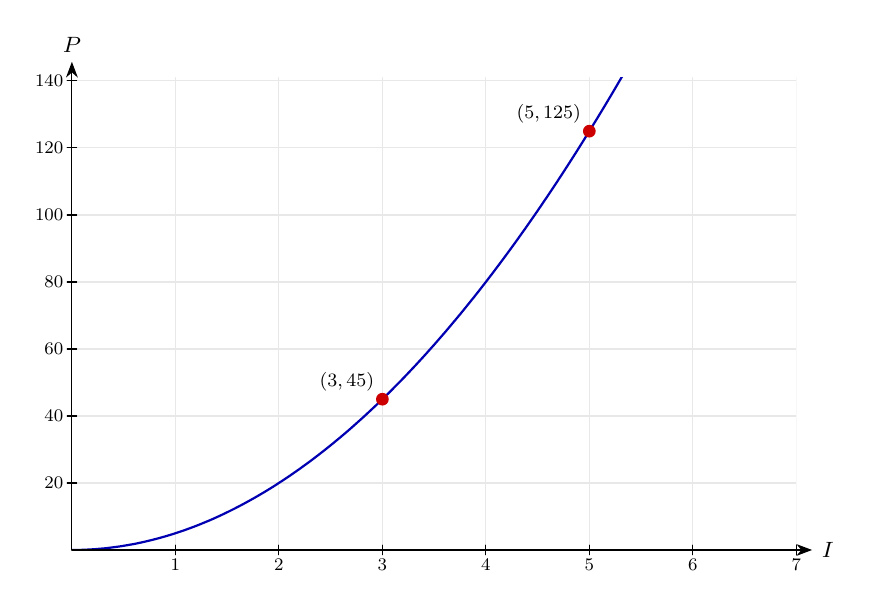
\begin{tikzpicture}[>={Stealth[length=2mm]},font=\footnotesize,line cap=round,line join=round]
\begin{scope}
\clip (0,0) rectangle (9.2,6);
\draw[gray!18] (0,0) grid[xstep=1.314,ystep=0.851] (9.2,6);
\draw[blue!70!black,thick] (0,0) -- (0.046,0) -- (0.092,0.001) -- (0.138,0.002) -- (0.184,0.004) -- (0.23,0.007) -- (0.276,0.009) -- (0.322,0.013) -- (0.368,0.017) -- (0.414,0.021) -- (0.46,0.026) -- (0.506,0.032) -- (0.552,0.038) -- (0.598,0.044) -- (0.644,0.051) -- (0.69,0.059) -- (0.736,0.067) -- (0.782,0.075) -- (0.828,0.084) -- (0.874,0.094) -- (0.92,0.104) -- (0.966,0.115) -- (1.012,0.126) -- (1.058,0.138) -- (1.104,0.15) -- (1.15,0.163) -- (1.196,0.176) -- (1.242,0.19) -- (1.288,0.204) -- (1.334,0.219) -- (1.38,0.235) -- (1.426,0.25) -- (1.472,0.267) -- (1.518,0.284) -- (1.564,0.301) -- (1.61,0.319) -- (1.656,0.338) -- (1.702,0.357) -- (1.748,0.376) -- (1.794,0.396) -- (1.84,0.417) -- (1.886,0.438) -- (1.932,0.46) -- (1.978,0.482) -- (2.024,0.505) -- (2.07,0.528) -- (2.116,0.552) -- (2.162,0.576) -- (2.208,0.601) -- (2.254,0.626) -- (2.3,0.652) -- (2.346,0.678) -- (2.392,0.705) -- (2.438,0.732) -- (2.484,0.76) -- (2.53,0.788) -- (2.576,0.817) -- (2.622,0.847) -- (2.668,0.877) -- (2.714,0.907) -- (2.76,0.938) -- (2.806,0.97) -- (2.852,1.002) -- (2.898,1.034) -- (2.944,1.068) -- (2.99,1.101) -- (3.036,1.135) -- (3.082,1.17) -- (3.128,1.205) -- (3.174,1.241) -- (3.22,1.277) -- (3.266,1.314) -- (3.312,1.351) -- (3.358,1.389) -- (3.404,1.427) -- (3.45,1.466) -- (3.496,1.505) -- (3.542,1.545) -- (3.588,1.586) -- (3.634,1.627) -- (3.68,1.668) -- (3.726,1.71) -- (3.772,1.753) -- (3.818,1.796) -- (3.864,1.839) -- (3.91,1.883) -- (3.956,1.928) -- (4.002,1.973) -- (4.048,2.018) -- (4.094,2.065) -- (4.14,2.111) -- (4.186,2.158) -- (4.232,2.206) -- (4.278,2.254) -- (4.324,2.303) -- (4.37,2.352) -- (4.416,2.402) -- (4.462,2.452) -- (4.508,2.503) -- (4.554,2.555) -- (4.6,2.606) -- (4.646,2.659) -- (4.692,2.712) -- (4.738,2.765) -- (4.784,2.819) -- (4.83,2.874) -- (4.876,2.929) -- (4.922,2.984) -- (4.968,3.04) -- (5.014,3.097) -- (5.06,3.154) -- (5.106,3.211) -- (5.152,3.269) -- (5.198,3.328) -- (5.244,3.387) -- (5.29,3.447) -- (5.336,3.507) -- (5.382,3.568) -- (5.428,3.629) -- (5.474,3.691) -- (5.52,3.753) -- (5.566,3.816) -- (5.612,3.879) -- (5.658,3.943) -- (5.704,4.008) -- (5.75,4.072) -- (5.796,4.138) -- (5.842,4.204) -- (5.888,4.27) -- (5.934,4.337) -- (5.98,4.405) -- (6.026,4.473) -- (6.072,4.541) -- (6.118,4.61) -- (6.164,4.68) -- (6.21,4.75) -- (6.256,4.821) -- (6.302,4.892) -- (6.348,4.964) -- (6.394,5.036) -- (6.44,5.109) -- (6.486,5.182) -- (6.532,5.256) -- (6.578,5.33) -- (6.624,5.405) -- (6.67,5.48) -- (6.716,5.556) -- (6.762,5.632) -- (6.808,5.709) -- (6.854,5.786) -- (6.9,5.864) -- (6.946,5.943) -- (6.992,6.022) -- (7.038,6.101) -- (7.084,6.181) -- (7.13,6.262) -- (7.176,6.343) -- (7.222,6.424) -- (7.268,6.507) -- (7.314,6.589) -- (7.36,6.672) -- (7.406,6.756) -- (7.452,6.84) -- (7.498,6.925) -- (7.544,7.01) -- (7.59,7.096) -- (7.636,7.182) -- (7.682,7.269) -- (7.728,7.356) -- (7.774,7.444) -- (7.82,7.532) -- (7.866,7.621) -- (7.912,7.711) -- (7.958,7.801) -- (8.004,7.891) -- (8.05,7.982) -- (8.096,8.074) -- (8.142,8.166) -- (8.188,8.258) -- (8.234,8.351) -- (8.28,8.445) -- (8.326,8.539) -- (8.372,8.633) -- (8.418,8.729) -- (8.464,8.824) -- (8.51,8.92) -- (8.556,9.017) -- (8.602,9.114) -- (8.648,9.212) -- (8.694,9.31) -- (8.74,9.409) -- (8.786,9.508) -- (8.832,9.608) -- (8.878,9.709) -- (8.924,9.809) -- (8.97,9.911) -- (9.016,10.013) -- (9.062,10.115) -- (9.108,10.218) -- (9.154,10.322) -- (9.2,10.426);
\end{scope}
\draw[->] (0,0) -- (9.4,0) node[right]{$I$};
\draw[->] (0,0) -- (0,6.2) node[above]{$P$};
\draw (1.314,-0.06) -- (1.314,0.06) node[below=2pt,scale=0.8]{$1$};
\draw (2.629,-0.06) -- (2.629,0.06) node[below=2pt,scale=0.8]{$2$};
\draw (3.943,-0.06) -- (3.943,0.06) node[below=2pt,scale=0.8]{$3$};
\draw (5.257,-0.06) -- (5.257,0.06) node[below=2pt,scale=0.8]{$4$};
\draw (6.571,-0.06) -- (6.571,0.06) node[below=2pt,scale=0.8]{$5$};
\draw (7.886,-0.06) -- (7.886,0.06) node[below=2pt,scale=0.8]{$6$};
\draw (9.2,-0.06) -- (9.2,0.06) node[below=2pt,scale=0.8]{$7$};
\draw (-0.06,0.851) -- (0.06,0.851) node[left=2pt,scale=0.8]{$20$};
\draw (-0.06,1.702) -- (0.06,1.702) node[left=2pt,scale=0.8]{$40$};
\draw (-0.06,2.553) -- (0.06,2.553) node[left=2pt,scale=0.8]{$60$};
\draw (-0.06,3.404) -- (0.06,3.404) node[left=2pt,scale=0.8]{$80$};
\draw (-0.06,4.255) -- (0.06,4.255) node[left=2pt,scale=0.8]{$100$};
\draw (-0.06,5.106) -- (0.06,5.106) node[left=2pt,scale=0.8]{$120$};
\draw (-0.06,5.957) -- (0.06,5.957) node[left=2pt,scale=0.8]{$140$};
\fill[red!80!black] (3.943,1.915) circle (2.3pt);
\node[above left,scale=0.85] at (3.943,1.915) {$(3,45)$};
\fill[red!80!black] (6.571,5.319) circle (2.3pt);
\node[above left,scale=0.85] at (6.571,5.319) {$(5,125)$};
\end{tikzpicture}
}
\end{center}
\small The relationship plotted, with the data points marked.\normalsize

\medskip\hrule

\section*{Proportion 22\quad\small\texttt{(cg4-022)}}
\addcontentsline{toc}{section}{Proportion 22 (cg4-022)}
\textit{Difficulty: Foundation \quad\textbar\quad Marks: 3}

\question{Given that \( y \propto \dfrac{1}{x^2} \) and that \( y = 16 \) when \( x = 3 \), find \( y \) when \( x = 6 \).}

\textbf{Worked solution.}

\textit{Step 1: Write \( y = \frac{k}{x^2} \) and find \( k \).}
\[\begin{gathered}
16 = \frac{k}{9} \implies k = 144
\end{gathered}\]
Multiply both sides by \( 3^2 = 9 \).

\textit{Step 2: Substitute \( x = 6 \).}
\[\begin{gathered}
y = \frac{144}{36} = 4
\end{gathered}\]
When \( x \) doubles, \( y \) decreases by a factor of 4.

\begin{answerbox}
\textbf{Final answer:}\quad \(\displaystyle  y = 4 \)
\end{answerbox}
\textbf{Graph.}

\begin{center}
\resizebox{\ifdim\width>\linewidth \linewidth\else \width\fi}{!}{%
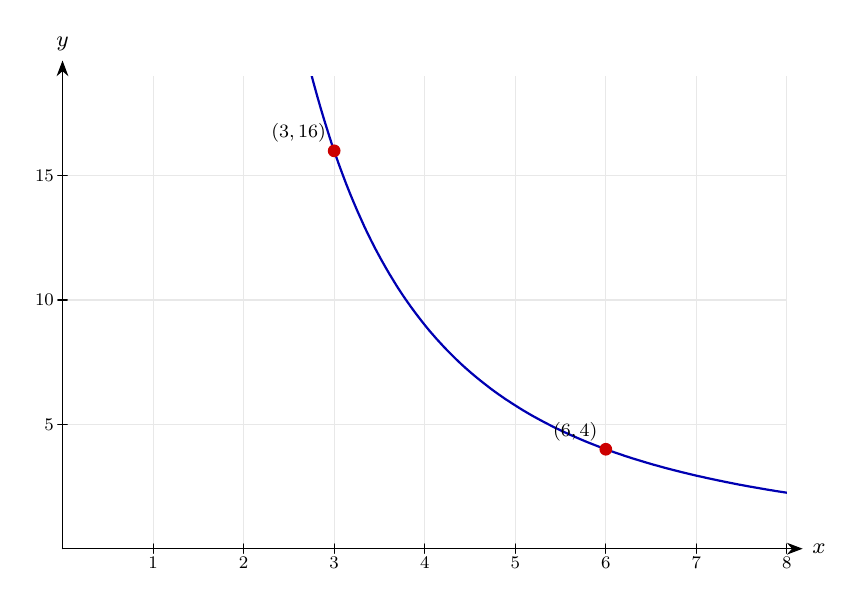
\begin{tikzpicture}[>={Stealth[length=2mm]},font=\footnotesize,line cap=round,line join=round]
\begin{scope}
\clip (0,0) rectangle (9.2,6);
\draw[gray!18] (0,0) grid[xstep=1.15,ystep=1.579] (9.2,6);
\draw[blue!70!black,thick] (0.023,12) -- (0.069,12) -- (0.115,12) -- (0.161,12) -- (0.207,12) -- (0.252,12) -- (0.298,12) -- (0.344,12) -- (0.39,12) -- (0.436,12) -- (0.482,12) -- (0.528,12) -- (0.574,12) -- (0.62,12) -- (0.665,12) -- (0.711,12) -- (0.757,12) -- (0.803,12) -- (0.849,12) -- (0.895,12) -- (0.941,12) -- (0.987,12) -- (1.032,12) -- (1.078,12) -- (1.124,12) -- (1.17,12) -- (1.216,12) -- (1.262,12) -- (1.308,12) -- (1.354,12) -- (1.4,12) -- (1.445,12) -- (1.491,12) -- (1.537,12) -- (1.583,12) -- (1.629,12) -- (1.675,12) -- (1.721,12) -- (1.767,12) -- (1.813,12) -- (1.858,12) -- (1.904,12) -- (1.95,12) -- (1.996,12) -- (2.042,12) -- (2.088,12) -- (2.134,12) -- (2.18,12) -- (2.225,12) -- (2.271,11.657) -- (2.317,11.2) -- (2.363,10.769) -- (2.409,10.363) -- (2.455,9.979) -- (2.501,9.616) -- (2.547,9.273) -- (2.593,8.947) -- (2.638,8.639) -- (2.684,8.346) -- (2.73,8.068) -- (2.776,7.803) -- (2.822,7.552) -- (2.868,7.312) -- (2.914,7.084) -- (2.96,6.866) -- (3.006,6.658) -- (3.051,6.459) -- (3.097,6.269) -- (3.143,6.087) -- (3.189,5.913) -- (3.235,5.747) -- (3.281,5.587) -- (3.327,5.434) -- (3.373,5.287) -- (3.418,5.146) -- (3.464,5.011) -- (3.51,4.881) -- (3.556,4.756) -- (3.602,4.635) -- (3.648,4.519) -- (3.694,4.408) -- (3.74,4.3) -- (3.786,4.197) -- (3.831,4.097) -- (3.877,4) -- (3.923,3.907) -- (3.969,3.817) -- (4.015,3.731) -- (4.061,3.647) -- (4.107,3.566) -- (4.153,3.487) -- (4.199,3.412) -- (4.244,3.338) -- (4.29,3.267) -- (4.336,3.198) -- (4.382,3.132) -- (4.428,3.067) -- (4.474,3.005) -- (4.52,2.944) -- (4.566,2.885) -- (4.611,2.828) -- (4.657,2.772) -- (4.703,2.719) -- (4.749,2.666) -- (4.795,2.616) -- (4.841,2.566) -- (4.887,2.518) -- (4.933,2.472) -- (4.979,2.426) -- (5.024,2.382) -- (5.07,2.339) -- (5.116,2.297) -- (5.162,2.257) -- (5.208,2.217) -- (5.254,2.179) -- (5.3,2.141) -- (5.346,2.105) -- (5.392,2.069) -- (5.437,2.034) -- (5.483,2) -- (5.529,1.967) -- (5.575,1.935) -- (5.621,1.903) -- (5.667,1.873) -- (5.713,1.843) -- (5.759,1.814) -- (5.805,1.785) -- (5.85,1.757) -- (5.896,1.73) -- (5.942,1.703) -- (5.988,1.677) -- (6.034,1.652) -- (6.08,1.627) -- (6.126,1.603) -- (6.172,1.579) -- (6.217,1.556) -- (6.263,1.533) -- (6.309,1.511) -- (6.355,1.489) -- (6.401,1.468) -- (6.447,1.447) -- (6.493,1.427) -- (6.539,1.407) -- (6.585,1.387) -- (6.63,1.368) -- (6.676,1.349) -- (6.722,1.331) -- (6.768,1.313) -- (6.814,1.295) -- (6.86,1.278) -- (6.906,1.261) -- (6.952,1.244) -- (6.998,1.228) -- (7.043,1.212) -- (7.089,1.197) -- (7.135,1.181) -- (7.181,1.166) -- (7.227,1.151) -- (7.273,1.137) -- (7.319,1.123) -- (7.365,1.109) -- (7.41,1.095) -- (7.456,1.082) -- (7.502,1.068) -- (7.548,1.056) -- (7.594,1.043) -- (7.64,1.03) -- (7.686,1.018) -- (7.732,1.006) -- (7.778,0.994) -- (7.823,0.983) -- (7.869,0.971) -- (7.915,0.96) -- (7.961,0.949) -- (8.007,0.938) -- (8.053,0.927) -- (8.099,0.917) -- (8.145,0.907) -- (8.191,0.896) -- (8.236,0.887) -- (8.282,0.877) -- (8.328,0.867) -- (8.374,0.858) -- (8.42,0.848) -- (8.466,0.839) -- (8.512,0.83) -- (8.558,0.821) -- (8.603,0.812) -- (8.649,0.804) -- (8.695,0.795) -- (8.741,0.787) -- (8.787,0.779) -- (8.833,0.771) -- (8.879,0.763) -- (8.925,0.755) -- (8.971,0.747) -- (9.016,0.74) -- (9.062,0.732) -- (9.108,0.725) -- (9.154,0.718) -- (9.2,0.711);
\end{scope}
\draw[->] (0,0) -- (9.4,0) node[right]{$x$};
\draw[->] (0,0) -- (0,6.2) node[above]{$y$};
\draw (1.15,-0.06) -- (1.15,0.06) node[below=2pt,scale=0.8]{$1$};
\draw (2.3,-0.06) -- (2.3,0.06) node[below=2pt,scale=0.8]{$2$};
\draw (3.45,-0.06) -- (3.45,0.06) node[below=2pt,scale=0.8]{$3$};
\draw (4.6,-0.06) -- (4.6,0.06) node[below=2pt,scale=0.8]{$4$};
\draw (5.75,-0.06) -- (5.75,0.06) node[below=2pt,scale=0.8]{$5$};
\draw (6.9,-0.06) -- (6.9,0.06) node[below=2pt,scale=0.8]{$6$};
\draw (8.05,-0.06) -- (8.05,0.06) node[below=2pt,scale=0.8]{$7$};
\draw (9.2,-0.06) -- (9.2,0.06) node[below=2pt,scale=0.8]{$8$};
\draw (-0.06,1.579) -- (0.06,1.579) node[left=2pt,scale=0.8]{$5$};
\draw (-0.06,3.158) -- (0.06,3.158) node[left=2pt,scale=0.8]{$10$};
\draw (-0.06,4.737) -- (0.06,4.737) node[left=2pt,scale=0.8]{$15$};
\fill[red!80!black] (3.45,5.053) circle (2.3pt);
\node[above left,scale=0.85] at (3.45,5.053) {$(3,16)$};
\fill[red!80!black] (6.9,1.263) circle (2.3pt);
\node[above left,scale=0.85] at (6.9,1.263) {$(6,4)$};
\end{tikzpicture}
}
\end{center}
\small The relationship plotted, with the data points marked.\normalsize

\medskip\hrule

\section*{Proportion 23\quad\small\texttt{(cg4-023)}}
\addcontentsline{toc}{section}{Proportion 23 (cg4-023)}
\textit{Difficulty: Foundation \quad\textbar\quad Marks: 3}

\question{The intensity \( I \) of light from a lamp is inversely proportional to the square of the distance \( d \) metres from the lamp. At \( d = 2 \) m, \( I = 50 \) lux. Find \( I \) when \( d = 5 \) m.}

\textbf{Worked solution.}

\textit{Step 1: Write \( I = \frac{k}{d^2} \) and find \( k \).}
\[\begin{gathered}
50 = \frac{k}{4} \implies k = 200
\end{gathered}\]
Multiply both sides by \( 2^2 = 4 \).

\textit{Step 2: Substitute \( d = 5 \).}
\[\begin{gathered}
I = \frac{200}{25} = 8 \text{ lux}
\end{gathered}\]
The intensity decreases sharply as distance increases.

\begin{answerbox}
\textbf{Final answer:}\quad \(\displaystyle  I = 8 \) lux
\end{answerbox}
\textbf{Graph.}

\begin{center}
\resizebox{\ifdim\width>\linewidth \linewidth\else \width\fi}{!}{%
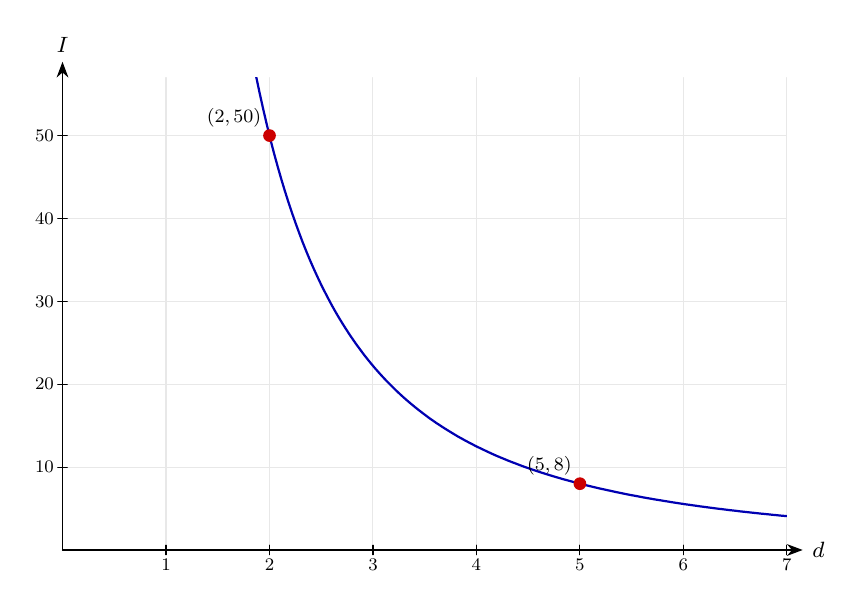
\begin{tikzpicture}[>={Stealth[length=2mm]},font=\footnotesize,line cap=round,line join=round]
\begin{scope}
\clip (0,0) rectangle (9.2,6);
\draw[gray!18] (0,0) grid[xstep=1.314,ystep=1.053] (9.2,6);
\draw[blue!70!black,thick] (0.023,12) -- (0.069,12) -- (0.115,12) -- (0.161,12) -- (0.207,12) -- (0.252,12) -- (0.298,12) -- (0.344,12) -- (0.39,12) -- (0.436,12) -- (0.482,12) -- (0.528,12) -- (0.574,12) -- (0.62,12) -- (0.665,12) -- (0.711,12) -- (0.757,12) -- (0.803,12) -- (0.849,12) -- (0.895,12) -- (0.941,12) -- (0.987,12) -- (1.032,12) -- (1.078,12) -- (1.124,12) -- (1.17,12) -- (1.216,12) -- (1.262,12) -- (1.308,12) -- (1.354,12) -- (1.4,12) -- (1.445,12) -- (1.491,12) -- (1.537,12) -- (1.583,12) -- (1.629,12) -- (1.675,12) -- (1.721,12) -- (1.767,11.652) -- (1.813,11.069) -- (1.858,10.529) -- (1.904,10.028) -- (1.95,9.562) -- (1.996,9.127) -- (2.042,8.722) -- (2.088,8.343) -- (2.134,7.988) -- (2.18,7.655) -- (2.225,7.342) -- (2.271,7.049) -- (2.317,6.772) -- (2.363,6.512) -- (2.409,6.266) -- (2.455,6.034) -- (2.501,5.815) -- (2.547,5.607) -- (2.593,5.41) -- (2.638,5.224) -- (2.684,5.047) -- (2.73,4.879) -- (2.776,4.719) -- (2.822,4.566) -- (2.868,4.421) -- (2.914,4.283) -- (2.96,4.152) -- (3.006,4.026) -- (3.051,3.906) -- (3.097,3.791) -- (3.143,3.681) -- (3.189,3.576) -- (3.235,3.475) -- (3.281,3.378) -- (3.327,3.286) -- (3.373,3.197) -- (3.418,3.112) -- (3.464,3.03) -- (3.51,2.951) -- (3.556,2.876) -- (3.602,2.803) -- (3.648,2.733) -- (3.694,2.665) -- (3.74,2.6) -- (3.786,2.538) -- (3.831,2.477) -- (3.877,2.419) -- (3.923,2.363) -- (3.969,2.308) -- (4.015,2.256) -- (4.061,2.205) -- (4.107,2.156) -- (4.153,2.109) -- (4.199,2.063) -- (4.244,2.019) -- (4.29,1.976) -- (4.336,1.934) -- (4.382,1.894) -- (4.428,1.855) -- (4.474,1.817) -- (4.52,1.78) -- (4.566,1.745) -- (4.612,1.71) -- (4.657,1.676) -- (4.703,1.644) -- (4.749,1.612) -- (4.795,1.582) -- (4.841,1.552) -- (4.887,1.523) -- (4.933,1.495) -- (4.979,1.467) -- (5.024,1.44) -- (5.07,1.415) -- (5.116,1.389) -- (5.162,1.365) -- (5.208,1.341) -- (5.254,1.317) -- (5.3,1.295) -- (5.346,1.273) -- (5.392,1.251) -- (5.437,1.23) -- (5.483,1.209) -- (5.529,1.189) -- (5.575,1.17) -- (5.621,1.151) -- (5.667,1.132) -- (5.713,1.114) -- (5.759,1.097) -- (5.805,1.079) -- (5.85,1.062) -- (5.896,1.046) -- (5.942,1.03) -- (5.988,1.014) -- (6.034,0.999) -- (6.08,0.984) -- (6.126,0.969) -- (6.172,0.955) -- (6.217,0.941) -- (6.263,0.927) -- (6.309,0.914) -- (6.355,0.9) -- (6.401,0.888) -- (6.447,0.875) -- (6.493,0.863) -- (6.539,0.851) -- (6.585,0.839) -- (6.63,0.827) -- (6.676,0.816) -- (6.722,0.805) -- (6.768,0.794) -- (6.814,0.783) -- (6.86,0.773) -- (6.906,0.763) -- (6.952,0.753) -- (6.998,0.743) -- (7.043,0.733) -- (7.089,0.724) -- (7.135,0.714) -- (7.181,0.705) -- (7.227,0.696) -- (7.273,0.688) -- (7.319,0.679) -- (7.365,0.67) -- (7.41,0.662) -- (7.456,0.654) -- (7.502,0.646) -- (7.548,0.638) -- (7.594,0.631) -- (7.64,0.623) -- (7.686,0.616) -- (7.732,0.608) -- (7.778,0.601) -- (7.823,0.594) -- (7.869,0.587) -- (7.915,0.58) -- (7.961,0.574) -- (8.007,0.567) -- (8.053,0.561) -- (8.099,0.554) -- (8.145,0.548) -- (8.191,0.542) -- (8.236,0.536) -- (8.282,0.53) -- (8.328,0.524) -- (8.374,0.519) -- (8.42,0.513) -- (8.466,0.507) -- (8.512,0.502) -- (8.558,0.497) -- (8.603,0.491) -- (8.649,0.486) -- (8.695,0.481) -- (8.741,0.476) -- (8.787,0.471) -- (8.833,0.466) -- (8.879,0.461) -- (8.925,0.457) -- (8.971,0.452) -- (9.016,0.447) -- (9.062,0.443) -- (9.108,0.438) -- (9.154,0.434) -- (9.2,0.43);
\end{scope}
\draw[->] (0,0) -- (9.4,0) node[right]{$d$};
\draw[->] (0,0) -- (0,6.2) node[above]{$I$};
\draw (1.314,-0.06) -- (1.314,0.06) node[below=2pt,scale=0.8]{$1$};
\draw (2.629,-0.06) -- (2.629,0.06) node[below=2pt,scale=0.8]{$2$};
\draw (3.943,-0.06) -- (3.943,0.06) node[below=2pt,scale=0.8]{$3$};
\draw (5.257,-0.06) -- (5.257,0.06) node[below=2pt,scale=0.8]{$4$};
\draw (6.571,-0.06) -- (6.571,0.06) node[below=2pt,scale=0.8]{$5$};
\draw (7.886,-0.06) -- (7.886,0.06) node[below=2pt,scale=0.8]{$6$};
\draw (9.2,-0.06) -- (9.2,0.06) node[below=2pt,scale=0.8]{$7$};
\draw (-0.06,1.053) -- (0.06,1.053) node[left=2pt,scale=0.8]{$10$};
\draw (-0.06,2.105) -- (0.06,2.105) node[left=2pt,scale=0.8]{$20$};
\draw (-0.06,3.158) -- (0.06,3.158) node[left=2pt,scale=0.8]{$30$};
\draw (-0.06,4.211) -- (0.06,4.211) node[left=2pt,scale=0.8]{$40$};
\draw (-0.06,5.263) -- (0.06,5.263) node[left=2pt,scale=0.8]{$50$};
\fill[red!80!black] (2.629,5.263) circle (2.3pt);
\node[above left,scale=0.85] at (2.629,5.263) {$(2,50)$};
\fill[red!80!black] (6.571,0.842) circle (2.3pt);
\node[above left,scale=0.85] at (6.571,0.842) {$(5,8)$};
\end{tikzpicture}
}
\end{center}
\small The relationship plotted, with the data points marked.\normalsize

\medskip\hrule

\section*{Proportion 24\quad\small\texttt{(cg4-024)}}
\addcontentsline{toc}{section}{Proportion 24 (cg4-024)}
\textit{Difficulty: Foundation \quad\textbar\quad Marks: 4}

\question{Given that \( y \propto \dfrac{1}{x^2} \), \( y = 25 \) when \( x = 2 \), find the positive value of \( x \) when \( y = 1 \).}

\textbf{Worked solution.}

\textit{Step 1: Find \( k \).}
\[\begin{gathered}
k = 25 \times 4 = 100
\end{gathered}\]
\( k = y \cdot x^2 = 25 \times 2^2 = 100 \).

\textit{Step 2: Substitute \( y = 1 \).}
\[\begin{gathered}
1 = \frac{100}{x^2} \implies x^2 = 100
\end{gathered}\]
Multiply both sides by \( x^2 \) and rearrange.

\textit{Step 3: Take the positive square root.}
\[\begin{gathered}
x = 10
\end{gathered}\]
Since \( x > 0 \) we take the positive root.

\begin{answerbox}
\textbf{Final answer:}\quad \(\displaystyle  x = 10 \)
\end{answerbox}
\textbf{Graph.}

\begin{center}
\resizebox{\ifdim\width>\linewidth \linewidth\else \width\fi}{!}{%
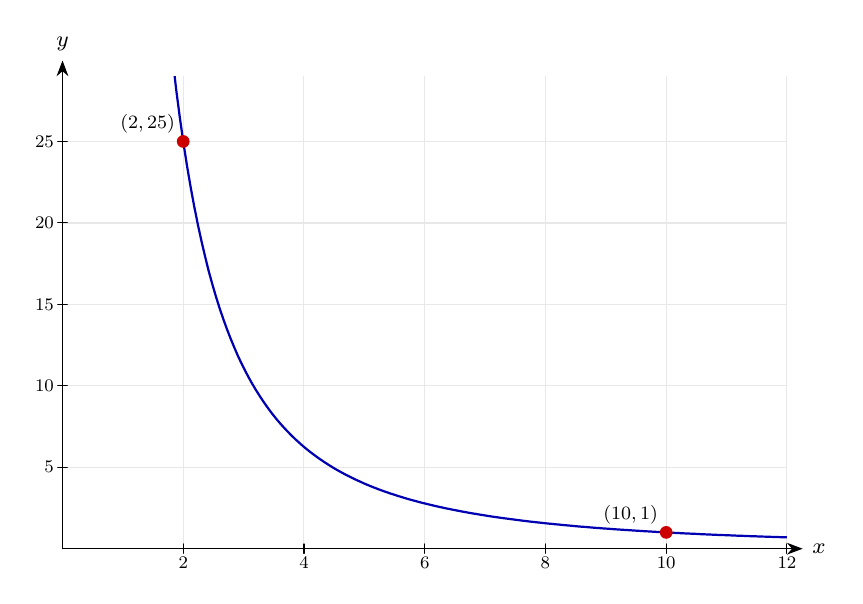
\begin{tikzpicture}[>={Stealth[length=2mm]},font=\footnotesize,line cap=round,line join=round]
\begin{scope}
\clip (0,0) rectangle (9.2,6);
\draw[gray!18] (0,0) grid[xstep=1.533,ystep=1.034] (9.2,6);
\draw[blue!70!black,thick] (0.023,12) -- (0.069,12) -- (0.115,12) -- (0.161,12) -- (0.207,12) -- (0.252,12) -- (0.298,12) -- (0.344,12) -- (0.39,12) -- (0.436,12) -- (0.482,12) -- (0.528,12) -- (0.574,12) -- (0.62,12) -- (0.665,12) -- (0.711,12) -- (0.757,12) -- (0.803,12) -- (0.849,12) -- (0.895,12) -- (0.941,12) -- (0.987,12) -- (1.032,11.408) -- (1.078,10.458) -- (1.124,9.622) -- (1.17,8.882) -- (1.216,8.224) -- (1.262,7.637) -- (1.308,7.11) -- (1.354,6.637) -- (1.4,6.209) -- (1.445,5.821) -- (1.491,5.468) -- (1.537,5.146) -- (1.583,4.852) -- (1.629,4.583) -- (1.675,4.335) -- (1.721,4.107) -- (1.767,3.897) -- (1.813,3.702) -- (1.858,3.521) -- (1.904,3.354) -- (1.95,3.198) -- (1.996,3.052) -- (2.042,2.917) -- (2.088,2.79) -- (2.134,2.671) -- (2.18,2.56) -- (2.225,2.455) -- (2.271,2.357) -- (2.317,2.265) -- (2.363,2.178) -- (2.409,2.095) -- (2.455,2.018) -- (2.501,1.945) -- (2.547,1.875) -- (2.593,1.809) -- (2.638,1.747) -- (2.684,1.688) -- (2.73,1.631) -- (2.776,1.578) -- (2.822,1.527) -- (2.868,1.479) -- (2.914,1.432) -- (2.96,1.388) -- (3.006,1.346) -- (3.051,1.306) -- (3.097,1.268) -- (3.143,1.231) -- (3.189,1.196) -- (3.235,1.162) -- (3.281,1.13) -- (3.327,1.099) -- (3.373,1.069) -- (3.418,1.041) -- (3.464,1.013) -- (3.51,0.987) -- (3.556,0.962) -- (3.602,0.937) -- (3.648,0.914) -- (3.694,0.891) -- (3.74,0.87) -- (3.786,0.849) -- (3.831,0.828) -- (3.877,0.809) -- (3.923,0.79) -- (3.969,0.772) -- (4.015,0.754) -- (4.061,0.737) -- (4.107,0.721) -- (4.153,0.705) -- (4.199,0.69) -- (4.244,0.675) -- (4.29,0.661) -- (4.336,0.647) -- (4.382,0.633) -- (4.428,0.62) -- (4.474,0.608) -- (4.52,0.595) -- (4.566,0.583) -- (4.612,0.572) -- (4.657,0.561) -- (4.703,0.55) -- (4.749,0.539) -- (4.795,0.529) -- (4.841,0.519) -- (4.887,0.509) -- (4.933,0.5) -- (4.979,0.491) -- (5.024,0.482) -- (5.07,0.473) -- (5.116,0.465) -- (5.162,0.456) -- (5.208,0.448) -- (5.254,0.441) -- (5.3,0.433) -- (5.346,0.426) -- (5.392,0.418) -- (5.437,0.411) -- (5.483,0.404) -- (5.529,0.398) -- (5.575,0.391) -- (5.621,0.385) -- (5.667,0.379) -- (5.713,0.373) -- (5.759,0.367) -- (5.805,0.361) -- (5.85,0.355) -- (5.896,0.35) -- (5.942,0.344) -- (5.988,0.339) -- (6.034,0.334) -- (6.08,0.329) -- (6.126,0.324) -- (6.172,0.319) -- (6.217,0.315) -- (6.263,0.31) -- (6.309,0.306) -- (6.355,0.301) -- (6.401,0.297) -- (6.447,0.293) -- (6.493,0.288) -- (6.539,0.284) -- (6.585,0.28) -- (6.63,0.277) -- (6.676,0.273) -- (6.722,0.269) -- (6.768,0.265) -- (6.814,0.262) -- (6.86,0.258) -- (6.906,0.255) -- (6.952,0.252) -- (6.998,0.248) -- (7.043,0.245) -- (7.089,0.242) -- (7.135,0.239) -- (7.181,0.236) -- (7.227,0.233) -- (7.273,0.23) -- (7.319,0.227) -- (7.365,0.224) -- (7.41,0.221) -- (7.456,0.219) -- (7.502,0.216) -- (7.548,0.213) -- (7.594,0.211) -- (7.64,0.208) -- (7.686,0.206) -- (7.732,0.203) -- (7.778,0.201) -- (7.823,0.199) -- (7.869,0.196) -- (7.915,0.194) -- (7.961,0.192) -- (8.007,0.19) -- (8.053,0.188) -- (8.099,0.185) -- (8.145,0.183) -- (8.191,0.181) -- (8.236,0.179) -- (8.282,0.177) -- (8.328,0.175) -- (8.374,0.173) -- (8.42,0.172) -- (8.466,0.17) -- (8.512,0.168) -- (8.558,0.166) -- (8.603,0.164) -- (8.649,0.163) -- (8.695,0.161) -- (8.741,0.159) -- (8.787,0.158) -- (8.833,0.156) -- (8.879,0.154) -- (8.925,0.153) -- (8.971,0.151) -- (9.016,0.15) -- (9.062,0.148) -- (9.108,0.147) -- (9.154,0.145) -- (9.2,0.144);
\end{scope}
\draw[->] (0,0) -- (9.4,0) node[right]{$x$};
\draw[->] (0,0) -- (0,6.2) node[above]{$y$};
\draw (1.533,-0.06) -- (1.533,0.06) node[below=2pt,scale=0.8]{$2$};
\draw (3.067,-0.06) -- (3.067,0.06) node[below=2pt,scale=0.8]{$4$};
\draw (4.6,-0.06) -- (4.6,0.06) node[below=2pt,scale=0.8]{$6$};
\draw (6.133,-0.06) -- (6.133,0.06) node[below=2pt,scale=0.8]{$8$};
\draw (7.667,-0.06) -- (7.667,0.06) node[below=2pt,scale=0.8]{$10$};
\draw (9.2,-0.06) -- (9.2,0.06) node[below=2pt,scale=0.8]{$12$};
\draw (-0.06,1.034) -- (0.06,1.034) node[left=2pt,scale=0.8]{$5$};
\draw (-0.06,2.069) -- (0.06,2.069) node[left=2pt,scale=0.8]{$10$};
\draw (-0.06,3.103) -- (0.06,3.103) node[left=2pt,scale=0.8]{$15$};
\draw (-0.06,4.138) -- (0.06,4.138) node[left=2pt,scale=0.8]{$20$};
\draw (-0.06,5.172) -- (0.06,5.172) node[left=2pt,scale=0.8]{$25$};
\fill[red!80!black] (1.533,5.172) circle (2.3pt);
\node[above left,scale=0.85] at (1.533,5.172) {$(2,25)$};
\fill[red!80!black] (7.667,0.207) circle (2.3pt);
\node[above left,scale=0.85] at (7.667,0.207) {$(10,1)$};
\end{tikzpicture}
}
\end{center}
\small The relationship plotted, with the data points marked.\normalsize

\medskip\hrule

\section*{Proportion 25\quad\small\texttt{(cg4-025)}}
\addcontentsline{toc}{section}{Proportion 25 (cg4-025)}
\textit{Difficulty: Foundation \quad\textbar\quad Marks: 5}

\question{The gravitational force \( F \) N between two objects is inversely proportional to the square of the distance \( r \) m between them. When \( r = 3 \) m, \( F = 20 \) N. Find the force when \( r = 6 \) m, and hence state the effect of tripling the original distance on the force.}

\textbf{Worked solution.}

\textit{Step 1: Write \( F = \frac{k}{r^2} \) and find \( k \).}
\[\begin{gathered}
20 = \frac{k}{9} \implies k = 180
\end{gathered}\]
Multiply both sides by 9.

\textit{Step 2: Find \( F \) when \( r = 6 \).}
\[\begin{gathered}
F = \frac{180}{36} = 5 \text{ N}
\end{gathered}\]
The force is 5 N when the distance is 6 m.

\textit{Step 3: State the effect of tripling the distance (\( r \to 3r \)).}
\[\begin{gathered}
F_{\text{new}} = \frac{k}{(3r)^2} = \frac{k}{9r^2} = \frac{F_{\text{old}}}{9}
\end{gathered}\]
Tripling the distance reduces the force by a factor of 9.

\begin{answerbox}
\textbf{Final answer:}\quad \(\displaystyle  F = 5 \) N when \(\displaystyle  r = 6 \) m; tripling the distance reduces the force to \(\displaystyle  \frac{1}{9} \) of its original value.
\end{answerbox}
\textbf{Graph.}

\begin{center}
\resizebox{\ifdim\width>\linewidth \linewidth\else \width\fi}{!}{%
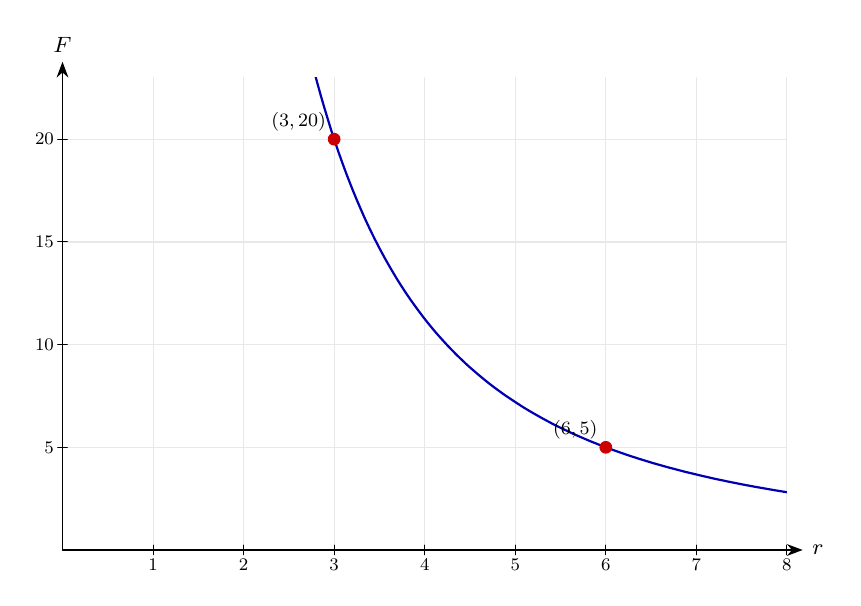
\begin{tikzpicture}[>={Stealth[length=2mm]},font=\footnotesize,line cap=round,line join=round]
\begin{scope}
\clip (0,0) rectangle (9.2,6);
\draw[gray!18] (0,0) grid[xstep=1.15,ystep=1.304] (9.2,6);
\draw[blue!70!black,thick] (0.023,12) -- (0.069,12) -- (0.115,12) -- (0.161,12) -- (0.207,12) -- (0.252,12) -- (0.298,12) -- (0.344,12) -- (0.39,12) -- (0.436,12) -- (0.482,12) -- (0.528,12) -- (0.574,12) -- (0.62,12) -- (0.665,12) -- (0.711,12) -- (0.757,12) -- (0.803,12) -- (0.849,12) -- (0.895,12) -- (0.941,12) -- (0.987,12) -- (1.032,12) -- (1.078,12) -- (1.124,12) -- (1.17,12) -- (1.216,12) -- (1.262,12) -- (1.308,12) -- (1.354,12) -- (1.4,12) -- (1.445,12) -- (1.491,12) -- (1.537,12) -- (1.583,12) -- (1.629,12) -- (1.675,12) -- (1.721,12) -- (1.767,12) -- (1.813,12) -- (1.858,12) -- (1.904,12) -- (1.95,12) -- (1.996,12) -- (2.042,12) -- (2.088,12) -- (2.134,12) -- (2.18,12) -- (2.225,12) -- (2.271,12) -- (2.317,11.565) -- (2.363,11.12) -- (2.409,10.701) -- (2.455,10.304) -- (2.501,9.93) -- (2.547,9.575) -- (2.593,9.239) -- (2.638,8.921) -- (2.684,8.618) -- (2.73,8.331) -- (2.776,8.058) -- (2.822,7.798) -- (2.868,7.55) -- (2.914,7.315) -- (2.96,7.089) -- (3.006,6.875) -- (3.051,6.669) -- (3.097,6.473) -- (3.143,6.286) -- (3.189,6.106) -- (3.235,5.934) -- (3.281,5.769) -- (3.327,5.611) -- (3.373,5.46) -- (3.418,5.314) -- (3.464,5.174) -- (3.51,5.04) -- (3.556,4.911) -- (3.602,4.786) -- (3.648,4.667) -- (3.694,4.551) -- (3.74,4.44) -- (3.786,4.333) -- (3.831,4.23) -- (3.877,4.131) -- (3.923,4.035) -- (3.969,3.942) -- (4.015,3.852) -- (4.061,3.766) -- (4.107,3.682) -- (4.153,3.601) -- (4.199,3.523) -- (4.244,3.447) -- (4.29,3.374) -- (4.336,3.303) -- (4.382,3.234) -- (4.428,3.167) -- (4.474,3.103) -- (4.52,3.04) -- (4.566,2.979) -- (4.611,2.92) -- (4.657,2.863) -- (4.703,2.807) -- (4.749,2.753) -- (4.795,2.701) -- (4.841,2.65) -- (4.887,2.6) -- (4.933,2.552) -- (4.979,2.505) -- (5.024,2.46) -- (5.07,2.416) -- (5.116,2.372) -- (5.162,2.33) -- (5.208,2.29) -- (5.254,2.25) -- (5.3,2.211) -- (5.346,2.173) -- (5.392,2.136) -- (5.437,2.1) -- (5.483,2.065) -- (5.529,2.031) -- (5.575,1.998) -- (5.621,1.965) -- (5.667,1.934) -- (5.713,1.903) -- (5.759,1.873) -- (5.805,1.843) -- (5.85,1.814) -- (5.896,1.786) -- (5.942,1.759) -- (5.988,1.732) -- (6.034,1.706) -- (6.08,1.68) -- (6.126,1.655) -- (6.172,1.63) -- (6.217,1.606) -- (6.263,1.583) -- (6.309,1.56) -- (6.355,1.538) -- (6.401,1.516) -- (6.447,1.494) -- (6.493,1.473) -- (6.539,1.452) -- (6.585,1.432) -- (6.63,1.413) -- (6.676,1.393) -- (6.722,1.374) -- (6.768,1.356) -- (6.814,1.337) -- (6.86,1.32) -- (6.906,1.302) -- (6.952,1.285) -- (6.998,1.268) -- (7.043,1.252) -- (7.089,1.236) -- (7.135,1.22) -- (7.181,1.204) -- (7.227,1.189) -- (7.273,1.174) -- (7.319,1.159) -- (7.365,1.145) -- (7.41,1.131) -- (7.456,1.117) -- (7.502,1.103) -- (7.548,1.09) -- (7.594,1.077) -- (7.64,1.064) -- (7.686,1.051) -- (7.732,1.039) -- (7.778,1.027) -- (7.823,1.015) -- (7.869,1.003) -- (7.915,0.991) -- (7.961,0.98) -- (8.007,0.969) -- (8.053,0.958) -- (8.099,0.947) -- (8.145,0.936) -- (8.191,0.926) -- (8.236,0.915) -- (8.282,0.905) -- (8.328,0.895) -- (8.374,0.886) -- (8.42,0.876) -- (8.466,0.866) -- (8.512,0.857) -- (8.558,0.848) -- (8.603,0.839) -- (8.649,0.83) -- (8.695,0.821) -- (8.741,0.813) -- (8.787,0.804) -- (8.833,0.796) -- (8.879,0.788) -- (8.925,0.78) -- (8.971,0.772) -- (9.016,0.764) -- (9.062,0.756) -- (9.108,0.749) -- (9.154,0.741) -- (9.2,0.734);
\end{scope}
\draw[->] (0,0) -- (9.4,0) node[right]{$r$};
\draw[->] (0,0) -- (0,6.2) node[above]{$F$};
\draw (1.15,-0.06) -- (1.15,0.06) node[below=2pt,scale=0.8]{$1$};
\draw (2.3,-0.06) -- (2.3,0.06) node[below=2pt,scale=0.8]{$2$};
\draw (3.45,-0.06) -- (3.45,0.06) node[below=2pt,scale=0.8]{$3$};
\draw (4.6,-0.06) -- (4.6,0.06) node[below=2pt,scale=0.8]{$4$};
\draw (5.75,-0.06) -- (5.75,0.06) node[below=2pt,scale=0.8]{$5$};
\draw (6.9,-0.06) -- (6.9,0.06) node[below=2pt,scale=0.8]{$6$};
\draw (8.05,-0.06) -- (8.05,0.06) node[below=2pt,scale=0.8]{$7$};
\draw (9.2,-0.06) -- (9.2,0.06) node[below=2pt,scale=0.8]{$8$};
\draw (-0.06,1.304) -- (0.06,1.304) node[left=2pt,scale=0.8]{$5$};
\draw (-0.06,2.609) -- (0.06,2.609) node[left=2pt,scale=0.8]{$10$};
\draw (-0.06,3.913) -- (0.06,3.913) node[left=2pt,scale=0.8]{$15$};
\draw (-0.06,5.217) -- (0.06,5.217) node[left=2pt,scale=0.8]{$20$};
\fill[red!80!black] (3.45,5.217) circle (2.3pt);
\node[above left,scale=0.85] at (3.45,5.217) {$(3,20)$};
\fill[red!80!black] (6.9,1.304) circle (2.3pt);
\node[above left,scale=0.85] at (6.9,1.304) {$(6,5)$};
\end{tikzpicture}
}
\end{center}
\small The relationship plotted, with the data points marked.\normalsize

\medskip\hrule

\section*{Proportion 26\quad\small\texttt{(cg4-026)}}
\addcontentsline{toc}{section}{Proportion 26 (cg4-026)}
\textit{Difficulty: Foundation \quad\textbar\quad Marks: 3}

\question{Given that \( y \propto \dfrac{1}{x^2} \), \( y = 9 \) when \( x = 4 \), and \( y = a \) when \( x = 12 \), find \( a \).}

\textbf{Worked solution.}

\textit{Step 1: Find \( k \).}
\[\begin{gathered}
k = 9 \times 16 = 144
\end{gathered}\]
\( k = y \cdot x^2 = 9 \times 4^2 \).

\textit{Step 2: Substitute \( x = 12 \).}
\[\begin{gathered}
a = \frac{144}{144} = 1
\end{gathered}\]
\( 12^2 = 144 \), so \( a = \frac{144}{144} = 1 \).

\begin{answerbox}
\textbf{Final answer:}\quad \(\displaystyle  a = 1 \)
\end{answerbox}
\textbf{Graph.}

\begin{center}
\resizebox{\ifdim\width>\linewidth \linewidth\else \width\fi}{!}{%
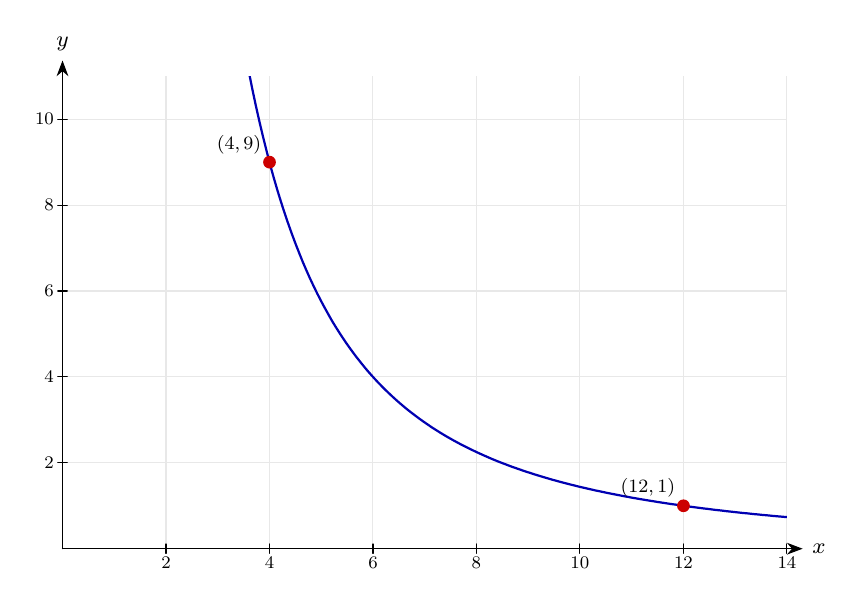
\begin{tikzpicture}[>={Stealth[length=2mm]},font=\footnotesize,line cap=round,line join=round]
\begin{scope}
\clip (0,0) rectangle (9.2,6);
\draw[gray!18] (0,0) grid[xstep=1.314,ystep=1.091] (9.2,6);
\draw[blue!70!black,thick] (0.023,12) -- (0.069,12) -- (0.115,12) -- (0.161,12) -- (0.207,12) -- (0.252,12) -- (0.298,12) -- (0.344,12) -- (0.39,12) -- (0.436,12) -- (0.482,12) -- (0.528,12) -- (0.574,12) -- (0.62,12) -- (0.665,12) -- (0.711,12) -- (0.757,12) -- (0.803,12) -- (0.849,12) -- (0.895,12) -- (0.941,12) -- (0.987,12) -- (1.032,12) -- (1.078,12) -- (1.124,12) -- (1.17,12) -- (1.216,12) -- (1.262,12) -- (1.308,12) -- (1.354,12) -- (1.4,12) -- (1.445,12) -- (1.491,12) -- (1.537,12) -- (1.583,12) -- (1.629,12) -- (1.675,12) -- (1.721,11.455) -- (1.767,10.868) -- (1.813,10.325) -- (1.858,9.821) -- (1.904,9.354) -- (1.95,8.919) -- (1.996,8.513) -- (2.042,8.135) -- (2.088,7.781) -- (2.134,7.45) -- (2.18,7.14) -- (2.225,6.848) -- (2.271,6.575) -- (2.317,6.317) -- (2.363,6.074) -- (2.409,5.845) -- (2.455,5.628) -- (2.501,5.424) -- (2.547,5.23) -- (2.593,5.046) -- (2.638,4.872) -- (2.684,4.707) -- (2.73,4.55) -- (2.776,4.401) -- (2.822,4.259) -- (2.868,4.124) -- (2.914,3.995) -- (2.96,3.872) -- (3.006,3.755) -- (3.051,3.643) -- (3.097,3.536) -- (3.143,3.433) -- (3.189,3.335) -- (3.235,3.241) -- (3.281,3.151) -- (3.327,3.065) -- (3.373,2.982) -- (3.418,2.902) -- (3.464,2.826) -- (3.51,2.753) -- (3.556,2.682) -- (3.602,2.614) -- (3.648,2.549) -- (3.694,2.486) -- (3.74,2.425) -- (3.786,2.367) -- (3.831,2.311) -- (3.877,2.256) -- (3.923,2.204) -- (3.969,2.153) -- (4.015,2.104) -- (4.061,2.057) -- (4.107,2.011) -- (4.153,1.967) -- (4.199,1.924) -- (4.244,1.883) -- (4.29,1.843) -- (4.336,1.804) -- (4.382,1.766) -- (4.428,1.73) -- (4.474,1.695) -- (4.52,1.66) -- (4.566,1.627) -- (4.612,1.595) -- (4.657,1.564) -- (4.703,1.533) -- (4.749,1.504) -- (4.795,1.475) -- (4.841,1.447) -- (4.887,1.42) -- (4.933,1.394) -- (4.979,1.368) -- (5.024,1.344) -- (5.07,1.319) -- (5.116,1.296) -- (5.162,1.273) -- (5.208,1.251) -- (5.254,1.229) -- (5.3,1.208) -- (5.346,1.187) -- (5.392,1.167) -- (5.437,1.147) -- (5.483,1.128) -- (5.529,1.109) -- (5.575,1.091) -- (5.621,1.074) -- (5.667,1.056) -- (5.713,1.039) -- (5.759,1.023) -- (5.805,1.007) -- (5.85,0.991) -- (5.896,0.976) -- (5.942,0.961) -- (5.988,0.946) -- (6.034,0.932) -- (6.08,0.918) -- (6.126,0.904) -- (6.172,0.891) -- (6.217,0.877) -- (6.263,0.865) -- (6.309,0.852) -- (6.355,0.84) -- (6.401,0.828) -- (6.447,0.816) -- (6.493,0.805) -- (6.539,0.793) -- (6.585,0.782) -- (6.63,0.772) -- (6.676,0.761) -- (6.722,0.751) -- (6.768,0.74) -- (6.814,0.731) -- (6.86,0.721) -- (6.906,0.711) -- (6.952,0.702) -- (6.998,0.693) -- (7.043,0.684) -- (7.089,0.675) -- (7.135,0.666) -- (7.181,0.658) -- (7.227,0.649) -- (7.273,0.641) -- (7.319,0.633) -- (7.365,0.625) -- (7.41,0.618) -- (7.456,0.61) -- (7.502,0.603) -- (7.548,0.595) -- (7.594,0.588) -- (7.64,0.581) -- (7.686,0.574) -- (7.732,0.567) -- (7.778,0.561) -- (7.823,0.554) -- (7.869,0.548) -- (7.915,0.541) -- (7.961,0.535) -- (8.007,0.529) -- (8.053,0.523) -- (8.099,0.517) -- (8.145,0.511) -- (8.191,0.506) -- (8.236,0.5) -- (8.282,0.494) -- (8.328,0.489) -- (8.374,0.484) -- (8.42,0.478) -- (8.466,0.473) -- (8.512,0.468) -- (8.558,0.463) -- (8.603,0.458) -- (8.649,0.453) -- (8.695,0.449) -- (8.741,0.444) -- (8.787,0.439) -- (8.833,0.435) -- (8.879,0.43) -- (8.925,0.426) -- (8.971,0.422) -- (9.016,0.417) -- (9.062,0.413) -- (9.108,0.409) -- (9.154,0.405) -- (9.2,0.401);
\end{scope}
\draw[->] (0,0) -- (9.4,0) node[right]{$x$};
\draw[->] (0,0) -- (0,6.2) node[above]{$y$};
\draw (1.314,-0.06) -- (1.314,0.06) node[below=2pt,scale=0.8]{$2$};
\draw (2.629,-0.06) -- (2.629,0.06) node[below=2pt,scale=0.8]{$4$};
\draw (3.943,-0.06) -- (3.943,0.06) node[below=2pt,scale=0.8]{$6$};
\draw (5.257,-0.06) -- (5.257,0.06) node[below=2pt,scale=0.8]{$8$};
\draw (6.571,-0.06) -- (6.571,0.06) node[below=2pt,scale=0.8]{$10$};
\draw (7.886,-0.06) -- (7.886,0.06) node[below=2pt,scale=0.8]{$12$};
\draw (9.2,-0.06) -- (9.2,0.06) node[below=2pt,scale=0.8]{$14$};
\draw (-0.06,1.091) -- (0.06,1.091) node[left=2pt,scale=0.8]{$2$};
\draw (-0.06,2.182) -- (0.06,2.182) node[left=2pt,scale=0.8]{$4$};
\draw (-0.06,3.273) -- (0.06,3.273) node[left=2pt,scale=0.8]{$6$};
\draw (-0.06,4.364) -- (0.06,4.364) node[left=2pt,scale=0.8]{$8$};
\draw (-0.06,5.455) -- (0.06,5.455) node[left=2pt,scale=0.8]{$10$};
\fill[red!80!black] (2.629,4.909) circle (2.3pt);
\node[above left,scale=0.85] at (2.629,4.909) {$(4,9)$};
\fill[red!80!black] (7.886,0.545) circle (2.3pt);
\node[above left,scale=0.85] at (7.886,0.545) {$(12,1)$};
\end{tikzpicture}
}
\end{center}
\small The relationship plotted, with the data points marked.\normalsize

\medskip\hrule

\section*{Proportion 27\quad\small\texttt{(cg4-027)}}
\addcontentsline{toc}{section}{Proportion 27 (cg4-027)}
\textit{Difficulty: Foundation \quad\textbar\quad Marks: 3}

\question{Given that \( y \propto \sqrt{x} \) and that \( y = 15 \) when \( x = 25 \), find \( y \) when \( x = 64 \).}

\textbf{Worked solution.}

\textit{Step 1: Write \( y = k\sqrt{x} \) and find \( k \).}
\[\begin{gathered}
15 = k\sqrt{25} = 5k \implies k = 3
\end{gathered}\]
\( \sqrt{25} = 5 \); divide both sides by 5.

\textit{Step 2: Substitute \( x = 64 \).}
\[\begin{gathered}
y = 3\sqrt{64} = 3 \times 8 = 24
\end{gathered}\]
\( \sqrt{64} = 8 \).

\begin{answerbox}
\textbf{Final answer:}\quad \(\displaystyle  y = 24 \)
\end{answerbox}
\textbf{Graph.}

\begin{center}
\resizebox{\ifdim\width>\linewidth \linewidth\else \width\fi}{!}{%
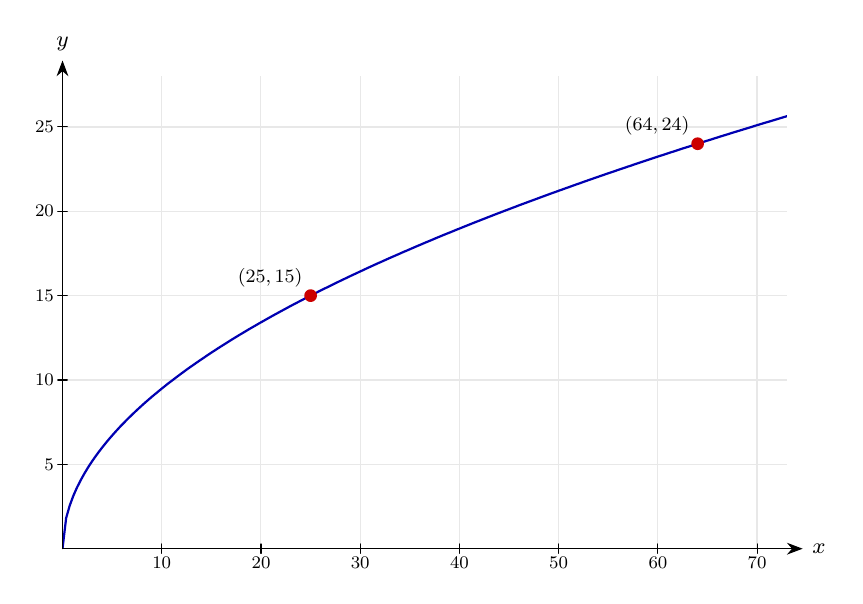
\begin{tikzpicture}[>={Stealth[length=2mm]},font=\footnotesize,line cap=round,line join=round]
\begin{scope}
\clip (0,0) rectangle (9.2,6);
\draw[gray!18] (0,0) grid[xstep=1.26,ystep=1.071] (9.2,6);
\draw[blue!70!black,thick] (0,0) -- (0.046,0.388) -- (0.092,0.549) -- (0.138,0.673) -- (0.184,0.777) -- (0.23,0.868) -- (0.276,0.951) -- (0.322,1.028) -- (0.368,1.099) -- (0.414,1.165) -- (0.46,1.228) -- (0.506,1.288) -- (0.552,1.345) -- (0.598,1.4) -- (0.644,1.453) -- (0.69,1.504) -- (0.736,1.554) -- (0.782,1.601) -- (0.828,1.648) -- (0.874,1.693) -- (0.92,1.737) -- (0.966,1.78) -- (1.012,1.822) -- (1.058,1.863) -- (1.104,1.903) -- (1.15,1.942) -- (1.196,1.98) -- (1.242,2.018) -- (1.288,2.055) -- (1.334,2.092) -- (1.38,2.127) -- (1.426,2.162) -- (1.472,2.197) -- (1.518,2.231) -- (1.564,2.265) -- (1.61,2.298) -- (1.656,2.33) -- (1.702,2.362) -- (1.748,2.394) -- (1.794,2.425) -- (1.84,2.456) -- (1.886,2.487) -- (1.932,2.517) -- (1.978,2.547) -- (2.024,2.576) -- (2.07,2.605) -- (2.116,2.634) -- (2.162,2.663) -- (2.208,2.691) -- (2.254,2.719) -- (2.3,2.746) -- (2.346,2.774) -- (2.392,2.801) -- (2.438,2.827) -- (2.484,2.854) -- (2.53,2.88) -- (2.576,2.906) -- (2.622,2.932) -- (2.668,2.958) -- (2.714,2.983) -- (2.76,3.008) -- (2.806,3.033) -- (2.852,3.058) -- (2.898,3.083) -- (2.944,3.107) -- (2.99,3.131) -- (3.036,3.155) -- (3.082,3.179) -- (3.128,3.203) -- (3.174,3.226) -- (3.22,3.249) -- (3.266,3.273) -- (3.312,3.296) -- (3.358,3.318) -- (3.404,3.341) -- (3.45,3.364) -- (3.496,3.386) -- (3.542,3.408) -- (3.588,3.43) -- (3.634,3.452) -- (3.68,3.474) -- (3.726,3.495) -- (3.772,3.517) -- (3.818,3.538) -- (3.864,3.56) -- (3.91,3.581) -- (3.956,3.602) -- (4.002,3.623) -- (4.048,3.643) -- (4.094,3.664) -- (4.14,3.685) -- (4.186,3.705) -- (4.232,3.725) -- (4.278,3.745) -- (4.324,3.766) -- (4.37,3.785) -- (4.416,3.805) -- (4.462,3.825) -- (4.508,3.845) -- (4.554,3.864) -- (4.6,3.884) -- (4.646,3.903) -- (4.692,3.922) -- (4.738,3.942) -- (4.784,3.961) -- (4.83,3.98) -- (4.876,3.999) -- (4.922,4.017) -- (4.968,4.036) -- (5.014,4.055) -- (5.06,4.073) -- (5.106,4.092) -- (5.152,4.11) -- (5.198,4.129) -- (5.244,4.147) -- (5.29,4.165) -- (5.336,4.183) -- (5.382,4.201) -- (5.428,4.219) -- (5.474,4.237) -- (5.52,4.255) -- (5.566,4.272) -- (5.612,4.29) -- (5.658,4.307) -- (5.704,4.325) -- (5.75,4.342) -- (5.796,4.36) -- (5.842,4.377) -- (5.888,4.394) -- (5.934,4.411) -- (5.98,4.428) -- (6.026,4.445) -- (6.072,4.462) -- (6.118,4.479) -- (6.164,4.496) -- (6.21,4.513) -- (6.256,4.529) -- (6.302,4.546) -- (6.348,4.562) -- (6.394,4.579) -- (6.44,4.595) -- (6.486,4.612) -- (6.532,4.628) -- (6.578,4.644) -- (6.624,4.661) -- (6.67,4.677) -- (6.716,4.693) -- (6.762,4.709) -- (6.808,4.725) -- (6.854,4.741) -- (6.9,4.757) -- (6.946,4.773) -- (6.992,4.788) -- (7.038,4.804) -- (7.084,4.82) -- (7.13,4.835) -- (7.176,4.851) -- (7.222,4.866) -- (7.268,4.882) -- (7.314,4.897) -- (7.36,4.913) -- (7.406,4.928) -- (7.452,4.943) -- (7.498,4.959) -- (7.544,4.974) -- (7.59,4.989) -- (7.636,5.004) -- (7.682,5.019) -- (7.728,5.034) -- (7.774,5.049) -- (7.82,5.064) -- (7.866,5.079) -- (7.912,5.094) -- (7.958,5.108) -- (8.004,5.123) -- (8.05,5.138) -- (8.096,5.152) -- (8.142,5.167) -- (8.188,5.182) -- (8.234,5.196) -- (8.28,5.211) -- (8.326,5.225) -- (8.372,5.24) -- (8.418,5.254) -- (8.464,5.268) -- (8.51,5.283) -- (8.556,5.297) -- (8.602,5.311) -- (8.648,5.325) -- (8.694,5.339) -- (8.74,5.353) -- (8.786,5.368) -- (8.832,5.382) -- (8.878,5.396) -- (8.924,5.41) -- (8.97,5.423) -- (9.016,5.437) -- (9.062,5.451) -- (9.108,5.465) -- (9.154,5.479) -- (9.2,5.493);
\end{scope}
\draw[->] (0,0) -- (9.4,0) node[right]{$x$};
\draw[->] (0,0) -- (0,6.2) node[above]{$y$};
\draw (1.26,-0.06) -- (1.26,0.06) node[below=2pt,scale=0.8]{$10$};
\draw (2.521,-0.06) -- (2.521,0.06) node[below=2pt,scale=0.8]{$20$};
\draw (3.781,-0.06) -- (3.781,0.06) node[below=2pt,scale=0.8]{$30$};
\draw (5.041,-0.06) -- (5.041,0.06) node[below=2pt,scale=0.8]{$40$};
\draw (6.301,-0.06) -- (6.301,0.06) node[below=2pt,scale=0.8]{$50$};
\draw (7.562,-0.06) -- (7.562,0.06) node[below=2pt,scale=0.8]{$60$};
\draw (8.822,-0.06) -- (8.822,0.06) node[below=2pt,scale=0.8]{$70$};
\draw (-0.06,1.071) -- (0.06,1.071) node[left=2pt,scale=0.8]{$5$};
\draw (-0.06,2.143) -- (0.06,2.143) node[left=2pt,scale=0.8]{$10$};
\draw (-0.06,3.214) -- (0.06,3.214) node[left=2pt,scale=0.8]{$15$};
\draw (-0.06,4.286) -- (0.06,4.286) node[left=2pt,scale=0.8]{$20$};
\draw (-0.06,5.357) -- (0.06,5.357) node[left=2pt,scale=0.8]{$25$};
\fill[red!80!black] (3.151,3.214) circle (2.3pt);
\node[above left,scale=0.85] at (3.151,3.214) {$(25,15)$};
\fill[red!80!black] (8.066,5.143) circle (2.3pt);
\node[above left,scale=0.85] at (8.066,5.143) {$(64,24)$};
\end{tikzpicture}
}
\end{center}
\small The relationship plotted, with the data points marked.\normalsize

\medskip\hrule

\section*{Proportion 28\quad\small\texttt{(cg4-028)}}
\addcontentsline{toc}{section}{Proportion 28 (cg4-028)}
\textit{Difficulty: Foundation \quad\textbar\quad Marks: 4}

\question{Given that \( y \propto \sqrt{x} \) and \( y = 6 \) when \( x = 9 \), find the exact value of \( x \) when \( y = 10 \).}

\textbf{Worked solution.}

\textit{Step 1: Find \( k \).}
\[\begin{gathered}
6 = k\sqrt{9} = 3k \implies k = 2
\end{gathered}\]
Divide both sides by \( \sqrt{9} = 3 \).

\textit{Step 2: Substitute \( y = 10 \).}
\[\begin{gathered}
10 = 2\sqrt{x} \implies \sqrt{x} = 5
\end{gathered}\]
Divide both sides by 2.

\textit{Step 3: Square both sides.}
\[\begin{gathered}
x = 25
\end{gathered}\]
\( (\sqrt{x})^2 = x \).

\begin{answerbox}
\textbf{Final answer:}\quad \(\displaystyle  x = 25 \)
\end{answerbox}
\textbf{Graph.}

\begin{center}
\resizebox{\ifdim\width>\linewidth \linewidth\else \width\fi}{!}{%
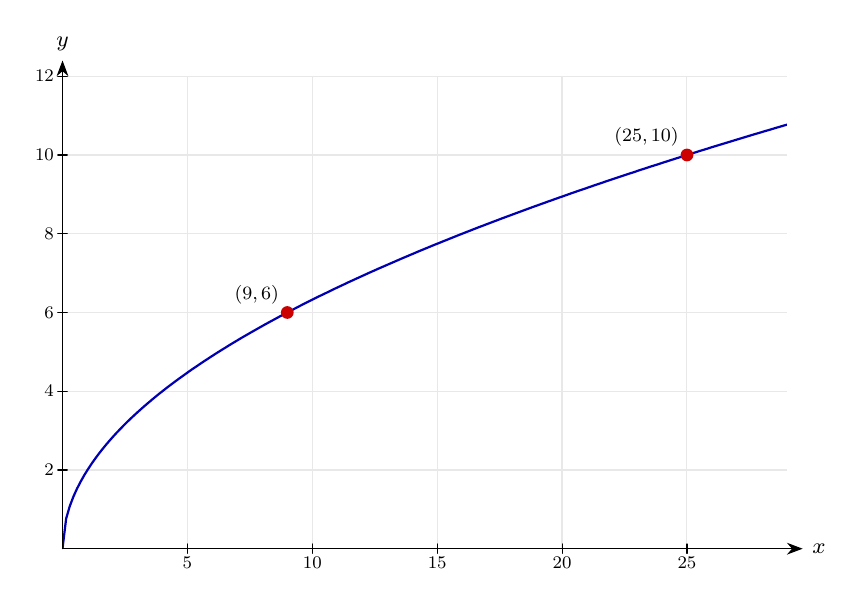
\begin{tikzpicture}[>={Stealth[length=2mm]},font=\footnotesize,line cap=round,line join=round]
\begin{scope}
\clip (0,0) rectangle (9.2,6);
\draw[gray!18] (0,0) grid[xstep=1.586,ystep=1] (9.2,6);
\draw[blue!70!black,thick] (0,0) -- (0.046,0.381) -- (0.092,0.539) -- (0.138,0.66) -- (0.184,0.762) -- (0.23,0.851) -- (0.276,0.933) -- (0.322,1.007) -- (0.368,1.077) -- (0.414,1.142) -- (0.46,1.204) -- (0.506,1.263) -- (0.552,1.319) -- (0.598,1.373) -- (0.644,1.425) -- (0.69,1.475) -- (0.736,1.523) -- (0.782,1.57) -- (0.828,1.616) -- (0.874,1.66) -- (0.92,1.703) -- (0.966,1.745) -- (1.012,1.786) -- (1.058,1.826) -- (1.104,1.865) -- (1.15,1.904) -- (1.196,1.942) -- (1.242,1.979) -- (1.288,2.015) -- (1.334,2.051) -- (1.38,2.086) -- (1.426,2.12) -- (1.472,2.154) -- (1.518,2.187) -- (1.564,2.22) -- (1.61,2.253) -- (1.656,2.285) -- (1.702,2.316) -- (1.748,2.347) -- (1.794,2.378) -- (1.84,2.408) -- (1.886,2.438) -- (1.932,2.468) -- (1.978,2.497) -- (2.024,2.526) -- (2.07,2.554) -- (2.116,2.583) -- (2.162,2.611) -- (2.208,2.638) -- (2.254,2.666) -- (2.3,2.693) -- (2.346,2.719) -- (2.392,2.746) -- (2.438,2.772) -- (2.484,2.798) -- (2.53,2.824) -- (2.576,2.85) -- (2.622,2.875) -- (2.668,2.9) -- (2.714,2.925) -- (2.76,2.95) -- (2.806,2.974) -- (2.852,2.998) -- (2.898,3.022) -- (2.944,3.046) -- (2.99,3.07) -- (3.036,3.094) -- (3.082,3.117) -- (3.128,3.14) -- (3.174,3.163) -- (3.22,3.186) -- (3.266,3.209) -- (3.312,3.231) -- (3.358,3.253) -- (3.404,3.276) -- (3.45,3.298) -- (3.496,3.32) -- (3.542,3.341) -- (3.588,3.363) -- (3.634,3.385) -- (3.68,3.406) -- (3.726,3.427) -- (3.772,3.448) -- (3.818,3.469) -- (3.864,3.49) -- (3.91,3.511) -- (3.956,3.531) -- (4.002,3.552) -- (4.048,3.572) -- (4.094,3.592) -- (4.14,3.612) -- (4.186,3.632) -- (4.232,3.652) -- (4.278,3.672) -- (4.324,3.692) -- (4.37,3.711) -- (4.416,3.731) -- (4.462,3.75) -- (4.508,3.77) -- (4.554,3.789) -- (4.6,3.808) -- (4.646,3.827) -- (4.692,3.846) -- (4.738,3.865) -- (4.784,3.883) -- (4.83,3.902) -- (4.876,3.92) -- (4.922,3.939) -- (4.968,3.957) -- (5.014,3.976) -- (5.06,3.994) -- (5.106,4.012) -- (5.152,4.03) -- (5.198,4.048) -- (5.244,4.066) -- (5.29,4.084) -- (5.336,4.101) -- (5.382,4.119) -- (5.428,4.136) -- (5.474,4.154) -- (5.52,4.171) -- (5.566,4.189) -- (5.612,4.206) -- (5.658,4.223) -- (5.704,4.24) -- (5.75,4.257) -- (5.796,4.274) -- (5.842,4.291) -- (5.888,4.308) -- (5.934,4.325) -- (5.98,4.342) -- (6.026,4.358) -- (6.072,4.375) -- (6.118,4.391) -- (6.164,4.408) -- (6.21,4.424) -- (6.256,4.441) -- (6.302,4.457) -- (6.348,4.473) -- (6.394,4.489) -- (6.44,4.506) -- (6.486,4.522) -- (6.532,4.538) -- (6.578,4.554) -- (6.624,4.569) -- (6.67,4.585) -- (6.716,4.601) -- (6.762,4.617) -- (6.808,4.632) -- (6.854,4.648) -- (6.9,4.664) -- (6.946,4.679) -- (6.992,4.695) -- (7.038,4.71) -- (7.084,4.725) -- (7.13,4.741) -- (7.176,4.756) -- (7.222,4.771) -- (7.268,4.786) -- (7.314,4.802) -- (7.36,4.817) -- (7.406,4.832) -- (7.452,4.847) -- (7.498,4.862) -- (7.544,4.876) -- (7.59,4.891) -- (7.636,4.906) -- (7.682,4.921) -- (7.728,4.936) -- (7.774,4.95) -- (7.82,4.965) -- (7.866,4.979) -- (7.912,4.994) -- (7.958,5.008) -- (8.004,5.023) -- (8.05,5.037) -- (8.096,5.052) -- (8.142,5.066) -- (8.188,5.08) -- (8.234,5.095) -- (8.28,5.109) -- (8.326,5.123) -- (8.372,5.137) -- (8.418,5.151) -- (8.464,5.165) -- (8.51,5.179) -- (8.556,5.193) -- (8.602,5.207) -- (8.648,5.221) -- (8.694,5.235) -- (8.74,5.249) -- (8.786,5.263) -- (8.832,5.276) -- (8.878,5.29) -- (8.924,5.304) -- (8.97,5.317) -- (9.016,5.331) -- (9.062,5.345) -- (9.108,5.358) -- (9.154,5.372) -- (9.2,5.385);
\end{scope}
\draw[->] (0,0) -- (9.4,0) node[right]{$x$};
\draw[->] (0,0) -- (0,6.2) node[above]{$y$};
\draw (1.586,-0.06) -- (1.586,0.06) node[below=2pt,scale=0.8]{$5$};
\draw (3.172,-0.06) -- (3.172,0.06) node[below=2pt,scale=0.8]{$10$};
\draw (4.759,-0.06) -- (4.759,0.06) node[below=2pt,scale=0.8]{$15$};
\draw (6.345,-0.06) -- (6.345,0.06) node[below=2pt,scale=0.8]{$20$};
\draw (7.931,-0.06) -- (7.931,0.06) node[below=2pt,scale=0.8]{$25$};
\draw (-0.06,1) -- (0.06,1) node[left=2pt,scale=0.8]{$2$};
\draw (-0.06,2) -- (0.06,2) node[left=2pt,scale=0.8]{$4$};
\draw (-0.06,3) -- (0.06,3) node[left=2pt,scale=0.8]{$6$};
\draw (-0.06,4) -- (0.06,4) node[left=2pt,scale=0.8]{$8$};
\draw (-0.06,5) -- (0.06,5) node[left=2pt,scale=0.8]{$10$};
\draw (-0.06,6) -- (0.06,6) node[left=2pt,scale=0.8]{$12$};
\fill[red!80!black] (2.855,3) circle (2.3pt);
\node[above left,scale=0.85] at (2.855,3) {$(9,6)$};
\fill[red!80!black] (7.931,5) circle (2.3pt);
\node[above left,scale=0.85] at (7.931,5) {$(25,10)$};
\end{tikzpicture}
}
\end{center}
\small The relationship plotted, with the data points marked.\normalsize

\medskip\hrule

\section*{Proportion 29\quad\small\texttt{(cg4-029)}}
\addcontentsline{toc}{section}{Proportion 29 (cg4-029)}
\textit{Difficulty: Foundation \quad\textbar\quad Marks: 4}

\question{Prove that if \( y \propto x \) and \( z \propto y^2 \), then \( z \propto x^2 \).}

\textbf{Worked solution.}

\textit{Step 1: Write equations for each proportionality.}
\[\begin{gathered}
y = k_1 x \quad \text{and} \quad z = k_2 y^2
\end{gathered}\]
Replace each \( \propto \) with \( = k \cdot \).

\textit{Step 2: Substitute the expression for \( y \) into the equation for \( z \).}
\[\begin{gathered}
z = k_2 (k_1 x)^2 = k_2 k_1^2 x^2
\end{gathered}\]
Expand the bracket: \( (k_1 x)^2 = k_1^2 x^2 \).

\textit{Step 3: Identify the combined constant.}
\[\begin{gathered}
z = K x^2 \quad \text{where } K = k_1^2 k_2 \text{ is a constant}
\end{gathered}\]
Since \( K \) is a product of constants it is itself a constant, so \( z \propto x^2 \). \( \square \)

\begin{answerbox}
\textbf{Final answer:}\quad Proved: \(\displaystyle  z \propto x^2 \)
\end{answerbox}
\medskip\hrule

\section*{Proportion 30\quad\small\texttt{(cg4-030)}}
\addcontentsline{toc}{section}{Proportion 30 (cg4-030)}
\textit{Difficulty: Foundation \quad\textbar\quad Marks: 4}

\question{Prove that if \( y \propto \dfrac{1}{x} \) and \( z \propto \dfrac{1}{y} \), then \( z \propto x \).}

\textbf{Worked solution.}

\textit{Step 1: Write equations for each relationship.}
\[\begin{gathered}
y = \frac{k_1}{x} \quad \text{and} \quad z = \frac{k_2}{y}
\end{gathered}\]
Express each proportionality as an equation.

\textit{Step 2: Substitute \( y \) into the expression for \( z \).}
\[\begin{gathered}
z = \frac{k_2}{\dfrac{k_1}{x}} = \frac{k_2 x}{k_1}
\end{gathered}\]
Dividing by a fraction is multiplying by its reciprocal.

\textit{Step 3: Write in the form \( z = Kx \).}
\[\begin{gathered}
z = \frac{k_2}{k_1} \cdot x = Kx \quad \text{where } K = \frac{k_2}{k_1}
\end{gathered}\]
Since \( K \) is a constant, \( z \propto x \). \( \square \)

\begin{answerbox}
\textbf{Final answer:}\quad Proved: \(\displaystyle  z \propto x \)
\end{answerbox}
\medskip\hrule

\section*{Proportion 31\quad\small\texttt{(cg4-031)}}
\addcontentsline{toc}{section}{Proportion 31 (cg4-031)}
\textit{Difficulty: Foundation \quad\textbar\quad Marks: 4}

\question{The period \( T \) seconds of a pendulum is directly proportional to the square root of its length \( L \) cm. A pendulum of length 100 cm has a period of 2 s. Find the length needed to give a period of 3 s.}

\textbf{Worked solution.}

\textit{Step 1: Write \( T = k\sqrt{L} \) and find \( k \).}
\[\begin{gathered}
2 = k\sqrt{100} = 10k \implies k = 0.2
\end{gathered}\]
\( \sqrt{100} = 10 \); divide both sides by 10.

\textit{Step 2: Substitute \( T = 3 \) and solve for \( L \).}
\[\begin{gathered}
3 = 0.2\sqrt{L} \implies \sqrt{L} = 15 \implies L = 225 \text{ cm}
\end{gathered}\]
Divide by 0.2 then square both sides.

\begin{answerbox}
\textbf{Final answer:}\quad \(\displaystyle  L = 225 \) cm
\end{answerbox}
\textbf{Graph.}

\begin{center}
\resizebox{\ifdim\width>\linewidth \linewidth\else \width\fi}{!}{%
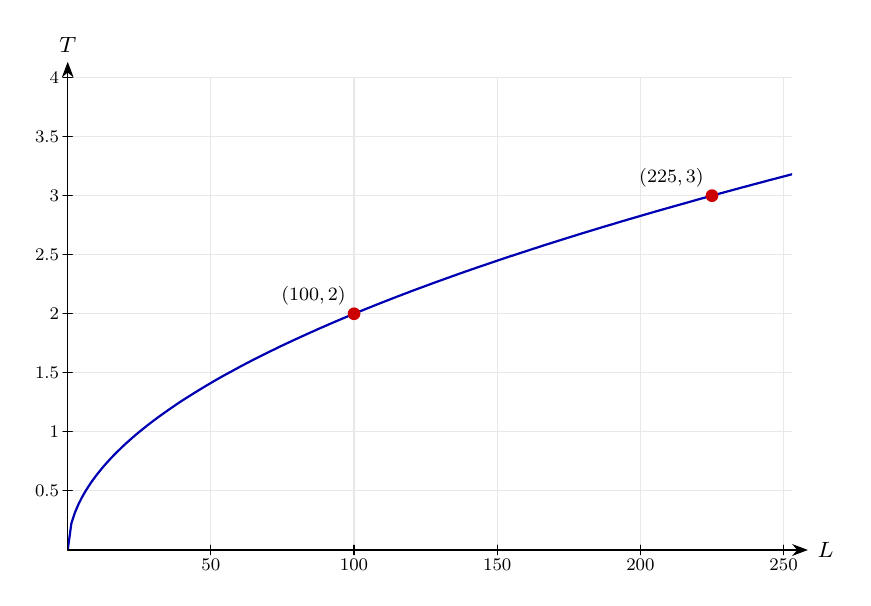
\begin{tikzpicture}[>={Stealth[length=2mm]},font=\footnotesize,line cap=round,line join=round]
\begin{scope}
\clip (0,0) rectangle (9.2,6);
\draw[gray!18] (0,0) grid[xstep=1.818,ystep=0.75] (9.2,6);
\draw[blue!70!black,thick] (0,0) -- (0.046,0.337) -- (0.092,0.477) -- (0.138,0.584) -- (0.184,0.675) -- (0.23,0.754) -- (0.276,0.826) -- (0.322,0.893) -- (0.368,0.954) -- (0.414,1.012) -- (0.46,1.067) -- (0.506,1.119) -- (0.552,1.169) -- (0.598,1.217) -- (0.644,1.262) -- (0.69,1.307) -- (0.736,1.35) -- (0.782,1.391) -- (0.828,1.432) -- (0.874,1.471) -- (0.92,1.509) -- (0.966,1.546) -- (1.012,1.583) -- (1.058,1.618) -- (1.104,1.653) -- (1.15,1.687) -- (1.196,1.72) -- (1.242,1.753) -- (1.288,1.785) -- (1.334,1.817) -- (1.38,1.848) -- (1.426,1.879) -- (1.472,1.909) -- (1.518,1.938) -- (1.564,1.967) -- (1.61,1.996) -- (1.656,2.024) -- (1.702,2.052) -- (1.748,2.08) -- (1.794,2.107) -- (1.84,2.134) -- (1.886,2.161) -- (1.932,2.187) -- (1.978,2.213) -- (2.024,2.238) -- (2.07,2.263) -- (2.116,2.288) -- (2.162,2.313) -- (2.208,2.338) -- (2.254,2.362) -- (2.3,2.386) -- (2.346,2.41) -- (2.392,2.433) -- (2.438,2.456) -- (2.484,2.479) -- (2.53,2.502) -- (2.576,2.525) -- (2.622,2.547) -- (2.668,2.57) -- (2.714,2.592) -- (2.76,2.614) -- (2.806,2.635) -- (2.852,2.657) -- (2.898,2.678) -- (2.944,2.699) -- (2.99,2.72) -- (3.036,2.741) -- (3.082,2.762) -- (3.128,2.782) -- (3.174,2.803) -- (3.22,2.823) -- (3.266,2.843) -- (3.312,2.863) -- (3.358,2.883) -- (3.404,2.903) -- (3.45,2.922) -- (3.496,2.942) -- (3.542,2.961) -- (3.588,2.98) -- (3.634,2.999) -- (3.68,3.018) -- (3.726,3.037) -- (3.772,3.055) -- (3.818,3.074) -- (3.864,3.092) -- (3.91,3.111) -- (3.956,3.129) -- (4.002,3.147) -- (4.048,3.165) -- (4.094,3.183) -- (4.14,3.201) -- (4.186,3.219) -- (4.232,3.236) -- (4.278,3.254) -- (4.324,3.271) -- (4.37,3.289) -- (4.416,3.306) -- (4.462,3.323) -- (4.508,3.34) -- (4.554,3.357) -- (4.6,3.374) -- (4.646,3.391) -- (4.692,3.408) -- (4.738,3.424) -- (4.784,3.441) -- (4.83,3.457) -- (4.876,3.474) -- (4.922,3.49) -- (4.968,3.507) -- (5.014,3.523) -- (5.06,3.539) -- (5.106,3.555) -- (5.152,3.571) -- (5.198,3.587) -- (5.244,3.603) -- (5.29,3.618) -- (5.336,3.634) -- (5.382,3.65) -- (5.428,3.665) -- (5.474,3.681) -- (5.52,3.696) -- (5.566,3.712) -- (5.612,3.727) -- (5.658,3.742) -- (5.704,3.757) -- (5.75,3.772) -- (5.796,3.787) -- (5.842,3.802) -- (5.888,3.817) -- (5.934,3.832) -- (5.98,3.847) -- (6.026,3.862) -- (6.072,3.877) -- (6.118,3.891) -- (6.164,3.906) -- (6.21,3.92) -- (6.256,3.935) -- (6.302,3.949) -- (6.348,3.964) -- (6.394,3.978) -- (6.44,3.992) -- (6.486,4.007) -- (6.532,4.021) -- (6.578,4.035) -- (6.624,4.049) -- (6.67,4.063) -- (6.716,4.077) -- (6.762,4.091) -- (6.808,4.105) -- (6.854,4.119) -- (6.9,4.132) -- (6.946,4.146) -- (6.992,4.16) -- (7.038,4.174) -- (7.084,4.187) -- (7.13,4.201) -- (7.176,4.214) -- (7.222,4.228) -- (7.268,4.241) -- (7.314,4.255) -- (7.36,4.268) -- (7.406,4.281) -- (7.452,4.295) -- (7.498,4.308) -- (7.544,4.321) -- (7.59,4.334) -- (7.636,4.347) -- (7.682,4.36) -- (7.728,4.373) -- (7.774,4.386) -- (7.82,4.399) -- (7.866,4.412) -- (7.912,4.425) -- (7.958,4.438) -- (8.004,4.451) -- (8.05,4.464) -- (8.096,4.476) -- (8.142,4.489) -- (8.188,4.502) -- (8.234,4.514) -- (8.28,4.527) -- (8.326,4.539) -- (8.372,4.552) -- (8.418,4.564) -- (8.464,4.577) -- (8.51,4.589) -- (8.556,4.602) -- (8.602,4.614) -- (8.648,4.626) -- (8.694,4.639) -- (8.74,4.651) -- (8.786,4.663) -- (8.832,4.675) -- (8.878,4.688) -- (8.924,4.7) -- (8.97,4.712) -- (9.016,4.724) -- (9.062,4.736) -- (9.108,4.748) -- (9.154,4.76) -- (9.2,4.772);
\end{scope}
\draw[->] (0,0) -- (9.4,0) node[right]{$L$};
\draw[->] (0,0) -- (0,6.2) node[above]{$T$};
\draw (1.818,-0.06) -- (1.818,0.06) node[below=2pt,scale=0.8]{$50$};
\draw (3.636,-0.06) -- (3.636,0.06) node[below=2pt,scale=0.8]{$100$};
\draw (5.455,-0.06) -- (5.455,0.06) node[below=2pt,scale=0.8]{$150$};
\draw (7.273,-0.06) -- (7.273,0.06) node[below=2pt,scale=0.8]{$200$};
\draw (9.091,-0.06) -- (9.091,0.06) node[below=2pt,scale=0.8]{$250$};
\draw (-0.06,0.75) -- (0.06,0.75) node[left=2pt,scale=0.8]{$0.5$};
\draw (-0.06,1.5) -- (0.06,1.5) node[left=2pt,scale=0.8]{$1$};
\draw (-0.06,2.25) -- (0.06,2.25) node[left=2pt,scale=0.8]{$1.5$};
\draw (-0.06,3) -- (0.06,3) node[left=2pt,scale=0.8]{$2$};
\draw (-0.06,3.75) -- (0.06,3.75) node[left=2pt,scale=0.8]{$2.5$};
\draw (-0.06,4.5) -- (0.06,4.5) node[left=2pt,scale=0.8]{$3$};
\draw (-0.06,5.25) -- (0.06,5.25) node[left=2pt,scale=0.8]{$3.5$};
\draw (-0.06,6) -- (0.06,6) node[left=2pt,scale=0.8]{$4$};
\fill[red!80!black] (3.636,3) circle (2.3pt);
\node[above left,scale=0.85] at (3.636,3) {$(100,2)$};
\fill[red!80!black] (8.182,4.5) circle (2.3pt);
\node[above left,scale=0.85] at (8.182,4.5) {$(225,3)$};
\end{tikzpicture}
}
\end{center}
\small The relationship plotted, with the data points marked.\normalsize

\medskip\hrule

\section*{Proportion 32\quad\small\texttt{(cg4-032)}}
\addcontentsline{toc}{section}{Proportion 32 (cg4-032)}
\textit{Difficulty: Foundation \quad\textbar\quad Marks: 8}

\question{The resistance \( R \) ohms of a wire is directly proportional to its length \( l \) m and inversely proportional to the square of its diameter \( d \) mm, so \( R \propto \dfrac{l}{d^2} \). A wire of length 5 m and diameter 2 mm has resistance 10 $\Omega$. \\[3pt] a) Find the equation connecting \( R \), \( l \), and \( d \). \\[3pt] b) Find the resistance of a wire of length 20 m and diameter 4 mm. \\[3pt] c) A wire has length 3 m, resistance 7.5 $\Omega$. Find its diameter.}

\textbf{Worked solution.}

\textit{Step 1: Write \( R = \frac{kl}{d^2} \) and substitute the known values.}
\[\begin{gathered}
10 = \frac{k \times 5}{4} \implies 10 = \frac{5k}{4} \implies k = 8
\end{gathered}\]
\( d^2 = 4 \); multiply both sides by 4, then divide by 5.

\textit{Step 2: Part a: state the equation.}
\[\begin{gathered}
R = \frac{8l}{d^2}
\end{gathered}\]
This combines direct and inverse proportion.

\textit{Step 3: Part b: substitute \( l = 20, d = 4 \).}
\[\begin{gathered}
R = \frac{8 \times 20}{16} = \frac{160}{16} = 10 \ \Omega
\end{gathered}\]
Doubling length doubles R; doubling diameter quarters R --- net effect: unchanged.

\textit{Step 4: Part c: substitute \( l = 3, R = 7.5 \) and solve for \( d \).}
\[\begin{gathered}
7.5 = \frac{8 \times 3}{d^2} = \frac{24}{d^2} \implies d^2 = \frac{24}{7.5} = 3.2 \implies d = \sqrt{3.2} = \frac{4\sqrt{5}}{5} \approx 1.79 \text{ mm}
\end{gathered}\]
Take the positive square root.

\begin{answerbox}
\textbf{Final answer:}\quad a) \(\displaystyle R = \dfrac{8l}{d^2}\); b) \(\displaystyle 10\) $\Omega$; c) \(\displaystyle d = \sqrt{3.2} \approx 1.79\) mm
\end{answerbox}
\medskip\hrule

\section*{Proportion 33\quad\small\texttt{(cg4-033)}}
\addcontentsline{toc}{section}{Proportion 33 (cg4-033)}
\textit{Difficulty: Foundation \quad\textbar\quad Marks: 7}

\question{The variable \( y \) is directly proportional to \( x^2 \). When \( x = 2 \), \( y = 28 \). \\[3pt] a) Find \( y \) when \( x = 5 \). \\[3pt] b) Find the exact values of \( x \) when \( y = 63 \). \\[3pt] c) Show that when \( x \) is tripled, \( y \) increases by a factor of 9.}

\textbf{Worked solution.}

\textit{Step 1: Find \( k \).}
\[\begin{gathered}
28 = k \times 4 \implies k = 7
\end{gathered}\]
So \( y = 7x^2 \).

\textit{Step 2: Part a: substitute \( x = 5 \).}
\[\begin{gathered}
y = 7 \times 25 = 175
\end{gathered}\]
\( 5^2 = 25 \).

\textit{Step 3: Part b: substitute \( y = 63 \).}
\[\begin{gathered}
63 = 7x^2 \implies x^2 = 9 \implies x = \pm 3
\end{gathered}\]
Both positive and negative roots are valid.

\textit{Step 4: Part c: replace \( x \) with \( 3x \).}
\[\begin{gathered}
y_{\text{new}} = 7(3x)^2 = 7 \times 9x^2 = 9 \times 7x^2 = 9y
\end{gathered}\]
\( (3x)^2 = 9x^2 \), so \( y \) is multiplied by 9. \( \square \)

\begin{answerbox}
\textbf{Final answer:}\quad a) \(\displaystyle y = 175\); b) \(\displaystyle x = \pm 3\); c) shown
\end{answerbox}
\textbf{Graph.}

\begin{center}
\resizebox{\ifdim\width>\linewidth \linewidth\else \width\fi}{!}{%
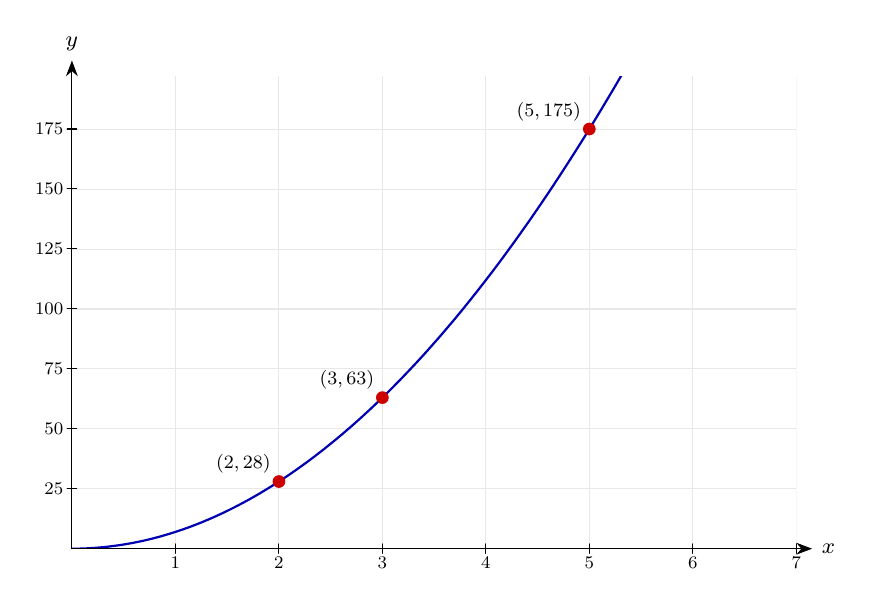
\begin{tikzpicture}[>={Stealth[length=2mm]},font=\footnotesize,line cap=round,line join=round]
\begin{scope}
\clip (0,0) rectangle (9.2,6);
\draw[gray!18] (0,0) grid[xstep=1.314,ystep=0.761] (9.2,6);
\draw[blue!70!black,thick] (0,0) -- (0.046,0) -- (0.092,0.001) -- (0.138,0.002) -- (0.184,0.004) -- (0.23,0.007) -- (0.276,0.009) -- (0.322,0.013) -- (0.368,0.017) -- (0.414,0.021) -- (0.46,0.026) -- (0.506,0.032) -- (0.552,0.038) -- (0.598,0.044) -- (0.644,0.051) -- (0.69,0.059) -- (0.736,0.067) -- (0.782,0.075) -- (0.828,0.085) -- (0.874,0.094) -- (0.92,0.104) -- (0.966,0.115) -- (1.012,0.126) -- (1.058,0.138) -- (1.104,0.15) -- (1.15,0.163) -- (1.196,0.177) -- (1.242,0.19) -- (1.288,0.205) -- (1.334,0.22) -- (1.38,0.235) -- (1.426,0.251) -- (1.472,0.267) -- (1.518,0.284) -- (1.564,0.302) -- (1.61,0.32) -- (1.656,0.338) -- (1.702,0.358) -- (1.748,0.377) -- (1.794,0.397) -- (1.84,0.418) -- (1.886,0.439) -- (1.932,0.461) -- (1.978,0.483) -- (2.024,0.506) -- (2.07,0.529) -- (2.116,0.553) -- (2.162,0.577) -- (2.208,0.602) -- (2.254,0.627) -- (2.3,0.653) -- (2.346,0.679) -- (2.392,0.706) -- (2.438,0.734) -- (2.484,0.762) -- (2.53,0.79) -- (2.576,0.819) -- (2.622,0.849) -- (2.668,0.879) -- (2.714,0.909) -- (2.76,0.94) -- (2.806,0.972) -- (2.852,1.004) -- (2.898,1.037) -- (2.944,1.07) -- (2.99,1.103) -- (3.036,1.138) -- (3.082,1.172) -- (3.128,1.208) -- (3.174,1.243) -- (3.22,1.28) -- (3.266,1.317) -- (3.312,1.354) -- (3.358,1.392) -- (3.404,1.43) -- (3.45,1.469) -- (3.496,1.509) -- (3.542,1.548) -- (3.588,1.589) -- (3.634,1.63) -- (3.68,1.671) -- (3.726,1.714) -- (3.772,1.756) -- (3.818,1.799) -- (3.864,1.843) -- (3.91,1.887) -- (3.956,1.932) -- (4.002,1.977) -- (4.048,2.022) -- (4.094,2.069) -- (4.14,2.115) -- (4.186,2.163) -- (4.232,2.211) -- (4.278,2.259) -- (4.324,2.308) -- (4.37,2.357) -- (4.416,2.407) -- (4.462,2.457) -- (4.508,2.508) -- (4.554,2.56) -- (4.6,2.612) -- (4.646,2.664) -- (4.692,2.717) -- (4.738,2.771) -- (4.784,2.825) -- (4.83,2.879) -- (4.876,2.934) -- (4.922,2.99) -- (4.968,3.046) -- (5.014,3.103) -- (5.06,3.16) -- (5.106,3.218) -- (5.152,3.276) -- (5.198,3.335) -- (5.244,3.394) -- (5.29,3.454) -- (5.336,3.514) -- (5.382,3.575) -- (5.428,3.636) -- (5.474,3.698) -- (5.52,3.761) -- (5.566,3.824) -- (5.612,3.887) -- (5.658,3.951) -- (5.704,4.016) -- (5.75,4.081) -- (5.796,4.146) -- (5.842,4.212) -- (5.888,4.279) -- (5.934,4.346) -- (5.98,4.414) -- (6.026,4.482) -- (6.072,4.551) -- (6.118,4.62) -- (6.164,4.69) -- (6.21,4.76) -- (6.256,4.831) -- (6.302,4.902) -- (6.348,4.974) -- (6.394,5.046) -- (6.44,5.119) -- (6.486,5.192) -- (6.532,5.266) -- (6.578,5.341) -- (6.624,5.416) -- (6.67,5.491) -- (6.716,5.567) -- (6.762,5.644) -- (6.808,5.721) -- (6.854,5.798) -- (6.9,5.876) -- (6.946,5.955) -- (6.992,6.034) -- (7.038,6.114) -- (7.084,6.194) -- (7.13,6.275) -- (7.176,6.356) -- (7.222,6.438) -- (7.268,6.52) -- (7.314,6.603) -- (7.36,6.686) -- (7.406,6.77) -- (7.452,6.854) -- (7.498,6.939) -- (7.544,7.024) -- (7.59,7.11) -- (7.636,7.197) -- (7.682,7.284) -- (7.728,7.371) -- (7.774,7.459) -- (7.82,7.548) -- (7.866,7.637) -- (7.912,7.726) -- (7.958,7.816) -- (8.004,7.907) -- (8.05,7.998) -- (8.096,8.09) -- (8.142,8.182) -- (8.188,8.275) -- (8.234,8.368) -- (8.28,8.462) -- (8.326,8.556) -- (8.372,8.651) -- (8.418,8.746) -- (8.464,8.842) -- (8.51,8.938) -- (8.556,9.035) -- (8.602,9.133) -- (8.648,9.231) -- (8.694,9.329) -- (8.74,9.428) -- (8.786,9.528) -- (8.832,9.628) -- (8.878,9.728) -- (8.924,9.829) -- (8.97,9.931) -- (9.016,10.033) -- (9.062,10.136) -- (9.108,10.239) -- (9.154,10.342) -- (9.2,10.447);
\end{scope}
\draw[->] (0,0) -- (9.4,0) node[right]{$x$};
\draw[->] (0,0) -- (0,6.2) node[above]{$y$};
\draw (1.314,-0.06) -- (1.314,0.06) node[below=2pt,scale=0.8]{$1$};
\draw (2.629,-0.06) -- (2.629,0.06) node[below=2pt,scale=0.8]{$2$};
\draw (3.943,-0.06) -- (3.943,0.06) node[below=2pt,scale=0.8]{$3$};
\draw (5.257,-0.06) -- (5.257,0.06) node[below=2pt,scale=0.8]{$4$};
\draw (6.571,-0.06) -- (6.571,0.06) node[below=2pt,scale=0.8]{$5$};
\draw (7.886,-0.06) -- (7.886,0.06) node[below=2pt,scale=0.8]{$6$};
\draw (9.2,-0.06) -- (9.2,0.06) node[below=2pt,scale=0.8]{$7$};
\draw (-0.06,0.761) -- (0.06,0.761) node[left=2pt,scale=0.8]{$25$};
\draw (-0.06,1.523) -- (0.06,1.523) node[left=2pt,scale=0.8]{$50$};
\draw (-0.06,2.284) -- (0.06,2.284) node[left=2pt,scale=0.8]{$75$};
\draw (-0.06,3.046) -- (0.06,3.046) node[left=2pt,scale=0.8]{$100$};
\draw (-0.06,3.807) -- (0.06,3.807) node[left=2pt,scale=0.8]{$125$};
\draw (-0.06,4.569) -- (0.06,4.569) node[left=2pt,scale=0.8]{$150$};
\draw (-0.06,5.33) -- (0.06,5.33) node[left=2pt,scale=0.8]{$175$};
\fill[red!80!black] (2.629,0.853) circle (2.3pt);
\node[above left,scale=0.85] at (2.629,0.853) {$(2,28)$};
\fill[red!80!black] (6.571,5.33) circle (2.3pt);
\node[above left,scale=0.85] at (6.571,5.33) {$(5,175)$};
\fill[red!80!black] (3.943,1.919) circle (2.3pt);
\node[above left,scale=0.85] at (3.943,1.919) {$(3,63)$};
\end{tikzpicture}
}
\end{center}
\small The relationship plotted, with the data points marked.\normalsize

\medskip\hrule

\section*{Proportion 34\quad\small\texttt{(cg4-034)}}
\addcontentsline{toc}{section}{Proportion 34 (cg4-034)}
\textit{Difficulty: Foundation \quad\textbar\quad Marks: 8}

\question{The variable \( P \) is inversely proportional to \( Q \). When \( Q = 5 \), \( P = 12 \). The variable \( R \) is directly proportional to \( Q^2 \). When \( Q = 2 \), \( R = 20 \). \\[3pt] a) Express \( P \) in terms of \( Q \). \\[3pt] b) Express \( R \) in terms of \( Q \). \\[3pt] c) Find the value of \( Q \) for which \( P = R \).}

\textbf{Worked solution.}

\textit{Step 1: Part a: find \( k_1 \) from \( P = \frac{k_1}{Q} \).}
\[\begin{gathered}
12 = \frac{k_1}{5} \implies k_1 = 60 \implies P = \frac{60}{Q}
\end{gathered}\]
Multiply both sides by 5.

\textit{Step 2: Part b: find \( k_2 \) from \( R = k_2 Q^2 \).}
\[\begin{gathered}
20 = k_2 \times 4 \implies k_2 = 5 \implies R = 5Q^2
\end{gathered}\]
Divide both sides by \( 2^2 = 4 \).

\textit{Step 3: Part c: set \( P = R \) and solve.}
\[\begin{gathered}
\frac{60}{Q} = 5Q^2 \implies 60 = 5Q^3 \implies Q^3 = 12
\end{gathered}\]
Multiply both sides by \( Q \) (assuming \( Q \neq 0 \)), then divide by 5.

\textit{Step 4: Find the exact value of \( Q \).}
\[\begin{gathered}
Q = \sqrt[3]{12}
\end{gathered}\]
Take the cube root of both sides. \( Q = \sqrt[3]{12} \approx 2.29 \).

\begin{answerbox}
\textbf{Final answer:}\quad a) \(\displaystyle P = \dfrac{60}{Q}\); b) \(\displaystyle R = 5Q^2\); c) \(\displaystyle Q = \sqrt[3]{12}\)
\end{answerbox}
\textbf{Graph.}

\begin{center}
\resizebox{\ifdim\width>\linewidth \linewidth\else \width\fi}{!}{%
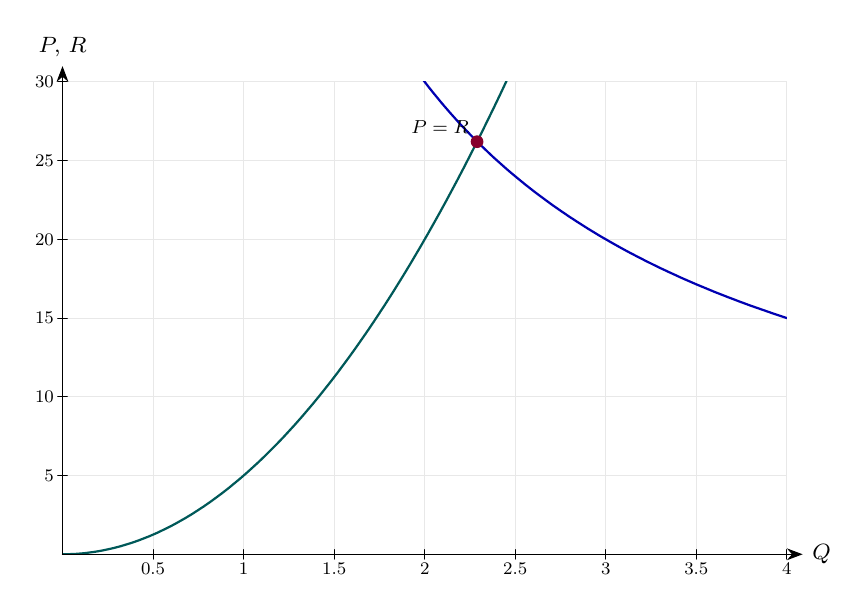
\begin{tikzpicture}[>={Stealth[length=2mm]},font=\footnotesize,line cap=round,line join=round]
\begin{scope}
\clip (0,0) rectangle (9.2,6);
\draw[gray!18] (0,0) grid[xstep=1.15,ystep=1] (9.2,6);
\draw[blue!70!black,thick] (0.023,12) -- (0.069,12) -- (0.115,12) -- (0.161,12) -- (0.207,12) -- (0.252,12) -- (0.298,12) -- (0.344,12) -- (0.39,12) -- (0.436,12) -- (0.482,12) -- (0.528,12) -- (0.574,12) -- (0.62,12) -- (0.665,12) -- (0.711,12) -- (0.757,12) -- (0.803,12) -- (0.849,12) -- (0.895,12) -- (0.941,12) -- (0.987,12) -- (1.032,12) -- (1.078,12) -- (1.124,12) -- (1.17,12) -- (1.216,12) -- (1.262,12) -- (1.308,12) -- (1.354,12) -- (1.4,12) -- (1.445,12) -- (1.491,12) -- (1.537,12) -- (1.583,12) -- (1.629,12) -- (1.675,12) -- (1.721,12) -- (1.767,12) -- (1.813,12) -- (1.858,12) -- (1.904,12) -- (1.95,12) -- (1.996,12) -- (2.042,12) -- (2.088,12) -- (2.134,12) -- (2.18,12) -- (2.225,12) -- (2.271,12) -- (2.317,11.911) -- (2.363,11.679) -- (2.409,11.457) -- (2.455,11.243) -- (2.501,11.037) -- (2.547,10.838) -- (2.593,10.646) -- (2.638,10.461) -- (2.684,10.282) -- (2.73,10.109) -- (2.776,9.942) -- (2.822,9.78) -- (2.868,9.624) -- (2.914,9.472) -- (2.96,9.325) -- (3.006,9.183) -- (3.051,9.045) -- (3.097,8.911) -- (3.143,8.781) -- (3.189,8.655) -- (3.235,8.532) -- (3.281,8.412) -- (3.327,8.296) -- (3.373,8.184) -- (3.418,8.074) -- (3.464,7.967) -- (3.51,7.863) -- (3.556,7.761) -- (3.602,7.662) -- (3.648,7.566) -- (3.694,7.472) -- (3.74,7.38) -- (3.786,7.291) -- (3.831,7.204) -- (3.877,7.118) -- (3.923,7.035) -- (3.969,6.954) -- (4.015,6.874) -- (4.061,6.797) -- (4.107,6.721) -- (4.153,6.646) -- (4.199,6.574) -- (4.244,6.503) -- (4.29,6.433) -- (4.336,6.365) -- (4.382,6.298) -- (4.428,6.233) -- (4.474,6.169) -- (4.52,6.107) -- (4.566,6.045) -- (4.611,5.985) -- (4.657,5.926) -- (4.703,5.868) -- (4.749,5.812) -- (4.795,5.756) -- (4.841,5.701) -- (4.887,5.648) -- (4.933,5.595) -- (4.979,5.544) -- (5.024,5.493) -- (5.07,5.443) -- (5.116,5.395) -- (5.162,5.347) -- (5.208,5.3) -- (5.254,5.253) -- (5.3,5.208) -- (5.346,5.163) -- (5.392,5.119) -- (5.437,5.076) -- (5.483,5.033) -- (5.529,4.992) -- (5.575,4.951) -- (5.621,4.91) -- (5.667,4.87) -- (5.713,4.831) -- (5.759,4.793) -- (5.805,4.755) -- (5.85,4.718) -- (5.896,4.681) -- (5.942,4.645) -- (5.988,4.609) -- (6.034,4.574) -- (6.08,4.54) -- (6.126,4.506) -- (6.172,4.472) -- (6.217,4.439) -- (6.263,4.407) -- (6.309,4.375) -- (6.355,4.343) -- (6.401,4.312) -- (6.447,4.281) -- (6.493,4.251) -- (6.539,4.221) -- (6.585,4.192) -- (6.63,4.163) -- (6.676,4.134) -- (6.722,4.106) -- (6.768,4.078) -- (6.814,4.05) -- (6.86,4.023) -- (6.906,3.997) -- (6.952,3.97) -- (6.998,3.944) -- (7.043,3.919) -- (7.089,3.893) -- (7.135,3.868) -- (7.181,3.843) -- (7.227,3.819) -- (7.273,3.795) -- (7.319,3.771) -- (7.365,3.748) -- (7.41,3.724) -- (7.456,3.702) -- (7.502,3.679) -- (7.548,3.657) -- (7.594,3.634) -- (7.64,3.613) -- (7.686,3.591) -- (7.732,3.57) -- (7.778,3.549) -- (7.823,3.528) -- (7.869,3.507) -- (7.915,3.487) -- (7.961,3.467) -- (8.007,3.447) -- (8.053,3.427) -- (8.099,3.408) -- (8.145,3.389) -- (8.191,3.37) -- (8.236,3.351) -- (8.282,3.332) -- (8.328,3.314) -- (8.374,3.296) -- (8.42,3.278) -- (8.466,3.26) -- (8.512,3.243) -- (8.558,3.225) -- (8.603,3.208) -- (8.649,3.191) -- (8.695,3.174) -- (8.741,3.157) -- (8.787,3.141) -- (8.833,3.125) -- (8.879,3.109) -- (8.925,3.093) -- (8.971,3.077) -- (9.016,3.061) -- (9.062,3.046) -- (9.108,3.03) -- (9.154,3.015) -- (9.2,3);
\draw[teal!70!black,thick] (0,0) -- (0.046,0) -- (0.092,0.002) -- (0.138,0.004) -- (0.184,0.006) -- (0.23,0.01) -- (0.276,0.014) -- (0.322,0.02) -- (0.368,0.026) -- (0.414,0.032) -- (0.46,0.04) -- (0.506,0.048) -- (0.552,0.058) -- (0.598,0.068) -- (0.644,0.078) -- (0.69,0.09) -- (0.736,0.102) -- (0.782,0.116) -- (0.828,0.13) -- (0.874,0.144) -- (0.92,0.16) -- (0.966,0.176) -- (1.012,0.194) -- (1.058,0.212) -- (1.104,0.23) -- (1.15,0.25) -- (1.196,0.27) -- (1.242,0.292) -- (1.288,0.314) -- (1.334,0.336) -- (1.38,0.36) -- (1.426,0.384) -- (1.472,0.41) -- (1.518,0.436) -- (1.564,0.462) -- (1.61,0.49) -- (1.656,0.518) -- (1.702,0.548) -- (1.748,0.578) -- (1.794,0.608) -- (1.84,0.64) -- (1.886,0.672) -- (1.932,0.706) -- (1.978,0.74) -- (2.024,0.774) -- (2.07,0.81) -- (2.116,0.846) -- (2.162,0.884) -- (2.208,0.922) -- (2.254,0.96) -- (2.3,1) -- (2.346,1.04) -- (2.392,1.082) -- (2.438,1.124) -- (2.484,1.166) -- (2.53,1.21) -- (2.576,1.254) -- (2.622,1.3) -- (2.668,1.346) -- (2.714,1.392) -- (2.76,1.44) -- (2.806,1.488) -- (2.852,1.538) -- (2.898,1.588) -- (2.944,1.638) -- (2.99,1.69) -- (3.036,1.742) -- (3.082,1.796) -- (3.128,1.85) -- (3.174,1.904) -- (3.22,1.96) -- (3.266,2.016) -- (3.312,2.074) -- (3.358,2.132) -- (3.404,2.19) -- (3.45,2.25) -- (3.496,2.31) -- (3.542,2.372) -- (3.588,2.434) -- (3.634,2.496) -- (3.68,2.56) -- (3.726,2.624) -- (3.772,2.69) -- (3.818,2.756) -- (3.864,2.822) -- (3.91,2.89) -- (3.956,2.958) -- (4.002,3.028) -- (4.048,3.098) -- (4.094,3.168) -- (4.14,3.24) -- (4.186,3.312) -- (4.232,3.386) -- (4.278,3.46) -- (4.324,3.534) -- (4.37,3.61) -- (4.416,3.686) -- (4.462,3.764) -- (4.508,3.842) -- (4.554,3.92) -- (4.6,4) -- (4.646,4.08) -- (4.692,4.162) -- (4.738,4.244) -- (4.784,4.326) -- (4.83,4.41) -- (4.876,4.494) -- (4.922,4.58) -- (4.968,4.666) -- (5.014,4.752) -- (5.06,4.84) -- (5.106,4.928) -- (5.152,5.018) -- (5.198,5.108) -- (5.244,5.198) -- (5.29,5.29) -- (5.336,5.382) -- (5.382,5.476) -- (5.428,5.57) -- (5.474,5.664) -- (5.52,5.76) -- (5.566,5.856) -- (5.612,5.954) -- (5.658,6.052) -- (5.704,6.15) -- (5.75,6.25) -- (5.796,6.35) -- (5.842,6.452) -- (5.888,6.554) -- (5.934,6.656) -- (5.98,6.76) -- (6.026,6.864) -- (6.072,6.97) -- (6.118,7.076) -- (6.164,7.182) -- (6.21,7.29) -- (6.256,7.398) -- (6.302,7.508) -- (6.348,7.618) -- (6.394,7.728) -- (6.44,7.84) -- (6.486,7.952) -- (6.532,8.066) -- (6.578,8.18) -- (6.624,8.294) -- (6.67,8.41) -- (6.716,8.526) -- (6.762,8.644) -- (6.808,8.762) -- (6.854,8.88) -- (6.9,9) -- (6.946,9.12) -- (6.992,9.242) -- (7.038,9.364) -- (7.084,9.486) -- (7.13,9.61) -- (7.176,9.734) -- (7.222,9.86) -- (7.268,9.986) -- (7.314,10.112) -- (7.36,10.24) -- (7.406,10.368) -- (7.452,10.498) -- (7.498,10.628) -- (7.544,10.758) -- (7.59,10.89) -- (7.636,11.022) -- (7.682,11.156) -- (7.728,11.29) -- (7.774,11.424) -- (7.82,11.56) -- (7.866,11.696) -- (7.912,11.834) -- (7.958,11.972) -- (8.004,12) -- (8.05,12) -- (8.096,12) -- (8.142,12) -- (8.188,12) -- (8.234,12) -- (8.28,12) -- (8.326,12) -- (8.372,12) -- (8.418,12) -- (8.464,12) -- (8.51,12) -- (8.556,12) -- (8.602,12) -- (8.648,12) -- (8.694,12) -- (8.74,12) -- (8.786,12) -- (8.832,12) -- (8.878,12) -- (8.924,12) -- (8.97,12) -- (9.016,12) -- (9.062,12) -- (9.108,12) -- (9.154,12) -- (9.2,12);
\end{scope}
\draw[->] (0,0) -- (9.4,0) node[right]{$Q$};
\draw[->] (0,0) -- (0,6.2) node[above]{$P,\,R$};
\draw (1.15,-0.06) -- (1.15,0.06) node[below=2pt,scale=0.8]{$0.5$};
\draw (2.3,-0.06) -- (2.3,0.06) node[below=2pt,scale=0.8]{$1$};
\draw (3.45,-0.06) -- (3.45,0.06) node[below=2pt,scale=0.8]{$1.5$};
\draw (4.6,-0.06) -- (4.6,0.06) node[below=2pt,scale=0.8]{$2$};
\draw (5.75,-0.06) -- (5.75,0.06) node[below=2pt,scale=0.8]{$2.5$};
\draw (6.9,-0.06) -- (6.9,0.06) node[below=2pt,scale=0.8]{$3$};
\draw (8.05,-0.06) -- (8.05,0.06) node[below=2pt,scale=0.8]{$3.5$};
\draw (9.2,-0.06) -- (9.2,0.06) node[below=2pt,scale=0.8]{$4$};
\draw (-0.06,1) -- (0.06,1) node[left=2pt,scale=0.8]{$5$};
\draw (-0.06,2) -- (0.06,2) node[left=2pt,scale=0.8]{$10$};
\draw (-0.06,3) -- (0.06,3) node[left=2pt,scale=0.8]{$15$};
\draw (-0.06,4) -- (0.06,4) node[left=2pt,scale=0.8]{$20$};
\draw (-0.06,5) -- (0.06,5) node[left=2pt,scale=0.8]{$25$};
\draw (-0.06,6) -- (0.06,6) node[left=2pt,scale=0.8]{$30$};
\fill[purple!70!black] (5.265,5.24) circle (2.3pt);
\node[above left,scale=0.85] at (5.265,5.24) {$P=R$};
\end{tikzpicture}
}
\end{center}
\small The relationship plotted, with the data points marked.\normalsize

\medskip\hrule

\section*{Proportion 35\quad\small\texttt{(cg4-035)}}
\addcontentsline{toc}{section}{Proportion 35 (cg4-035)}
\textit{Difficulty: Foundation \quad\textbar\quad Marks: 10}

\question{The variable \( y \) is inversely proportional to the square of \( x \). When \( x = 2 \), \( y = 50 \). \\[3pt] a) Find the value of \( y \) when \( x = 10 \). \\[3pt] b) Find the exact values of \( x \) when \( y = 8 \). \\[3pt] c) Show that when \( x \) is halved, \( y \) increases by a factor of 4. \\[3pt] d) Given that \( z \propto y \) and \( z = 30 \) when \( y = 50 \), find \( z \) when \( x = 5 \).}

\textbf{Worked solution.}

\textit{Step 1: Find \( k \): write \( y = \frac{k}{x^2} \).}
\[\begin{gathered}
50 = \frac{k}{4} \implies k = 200
\end{gathered}\]
Multiply both sides by \( 2^2 = 4 \).

\textit{Step 2: Part a: substitute \( x = 10 \).}
\[\begin{gathered}
y = \frac{200}{100} = 2
\end{gathered}\]
\( 10^2 = 100 \).

\textit{Step 3: Part b: substitute \( y = 8 \) and solve.}
\[\begin{gathered}
8 = \frac{200}{x^2} \implies x^2 = 25 \implies x = \pm 5
\end{gathered}\]
Divide 200 by 8 to get \( x^2 = 25 \), then take square roots.

\textit{Step 4: Part c: replace \( x \) with \( \frac{x}{2} \).}
\[\begin{gathered}
y_{\text{new}} = \frac{200}{\left(\frac{x}{2}\right)^2} = \frac{200}{\frac{x^2}{4}} = \frac{800}{x^2} = 4 \times \frac{200}{x^2} = 4y
\end{gathered}\]
Halving \( x \) quarters \( x^2 \), which quadruples \( y \). \( \square \)

\textit{Step 5: Part d: find \( m \) from \( z = my \).}
\[\begin{gathered}
30 = m \times 50 \implies m = \frac{3}{5}
\end{gathered}\]
Divide both sides by 50.

\textit{Step 6: Find \( y \) when \( x = 5 \), then find \( z \).}
\[\begin{gathered}
y = \frac{200}{25} = 8 \implies z = \frac{3}{5} \times 8 = \frac{24}{5} = 4.8
\end{gathered}\]
\( 5^2 = 25 \); multiply by \( m \).

\begin{answerbox}
\textbf{Final answer:}\quad a) \(\displaystyle y = 2\); b) \(\displaystyle x = \pm 5\); c) shown; d) \(\displaystyle z = 4.8\)
\end{answerbox}
\textbf{Graph.}

\begin{center}
\resizebox{\ifdim\width>\linewidth \linewidth\else \width\fi}{!}{%
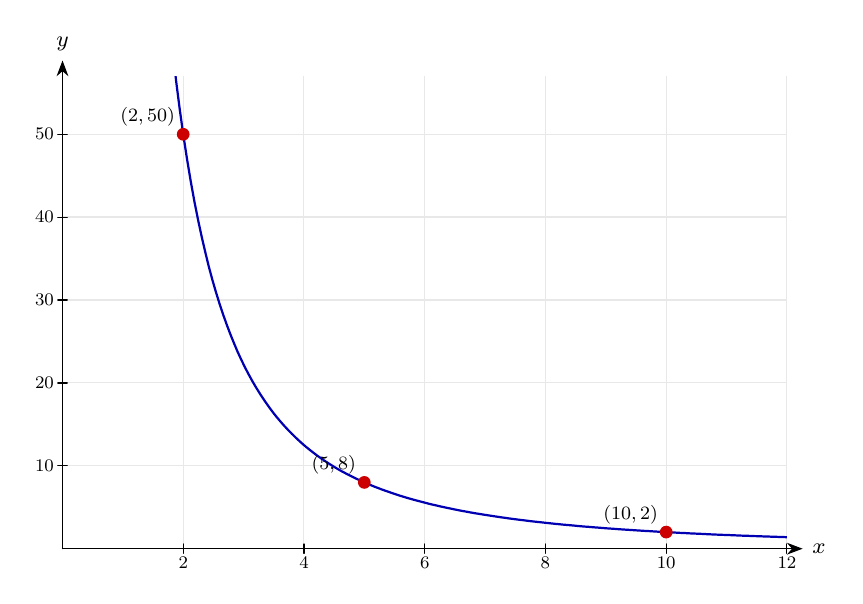
\begin{tikzpicture}[>={Stealth[length=2mm]},font=\footnotesize,line cap=round,line join=round]
\begin{scope}
\clip (0,0) rectangle (9.2,6);
\draw[gray!18] (0,0) grid[xstep=1.533,ystep=1.053] (9.2,6);
\draw[blue!70!black,thick] (0.023,12) -- (0.069,12) -- (0.115,12) -- (0.161,12) -- (0.207,12) -- (0.252,12) -- (0.298,12) -- (0.344,12) -- (0.39,12) -- (0.436,12) -- (0.482,12) -- (0.528,12) -- (0.574,12) -- (0.62,12) -- (0.665,12) -- (0.711,12) -- (0.757,12) -- (0.803,12) -- (0.849,12) -- (0.895,12) -- (0.941,12) -- (0.987,12) -- (1.032,11.608) -- (1.078,10.641) -- (1.124,9.79) -- (1.17,9.038) -- (1.216,8.368) -- (1.262,7.771) -- (1.308,7.235) -- (1.354,6.753) -- (1.4,6.317) -- (1.445,5.923) -- (1.491,5.564) -- (1.537,5.237) -- (1.583,4.938) -- (1.629,4.663) -- (1.675,4.411) -- (1.721,4.179) -- (1.767,3.965) -- (1.813,3.767) -- (1.858,3.583) -- (1.904,3.412) -- (1.95,3.254) -- (1.996,3.106) -- (2.042,2.968) -- (2.088,2.839) -- (2.134,2.718) -- (2.18,2.605) -- (2.225,2.498) -- (2.271,2.399) -- (2.317,2.304) -- (2.363,2.216) -- (2.409,2.132) -- (2.455,2.053) -- (2.501,1.979) -- (2.547,1.908) -- (2.593,1.841) -- (2.638,1.778) -- (2.684,1.717) -- (2.73,1.66) -- (2.776,1.606) -- (2.822,1.554) -- (2.868,1.505) -- (2.914,1.458) -- (2.96,1.413) -- (3.006,1.37) -- (3.051,1.329) -- (3.097,1.29) -- (3.143,1.253) -- (3.189,1.217) -- (3.235,1.182) -- (3.281,1.15) -- (3.327,1.118) -- (3.373,1.088) -- (3.418,1.059) -- (3.464,1.031) -- (3.51,1.004) -- (3.556,0.978) -- (3.602,0.954) -- (3.648,0.93) -- (3.694,0.907) -- (3.74,0.885) -- (3.786,0.863) -- (3.831,0.843) -- (3.877,0.823) -- (3.923,0.804) -- (3.969,0.785) -- (4.015,0.768) -- (4.061,0.75) -- (4.107,0.734) -- (4.153,0.718) -- (4.199,0.702) -- (4.244,0.687) -- (4.29,0.672) -- (4.336,0.658) -- (4.382,0.644) -- (4.428,0.631) -- (4.474,0.618) -- (4.52,0.606) -- (4.566,0.594) -- (4.612,0.582) -- (4.657,0.57) -- (4.703,0.559) -- (4.749,0.549) -- (4.795,0.538) -- (4.841,0.528) -- (4.887,0.518) -- (4.933,0.509) -- (4.979,0.499) -- (5.024,0.49) -- (5.07,0.481) -- (5.116,0.473) -- (5.162,0.464) -- (5.208,0.456) -- (5.254,0.448) -- (5.3,0.441) -- (5.346,0.433) -- (5.392,0.426) -- (5.437,0.419) -- (5.483,0.412) -- (5.529,0.405) -- (5.575,0.398) -- (5.621,0.392) -- (5.667,0.385) -- (5.713,0.379) -- (5.759,0.373) -- (5.805,0.367) -- (5.85,0.362) -- (5.896,0.356) -- (5.942,0.35) -- (5.988,0.345) -- (6.034,0.34) -- (6.08,0.335) -- (6.126,0.33) -- (6.172,0.325) -- (6.217,0.32) -- (6.263,0.315) -- (6.309,0.311) -- (6.355,0.306) -- (6.401,0.302) -- (6.447,0.298) -- (6.493,0.294) -- (6.539,0.289) -- (6.585,0.285) -- (6.63,0.281) -- (6.676,0.278) -- (6.722,0.274) -- (6.768,0.27) -- (6.814,0.267) -- (6.86,0.263) -- (6.906,0.259) -- (6.952,0.256) -- (6.998,0.253) -- (7.043,0.249) -- (7.089,0.246) -- (7.135,0.243) -- (7.181,0.24) -- (7.227,0.237) -- (7.273,0.234) -- (7.319,0.231) -- (7.365,0.228) -- (7.41,0.225) -- (7.456,0.223) -- (7.502,0.22) -- (7.548,0.217) -- (7.594,0.215) -- (7.64,0.212) -- (7.686,0.209) -- (7.732,0.207) -- (7.778,0.205) -- (7.823,0.202) -- (7.869,0.2) -- (7.915,0.198) -- (7.961,0.195) -- (8.007,0.193) -- (8.053,0.191) -- (8.099,0.189) -- (8.145,0.187) -- (8.191,0.184) -- (8.236,0.182) -- (8.282,0.18) -- (8.328,0.178) -- (8.374,0.176) -- (8.42,0.175) -- (8.466,0.173) -- (8.512,0.171) -- (8.558,0.169) -- (8.603,0.167) -- (8.649,0.165) -- (8.695,0.164) -- (8.741,0.162) -- (8.787,0.16) -- (8.833,0.159) -- (8.879,0.157) -- (8.925,0.155) -- (8.971,0.154) -- (9.016,0.152) -- (9.062,0.151) -- (9.108,0.149) -- (9.154,0.148) -- (9.2,0.146);
\end{scope}
\draw[->] (0,0) -- (9.4,0) node[right]{$x$};
\draw[->] (0,0) -- (0,6.2) node[above]{$y$};
\draw (1.533,-0.06) -- (1.533,0.06) node[below=2pt,scale=0.8]{$2$};
\draw (3.067,-0.06) -- (3.067,0.06) node[below=2pt,scale=0.8]{$4$};
\draw (4.6,-0.06) -- (4.6,0.06) node[below=2pt,scale=0.8]{$6$};
\draw (6.133,-0.06) -- (6.133,0.06) node[below=2pt,scale=0.8]{$8$};
\draw (7.667,-0.06) -- (7.667,0.06) node[below=2pt,scale=0.8]{$10$};
\draw (9.2,-0.06) -- (9.2,0.06) node[below=2pt,scale=0.8]{$12$};
\draw (-0.06,1.053) -- (0.06,1.053) node[left=2pt,scale=0.8]{$10$};
\draw (-0.06,2.105) -- (0.06,2.105) node[left=2pt,scale=0.8]{$20$};
\draw (-0.06,3.158) -- (0.06,3.158) node[left=2pt,scale=0.8]{$30$};
\draw (-0.06,4.211) -- (0.06,4.211) node[left=2pt,scale=0.8]{$40$};
\draw (-0.06,5.263) -- (0.06,5.263) node[left=2pt,scale=0.8]{$50$};
\fill[red!80!black] (1.533,5.263) circle (2.3pt);
\node[above left,scale=0.85] at (1.533,5.263) {$(2,50)$};
\fill[red!80!black] (3.833,0.842) circle (2.3pt);
\node[above left,scale=0.85] at (3.833,0.842) {$(5,8)$};
\fill[red!80!black] (7.667,0.211) circle (2.3pt);
\node[above left,scale=0.85] at (7.667,0.211) {$(10,2)$};
\end{tikzpicture}
}
\end{center}
\small The relationship plotted, with the data points marked.\normalsize

\medskip\hrule

\section*{Proportion 36\quad\small\texttt{(cg4-036)}}
\addcontentsline{toc}{section}{Proportion 36 (cg4-036)}
\textit{Difficulty: Foundation \quad\textbar\quad Marks: 3}

\question{Given that \( y \) is directly proportional to \( x \) and \( y = 15 \) when \( x = 5 \), find \( y \) when \( x = 8 \).}

\textbf{Worked solution.}

\textit{Step 1: Find k}
\[\begin{gathered}
y = kx \implies 15 = 5k \implies k = 3
\end{gathered}\]
\( y \propto x \) means \( y = kx \) for some constant \( k \). Substitute the given pair and divide both sides by 5 to isolate \( k \).

\textit{Step 2: Find y}
\[\begin{gathered}
y = 3 \times 8 = 24
\end{gathered}\]
Now that \( k \) is known, the equation \( y = 3x \) works for any \( x \); substitute the new value.

\begin{answerbox}
\textbf{Final answer:}\quad \(\displaystyle y = 24\)
\end{answerbox}
\textbf{Graph.}

\begin{center}
\resizebox{\ifdim\width>\linewidth \linewidth\else \width\fi}{!}{%
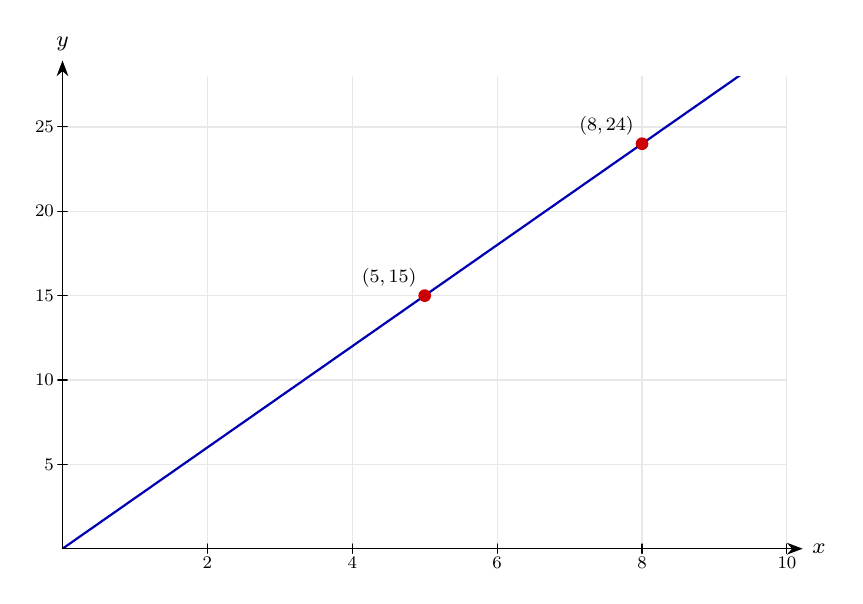
\begin{tikzpicture}[>={Stealth[length=2mm]},font=\footnotesize,line cap=round,line join=round]
\begin{scope}
\clip (0,0) rectangle (9.2,6);
\draw[gray!18] (0,0) grid[xstep=1.84,ystep=1.071] (9.2,6);
\draw[blue!70!black,thick] (0,0) -- (0.046,0.032) -- (0.092,0.064) -- (0.138,0.096) -- (0.184,0.129) -- (0.23,0.161) -- (0.276,0.193) -- (0.322,0.225) -- (0.368,0.257) -- (0.414,0.289) -- (0.46,0.321) -- (0.506,0.354) -- (0.552,0.386) -- (0.598,0.418) -- (0.644,0.45) -- (0.69,0.482) -- (0.736,0.514) -- (0.782,0.546) -- (0.828,0.579) -- (0.874,0.611) -- (0.92,0.643) -- (0.966,0.675) -- (1.012,0.707) -- (1.058,0.739) -- (1.104,0.771) -- (1.15,0.804) -- (1.196,0.836) -- (1.242,0.868) -- (1.288,0.9) -- (1.334,0.932) -- (1.38,0.964) -- (1.426,0.996) -- (1.472,1.029) -- (1.518,1.061) -- (1.564,1.093) -- (1.61,1.125) -- (1.656,1.157) -- (1.702,1.189) -- (1.748,1.221) -- (1.794,1.254) -- (1.84,1.286) -- (1.886,1.318) -- (1.932,1.35) -- (1.978,1.382) -- (2.024,1.414) -- (2.07,1.446) -- (2.116,1.479) -- (2.162,1.511) -- (2.208,1.543) -- (2.254,1.575) -- (2.3,1.607) -- (2.346,1.639) -- (2.392,1.671) -- (2.438,1.704) -- (2.484,1.736) -- (2.53,1.768) -- (2.576,1.8) -- (2.622,1.832) -- (2.668,1.864) -- (2.714,1.896) -- (2.76,1.929) -- (2.806,1.961) -- (2.852,1.993) -- (2.898,2.025) -- (2.944,2.057) -- (2.99,2.089) -- (3.036,2.121) -- (3.082,2.154) -- (3.128,2.186) -- (3.174,2.218) -- (3.22,2.25) -- (3.266,2.282) -- (3.312,2.314) -- (3.358,2.346) -- (3.404,2.379) -- (3.45,2.411) -- (3.496,2.443) -- (3.542,2.475) -- (3.588,2.507) -- (3.634,2.539) -- (3.68,2.571) -- (3.726,2.604) -- (3.772,2.636) -- (3.818,2.668) -- (3.864,2.7) -- (3.91,2.732) -- (3.956,2.764) -- (4.002,2.796) -- (4.048,2.829) -- (4.094,2.861) -- (4.14,2.893) -- (4.186,2.925) -- (4.232,2.957) -- (4.278,2.989) -- (4.324,3.021) -- (4.37,3.054) -- (4.416,3.086) -- (4.462,3.118) -- (4.508,3.15) -- (4.554,3.182) -- (4.6,3.214) -- (4.646,3.246) -- (4.692,3.279) -- (4.738,3.311) -- (4.784,3.343) -- (4.83,3.375) -- (4.876,3.407) -- (4.922,3.439) -- (4.968,3.471) -- (5.014,3.504) -- (5.06,3.536) -- (5.106,3.568) -- (5.152,3.6) -- (5.198,3.632) -- (5.244,3.664) -- (5.29,3.696) -- (5.336,3.729) -- (5.382,3.761) -- (5.428,3.793) -- (5.474,3.825) -- (5.52,3.857) -- (5.566,3.889) -- (5.612,3.921) -- (5.658,3.954) -- (5.704,3.986) -- (5.75,4.018) -- (5.796,4.05) -- (5.842,4.082) -- (5.888,4.114) -- (5.934,4.146) -- (5.98,4.179) -- (6.026,4.211) -- (6.072,4.243) -- (6.118,4.275) -- (6.164,4.307) -- (6.21,4.339) -- (6.256,4.371) -- (6.302,4.404) -- (6.348,4.436) -- (6.394,4.468) -- (6.44,4.5) -- (6.486,4.532) -- (6.532,4.564) -- (6.578,4.596) -- (6.624,4.629) -- (6.67,4.661) -- (6.716,4.693) -- (6.762,4.725) -- (6.808,4.757) -- (6.854,4.789) -- (6.9,4.821) -- (6.946,4.854) -- (6.992,4.886) -- (7.038,4.918) -- (7.084,4.95) -- (7.13,4.982) -- (7.176,5.014) -- (7.222,5.046) -- (7.268,5.079) -- (7.314,5.111) -- (7.36,5.143) -- (7.406,5.175) -- (7.452,5.207) -- (7.498,5.239) -- (7.544,5.271) -- (7.59,5.304) -- (7.636,5.336) -- (7.682,5.368) -- (7.728,5.4) -- (7.774,5.432) -- (7.82,5.464) -- (7.866,5.496) -- (7.912,5.529) -- (7.958,5.561) -- (8.004,5.593) -- (8.05,5.625) -- (8.096,5.657) -- (8.142,5.689) -- (8.188,5.721) -- (8.234,5.754) -- (8.28,5.786) -- (8.326,5.818) -- (8.372,5.85) -- (8.418,5.882) -- (8.464,5.914) -- (8.51,5.946) -- (8.556,5.979) -- (8.602,6.011) -- (8.648,6.043) -- (8.694,6.075) -- (8.74,6.107) -- (8.786,6.139) -- (8.832,6.171) -- (8.878,6.204) -- (8.924,6.236) -- (8.97,6.268) -- (9.016,6.3) -- (9.062,6.332) -- (9.108,6.364) -- (9.154,6.396) -- (9.2,6.429);
\end{scope}
\draw[->] (0,0) -- (9.4,0) node[right]{$x$};
\draw[->] (0,0) -- (0,6.2) node[above]{$y$};
\draw (1.84,-0.06) -- (1.84,0.06) node[below=2pt,scale=0.8]{$2$};
\draw (3.68,-0.06) -- (3.68,0.06) node[below=2pt,scale=0.8]{$4$};
\draw (5.52,-0.06) -- (5.52,0.06) node[below=2pt,scale=0.8]{$6$};
\draw (7.36,-0.06) -- (7.36,0.06) node[below=2pt,scale=0.8]{$8$};
\draw (9.2,-0.06) -- (9.2,0.06) node[below=2pt,scale=0.8]{$10$};
\draw (-0.06,1.071) -- (0.06,1.071) node[left=2pt,scale=0.8]{$5$};
\draw (-0.06,2.143) -- (0.06,2.143) node[left=2pt,scale=0.8]{$10$};
\draw (-0.06,3.214) -- (0.06,3.214) node[left=2pt,scale=0.8]{$15$};
\draw (-0.06,4.286) -- (0.06,4.286) node[left=2pt,scale=0.8]{$20$};
\draw (-0.06,5.357) -- (0.06,5.357) node[left=2pt,scale=0.8]{$25$};
\fill[red!80!black] (4.6,3.214) circle (2.3pt);
\node[above left,scale=0.85] at (4.6,3.214) {$(5,15)$};
\fill[red!80!black] (7.36,5.143) circle (2.3pt);
\node[above left,scale=0.85] at (7.36,5.143) {$(8,24)$};
\end{tikzpicture}
}
\end{center}
\small The relationship plotted, with the data points marked.\normalsize

\medskip\hrule

\section*{Proportion 37\quad\small\texttt{(cg4-037)}}
\addcontentsline{toc}{section}{Proportion 37 (cg4-037)}
\textit{Difficulty: Foundation \quad\textbar\quad Marks: 3}

\question{Given that \( y \) is inversely proportional to \( x \) and \( y = 6 \) when \( x = 4 \), find \( y \) when \( x = 12 \).}

\textbf{Worked solution.}

\textit{Step 1: Find k}
\[\begin{gathered}
y = \frac{k}{x} \implies 6 = \frac{k}{4} \implies k = 24
\end{gathered}\]
\( y \propto \frac{1}{x} \) translates to \( y = \frac{k}{x} \). Multiply both sides by 4 to clear the fraction and isolate \( k \).

\textit{Step 2: Find y}
\[\begin{gathered}
y = \frac{24}{12} = 2
\end{gathered}\]
Sense-check: tripling \( x \) (from 4 to 12) should cut \( y \) to one third (6 $\to$ 2), and it does.

\begin{answerbox}
\textbf{Final answer:}\quad \(\displaystyle y = 2\)
\end{answerbox}
\textbf{Graph.}

\begin{center}
\resizebox{\ifdim\width>\linewidth \linewidth\else \width\fi}{!}{%
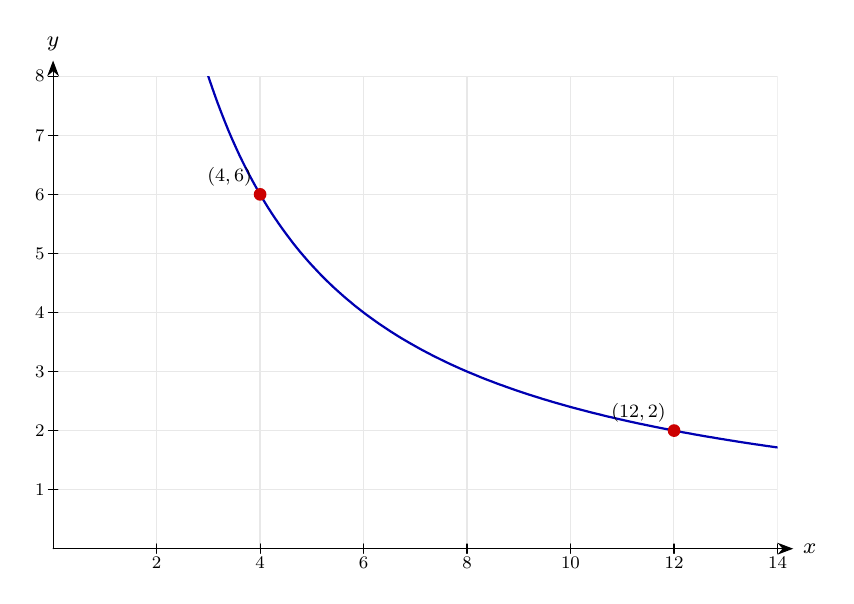
\begin{tikzpicture}[>={Stealth[length=2mm]},font=\footnotesize,line cap=round,line join=round]
\begin{scope}
\clip (0,0) rectangle (9.2,6);
\draw[gray!18] (0,0) grid[xstep=1.314,ystep=0.75] (9.2,6);
\draw[blue!70!black,thick] (0.023,12) -- (0.069,12) -- (0.115,12) -- (0.161,12) -- (0.207,12) -- (0.252,12) -- (0.298,12) -- (0.344,12) -- (0.39,12) -- (0.436,12) -- (0.482,12) -- (0.528,12) -- (0.574,12) -- (0.62,12) -- (0.665,12) -- (0.711,12) -- (0.757,12) -- (0.803,12) -- (0.849,12) -- (0.895,12) -- (0.941,12) -- (0.987,11.989) -- (1.032,11.457) -- (1.078,10.969) -- (1.124,10.521) -- (1.17,10.109) -- (1.216,9.727) -- (1.262,9.374) -- (1.308,9.045) -- (1.354,8.738) -- (1.4,8.452) -- (1.445,8.183) -- (1.491,7.932) -- (1.537,7.695) -- (1.583,7.472) -- (1.629,7.261) -- (1.675,7.062) -- (1.721,6.874) -- (1.767,6.696) -- (1.813,6.526) -- (1.858,6.365) -- (1.904,6.212) -- (1.95,6.065) -- (1.996,5.926) -- (2.042,5.793) -- (2.088,5.665) -- (2.134,5.544) -- (2.18,5.427) -- (2.225,5.315) -- (2.271,5.208) -- (2.317,5.105) -- (2.363,5.005) -- (2.409,4.91) -- (2.455,4.818) -- (2.501,4.73) -- (2.547,4.645) -- (2.593,4.563) -- (2.638,4.483) -- (2.684,4.407) -- (2.73,4.332) -- (2.776,4.261) -- (2.822,4.192) -- (2.868,4.125) -- (2.914,4.06) -- (2.96,3.997) -- (3.006,3.936) -- (3.051,3.876) -- (3.097,3.819) -- (3.143,3.763) -- (3.189,3.709) -- (3.235,3.656) -- (3.281,3.605) -- (3.327,3.556) -- (3.373,3.507) -- (3.418,3.46) -- (3.464,3.414) -- (3.51,3.37) -- (3.556,3.326) -- (3.602,3.284) -- (3.648,3.243) -- (3.694,3.202) -- (3.74,3.163) -- (3.786,3.125) -- (3.831,3.087) -- (3.877,3.051) -- (3.923,3.015) -- (3.969,2.98) -- (4.015,2.946) -- (4.061,2.913) -- (4.107,2.88) -- (4.153,2.848) -- (4.199,2.817) -- (4.244,2.787) -- (4.29,2.757) -- (4.336,2.728) -- (4.382,2.699) -- (4.428,2.671) -- (4.474,2.644) -- (4.52,2.617) -- (4.566,2.591) -- (4.612,2.565) -- (4.657,2.54) -- (4.703,2.515) -- (4.749,2.491) -- (4.795,2.467) -- (4.841,2.443) -- (4.887,2.421) -- (4.933,2.398) -- (4.979,2.376) -- (5.024,2.354) -- (5.07,2.333) -- (5.116,2.312) -- (5.162,2.291) -- (5.208,2.271) -- (5.254,2.251) -- (5.3,2.232) -- (5.346,2.213) -- (5.392,2.194) -- (5.437,2.175) -- (5.483,2.157) -- (5.529,2.139) -- (5.575,2.122) -- (5.621,2.104) -- (5.667,2.087) -- (5.713,2.071) -- (5.759,2.054) -- (5.805,2.038) -- (5.85,2.022) -- (5.896,2.006) -- (5.942,1.991) -- (5.988,1.975) -- (6.034,1.96) -- (6.08,1.946) -- (6.126,1.931) -- (6.172,1.917) -- (6.217,1.902) -- (6.263,1.889) -- (6.309,1.875) -- (6.355,1.861) -- (6.401,1.848) -- (6.447,1.835) -- (6.493,1.822) -- (6.539,1.809) -- (6.585,1.796) -- (6.63,1.784) -- (6.676,1.772) -- (6.722,1.76) -- (6.768,1.748) -- (6.814,1.736) -- (6.86,1.724) -- (6.906,1.713) -- (6.952,1.702) -- (6.998,1.69) -- (7.043,1.679) -- (7.089,1.669) -- (7.135,1.658) -- (7.181,1.647) -- (7.227,1.637) -- (7.273,1.626) -- (7.319,1.616) -- (7.365,1.606) -- (7.41,1.596) -- (7.456,1.586) -- (7.502,1.577) -- (7.548,1.567) -- (7.594,1.558) -- (7.64,1.548) -- (7.686,1.539) -- (7.732,1.53) -- (7.778,1.521) -- (7.823,1.512) -- (7.869,1.503) -- (7.915,1.494) -- (7.961,1.486) -- (8.007,1.477) -- (8.053,1.469) -- (8.099,1.461) -- (8.145,1.452) -- (8.191,1.444) -- (8.236,1.436) -- (8.282,1.428) -- (8.328,1.42) -- (8.374,1.413) -- (8.42,1.405) -- (8.466,1.397) -- (8.512,1.39) -- (8.558,1.382) -- (8.603,1.375) -- (8.649,1.368) -- (8.695,1.36) -- (8.741,1.353) -- (8.787,1.346) -- (8.833,1.339) -- (8.879,1.332) -- (8.925,1.325) -- (8.971,1.319) -- (9.016,1.312) -- (9.062,1.305) -- (9.108,1.299) -- (9.154,1.292) -- (9.2,1.286);
\end{scope}
\draw[->] (0,0) -- (9.4,0) node[right]{$x$};
\draw[->] (0,0) -- (0,6.2) node[above]{$y$};
\draw (1.314,-0.06) -- (1.314,0.06) node[below=2pt,scale=0.8]{$2$};
\draw (2.629,-0.06) -- (2.629,0.06) node[below=2pt,scale=0.8]{$4$};
\draw (3.943,-0.06) -- (3.943,0.06) node[below=2pt,scale=0.8]{$6$};
\draw (5.257,-0.06) -- (5.257,0.06) node[below=2pt,scale=0.8]{$8$};
\draw (6.571,-0.06) -- (6.571,0.06) node[below=2pt,scale=0.8]{$10$};
\draw (7.886,-0.06) -- (7.886,0.06) node[below=2pt,scale=0.8]{$12$};
\draw (9.2,-0.06) -- (9.2,0.06) node[below=2pt,scale=0.8]{$14$};
\draw (-0.06,0.75) -- (0.06,0.75) node[left=2pt,scale=0.8]{$1$};
\draw (-0.06,1.5) -- (0.06,1.5) node[left=2pt,scale=0.8]{$2$};
\draw (-0.06,2.25) -- (0.06,2.25) node[left=2pt,scale=0.8]{$3$};
\draw (-0.06,3) -- (0.06,3) node[left=2pt,scale=0.8]{$4$};
\draw (-0.06,3.75) -- (0.06,3.75) node[left=2pt,scale=0.8]{$5$};
\draw (-0.06,4.5) -- (0.06,4.5) node[left=2pt,scale=0.8]{$6$};
\draw (-0.06,5.25) -- (0.06,5.25) node[left=2pt,scale=0.8]{$7$};
\draw (-0.06,6) -- (0.06,6) node[left=2pt,scale=0.8]{$8$};
\fill[red!80!black] (2.629,4.5) circle (2.3pt);
\node[above left,scale=0.85] at (2.629,4.5) {$(4,6)$};
\fill[red!80!black] (7.886,1.5) circle (2.3pt);
\node[above left,scale=0.85] at (7.886,1.5) {$(12,2)$};
\end{tikzpicture}
}
\end{center}
\small The relationship plotted, with the data points marked.\normalsize

\medskip\hrule

\section*{Proportion 38\quad\small\texttt{(cg4-038)}}
\addcontentsline{toc}{section}{Proportion 38 (cg4-038)}
\textit{Difficulty: Foundation \quad\textbar\quad Marks: 3}

\question{\( y \) is proportional to \( x^2 \). When \( x = 3 \), \( y = 36 \). Find \( y \) when \( x = 5 \).}

\textbf{Worked solution.}

\textit{Step 1: Find k}
\[\begin{gathered}
y = kx^2 \implies 36 = 9k \implies k = 4
\end{gathered}\]
\( y \propto x^2 \) gives \( y = kx^2 \). Square \( x = 3 \) first to get 9, then divide. A common slip is to write \( 36 = 3k \) --- remember it is \( x^2 \), not \( x \).

\textit{Step 2: Find y}
\[\begin{gathered}
y = 4 \times 25 = 100
\end{gathered}\]
Square \( x = 5 \) first (giving 25), then multiply by \( k \). The order matters because \( kx^2 \neq (kx)^2 \).

\begin{answerbox}
\textbf{Final answer:}\quad \(\displaystyle y = 100\)
\end{answerbox}
\textbf{Graph.}

\begin{center}
\resizebox{\ifdim\width>\linewidth \linewidth\else \width\fi}{!}{%
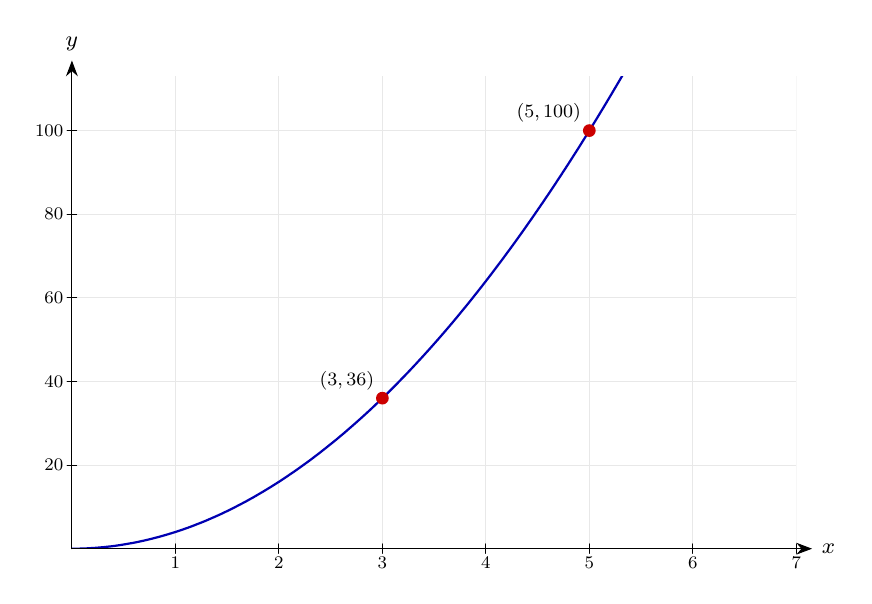
\begin{tikzpicture}[>={Stealth[length=2mm]},font=\footnotesize,line cap=round,line join=round]
\begin{scope}
\clip (0,0) rectangle (9.2,6);
\draw[gray!18] (0,0) grid[xstep=1.314,ystep=1.062] (9.2,6);
\draw[blue!70!black,thick] (0,0) -- (0.046,0) -- (0.092,0.001) -- (0.138,0.002) -- (0.184,0.004) -- (0.23,0.007) -- (0.276,0.009) -- (0.322,0.013) -- (0.368,0.017) -- (0.414,0.021) -- (0.46,0.026) -- (0.506,0.031) -- (0.552,0.037) -- (0.598,0.044) -- (0.644,0.051) -- (0.69,0.059) -- (0.736,0.067) -- (0.782,0.075) -- (0.828,0.084) -- (0.874,0.094) -- (0.92,0.104) -- (0.966,0.115) -- (1.012,0.126) -- (1.058,0.138) -- (1.104,0.15) -- (1.15,0.163) -- (1.196,0.176) -- (1.242,0.19) -- (1.288,0.204) -- (1.334,0.219) -- (1.38,0.234) -- (1.426,0.25) -- (1.472,0.266) -- (1.518,0.283) -- (1.564,0.301) -- (1.61,0.319) -- (1.656,0.337) -- (1.702,0.356) -- (1.748,0.376) -- (1.794,0.396) -- (1.84,0.416) -- (1.886,0.437) -- (1.932,0.459) -- (1.978,0.481) -- (2.024,0.504) -- (2.07,0.527) -- (2.116,0.551) -- (2.162,0.575) -- (2.208,0.599) -- (2.254,0.625) -- (2.3,0.65) -- (2.346,0.677) -- (2.392,0.704) -- (2.438,0.731) -- (2.484,0.759) -- (2.53,0.787) -- (2.576,0.816) -- (2.622,0.845) -- (2.668,0.875) -- (2.714,0.906) -- (2.76,0.937) -- (2.806,0.968) -- (2.852,1) -- (2.898,1.033) -- (2.944,1.066) -- (2.99,1.099) -- (3.036,1.133) -- (3.082,1.168) -- (3.128,1.203) -- (3.174,1.239) -- (3.22,1.275) -- (3.266,1.312) -- (3.312,1.349) -- (3.358,1.386) -- (3.404,1.425) -- (3.45,1.463) -- (3.496,1.503) -- (3.542,1.543) -- (3.588,1.583) -- (3.634,1.624) -- (3.68,1.665) -- (3.726,1.707) -- (3.772,1.749) -- (3.818,1.792) -- (3.864,1.836) -- (3.91,1.88) -- (3.956,1.924) -- (4.002,1.969) -- (4.048,2.015) -- (4.094,2.061) -- (4.14,2.107) -- (4.186,2.155) -- (4.232,2.202) -- (4.278,2.25) -- (4.324,2.299) -- (4.37,2.348) -- (4.416,2.398) -- (4.462,2.448) -- (4.508,2.499) -- (4.554,2.55) -- (4.6,2.602) -- (4.646,2.654) -- (4.692,2.707) -- (4.738,2.76) -- (4.784,2.814) -- (4.83,2.868) -- (4.876,2.923) -- (4.922,2.979) -- (4.968,3.035) -- (5.014,3.091) -- (5.06,3.148) -- (5.106,3.206) -- (5.152,3.264) -- (5.198,3.322) -- (5.244,3.381) -- (5.29,3.441) -- (5.336,3.501) -- (5.382,3.562) -- (5.428,3.623) -- (5.474,3.684) -- (5.52,3.747) -- (5.566,3.809) -- (5.612,3.872) -- (5.658,3.936) -- (5.704,4) -- (5.75,4.065) -- (5.796,4.131) -- (5.842,4.196) -- (5.888,4.263) -- (5.934,4.33) -- (5.98,4.397) -- (6.026,4.465) -- (6.072,4.533) -- (6.118,4.602) -- (6.164,4.672) -- (6.21,4.742) -- (6.256,4.812) -- (6.302,4.883) -- (6.348,4.955) -- (6.394,5.027) -- (6.44,5.099) -- (6.486,5.173) -- (6.532,5.246) -- (6.578,5.32) -- (6.624,5.395) -- (6.67,5.47) -- (6.716,5.546) -- (6.762,5.622) -- (6.808,5.699) -- (6.854,5.776) -- (6.9,5.854) -- (6.946,5.932) -- (6.992,6.011) -- (7.038,6.09) -- (7.084,6.17) -- (7.13,6.251) -- (7.176,6.332) -- (7.222,6.413) -- (7.268,6.495) -- (7.314,6.578) -- (7.36,6.661) -- (7.406,6.744) -- (7.452,6.828) -- (7.498,6.913) -- (7.544,6.998) -- (7.59,7.083) -- (7.636,7.169) -- (7.682,7.256) -- (7.728,7.343) -- (7.774,7.431) -- (7.82,7.519) -- (7.866,7.608) -- (7.912,7.697) -- (7.958,7.787) -- (8.004,7.877) -- (8.05,7.968) -- (8.096,8.059) -- (8.142,8.151) -- (8.188,8.243) -- (8.234,8.336) -- (8.28,8.43) -- (8.326,8.524) -- (8.372,8.618) -- (8.418,8.713) -- (8.464,8.809) -- (8.51,8.905) -- (8.556,9.001) -- (8.602,9.098) -- (8.648,9.196) -- (8.694,9.294) -- (8.74,9.392) -- (8.786,9.492) -- (8.832,9.591) -- (8.878,9.691) -- (8.924,9.792) -- (8.97,9.893) -- (9.016,9.995) -- (9.062,10.097) -- (9.108,10.2) -- (9.154,10.303) -- (9.2,10.407);
\end{scope}
\draw[->] (0,0) -- (9.4,0) node[right]{$x$};
\draw[->] (0,0) -- (0,6.2) node[above]{$y$};
\draw (1.314,-0.06) -- (1.314,0.06) node[below=2pt,scale=0.8]{$1$};
\draw (2.629,-0.06) -- (2.629,0.06) node[below=2pt,scale=0.8]{$2$};
\draw (3.943,-0.06) -- (3.943,0.06) node[below=2pt,scale=0.8]{$3$};
\draw (5.257,-0.06) -- (5.257,0.06) node[below=2pt,scale=0.8]{$4$};
\draw (6.571,-0.06) -- (6.571,0.06) node[below=2pt,scale=0.8]{$5$};
\draw (7.886,-0.06) -- (7.886,0.06) node[below=2pt,scale=0.8]{$6$};
\draw (9.2,-0.06) -- (9.2,0.06) node[below=2pt,scale=0.8]{$7$};
\draw (-0.06,1.062) -- (0.06,1.062) node[left=2pt,scale=0.8]{$20$};
\draw (-0.06,2.124) -- (0.06,2.124) node[left=2pt,scale=0.8]{$40$};
\draw (-0.06,3.186) -- (0.06,3.186) node[left=2pt,scale=0.8]{$60$};
\draw (-0.06,4.248) -- (0.06,4.248) node[left=2pt,scale=0.8]{$80$};
\draw (-0.06,5.31) -- (0.06,5.31) node[left=2pt,scale=0.8]{$100$};
\fill[red!80!black] (3.943,1.912) circle (2.3pt);
\node[above left,scale=0.85] at (3.943,1.912) {$(3,36)$};
\fill[red!80!black] (6.571,5.31) circle (2.3pt);
\node[above left,scale=0.85] at (6.571,5.31) {$(5,100)$};
\end{tikzpicture}
}
\end{center}
\small The relationship plotted, with the data points marked.\normalsize

\medskip\hrule

\section*{Proportion 39\quad\small\texttt{(cg4-039)}}
\addcontentsline{toc}{section}{Proportion 39 (cg4-039)}
\textit{Difficulty: Foundation \quad\textbar\quad Marks: 3}

\question{\( y \) is inversely proportional to \( \sqrt{x} \). When \( x = 9 \), \( y = 4 \). Find \( y \) when \( x = 16 \).}

\textbf{Worked solution.}

\textit{Step 1: Find k}
\[\begin{gathered}
y = \frac{k}{\sqrt{x}} \implies 4 = \frac{k}{3} \implies k = 12
\end{gathered}\]
\( y \propto \frac{1}{\sqrt{x}} \) means \( y = \frac{k}{\sqrt{x}} \). Evaluate \( \sqrt{9} = 3 \) first, then multiply both sides by 3.

\textit{Step 2: Find y}
\[\begin{gathered}
y = \frac{12}{\sqrt{16}} = \frac{12}{4} = 3
\end{gathered}\]
Take the square root before dividing --- \( \sqrt{16} = 4 \), not 16. Pitfall: students often forget the root and divide by \( x \) instead.

\begin{answerbox}
\textbf{Final answer:}\quad \(\displaystyle y = 3\)
\end{answerbox}
\textbf{Graph.}

\begin{center}
\resizebox{\ifdim\width>\linewidth \linewidth\else \width\fi}{!}{%
\begin{tikzpicture}[>={Stealth[length=2mm]},font=\footnotesize,line cap=round,line join=round]
\begin{scope}
\clip (0,0) rectangle (9.2,6);
\draw[gray!18] (0,0) grid[xstep=2.421,ystep=1.2] (9.2,6);
\draw[blue!70!black,thick] (0.023,12) -- (0.069,12) -- (0.115,12) -- (0.161,12) -- (0.207,12) -- (0.252,12) -- (0.298,12) -- (0.344,12) -- (0.39,12) -- (0.436,12) -- (0.482,12) -- (0.528,12) -- (0.574,12) -- (0.62,12) -- (0.665,12) -- (0.711,11.881) -- (0.757,11.516) -- (0.803,11.182) -- (0.849,10.875) -- (0.895,10.593) -- (0.941,10.331) -- (0.987,10.088) -- (1.032,9.861) -- (1.078,9.649) -- (1.124,9.45) -- (1.17,9.263) -- (1.216,9.087) -- (1.262,8.92) -- (1.308,8.762) -- (1.354,8.612) -- (1.4,8.47) -- (1.445,8.335) -- (1.491,8.205) -- (1.537,8.082) -- (1.583,7.964) -- (1.629,7.851) -- (1.675,7.743) -- (1.721,7.639) -- (1.767,7.539) -- (1.813,7.443) -- (1.858,7.35) -- (1.904,7.261) -- (1.95,7.175) -- (1.996,7.092) -- (2.042,7.012) -- (2.088,6.935) -- (2.134,6.86) -- (2.18,6.787) -- (2.225,6.717) -- (2.271,6.649) -- (2.317,6.583) -- (2.363,6.518) -- (2.409,6.456) -- (2.455,6.395) -- (2.501,6.336) -- (2.547,6.279) -- (2.593,6.223) -- (2.638,6.169) -- (2.684,6.116) -- (2.73,6.064) -- (2.776,6.014) -- (2.822,5.965) -- (2.868,5.917) -- (2.914,5.87) -- (2.96,5.825) -- (3.006,5.78) -- (3.051,5.736) -- (3.097,5.694) -- (3.143,5.652) -- (3.189,5.611) -- (3.235,5.571) -- (3.281,5.532) -- (3.327,5.494) -- (3.373,5.456) -- (3.418,5.42) -- (3.464,5.384) -- (3.51,5.348) -- (3.556,5.314) -- (3.602,5.28) -- (3.648,5.246) -- (3.694,5.214) -- (3.74,5.182) -- (3.786,5.15) -- (3.831,5.119) -- (3.877,5.089) -- (3.923,5.059) -- (3.969,5.03) -- (4.015,5.001) -- (4.061,4.972) -- (4.107,4.945) -- (4.153,4.917) -- (4.199,4.89) -- (4.244,4.864) -- (4.29,4.838) -- (4.336,4.812) -- (4.382,4.787) -- (4.428,4.762) -- (4.474,4.737) -- (4.52,4.713) -- (4.566,4.69) -- (4.611,4.666) -- (4.657,4.643) -- (4.703,4.62) -- (4.749,4.598) -- (4.795,4.576) -- (4.841,4.554) -- (4.887,4.533) -- (4.933,4.512) -- (4.979,4.491) -- (5.024,4.47) -- (5.07,4.45) -- (5.116,4.43) -- (5.162,4.41) -- (5.208,4.391) -- (5.254,4.372) -- (5.3,4.353) -- (5.346,4.334) -- (5.392,4.315) -- (5.437,4.297) -- (5.483,4.279) -- (5.529,4.261) -- (5.575,4.244) -- (5.621,4.226) -- (5.667,4.209) -- (5.713,4.192) -- (5.759,4.176) -- (5.805,4.159) -- (5.85,4.143) -- (5.896,4.127) -- (5.942,4.111) -- (5.988,4.095) -- (6.034,4.079) -- (6.08,4.064) -- (6.126,4.049) -- (6.172,4.033) -- (6.217,4.019) -- (6.263,4.004) -- (6.309,3.989) -- (6.355,3.975) -- (6.401,3.961) -- (6.447,3.946) -- (6.493,3.932) -- (6.539,3.919) -- (6.585,3.905) -- (6.63,3.891) -- (6.676,3.878) -- (6.722,3.865) -- (6.768,3.852) -- (6.814,3.839) -- (6.86,3.826) -- (6.906,3.813) -- (6.952,3.8) -- (6.998,3.788) -- (7.043,3.776) -- (7.089,3.763) -- (7.135,3.751) -- (7.181,3.739) -- (7.227,3.727) -- (7.273,3.716) -- (7.319,3.704) -- (7.365,3.692) -- (7.41,3.681) -- (7.456,3.67) -- (7.502,3.658) -- (7.548,3.647) -- (7.594,3.636) -- (7.64,3.625) -- (7.686,3.614) -- (7.732,3.604) -- (7.778,3.593) -- (7.823,3.582) -- (7.869,3.572) -- (7.915,3.562) -- (7.961,3.551) -- (8.007,3.541) -- (8.053,3.531) -- (8.099,3.521) -- (8.145,3.511) -- (8.191,3.501) -- (8.236,3.491) -- (8.282,3.482) -- (8.328,3.472) -- (8.374,3.463) -- (8.42,3.453) -- (8.466,3.444) -- (8.512,3.435) -- (8.558,3.425) -- (8.603,3.416) -- (8.649,3.407) -- (8.695,3.398) -- (8.741,3.389) -- (8.787,3.38) -- (8.833,3.372) -- (8.879,3.363) -- (8.925,3.354) -- (8.971,3.346) -- (9.016,3.337) -- (9.062,3.329) -- (9.108,3.32) -- (9.154,3.312) -- (9.2,3.304);
\end{scope}
\draw[->] (0,0) -- (9.4,0) node[right]{$x$};
\draw[->] (0,0) -- (0,6.2) node[above]{$y$};
\draw (2.421,-0.06) -- (2.421,0.06) node[below=2pt,scale=0.8]{$5$};
\draw (4.842,-0.06) -- (4.842,0.06) node[below=2pt,scale=0.8]{$10$};
\draw (7.263,-0.06) -- (7.263,0.06) node[below=2pt,scale=0.8]{$15$};
\draw (-0.06,1.2) -- (0.06,1.2) node[left=2pt,scale=0.8]{$1$};
\draw (-0.06,2.4) -- (0.06,2.4) node[left=2pt,scale=0.8]{$2$};
\draw (-0.06,3.6) -- (0.06,3.6) node[left=2pt,scale=0.8]{$3$};
\draw (-0.06,4.8) -- (0.06,4.8) node[left=2pt,scale=0.8]{$4$};
\draw (-0.06,6) -- (0.06,6) node[left=2pt,scale=0.8]{$5$};
\fill[red!80!black] (4.358,4.8) circle (2.3pt);
\node[above left,scale=0.85] at (4.358,4.8) {$(9,4)$};
\fill[red!80!black] (7.747,3.6) circle (2.3pt);
\node[above left,scale=0.85] at (7.747,3.6) {$(16,3)$};
\end{tikzpicture}
}
\end{center}
\small The relationship plotted, with the data points marked.\normalsize

\medskip\hrule

\section*{Proportion 40\quad\small\texttt{(cg4-040)}}
\addcontentsline{toc}{section}{Proportion 40 (cg4-040)}
\textit{Difficulty: Foundation \quad\textbar\quad Marks: 3}

\question{The cost \( C \) of fuel is directly proportional to the volume \( V \) litres bought. If 25 litres costs \( \pounds 37.50 \), find the cost of 40 litres.}

\textbf{Worked solution.}

\textit{Step 1: Find k}
\[\begin{gathered}
C = kV \implies 37.50 = 25k \implies k = 1.50
\end{gathered}\]
Direct proportion gives \( C = kV \). Here \( k \) is the price per litre --- divide total cost by litres to find it.

\textit{Step 2: Find C}
\[\begin{gathered}
C = 1.50 \times 40 = 60
\end{gathered}\]
Multiply the unit price by the new volume. Always sense-check: 40 litres is more than 25, so the cost should be more than \pounds 37.50.

\begin{answerbox}
\textbf{Final answer:}\quad \(\displaystyle \pounds 60\)
\end{answerbox}
\textbf{Graph.}

\begin{center}
\resizebox{\ifdim\width>\linewidth \linewidth\else \width\fi}{!}{%
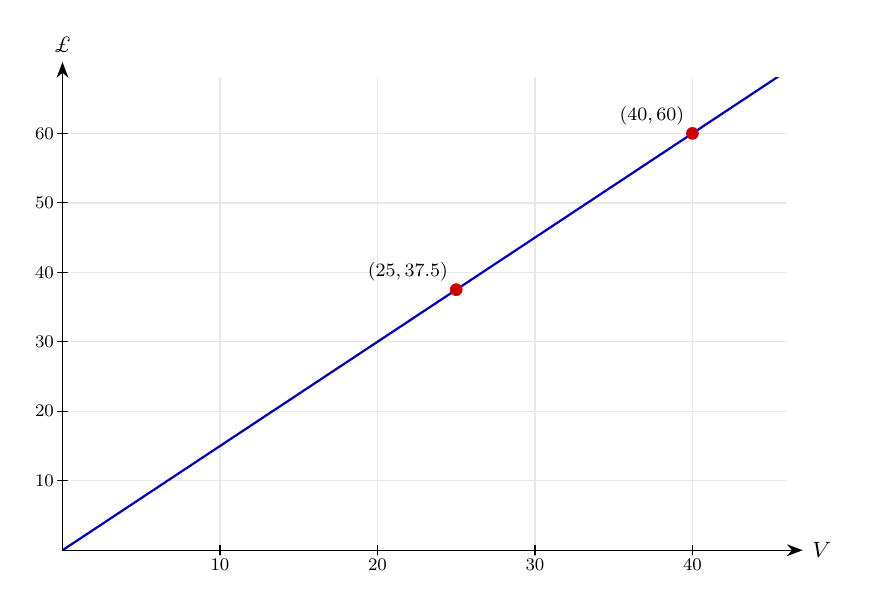
\begin{tikzpicture}[>={Stealth[length=2mm]},font=\footnotesize,line cap=round,line join=round]
\begin{scope}
\clip (0,0) rectangle (9.2,6);
\draw[gray!18] (0,0) grid[xstep=2,ystep=0.882] (9.2,6);
\draw[blue!70!black,thick] (0,0) -- (0.046,0.03) -- (0.092,0.061) -- (0.138,0.091) -- (0.184,0.122) -- (0.23,0.152) -- (0.276,0.183) -- (0.322,0.213) -- (0.368,0.244) -- (0.414,0.274) -- (0.46,0.304) -- (0.506,0.335) -- (0.552,0.365) -- (0.598,0.396) -- (0.644,0.426) -- (0.69,0.457) -- (0.736,0.487) -- (0.782,0.518) -- (0.828,0.548) -- (0.874,0.578) -- (0.92,0.609) -- (0.966,0.639) -- (1.012,0.67) -- (1.058,0.7) -- (1.104,0.731) -- (1.15,0.761) -- (1.196,0.791) -- (1.242,0.822) -- (1.288,0.852) -- (1.334,0.883) -- (1.38,0.913) -- (1.426,0.944) -- (1.472,0.974) -- (1.518,1.005) -- (1.564,1.035) -- (1.61,1.065) -- (1.656,1.096) -- (1.702,1.126) -- (1.748,1.157) -- (1.794,1.187) -- (1.84,1.218) -- (1.886,1.248) -- (1.932,1.279) -- (1.978,1.309) -- (2.024,1.339) -- (2.07,1.37) -- (2.116,1.4) -- (2.162,1.431) -- (2.208,1.461) -- (2.254,1.492) -- (2.3,1.522) -- (2.346,1.552) -- (2.392,1.583) -- (2.438,1.613) -- (2.484,1.644) -- (2.53,1.674) -- (2.576,1.705) -- (2.622,1.735) -- (2.668,1.766) -- (2.714,1.796) -- (2.76,1.826) -- (2.806,1.857) -- (2.852,1.887) -- (2.898,1.918) -- (2.944,1.948) -- (2.99,1.979) -- (3.036,2.009) -- (3.082,2.04) -- (3.128,2.07) -- (3.174,2.1) -- (3.22,2.131) -- (3.266,2.161) -- (3.312,2.192) -- (3.358,2.222) -- (3.404,2.253) -- (3.45,2.283) -- (3.496,2.314) -- (3.542,2.344) -- (3.588,2.374) -- (3.634,2.405) -- (3.68,2.435) -- (3.726,2.466) -- (3.772,2.496) -- (3.818,2.527) -- (3.864,2.557) -- (3.91,2.588) -- (3.956,2.618) -- (4.002,2.648) -- (4.048,2.679) -- (4.094,2.709) -- (4.14,2.74) -- (4.186,2.77) -- (4.232,2.801) -- (4.278,2.831) -- (4.324,2.861) -- (4.37,2.892) -- (4.416,2.922) -- (4.462,2.953) -- (4.508,2.983) -- (4.554,3.014) -- (4.6,3.044) -- (4.646,3.075) -- (4.692,3.105) -- (4.738,3.135) -- (4.784,3.166) -- (4.83,3.196) -- (4.876,3.227) -- (4.922,3.257) -- (4.968,3.288) -- (5.014,3.318) -- (5.06,3.349) -- (5.106,3.379) -- (5.152,3.409) -- (5.198,3.44) -- (5.244,3.47) -- (5.29,3.501) -- (5.336,3.531) -- (5.382,3.562) -- (5.428,3.592) -- (5.474,3.622) -- (5.52,3.653) -- (5.566,3.683) -- (5.612,3.714) -- (5.658,3.744) -- (5.704,3.775) -- (5.75,3.805) -- (5.796,3.836) -- (5.842,3.866) -- (5.888,3.896) -- (5.934,3.927) -- (5.98,3.957) -- (6.026,3.988) -- (6.072,4.018) -- (6.118,4.049) -- (6.164,4.079) -- (6.21,4.11) -- (6.256,4.14) -- (6.302,4.17) -- (6.348,4.201) -- (6.394,4.231) -- (6.44,4.262) -- (6.486,4.292) -- (6.532,4.323) -- (6.578,4.353) -- (6.624,4.384) -- (6.67,4.414) -- (6.716,4.444) -- (6.762,4.475) -- (6.808,4.505) -- (6.854,4.536) -- (6.9,4.566) -- (6.946,4.597) -- (6.992,4.627) -- (7.038,4.657) -- (7.084,4.688) -- (7.13,4.718) -- (7.176,4.749) -- (7.222,4.779) -- (7.268,4.81) -- (7.314,4.84) -- (7.36,4.871) -- (7.406,4.901) -- (7.452,4.931) -- (7.498,4.962) -- (7.544,4.992) -- (7.59,5.023) -- (7.636,5.053) -- (7.682,5.084) -- (7.728,5.114) -- (7.774,5.145) -- (7.82,5.175) -- (7.866,5.205) -- (7.912,5.236) -- (7.958,5.266) -- (8.004,5.297) -- (8.05,5.327) -- (8.096,5.358) -- (8.142,5.388) -- (8.188,5.419) -- (8.234,5.449) -- (8.28,5.479) -- (8.326,5.51) -- (8.372,5.54) -- (8.418,5.571) -- (8.464,5.601) -- (8.51,5.632) -- (8.556,5.662) -- (8.602,5.693) -- (8.648,5.723) -- (8.694,5.753) -- (8.74,5.784) -- (8.786,5.814) -- (8.832,5.845) -- (8.878,5.875) -- (8.924,5.906) -- (8.97,5.936) -- (9.016,5.966) -- (9.062,5.997) -- (9.108,6.027) -- (9.154,6.058) -- (9.2,6.088);
\end{scope}
\draw[->] (0,0) -- (9.4,0) node[right]{$V$};
\draw[->] (0,0) -- (0,6.2) node[above]{$\pounds$};
\draw (2,-0.06) -- (2,0.06) node[below=2pt,scale=0.8]{$10$};
\draw (4,-0.06) -- (4,0.06) node[below=2pt,scale=0.8]{$20$};
\draw (6,-0.06) -- (6,0.06) node[below=2pt,scale=0.8]{$30$};
\draw (8,-0.06) -- (8,0.06) node[below=2pt,scale=0.8]{$40$};
\draw (-0.06,0.882) -- (0.06,0.882) node[left=2pt,scale=0.8]{$10$};
\draw (-0.06,1.765) -- (0.06,1.765) node[left=2pt,scale=0.8]{$20$};
\draw (-0.06,2.647) -- (0.06,2.647) node[left=2pt,scale=0.8]{$30$};
\draw (-0.06,3.529) -- (0.06,3.529) node[left=2pt,scale=0.8]{$40$};
\draw (-0.06,4.412) -- (0.06,4.412) node[left=2pt,scale=0.8]{$50$};
\draw (-0.06,5.294) -- (0.06,5.294) node[left=2pt,scale=0.8]{$60$};
\fill[red!80!black] (5,3.309) circle (2.3pt);
\node[above left,scale=0.85] at (5,3.309) {$(25,37.5)$};
\fill[red!80!black] (8,5.294) circle (2.3pt);
\node[above left,scale=0.85] at (8,5.294) {$(40,60)$};
\end{tikzpicture}
}
\end{center}
\small The relationship plotted, with the data points marked.\normalsize

\medskip\hrule

\section*{Proportion 41\quad\small\texttt{(cg4-041)}}
\addcontentsline{toc}{section}{Proportion 41 (cg4-041)}
\textit{Difficulty: Foundation \quad\textbar\quad Marks: 4}

\question{\( y \) is proportional to \( x^3 \). When \( x = 2 \), \( y = 40 \). Find \( x \) when \( y = 135 \).}

\textbf{Worked solution.}

\textit{Step 1: Find k}
\[\begin{gathered}
y = kx^3 \implies 40 = 8k \implies k = 5
\end{gathered}\]
\( y \propto x^3 \) gives \( y = kx^3 \). Cube \( x = 2 \) to get 8 before dividing --- do not confuse \( x^3 \) with \( 3x \).

\textit{Step 2: Find x}
\[\begin{gathered}
135 = 5x^3 \implies x^3 = 27 \implies x = 3
\end{gathered}\]
Divide both sides by 5 to isolate \( x^3 \), then take the cube root. Unlike square roots, cube roots have a single real value, so no \( \pm \) is needed.

\begin{answerbox}
\textbf{Final answer:}\quad \(\displaystyle x = 3\)
\end{answerbox}
\textbf{Graph.}

\begin{center}
\resizebox{\ifdim\width>\linewidth \linewidth\else \width\fi}{!}{%
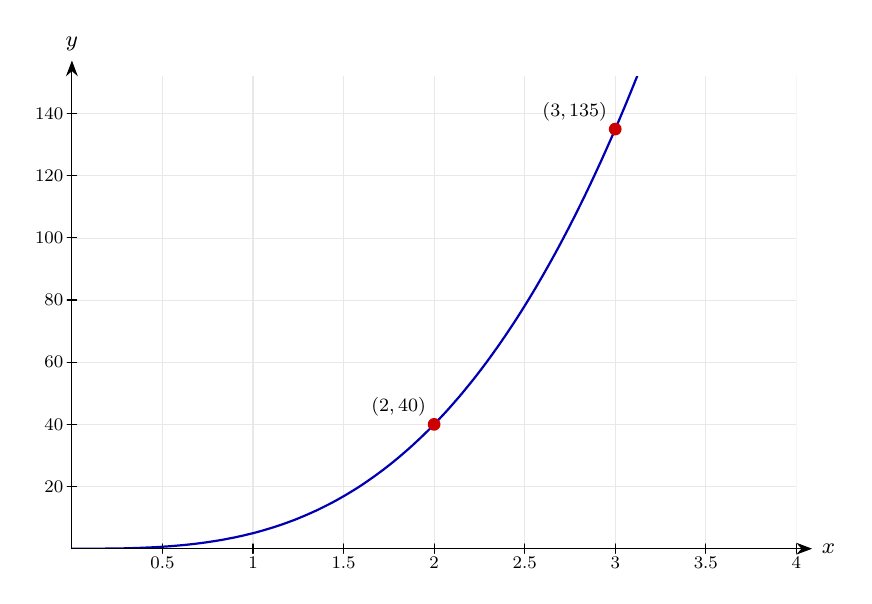
\begin{tikzpicture}[>={Stealth[length=2mm]},font=\footnotesize,line cap=round,line join=round]
\begin{scope}
\clip (0,0) rectangle (9.2,6);
\draw[gray!18] (0,0) grid[xstep=1.15,ystep=0.789] (9.2,6);
\draw[blue!70!black,thick] (0,0) -- (0.046,0) -- (0.092,0) -- (0.138,0) -- (0.184,0) -- (0.23,0) -- (0.276,0) -- (0.322,0.001) -- (0.368,0.001) -- (0.414,0.001) -- (0.46,0.002) -- (0.506,0.002) -- (0.552,0.003) -- (0.598,0.003) -- (0.644,0.004) -- (0.69,0.005) -- (0.736,0.006) -- (0.782,0.008) -- (0.828,0.009) -- (0.874,0.011) -- (0.92,0.013) -- (0.966,0.015) -- (1.012,0.017) -- (1.058,0.019) -- (1.104,0.022) -- (1.15,0.025) -- (1.196,0.028) -- (1.242,0.031) -- (1.288,0.035) -- (1.334,0.039) -- (1.38,0.043) -- (1.426,0.047) -- (1.472,0.052) -- (1.518,0.057) -- (1.564,0.062) -- (1.61,0.068) -- (1.656,0.074) -- (1.702,0.08) -- (1.748,0.087) -- (1.794,0.094) -- (1.84,0.101) -- (1.886,0.109) -- (1.932,0.117) -- (1.978,0.126) -- (2.024,0.135) -- (2.07,0.144) -- (2.116,0.154) -- (2.162,0.164) -- (2.208,0.175) -- (2.254,0.186) -- (2.3,0.197) -- (2.346,0.209) -- (2.392,0.222) -- (2.438,0.235) -- (2.484,0.249) -- (2.53,0.263) -- (2.576,0.277) -- (2.622,0.292) -- (2.668,0.308) -- (2.714,0.324) -- (2.76,0.341) -- (2.806,0.358) -- (2.852,0.376) -- (2.898,0.395) -- (2.944,0.414) -- (2.99,0.434) -- (3.036,0.454) -- (3.082,0.475) -- (3.128,0.496) -- (3.174,0.519) -- (3.22,0.542) -- (3.266,0.565) -- (3.312,0.589) -- (3.358,0.614) -- (3.404,0.64) -- (3.45,0.666) -- (3.496,0.693) -- (3.542,0.721) -- (3.588,0.749) -- (3.634,0.778) -- (3.68,0.808) -- (3.726,0.839) -- (3.772,0.871) -- (3.818,0.903) -- (3.864,0.936) -- (3.91,0.97) -- (3.956,1.004) -- (4.002,1.04) -- (4.048,1.076) -- (4.094,1.113) -- (4.14,1.151) -- (4.186,1.19) -- (4.232,1.23) -- (4.278,1.27) -- (4.324,1.311) -- (4.37,1.354) -- (4.416,1.397) -- (4.462,1.441) -- (4.508,1.486) -- (4.554,1.532) -- (4.6,1.579) -- (4.646,1.627) -- (4.692,1.676) -- (4.738,1.725) -- (4.784,1.776) -- (4.83,1.828) -- (4.876,1.881) -- (4.922,1.934) -- (4.968,1.989) -- (5.014,2.045) -- (5.06,2.102) -- (5.106,2.159) -- (5.152,2.218) -- (5.198,2.278) -- (5.244,2.339) -- (5.29,2.401) -- (5.336,2.465) -- (5.382,2.529) -- (5.428,2.594) -- (5.474,2.661) -- (5.52,2.728) -- (5.566,2.797) -- (5.612,2.867) -- (5.658,2.938) -- (5.704,3.01) -- (5.75,3.084) -- (5.796,3.158) -- (5.842,3.234) -- (5.888,3.311) -- (5.934,3.39) -- (5.98,3.469) -- (6.026,3.55) -- (6.072,3.632) -- (6.118,3.715) -- (6.164,3.799) -- (6.21,3.885) -- (6.256,3.972) -- (6.302,4.06) -- (6.348,4.15) -- (6.394,4.24) -- (6.44,4.333) -- (6.486,4.426) -- (6.532,4.521) -- (6.578,4.617) -- (6.624,4.715) -- (6.67,4.814) -- (6.716,4.914) -- (6.762,5.016) -- (6.808,5.119) -- (6.854,5.223) -- (6.9,5.329) -- (6.946,5.436) -- (6.992,5.545) -- (7.038,5.655) -- (7.084,5.767) -- (7.13,5.88) -- (7.176,5.994) -- (7.222,6.11) -- (7.268,6.228) -- (7.314,6.347) -- (7.36,6.467) -- (7.406,6.589) -- (7.452,6.713) -- (7.498,6.838) -- (7.544,6.965) -- (7.59,7.093) -- (7.636,7.223) -- (7.682,7.354) -- (7.728,7.487) -- (7.774,7.621) -- (7.82,7.757) -- (7.866,7.895) -- (7.912,8.034) -- (7.958,8.175) -- (8.004,8.318) -- (8.05,8.462) -- (8.096,8.608) -- (8.142,8.756) -- (8.188,8.905) -- (8.234,9.056) -- (8.28,9.208) -- (8.326,9.363) -- (8.372,9.519) -- (8.418,9.677) -- (8.464,9.836) -- (8.51,9.997) -- (8.556,10.16) -- (8.602,10.325) -- (8.648,10.492) -- (8.694,10.66) -- (8.74,10.83) -- (8.786,11.002) -- (8.832,11.176) -- (8.878,11.351) -- (8.924,11.529) -- (8.97,11.708) -- (9.016,11.889) -- (9.062,12) -- (9.108,12) -- (9.154,12) -- (9.2,12);
\end{scope}
\draw[->] (0,0) -- (9.4,0) node[right]{$x$};
\draw[->] (0,0) -- (0,6.2) node[above]{$y$};
\draw (1.15,-0.06) -- (1.15,0.06) node[below=2pt,scale=0.8]{$0.5$};
\draw (2.3,-0.06) -- (2.3,0.06) node[below=2pt,scale=0.8]{$1$};
\draw (3.45,-0.06) -- (3.45,0.06) node[below=2pt,scale=0.8]{$1.5$};
\draw (4.6,-0.06) -- (4.6,0.06) node[below=2pt,scale=0.8]{$2$};
\draw (5.75,-0.06) -- (5.75,0.06) node[below=2pt,scale=0.8]{$2.5$};
\draw (6.9,-0.06) -- (6.9,0.06) node[below=2pt,scale=0.8]{$3$};
\draw (8.05,-0.06) -- (8.05,0.06) node[below=2pt,scale=0.8]{$3.5$};
\draw (9.2,-0.06) -- (9.2,0.06) node[below=2pt,scale=0.8]{$4$};
\draw (-0.06,0.789) -- (0.06,0.789) node[left=2pt,scale=0.8]{$20$};
\draw (-0.06,1.579) -- (0.06,1.579) node[left=2pt,scale=0.8]{$40$};
\draw (-0.06,2.368) -- (0.06,2.368) node[left=2pt,scale=0.8]{$60$};
\draw (-0.06,3.158) -- (0.06,3.158) node[left=2pt,scale=0.8]{$80$};
\draw (-0.06,3.947) -- (0.06,3.947) node[left=2pt,scale=0.8]{$100$};
\draw (-0.06,4.737) -- (0.06,4.737) node[left=2pt,scale=0.8]{$120$};
\draw (-0.06,5.526) -- (0.06,5.526) node[left=2pt,scale=0.8]{$140$};
\fill[red!80!black] (4.6,1.579) circle (2.3pt);
\node[above left,scale=0.85] at (4.6,1.579) {$(2,40)$};
\fill[red!80!black] (6.9,5.329) circle (2.3pt);
\node[above left,scale=0.85] at (6.9,5.329) {$(3,135)$};
\end{tikzpicture}
}
\end{center}
\small The relationship plotted, with the data points marked.\normalsize

\medskip\hrule

\section*{Proportion 42\quad\small\texttt{(cg4-042)}}
\addcontentsline{toc}{section}{Proportion 42 (cg4-042)}
\textit{Difficulty: Foundation \quad\textbar\quad Marks: 3}

\question{The time \( T \) to travel a fixed distance is inversely proportional to speed \( s \). At 60 km/h the journey takes 2 hours. How long at 80 km/h?}

\textbf{Worked solution.}

\textit{Step 1: Find k}
\[\begin{gathered}
T = \frac{k}{s} \implies 2 = \frac{k}{60} \implies k = 120
\end{gathered}\]
Inverse proportion gives \( T = \frac{k}{s} \). Here \( k \) is the fixed distance in km (since distance = speed $\times$ time). Multiply both sides by 60.

\textit{Step 2: Find T}
\[\begin{gathered}
T = \frac{120}{80} = 1.5 \text{ hours}
\end{gathered}\]
Sense-check: a higher speed (80 vs 60) should give a shorter time, and 1.5 < 2 hours, so this is consistent.

\begin{answerbox}
\textbf{Final answer:}\quad \(\displaystyle 1.5\) hours (1 hour 30 minutes)
\end{answerbox}
\textbf{Graph.}

\begin{center}
\resizebox{\ifdim\width>\linewidth \linewidth\else \width\fi}{!}{%
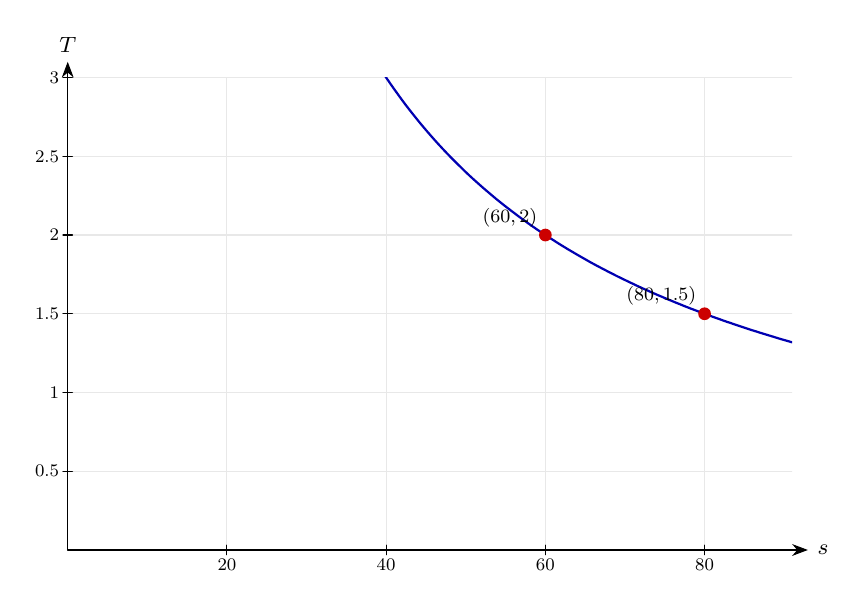
\begin{tikzpicture}[>={Stealth[length=2mm]},font=\footnotesize,line cap=round,line join=round]
\begin{scope}
\clip (0,0) rectangle (9.2,6);
\draw[gray!18] (0,0) grid[xstep=2.022,ystep=1] (9.2,6);
\draw[blue!70!black,thick] (0.023,12) -- (0.069,12) -- (0.115,12) -- (0.161,12) -- (0.207,12) -- (0.252,12) -- (0.298,12) -- (0.344,12) -- (0.39,12) -- (0.436,12) -- (0.482,12) -- (0.528,12) -- (0.574,12) -- (0.62,12) -- (0.665,12) -- (0.711,12) -- (0.757,12) -- (0.803,12) -- (0.849,12) -- (0.895,12) -- (0.941,12) -- (0.987,12) -- (1.032,12) -- (1.078,12) -- (1.124,12) -- (1.17,12) -- (1.216,12) -- (1.262,12) -- (1.308,12) -- (1.354,12) -- (1.4,12) -- (1.445,12) -- (1.491,12) -- (1.537,12) -- (1.583,12) -- (1.629,12) -- (1.675,12) -- (1.721,12) -- (1.767,12) -- (1.813,12) -- (1.858,12) -- (1.904,12) -- (1.95,12) -- (1.996,12) -- (2.042,11.883) -- (2.088,11.622) -- (2.134,11.372) -- (2.18,11.132) -- (2.225,10.903) -- (2.271,10.682) -- (2.317,10.471) -- (2.363,10.268) -- (2.409,10.072) -- (2.455,9.884) -- (2.501,9.702) -- (2.547,9.528) -- (2.593,9.359) -- (2.638,9.196) -- (2.684,9.039) -- (2.73,8.887) -- (2.776,8.74) -- (2.822,8.598) -- (2.868,8.461) -- (2.914,8.327) -- (2.96,8.198) -- (3.006,8.073) -- (3.051,7.952) -- (3.097,7.834) -- (3.143,7.719) -- (3.189,7.608) -- (3.235,7.5) -- (3.281,7.396) -- (3.327,7.294) -- (3.373,7.194) -- (3.418,7.098) -- (3.464,7.004) -- (3.51,6.912) -- (3.556,6.823) -- (3.602,6.736) -- (3.648,6.651) -- (3.694,6.569) -- (3.74,6.488) -- (3.786,6.41) -- (3.831,6.333) -- (3.877,6.258) -- (3.923,6.185) -- (3.969,6.113) -- (4.015,6.043) -- (4.061,5.975) -- (4.107,5.908) -- (4.153,5.843) -- (4.199,5.779) -- (4.244,5.717) -- (4.29,5.655) -- (4.336,5.596) -- (4.382,5.537) -- (4.428,5.48) -- (4.474,5.423) -- (4.52,5.368) -- (4.566,5.314) -- (4.611,5.262) -- (4.657,5.21) -- (4.703,5.159) -- (4.749,5.109) -- (4.795,5.06) -- (4.841,5.012) -- (4.887,4.965) -- (4.933,4.919) -- (4.979,4.874) -- (5.024,4.829) -- (5.07,4.785) -- (5.116,4.742) -- (5.162,4.7) -- (5.208,4.659) -- (5.254,4.618) -- (5.3,4.578) -- (5.346,4.539) -- (5.392,4.5) -- (5.437,4.462) -- (5.483,4.425) -- (5.529,4.388) -- (5.575,4.352) -- (5.621,4.317) -- (5.667,4.282) -- (5.713,4.247) -- (5.759,4.213) -- (5.805,4.18) -- (5.85,4.147) -- (5.896,4.115) -- (5.942,4.083) -- (5.988,4.052) -- (6.034,4.021) -- (6.08,3.991) -- (6.126,3.961) -- (6.172,3.932) -- (6.217,3.903) -- (6.263,3.874) -- (6.309,3.846) -- (6.355,3.818) -- (6.401,3.791) -- (6.447,3.764) -- (6.493,3.737) -- (6.539,3.711) -- (6.585,3.685) -- (6.63,3.659) -- (6.676,3.634) -- (6.722,3.609) -- (6.768,3.585) -- (6.814,3.561) -- (6.86,3.537) -- (6.906,3.514) -- (6.952,3.49) -- (6.998,3.467) -- (7.043,3.445) -- (7.089,3.423) -- (7.135,3.401) -- (7.181,3.379) -- (7.227,3.357) -- (7.273,3.336) -- (7.319,3.315) -- (7.365,3.295) -- (7.41,3.274) -- (7.456,3.254) -- (7.502,3.234) -- (7.548,3.215) -- (7.594,3.195) -- (7.64,3.176) -- (7.686,3.157) -- (7.732,3.138) -- (7.778,3.12) -- (7.823,3.101) -- (7.869,3.083) -- (7.915,3.065) -- (7.961,3.048) -- (8.007,3.03) -- (8.053,3.013) -- (8.099,2.996) -- (8.145,2.979) -- (8.191,2.962) -- (8.236,2.946) -- (8.282,2.93) -- (8.328,2.913) -- (8.374,2.897) -- (8.42,2.882) -- (8.466,2.866) -- (8.512,2.851) -- (8.558,2.835) -- (8.603,2.82) -- (8.649,2.805) -- (8.695,2.79) -- (8.741,2.776) -- (8.787,2.761) -- (8.833,2.747) -- (8.879,2.733) -- (8.925,2.719) -- (8.971,2.705) -- (9.016,2.691) -- (9.062,2.677) -- (9.108,2.664) -- (9.154,2.651) -- (9.2,2.637);
\end{scope}
\draw[->] (0,0) -- (9.4,0) node[right]{$s$};
\draw[->] (0,0) -- (0,6.2) node[above]{$T$};
\draw (2.022,-0.06) -- (2.022,0.06) node[below=2pt,scale=0.8]{$20$};
\draw (4.044,-0.06) -- (4.044,0.06) node[below=2pt,scale=0.8]{$40$};
\draw (6.066,-0.06) -- (6.066,0.06) node[below=2pt,scale=0.8]{$60$};
\draw (8.088,-0.06) -- (8.088,0.06) node[below=2pt,scale=0.8]{$80$};
\draw (-0.06,1) -- (0.06,1) node[left=2pt,scale=0.8]{$0.5$};
\draw (-0.06,2) -- (0.06,2) node[left=2pt,scale=0.8]{$1$};
\draw (-0.06,3) -- (0.06,3) node[left=2pt,scale=0.8]{$1.5$};
\draw (-0.06,4) -- (0.06,4) node[left=2pt,scale=0.8]{$2$};
\draw (-0.06,5) -- (0.06,5) node[left=2pt,scale=0.8]{$2.5$};
\draw (-0.06,6) -- (0.06,6) node[left=2pt,scale=0.8]{$3$};
\fill[red!80!black] (6.066,4) circle (2.3pt);
\node[above left,scale=0.85] at (6.066,4) {$(60,2)$};
\fill[red!80!black] (8.088,3) circle (2.3pt);
\node[above left,scale=0.85] at (8.088,3) {$(80,1.5)$};
\end{tikzpicture}
}
\end{center}
\small The relationship plotted, with the data points marked.\normalsize

\medskip\hrule

\section*{Proportion 43\quad\small\texttt{(cg4-043)}}
\addcontentsline{toc}{section}{Proportion 43 (cg4-043)}
\textit{Difficulty: Foundation \quad\textbar\quad Marks: 4}

\question{\( P \) is proportional to \( \sqrt{Q} \). When \( Q = 25 \), \( P = 10 \). Find \( Q \) when \( P = 14 \).}

\textbf{Worked solution.}

\textit{Step 1: Find k}
\[\begin{gathered}
P = k\sqrt{Q} \implies 10 = 5k \implies k = 2
\end{gathered}\]
\( P \propto \sqrt{Q} \) translates to \( P = k\sqrt{Q} \). Take \( \sqrt{25} = 5 \) first, then divide both sides by 5.

\textit{Step 2: Find Q}
\[\begin{gathered}
14 = 2\sqrt{Q} \implies \sqrt{Q} = 7 \implies Q = 49
\end{gathered}\]
Divide by 2 to isolate \( \sqrt{Q} \), then square both sides to get \( Q \). Squaring last avoids working with \( Q \) under a root.

\begin{answerbox}
\textbf{Final answer:}\quad \(\displaystyle Q = 49\)
\end{answerbox}
\textbf{Graph.}

\begin{center}
\resizebox{\ifdim\width>\linewidth \linewidth\else \width\fi}{!}{%
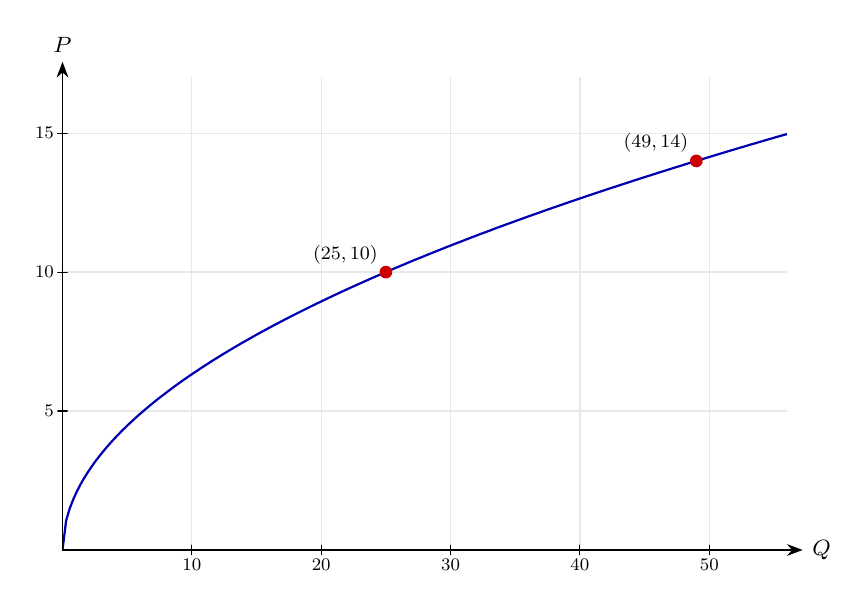
\begin{tikzpicture}[>={Stealth[length=2mm]},font=\footnotesize,line cap=round,line join=round]
\begin{scope}
\clip (0,0) rectangle (9.2,6);
\draw[gray!18] (0,0) grid[xstep=1.643,ystep=1.765] (9.2,6);
\draw[blue!70!black,thick] (0,0) -- (0.046,0.374) -- (0.092,0.528) -- (0.138,0.647) -- (0.184,0.747) -- (0.23,0.835) -- (0.276,0.915) -- (0.322,0.988) -- (0.368,1.056) -- (0.414,1.121) -- (0.46,1.181) -- (0.506,1.239) -- (0.552,1.294) -- (0.598,1.347) -- (0.644,1.398) -- (0.69,1.447) -- (0.736,1.494) -- (0.782,1.54) -- (0.828,1.585) -- (0.874,1.628) -- (0.92,1.67) -- (0.966,1.712) -- (1.012,1.752) -- (1.058,1.791) -- (1.104,1.83) -- (1.15,1.868) -- (1.196,1.905) -- (1.242,1.941) -- (1.288,1.976) -- (1.334,2.011) -- (1.38,2.046) -- (1.426,2.08) -- (1.472,2.113) -- (1.518,2.146) -- (1.564,2.178) -- (1.61,2.21) -- (1.656,2.241) -- (1.702,2.272) -- (1.748,2.303) -- (1.794,2.333) -- (1.84,2.362) -- (1.886,2.392) -- (1.932,2.421) -- (1.978,2.449) -- (2.024,2.478) -- (2.07,2.506) -- (2.116,2.533) -- (2.162,2.561) -- (2.208,2.588) -- (2.254,2.615) -- (2.3,2.641) -- (2.346,2.667) -- (2.392,2.693) -- (2.438,2.719) -- (2.484,2.745) -- (2.53,2.77) -- (2.576,2.795) -- (2.622,2.82) -- (2.668,2.845) -- (2.714,2.869) -- (2.76,2.893) -- (2.806,2.917) -- (2.852,2.941) -- (2.898,2.965) -- (2.944,2.988) -- (2.99,3.011) -- (3.036,3.034) -- (3.082,3.057) -- (3.128,3.08) -- (3.174,3.103) -- (3.22,3.125) -- (3.266,3.147) -- (3.312,3.169) -- (3.358,3.191) -- (3.404,3.213) -- (3.45,3.235) -- (3.496,3.256) -- (3.542,3.278) -- (3.588,3.299) -- (3.634,3.32) -- (3.68,3.341) -- (3.726,3.362) -- (3.772,3.382) -- (3.818,3.403) -- (3.864,3.423) -- (3.91,3.444) -- (3.956,3.464) -- (4.002,3.484) -- (4.048,3.504) -- (4.094,3.524) -- (4.14,3.544) -- (4.186,3.563) -- (4.232,3.583) -- (4.278,3.602) -- (4.324,3.621) -- (4.37,3.641) -- (4.416,3.66) -- (4.462,3.679) -- (4.508,3.698) -- (4.554,3.716) -- (4.6,3.735) -- (4.646,3.754) -- (4.692,3.772) -- (4.738,3.791) -- (4.784,3.809) -- (4.83,3.827) -- (4.876,3.846) -- (4.922,3.864) -- (4.968,3.882) -- (5.014,3.9) -- (5.06,3.917) -- (5.106,3.935) -- (5.152,3.953) -- (5.198,3.971) -- (5.244,3.988) -- (5.29,4.006) -- (5.336,4.023) -- (5.382,4.04) -- (5.428,4.057) -- (5.474,4.075) -- (5.52,4.092) -- (5.566,4.109) -- (5.612,4.126) -- (5.658,4.143) -- (5.704,4.159) -- (5.75,4.176) -- (5.796,4.193) -- (5.842,4.209) -- (5.888,4.226) -- (5.934,4.242) -- (5.98,4.259) -- (6.026,4.275) -- (6.072,4.291) -- (6.118,4.308) -- (6.164,4.324) -- (6.21,4.34) -- (6.256,4.356) -- (6.302,4.372) -- (6.348,4.388) -- (6.394,4.404) -- (6.44,4.42) -- (6.486,4.435) -- (6.532,4.451) -- (6.578,4.467) -- (6.624,4.482) -- (6.67,4.498) -- (6.716,4.513) -- (6.762,4.529) -- (6.808,4.544) -- (6.854,4.559) -- (6.9,4.575) -- (6.946,4.59) -- (6.992,4.605) -- (7.038,4.62) -- (7.084,4.635) -- (7.13,4.65) -- (7.176,4.665) -- (7.222,4.68) -- (7.268,4.695) -- (7.314,4.71) -- (7.36,4.725) -- (7.406,4.739) -- (7.452,4.754) -- (7.498,4.769) -- (7.544,4.783) -- (7.59,4.798) -- (7.636,4.812) -- (7.682,4.827) -- (7.728,4.841) -- (7.774,4.856) -- (7.82,4.87) -- (7.866,4.884) -- (7.912,4.899) -- (7.958,4.913) -- (8.004,4.927) -- (8.05,4.941) -- (8.096,4.955) -- (8.142,4.969) -- (8.188,4.983) -- (8.234,4.997) -- (8.28,5.011) -- (8.326,5.025) -- (8.372,5.039) -- (8.418,5.053) -- (8.464,5.067) -- (8.51,5.08) -- (8.556,5.094) -- (8.602,5.108) -- (8.648,5.121) -- (8.694,5.135) -- (8.74,5.149) -- (8.786,5.162) -- (8.832,5.176) -- (8.878,5.189) -- (8.924,5.203) -- (8.97,5.216) -- (9.016,5.229) -- (9.062,5.243) -- (9.108,5.256) -- (9.154,5.269) -- (9.2,5.282);
\end{scope}
\draw[->] (0,0) -- (9.4,0) node[right]{$Q$};
\draw[->] (0,0) -- (0,6.2) node[above]{$P$};
\draw (1.643,-0.06) -- (1.643,0.06) node[below=2pt,scale=0.8]{$10$};
\draw (3.286,-0.06) -- (3.286,0.06) node[below=2pt,scale=0.8]{$20$};
\draw (4.929,-0.06) -- (4.929,0.06) node[below=2pt,scale=0.8]{$30$};
\draw (6.571,-0.06) -- (6.571,0.06) node[below=2pt,scale=0.8]{$40$};
\draw (8.214,-0.06) -- (8.214,0.06) node[below=2pt,scale=0.8]{$50$};
\draw (-0.06,1.765) -- (0.06,1.765) node[left=2pt,scale=0.8]{$5$};
\draw (-0.06,3.529) -- (0.06,3.529) node[left=2pt,scale=0.8]{$10$};
\draw (-0.06,5.294) -- (0.06,5.294) node[left=2pt,scale=0.8]{$15$};
\fill[red!80!black] (4.107,3.529) circle (2.3pt);
\node[above left,scale=0.85] at (4.107,3.529) {$(25,10)$};
\fill[red!80!black] (8.05,4.941) circle (2.3pt);
\node[above left,scale=0.85] at (8.05,4.941) {$(49,14)$};
\end{tikzpicture}
}
\end{center}
\small The relationship plotted, with the data points marked.\normalsize

\medskip\hrule

\section*{Proportion 44\quad\small\texttt{(cg4-044)}}
\addcontentsline{toc}{section}{Proportion 44 (cg4-044)}
\textit{Difficulty: Foundation \quad\textbar\quad Marks: 3}

\question{\( y \) is inversely proportional to \( x^2 \). When \( x = 2 \), \( y = 5 \). Find \( y \) when \( x = 10 \).}

\textbf{Worked solution.}

\textit{Step 1: Find k}
\[\begin{gathered}
y = \frac{k}{x^2} \implies 5 = \frac{k}{4} \implies k = 20
\end{gathered}\]
\( y \propto \frac{1}{x^2} \) means \( y = \frac{k}{x^2} \). Square \( x = 2 \) to get 4, then multiply both sides by 4 to clear the fraction.

\textit{Step 2: Find y}
\[\begin{gathered}
y = \frac{20}{100} = 0.2
\end{gathered}\]
\( x \) increased 5-fold, so \( x^2 \) grew 25-fold and \( y \) shrank by a factor of 25 (from 5 to 0.2). That matches the inverse-square law.

\begin{answerbox}
\textbf{Final answer:}\quad \(\displaystyle y = 0.2\)
\end{answerbox}
\textbf{Graph.}

\begin{center}
\resizebox{\ifdim\width>\linewidth \linewidth\else \width\fi}{!}{%
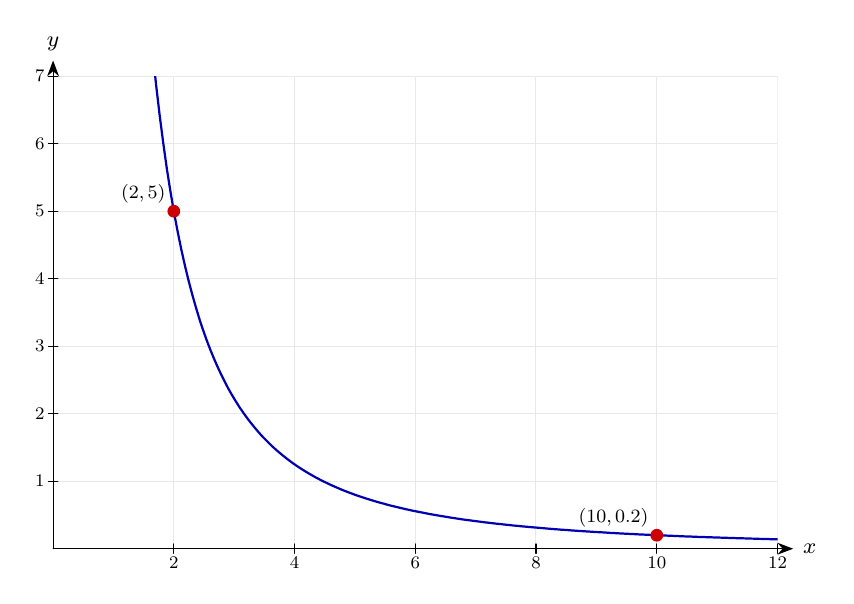
\begin{tikzpicture}[>={Stealth[length=2mm]},font=\footnotesize,line cap=round,line join=round]
\begin{scope}
\clip (0,0) rectangle (9.2,6);
\draw[gray!18] (0,0) grid[xstep=1.533,ystep=0.857] (9.2,6);
\draw[blue!70!black,thick] (0.023,12) -- (0.069,12) -- (0.115,12) -- (0.161,12) -- (0.207,12) -- (0.252,12) -- (0.298,12) -- (0.344,12) -- (0.39,12) -- (0.436,12) -- (0.482,12) -- (0.528,12) -- (0.574,12) -- (0.62,12) -- (0.665,12) -- (0.711,12) -- (0.757,12) -- (0.803,12) -- (0.849,12) -- (0.895,12) -- (0.941,11.387) -- (0.987,10.352) -- (1.032,9.452) -- (1.078,8.665) -- (1.124,7.972) -- (1.17,7.359) -- (1.216,6.814) -- (1.262,6.328) -- (1.308,5.892) -- (1.354,5.499) -- (1.4,5.144) -- (1.445,4.823) -- (1.491,4.531) -- (1.537,4.264) -- (1.583,4.021) -- (1.629,3.797) -- (1.675,3.592) -- (1.721,3.403) -- (1.767,3.229) -- (1.813,3.067) -- (1.858,2.918) -- (1.904,2.779) -- (1.95,2.649) -- (1.996,2.529) -- (2.042,2.417) -- (2.088,2.312) -- (2.134,2.213) -- (2.18,2.121) -- (2.225,2.034) -- (2.271,1.953) -- (2.317,1.877) -- (2.363,1.804) -- (2.409,1.736) -- (2.455,1.672) -- (2.501,1.611) -- (2.547,1.554) -- (2.593,1.499) -- (2.638,1.447) -- (2.684,1.398) -- (2.73,1.352) -- (2.776,1.307) -- (2.822,1.265) -- (2.868,1.225) -- (2.914,1.187) -- (2.96,1.15) -- (3.006,1.115) -- (3.051,1.082) -- (3.097,1.05) -- (3.143,1.02) -- (3.189,0.991) -- (3.235,0.963) -- (3.281,0.936) -- (3.327,0.91) -- (3.373,0.886) -- (3.418,0.862) -- (3.464,0.84) -- (3.51,0.818) -- (3.556,0.797) -- (3.602,0.777) -- (3.648,0.757) -- (3.694,0.738) -- (3.74,0.72) -- (3.786,0.703) -- (3.831,0.686) -- (3.877,0.67) -- (3.923,0.655) -- (3.969,0.64) -- (4.015,0.625) -- (4.061,0.611) -- (4.107,0.597) -- (4.153,0.584) -- (4.199,0.572) -- (4.244,0.559) -- (4.29,0.547) -- (4.336,0.536) -- (4.382,0.525) -- (4.428,0.514) -- (4.474,0.503) -- (4.52,0.493) -- (4.566,0.483) -- (4.612,0.474) -- (4.657,0.465) -- (4.703,0.456) -- (4.749,0.447) -- (4.795,0.438) -- (4.841,0.43) -- (4.887,0.422) -- (4.933,0.414) -- (4.979,0.407) -- (5.024,0.399) -- (5.07,0.392) -- (5.116,0.385) -- (5.162,0.378) -- (5.208,0.371) -- (5.254,0.365) -- (5.3,0.359) -- (5.346,0.353) -- (5.392,0.347) -- (5.437,0.341) -- (5.483,0.335) -- (5.529,0.33) -- (5.575,0.324) -- (5.621,0.319) -- (5.667,0.314) -- (5.713,0.309) -- (5.759,0.304) -- (5.805,0.299) -- (5.85,0.294) -- (5.896,0.29) -- (5.942,0.285) -- (5.988,0.281) -- (6.034,0.277) -- (6.08,0.273) -- (6.126,0.269) -- (6.172,0.265) -- (6.217,0.261) -- (6.263,0.257) -- (6.309,0.253) -- (6.355,0.249) -- (6.401,0.246) -- (6.447,0.242) -- (6.493,0.239) -- (6.539,0.236) -- (6.585,0.232) -- (6.63,0.229) -- (6.676,0.226) -- (6.722,0.223) -- (6.768,0.22) -- (6.814,0.217) -- (6.86,0.214) -- (6.906,0.211) -- (6.952,0.209) -- (6.998,0.206) -- (7.043,0.203) -- (7.089,0.2) -- (7.135,0.198) -- (7.181,0.195) -- (7.227,0.193) -- (7.273,0.19) -- (7.319,0.188) -- (7.365,0.186) -- (7.41,0.183) -- (7.456,0.181) -- (7.502,0.179) -- (7.548,0.177) -- (7.594,0.175) -- (7.64,0.173) -- (7.686,0.171) -- (7.732,0.169) -- (7.778,0.167) -- (7.823,0.165) -- (7.869,0.163) -- (7.915,0.161) -- (7.961,0.159) -- (8.007,0.157) -- (8.053,0.155) -- (8.099,0.154) -- (8.145,0.152) -- (8.191,0.15) -- (8.236,0.149) -- (8.282,0.147) -- (8.328,0.145) -- (8.374,0.144) -- (8.42,0.142) -- (8.466,0.141) -- (8.512,0.139) -- (8.558,0.138) -- (8.603,0.136) -- (8.649,0.135) -- (8.695,0.133) -- (8.741,0.132) -- (8.787,0.131) -- (8.833,0.129) -- (8.879,0.128) -- (8.925,0.127) -- (8.971,0.125) -- (9.016,0.124) -- (9.062,0.123) -- (9.108,0.121) -- (9.154,0.12) -- (9.2,0.119);
\end{scope}
\draw[->] (0,0) -- (9.4,0) node[right]{$x$};
\draw[->] (0,0) -- (0,6.2) node[above]{$y$};
\draw (1.533,-0.06) -- (1.533,0.06) node[below=2pt,scale=0.8]{$2$};
\draw (3.067,-0.06) -- (3.067,0.06) node[below=2pt,scale=0.8]{$4$};
\draw (4.6,-0.06) -- (4.6,0.06) node[below=2pt,scale=0.8]{$6$};
\draw (6.133,-0.06) -- (6.133,0.06) node[below=2pt,scale=0.8]{$8$};
\draw (7.667,-0.06) -- (7.667,0.06) node[below=2pt,scale=0.8]{$10$};
\draw (9.2,-0.06) -- (9.2,0.06) node[below=2pt,scale=0.8]{$12$};
\draw (-0.06,0.857) -- (0.06,0.857) node[left=2pt,scale=0.8]{$1$};
\draw (-0.06,1.714) -- (0.06,1.714) node[left=2pt,scale=0.8]{$2$};
\draw (-0.06,2.571) -- (0.06,2.571) node[left=2pt,scale=0.8]{$3$};
\draw (-0.06,3.429) -- (0.06,3.429) node[left=2pt,scale=0.8]{$4$};
\draw (-0.06,4.286) -- (0.06,4.286) node[left=2pt,scale=0.8]{$5$};
\draw (-0.06,5.143) -- (0.06,5.143) node[left=2pt,scale=0.8]{$6$};
\draw (-0.06,6) -- (0.06,6) node[left=2pt,scale=0.8]{$7$};
\fill[red!80!black] (1.533,4.286) circle (2.3pt);
\node[above left,scale=0.85] at (1.533,4.286) {$(2,5)$};
\fill[red!80!black] (7.667,0.171) circle (2.3pt);
\node[above left,scale=0.85] at (7.667,0.171) {$(10,0.2)$};
\end{tikzpicture}
}
\end{center}
\small The relationship plotted, with the data points marked.\normalsize

\medskip\hrule

\section*{Proportion 45\quad\small\texttt{(cg4-045)}}
\addcontentsline{toc}{section}{Proportion 45 (cg4-045)}
\textit{Difficulty: Foundation \quad\textbar\quad Marks: 3}

\question{If \( x \) is doubled, what happens to \( y \) when: (a) \( y \propto x \); (b) \( y \propto x^2 \); (c) \( y \propto \frac{1}{x} \)?}

\textbf{Worked solution.}

\textit{Step 1: (a) y = kx}
\[\begin{gathered}
y_{\text{new}} = k(2x) = 2kx = 2y
\end{gathered}\]
Replace \( x \) with \( 2x \) in \( y = kx \). The factor of 2 pulls out directly, so the new value is exactly twice the old --- \( y \) doubles.

\textit{Step 2: (b) y = kx\textasciicircum 2}
\[\begin{gathered}
y_{\text{new}} = k(2x)^2 = 4kx^2 = 4y
\end{gathered}\]
Crucially \( (2x)^2 = 4x^2 \), not \( 2x^2 \) --- the bracket squares both the 2 and the \( x \). So \( y \) is multiplied by 4.

\textit{Step 3: (c) y = k/x}
\[\begin{gathered}
y_{\text{new}} = \frac{k}{2x} = \frac{y}{2}
\end{gathered}\]
The 2 ends up on the denominator, so \( y \) is divided by 2. Doubling \( x \) halves \( y \) for inverse proportion.

\begin{answerbox}
\textbf{Final answer:}\quad (a) doubles; (b) quadruples; (c) halves
\end{answerbox}
\textbf{Graph.}

\begin{center}
\resizebox{\ifdim\width>\linewidth \linewidth\else \width\fi}{!}{%
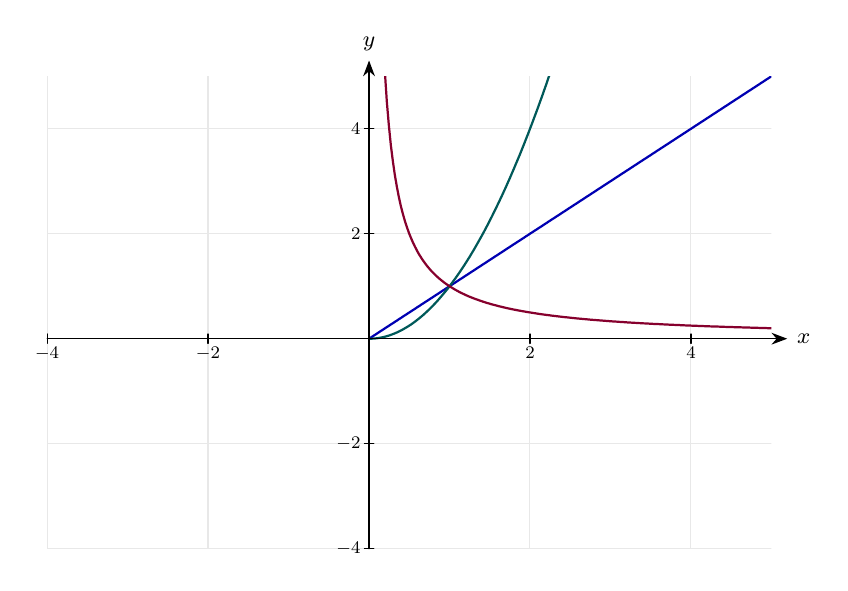
\begin{tikzpicture}[>={Stealth[length=2mm]},font=\footnotesize,line cap=round,line join=round]
\begin{scope}
\clip (0,0) rectangle (9.2,6);
\draw[gray!18] (0,0) grid[xstep=2.044,ystep=1.333] (9.2,6);
\draw[blue!70!black,thick] (4.089,2.667) -- (4.114,2.683) -- (4.14,2.7) -- (4.166,2.717) -- (4.191,2.733) -- (4.217,2.75) -- (4.242,2.767) -- (4.268,2.783) -- (4.293,2.8) -- (4.319,2.817) -- (4.344,2.833) -- (4.37,2.85) -- (4.396,2.867) -- (4.421,2.883) -- (4.447,2.9) -- (4.472,2.917) -- (4.498,2.933) -- (4.523,2.95) -- (4.549,2.967) -- (4.574,2.983) -- (4.6,3) -- (4.626,3.017) -- (4.651,3.033) -- (4.677,3.05) -- (4.702,3.067) -- (4.728,3.083) -- (4.753,3.1) -- (4.779,3.117) -- (4.804,3.133) -- (4.83,3.15) -- (4.856,3.167) -- (4.881,3.183) -- (4.907,3.2) -- (4.932,3.217) -- (4.958,3.233) -- (4.983,3.25) -- (5.009,3.267) -- (5.034,3.283) -- (5.06,3.3) -- (5.086,3.317) -- (5.111,3.333) -- (5.137,3.35) -- (5.162,3.367) -- (5.188,3.383) -- (5.213,3.4) -- (5.239,3.417) -- (5.264,3.433) -- (5.29,3.45) -- (5.316,3.467) -- (5.341,3.483) -- (5.367,3.5) -- (5.392,3.517) -- (5.418,3.533) -- (5.443,3.55) -- (5.469,3.567) -- (5.494,3.583) -- (5.52,3.6) -- (5.546,3.617) -- (5.571,3.633) -- (5.597,3.65) -- (5.622,3.667) -- (5.648,3.683) -- (5.673,3.7) -- (5.699,3.717) -- (5.724,3.733) -- (5.75,3.75) -- (5.776,3.767) -- (5.801,3.783) -- (5.827,3.8) -- (5.852,3.817) -- (5.878,3.833) -- (5.903,3.85) -- (5.929,3.867) -- (5.954,3.883) -- (5.98,3.9) -- (6.006,3.917) -- (6.031,3.933) -- (6.057,3.95) -- (6.082,3.967) -- (6.108,3.983) -- (6.133,4) -- (6.159,4.017) -- (6.184,4.033) -- (6.21,4.05) -- (6.236,4.067) -- (6.261,4.083) -- (6.287,4.1) -- (6.312,4.117) -- (6.338,4.133) -- (6.363,4.15) -- (6.389,4.167) -- (6.414,4.183) -- (6.44,4.2) -- (6.466,4.217) -- (6.491,4.233) -- (6.517,4.25) -- (6.542,4.267) -- (6.568,4.283) -- (6.593,4.3) -- (6.619,4.317) -- (6.644,4.333) -- (6.67,4.35) -- (6.696,4.367) -- (6.721,4.383) -- (6.747,4.4) -- (6.772,4.417) -- (6.798,4.433) -- (6.823,4.45) -- (6.849,4.467) -- (6.874,4.483) -- (6.9,4.5) -- (6.926,4.517) -- (6.951,4.533) -- (6.977,4.55) -- (7.002,4.567) -- (7.028,4.583) -- (7.053,4.6) -- (7.079,4.617) -- (7.104,4.633) -- (7.13,4.65) -- (7.156,4.667) -- (7.181,4.683) -- (7.207,4.7) -- (7.232,4.717) -- (7.258,4.733) -- (7.283,4.75) -- (7.309,4.767) -- (7.334,4.783) -- (7.36,4.8) -- (7.386,4.817) -- (7.411,4.833) -- (7.437,4.85) -- (7.462,4.867) -- (7.488,4.883) -- (7.513,4.9) -- (7.539,4.917) -- (7.564,4.933) -- (7.59,4.95) -- (7.616,4.967) -- (7.641,4.983) -- (7.667,5) -- (7.692,5.017) -- (7.718,5.033) -- (7.743,5.05) -- (7.769,5.067) -- (7.794,5.083) -- (7.82,5.1) -- (7.846,5.117) -- (7.871,5.133) -- (7.897,5.15) -- (7.922,5.167) -- (7.948,5.183) -- (7.973,5.2) -- (7.999,5.217) -- (8.024,5.233) -- (8.05,5.25) -- (8.076,5.267) -- (8.101,5.283) -- (8.127,5.3) -- (8.152,5.317) -- (8.178,5.333) -- (8.203,5.35) -- (8.229,5.367) -- (8.254,5.383) -- (8.28,5.4) -- (8.306,5.417) -- (8.331,5.433) -- (8.357,5.45) -- (8.382,5.467) -- (8.408,5.483) -- (8.433,5.5) -- (8.459,5.517) -- (8.484,5.533) -- (8.51,5.55) -- (8.536,5.567) -- (8.561,5.583) -- (8.587,5.6) -- (8.612,5.617) -- (8.638,5.633) -- (8.663,5.65) -- (8.689,5.667) -- (8.714,5.683) -- (8.74,5.7) -- (8.766,5.717) -- (8.791,5.733) -- (8.817,5.75) -- (8.842,5.767) -- (8.868,5.783) -- (8.893,5.8) -- (8.919,5.817) -- (8.944,5.833) -- (8.97,5.85) -- (8.996,5.867) -- (9.021,5.883) -- (9.047,5.9) -- (9.072,5.917) -- (9.098,5.933) -- (9.123,5.95) -- (9.149,5.967) -- (9.174,5.983) -- (9.2,6);
\draw[teal!70!black,thick] (4.089,2.667) -- (4.114,2.667) -- (4.14,2.668) -- (4.166,2.67) -- (4.191,2.673) -- (4.217,2.677) -- (4.242,2.682) -- (4.268,2.687) -- (4.293,2.693) -- (4.319,2.7) -- (4.344,2.708) -- (4.37,2.717) -- (4.396,2.727) -- (4.421,2.737) -- (4.447,2.748) -- (4.472,2.76) -- (4.498,2.773) -- (4.523,2.787) -- (4.549,2.802) -- (4.574,2.817) -- (4.6,2.833) -- (4.626,2.85) -- (4.651,2.868) -- (4.677,2.887) -- (4.702,2.907) -- (4.728,2.927) -- (4.753,2.948) -- (4.779,2.97) -- (4.804,2.993) -- (4.83,3.017) -- (4.856,3.042) -- (4.881,3.067) -- (4.907,3.093) -- (4.932,3.12) -- (4.958,3.148) -- (4.983,3.177) -- (5.009,3.207) -- (5.034,3.237) -- (5.06,3.268) -- (5.086,3.3) -- (5.111,3.333) -- (5.137,3.367) -- (5.162,3.402) -- (5.188,3.437) -- (5.213,3.473) -- (5.239,3.51) -- (5.264,3.548) -- (5.29,3.587) -- (5.316,3.627) -- (5.341,3.667) -- (5.367,3.708) -- (5.392,3.75) -- (5.418,3.793) -- (5.443,3.837) -- (5.469,3.882) -- (5.494,3.927) -- (5.52,3.973) -- (5.546,4.02) -- (5.571,4.068) -- (5.597,4.117) -- (5.622,4.167) -- (5.648,4.217) -- (5.673,4.268) -- (5.699,4.32) -- (5.724,4.373) -- (5.75,4.427) -- (5.776,4.482) -- (5.801,4.537) -- (5.827,4.593) -- (5.852,4.65) -- (5.878,4.708) -- (5.903,4.767) -- (5.929,4.827) -- (5.954,4.887) -- (5.98,4.948) -- (6.006,5.01) -- (6.031,5.073) -- (6.057,5.137) -- (6.082,5.202) -- (6.108,5.267) -- (6.133,5.333) -- (6.159,5.4) -- (6.184,5.468) -- (6.21,5.537) -- (6.236,5.607) -- (6.261,5.677) -- (6.287,5.748) -- (6.312,5.82) -- (6.338,5.893) -- (6.363,5.967) -- (6.389,6.042) -- (6.414,6.117) -- (6.44,6.193) -- (6.466,6.27) -- (6.491,6.348) -- (6.517,6.427) -- (6.542,6.507) -- (6.568,6.587) -- (6.593,6.668) -- (6.619,6.75) -- (6.644,6.833) -- (6.67,6.917) -- (6.696,7.002) -- (6.721,7.087) -- (6.747,7.173) -- (6.772,7.26) -- (6.798,7.348) -- (6.823,7.437) -- (6.849,7.527) -- (6.874,7.617) -- (6.9,7.708) -- (6.926,7.8) -- (6.951,7.893) -- (6.977,7.987) -- (7.002,8.082) -- (7.028,8.177) -- (7.053,8.273) -- (7.079,8.37) -- (7.104,8.468) -- (7.13,8.567) -- (7.156,8.667) -- (7.181,8.767) -- (7.207,8.868) -- (7.232,8.97) -- (7.258,9.073) -- (7.283,9.177) -- (7.309,9.282) -- (7.334,9.387) -- (7.36,9.493) -- (7.386,9.6) -- (7.411,9.708) -- (7.437,9.817) -- (7.462,9.927) -- (7.488,10.037) -- (7.513,10.148) -- (7.539,10.26) -- (7.564,10.373) -- (7.59,10.487) -- (7.616,10.602) -- (7.641,10.717) -- (7.667,10.833) -- (7.692,10.95) -- (7.718,11.068) -- (7.743,11.187) -- (7.769,11.307) -- (7.794,11.427) -- (7.82,11.548) -- (7.846,11.67) -- (7.871,11.793) -- (7.897,11.917) -- (7.922,12) -- (7.948,12) -- (7.973,12) -- (7.999,12) -- (8.024,12) -- (8.05,12) -- (8.076,12) -- (8.101,12) -- (8.127,12) -- (8.152,12) -- (8.178,12) -- (8.203,12) -- (8.229,12) -- (8.254,12) -- (8.28,12) -- (8.306,12) -- (8.331,12) -- (8.357,12) -- (8.382,12) -- (8.408,12) -- (8.433,12) -- (8.459,12) -- (8.484,12) -- (8.51,12) -- (8.536,12) -- (8.561,12) -- (8.587,12) -- (8.612,12) -- (8.638,12) -- (8.663,12) -- (8.689,12) -- (8.714,12) -- (8.74,12) -- (8.766,12) -- (8.791,12) -- (8.817,12) -- (8.842,12) -- (8.868,12) -- (8.893,12) -- (8.919,12) -- (8.944,12) -- (8.97,12) -- (8.996,12) -- (9.021,12) -- (9.047,12) -- (9.072,12) -- (9.098,12) -- (9.123,12) -- (9.149,12) -- (9.174,12) -- (9.2,12);
\draw[purple!70!black,thick] (4.112,12) -- (4.137,12) -- (4.163,11.891) -- (4.188,9.528) -- (4.214,8.129) -- (4.239,7.204) -- (4.265,6.547) -- (4.29,6.056) -- (4.315,5.675) -- (4.341,5.371) -- (4.366,5.123) -- (4.392,4.917) -- (4.417,4.743) -- (4.443,4.593) -- (4.468,4.464) -- (4.493,4.351) -- (4.519,4.251) -- (4.544,4.163) -- (4.57,4.084) -- (4.595,4.012) -- (4.621,3.948) -- (4.646,3.89) -- (4.672,3.836) -- (4.697,3.787) -- (4.722,3.742) -- (4.748,3.701) -- (4.773,3.662) -- (4.799,3.627) -- (4.824,3.593) -- (4.85,3.562) -- (4.875,3.533) -- (4.901,3.506) -- (4.926,3.481) -- (4.951,3.457) -- (4.977,3.434) -- (5.002,3.413) -- (5.028,3.393) -- (5.053,3.373) -- (5.079,3.355) -- (5.104,3.338) -- (5.13,3.322) -- (5.155,3.306) -- (5.18,3.291) -- (5.206,3.277) -- (5.231,3.263) -- (5.257,3.25) -- (5.282,3.238) -- (5.308,3.226) -- (5.333,3.214) -- (5.358,3.203) -- (5.384,3.193) -- (5.409,3.183) -- (5.435,3.173) -- (5.46,3.164) -- (5.486,3.155) -- (5.511,3.146) -- (5.537,3.137) -- (5.562,3.129) -- (5.587,3.121) -- (5.613,3.114) -- (5.638,3.106) -- (5.664,3.099) -- (5.689,3.093) -- (5.715,3.086) -- (5.74,3.079) -- (5.766,3.073) -- (5.791,3.067) -- (5.816,3.061) -- (5.842,3.055) -- (5.867,3.05) -- (5.893,3.044) -- (5.918,3.039) -- (5.944,3.034) -- (5.969,3.029) -- (5.994,3.024) -- (6.02,3.02) -- (6.045,3.015) -- (6.071,3.011) -- (6.096,3.006) -- (6.122,3.002) -- (6.147,2.998) -- (6.173,2.994) -- (6.198,2.99) -- (6.223,2.986) -- (6.249,2.982) -- (6.274,2.978) -- (6.3,2.975) -- (6.325,2.971) -- (6.351,2.968) -- (6.376,2.965) -- (6.402,2.961) -- (6.427,2.958) -- (6.452,2.955) -- (6.478,2.952) -- (6.503,2.949) -- (6.529,2.946) -- (6.554,2.943) -- (6.58,2.94) -- (6.605,2.938) -- (6.631,2.935) -- (6.656,2.932) -- (6.681,2.93) -- (6.707,2.927) -- (6.732,2.924) -- (6.758,2.922) -- (6.783,2.92) -- (6.809,2.917) -- (6.834,2.915) -- (6.859,2.913) -- (6.885,2.91) -- (6.91,2.908) -- (6.936,2.906) -- (6.961,2.904) -- (6.987,2.902) -- (7.012,2.9) -- (7.038,2.898) -- (7.063,2.896) -- (7.088,2.894) -- (7.114,2.892) -- (7.139,2.89) -- (7.165,2.888) -- (7.19,2.886) -- (7.216,2.885) -- (7.241,2.883) -- (7.267,2.881) -- (7.292,2.879) -- (7.317,2.878) -- (7.343,2.876) -- (7.368,2.874) -- (7.394,2.873) -- (7.419,2.871) -- (7.445,2.87) -- (7.47,2.868) -- (7.495,2.867) -- (7.521,2.865) -- (7.546,2.864) -- (7.572,2.862) -- (7.597,2.861) -- (7.623,2.86) -- (7.648,2.858) -- (7.674,2.857) -- (7.699,2.855) -- (7.724,2.854) -- (7.75,2.853) -- (7.775,2.852) -- (7.801,2.85) -- (7.826,2.849) -- (7.852,2.848) -- (7.877,2.847) -- (7.903,2.845) -- (7.928,2.844) -- (7.953,2.843) -- (7.979,2.842) -- (8.004,2.841) -- (8.03,2.84) -- (8.055,2.838) -- (8.081,2.837) -- (8.106,2.836) -- (8.131,2.835) -- (8.157,2.834) -- (8.182,2.833) -- (8.208,2.832) -- (8.233,2.831) -- (8.259,2.83) -- (8.284,2.829) -- (8.31,2.828) -- (8.335,2.827) -- (8.36,2.826) -- (8.386,2.825) -- (8.411,2.824) -- (8.437,2.823) -- (8.462,2.822) -- (8.488,2.822) -- (8.513,2.821) -- (8.539,2.82) -- (8.564,2.819) -- (8.589,2.818) -- (8.615,2.817) -- (8.64,2.816) -- (8.666,2.816) -- (8.691,2.815) -- (8.717,2.814) -- (8.742,2.813) -- (8.768,2.812) -- (8.793,2.812) -- (8.818,2.811) -- (8.844,2.81) -- (8.869,2.809) -- (8.895,2.808) -- (8.92,2.808) -- (8.946,2.807) -- (8.971,2.806) -- (8.996,2.806) -- (9.022,2.805) -- (9.047,2.804) -- (9.073,2.803) -- (9.098,2.803) -- (9.124,2.802) -- (9.149,2.801) -- (9.175,2.801) -- (9.2,2.8);
\end{scope}
\draw[->] (0,2.667) -- (9.4,2.667) node[right]{$x$};
\draw[->] (4.089,0) -- (4.089,6.2) node[above]{$y$};
\draw (0,2.607) -- (0,2.727) node[below=2pt,scale=0.8]{$-4$};
\draw (2.044,2.607) -- (2.044,2.727) node[below=2pt,scale=0.8]{$-2$};
\draw (6.133,2.607) -- (6.133,2.727) node[below=2pt,scale=0.8]{$2$};
\draw (8.178,2.607) -- (8.178,2.727) node[below=2pt,scale=0.8]{$4$};
\draw (4.029,0) -- (4.149,0) node[left=2pt,scale=0.8]{$-4$};
\draw (4.029,1.333) -- (4.149,1.333) node[left=2pt,scale=0.8]{$-2$};
\draw (4.029,4) -- (4.149,4) node[left=2pt,scale=0.8]{$2$};
\draw (4.029,5.333) -- (4.149,5.333) node[left=2pt,scale=0.8]{$4$};
\end{tikzpicture}
}
\end{center}
\small The relationship plotted, with the data points marked.\normalsize

\medskip\hrule

\section*{Proportion 46\quad\small\texttt{(cg4-046)}}
\addcontentsline{toc}{section}{Proportion 46 (cg4-046)}
\textit{Difficulty: Foundation \quad\textbar\quad Marks: 3}

\question{The weight \( W \) of a sphere is proportional to the cube of its radius \( r \). A sphere of radius 3 cm weighs 108 g. Find the weight of a sphere of radius 5 cm.}

\textbf{Worked solution.}

\textit{Step 1: Find k}
\[\begin{gathered}
W = kr^3 \implies 108 = 27k \implies k = 4
\end{gathered}\]
\( W \propto r^3 \) gives \( W = kr^3 \). Cube \( r = 3 \) to get 27 before dividing --- that comes from \( 3 \times 3 \times 3 \), not \( 3 \times 3 \).

\textit{Step 2: Find W}
\[\begin{gathered}
W = 4 \times 125 = 500 \text{ g}
\end{gathered}\]
Cube \( r = 5 \) (giving 125) first, then multiply by \( k \). Volume of a sphere scales with \( r^3 \), so weight does too if density is fixed.

\begin{answerbox}
\textbf{Final answer:}\quad \(\displaystyle 500\) g
\end{answerbox}
\textbf{Graph.}

\begin{center}
\resizebox{\ifdim\width>\linewidth \linewidth\else \width\fi}{!}{%
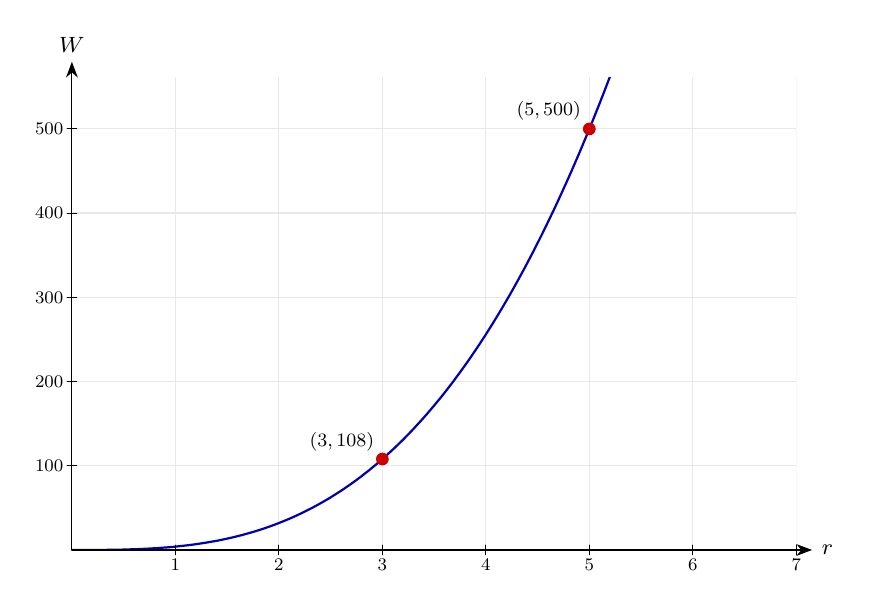
\begin{tikzpicture}[>={Stealth[length=2mm]},font=\footnotesize,line cap=round,line join=round]
\begin{scope}
\clip (0,0) rectangle (9.2,6);
\draw[gray!18] (0,0) grid[xstep=1.314,ystep=1.07] (9.2,6);
\draw[blue!70!black,thick] (0,0) -- (0.046,0) -- (0.092,0) -- (0.138,0) -- (0.184,0) -- (0.23,0) -- (0.276,0) -- (0.322,0.001) -- (0.368,0.001) -- (0.414,0.001) -- (0.46,0.002) -- (0.506,0.002) -- (0.552,0.003) -- (0.598,0.004) -- (0.644,0.005) -- (0.69,0.006) -- (0.736,0.008) -- (0.782,0.009) -- (0.828,0.011) -- (0.874,0.013) -- (0.92,0.015) -- (0.966,0.017) -- (1.012,0.02) -- (1.058,0.022) -- (1.104,0.025) -- (1.15,0.029) -- (1.196,0.032) -- (1.242,0.036) -- (1.288,0.04) -- (1.334,0.045) -- (1.38,0.05) -- (1.426,0.055) -- (1.472,0.06) -- (1.518,0.066) -- (1.564,0.072) -- (1.61,0.079) -- (1.656,0.086) -- (1.702,0.093) -- (1.748,0.101) -- (1.794,0.109) -- (1.84,0.117) -- (1.886,0.126) -- (1.932,0.136) -- (1.978,0.146) -- (2.024,0.156) -- (2.07,0.167) -- (2.116,0.179) -- (2.162,0.19) -- (2.208,0.203) -- (2.254,0.216) -- (2.3,0.229) -- (2.346,0.243) -- (2.392,0.258) -- (2.438,0.273) -- (2.484,0.289) -- (2.53,0.305) -- (2.576,0.322) -- (2.622,0.34) -- (2.668,0.358) -- (2.714,0.377) -- (2.76,0.396) -- (2.806,0.416) -- (2.852,0.437) -- (2.898,0.459) -- (2.944,0.481) -- (2.99,0.504) -- (3.036,0.527) -- (3.082,0.552) -- (3.128,0.577) -- (3.174,0.603) -- (3.22,0.629) -- (3.266,0.656) -- (3.312,0.685) -- (3.358,0.714) -- (3.404,0.743) -- (3.45,0.774) -- (3.496,0.805) -- (3.542,0.837) -- (3.588,0.87) -- (3.634,0.904) -- (3.68,0.939) -- (3.726,0.975) -- (3.772,1.011) -- (3.818,1.049) -- (3.864,1.087) -- (3.91,1.126) -- (3.956,1.167) -- (4.002,1.208) -- (4.048,1.25) -- (4.094,1.293) -- (4.14,1.337) -- (4.186,1.382) -- (4.232,1.428) -- (4.278,1.475) -- (4.324,1.523) -- (4.37,1.573) -- (4.416,1.623) -- (4.462,1.674) -- (4.508,1.726) -- (4.554,1.78) -- (4.6,1.834) -- (4.646,1.89) -- (4.692,1.946) -- (4.738,2.004) -- (4.784,2.063) -- (4.83,2.123) -- (4.876,2.185) -- (4.922,2.247) -- (4.968,2.311) -- (5.014,2.375) -- (5.06,2.441) -- (5.106,2.509) -- (5.152,2.577) -- (5.198,2.647) -- (5.244,2.717) -- (5.29,2.79) -- (5.336,2.863) -- (5.382,2.938) -- (5.428,3.014) -- (5.474,3.091) -- (5.52,3.17) -- (5.566,3.249) -- (5.612,3.331) -- (5.658,3.413) -- (5.704,3.497) -- (5.75,3.582) -- (5.796,3.669) -- (5.842,3.757) -- (5.888,3.847) -- (5.934,3.938) -- (5.98,4.03) -- (6.026,4.124) -- (6.072,4.219) -- (6.118,4.315) -- (6.164,4.413) -- (6.21,4.513) -- (6.256,4.614) -- (6.302,4.716) -- (6.348,4.82) -- (6.394,4.926) -- (6.44,5.033) -- (6.486,5.142) -- (6.532,5.252) -- (6.578,5.364) -- (6.624,5.477) -- (6.67,5.592) -- (6.716,5.708) -- (6.762,5.826) -- (6.808,5.946) -- (6.854,6.068) -- (6.9,6.191) -- (6.946,6.315) -- (6.992,6.441) -- (7.038,6.569) -- (7.084,6.699) -- (7.13,6.83) -- (7.176,6.963) -- (7.222,7.098) -- (7.268,7.235) -- (7.314,7.373) -- (7.36,7.513) -- (7.406,7.655) -- (7.452,7.798) -- (7.498,7.944) -- (7.544,8.091) -- (7.59,8.24) -- (7.636,8.39) -- (7.682,8.543) -- (7.728,8.697) -- (7.774,8.853) -- (7.82,9.012) -- (7.866,9.172) -- (7.912,9.333) -- (7.958,9.497) -- (8.004,9.663) -- (8.05,9.83) -- (8.096,10) -- (8.142,10.171) -- (8.188,10.345) -- (8.234,10.52) -- (8.28,10.697) -- (8.326,10.876) -- (8.372,11.058) -- (8.418,11.241) -- (8.464,11.426) -- (8.51,11.614) -- (8.556,11.803) -- (8.602,11.994) -- (8.648,12) -- (8.694,12) -- (8.74,12) -- (8.786,12) -- (8.832,12) -- (8.878,12) -- (8.924,12) -- (8.97,12) -- (9.016,12) -- (9.062,12) -- (9.108,12) -- (9.154,12) -- (9.2,12);
\end{scope}
\draw[->] (0,0) -- (9.4,0) node[right]{$r$};
\draw[->] (0,0) -- (0,6.2) node[above]{$W$};
\draw (1.314,-0.06) -- (1.314,0.06) node[below=2pt,scale=0.8]{$1$};
\draw (2.629,-0.06) -- (2.629,0.06) node[below=2pt,scale=0.8]{$2$};
\draw (3.943,-0.06) -- (3.943,0.06) node[below=2pt,scale=0.8]{$3$};
\draw (5.257,-0.06) -- (5.257,0.06) node[below=2pt,scale=0.8]{$4$};
\draw (6.571,-0.06) -- (6.571,0.06) node[below=2pt,scale=0.8]{$5$};
\draw (7.886,-0.06) -- (7.886,0.06) node[below=2pt,scale=0.8]{$6$};
\draw (9.2,-0.06) -- (9.2,0.06) node[below=2pt,scale=0.8]{$7$};
\draw (-0.06,1.07) -- (0.06,1.07) node[left=2pt,scale=0.8]{$100$};
\draw (-0.06,2.139) -- (0.06,2.139) node[left=2pt,scale=0.8]{$200$};
\draw (-0.06,3.209) -- (0.06,3.209) node[left=2pt,scale=0.8]{$300$};
\draw (-0.06,4.278) -- (0.06,4.278) node[left=2pt,scale=0.8]{$400$};
\draw (-0.06,5.348) -- (0.06,5.348) node[left=2pt,scale=0.8]{$500$};
\fill[red!80!black] (3.943,1.155) circle (2.3pt);
\node[above left,scale=0.85] at (3.943,1.155) {$(3,108)$};
\fill[red!80!black] (6.571,5.348) circle (2.3pt);
\node[above left,scale=0.85] at (6.571,5.348) {$(5,500)$};
\end{tikzpicture}
}
\end{center}
\small The relationship plotted, with the data points marked.\normalsize

\medskip\hrule

\section*{Proportion 47\quad\small\texttt{(cg4-047)}}
\addcontentsline{toc}{section}{Proportion 47 (cg4-047)}
\textit{Difficulty: Foundation \quad\textbar\quad Marks: 3}

\question{\( y \) is directly proportional to \( (x + 1)^2 \). When \( x = 2 \), \( y = 27 \). Find \( y \) when \( x = 4 \).}

\textbf{Worked solution.}

\textit{Step 1: Find k}
\[\begin{gathered}
y = k(x+1)^2 \implies 27 = 9k \implies k = 3
\end{gathered}\]
The whole bracket \( (x+1) \) is squared, so substitute \( x = 2 \) inside first: \( (2+1)^2 = 9 \). A common pitfall is to compute \( x^2 + 1 \) instead of \( (x+1)^2 \).

\textit{Step 2: Find y}
\[\begin{gathered}
y = 3 \times 25 = 75
\end{gathered}\]
With \( x = 4 \), the bracket is \( (4+1)^2 = 25 \). Add inside the bracket before squaring.

\begin{answerbox}
\textbf{Final answer:}\quad \(\displaystyle y = 75\)
\end{answerbox}
\textbf{Graph.}

\begin{center}
\resizebox{\ifdim\width>\linewidth \linewidth\else \width\fi}{!}{%
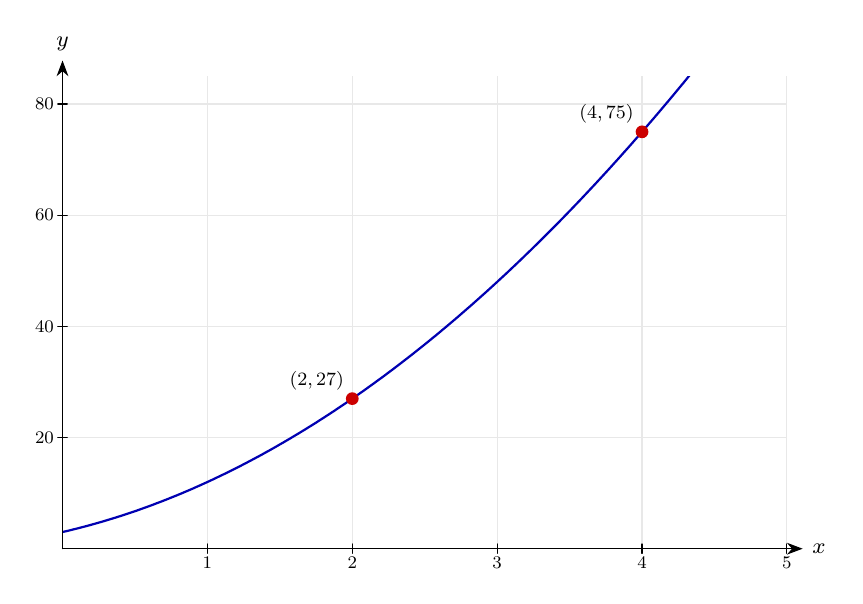
\begin{tikzpicture}[>={Stealth[length=2mm]},font=\footnotesize,line cap=round,line join=round]
\begin{scope}
\clip (0,0) rectangle (9.2,6);
\draw[gray!18] (0,0) grid[xstep=1.84,ystep=1.412] (9.2,6);
\draw[blue!70!black,thick] (0,0.212) -- (0.046,0.222) -- (0.092,0.233) -- (0.138,0.245) -- (0.184,0.256) -- (0.23,0.268) -- (0.276,0.28) -- (0.322,0.292) -- (0.368,0.305) -- (0.414,0.318) -- (0.46,0.331) -- (0.506,0.344) -- (0.552,0.358) -- (0.598,0.372) -- (0.644,0.386) -- (0.69,0.4) -- (0.736,0.415) -- (0.782,0.43) -- (0.828,0.445) -- (0.874,0.461) -- (0.92,0.476) -- (0.966,0.492) -- (1.012,0.509) -- (1.058,0.525) -- (1.104,0.542) -- (1.15,0.559) -- (1.196,0.577) -- (1.242,0.594) -- (1.288,0.612) -- (1.334,0.63) -- (1.38,0.649) -- (1.426,0.667) -- (1.472,0.686) -- (1.518,0.705) -- (1.564,0.725) -- (1.61,0.744) -- (1.656,0.764) -- (1.702,0.785) -- (1.748,0.805) -- (1.794,0.826) -- (1.84,0.847) -- (1.886,0.868) -- (1.932,0.89) -- (1.978,0.912) -- (2.024,0.934) -- (2.07,0.956) -- (2.116,0.979) -- (2.162,1.002) -- (2.208,1.025) -- (2.254,1.048) -- (2.3,1.072) -- (2.346,1.096) -- (2.392,1.12) -- (2.438,1.145) -- (2.484,1.169) -- (2.53,1.194) -- (2.576,1.22) -- (2.622,1.245) -- (2.668,1.271) -- (2.714,1.297) -- (2.76,1.324) -- (2.806,1.35) -- (2.852,1.377) -- (2.898,1.404) -- (2.944,1.432) -- (2.99,1.459) -- (3.036,1.487) -- (3.082,1.515) -- (3.128,1.544) -- (3.174,1.572) -- (3.22,1.601) -- (3.266,1.631) -- (3.312,1.66) -- (3.358,1.69) -- (3.404,1.72) -- (3.45,1.75) -- (3.496,1.781) -- (3.542,1.812) -- (3.588,1.843) -- (3.634,1.874) -- (3.68,1.906) -- (3.726,1.938) -- (3.772,1.97) -- (3.818,2.002) -- (3.864,2.035) -- (3.91,2.068) -- (3.956,2.101) -- (4.002,2.135) -- (4.048,2.168) -- (4.094,2.202) -- (4.14,2.237) -- (4.186,2.271) -- (4.232,2.306) -- (4.278,2.341) -- (4.324,2.377) -- (4.37,2.412) -- (4.416,2.448) -- (4.462,2.484) -- (4.508,2.521) -- (4.554,2.557) -- (4.6,2.594) -- (4.646,2.631) -- (4.692,2.669) -- (4.738,2.706) -- (4.784,2.744) -- (4.83,2.783) -- (4.876,2.821) -- (4.922,2.86) -- (4.968,2.899) -- (5.014,2.938) -- (5.06,2.978) -- (5.106,3.018) -- (5.152,3.058) -- (5.198,3.098) -- (5.244,3.139) -- (5.29,3.18) -- (5.336,3.221) -- (5.382,3.262) -- (5.428,3.304) -- (5.474,3.346) -- (5.52,3.388) -- (5.566,3.431) -- (5.612,3.473) -- (5.658,3.516) -- (5.704,3.56) -- (5.75,3.603) -- (5.796,3.647) -- (5.842,3.691) -- (5.888,3.736) -- (5.934,3.78) -- (5.98,3.825) -- (6.026,3.87) -- (6.072,3.916) -- (6.118,3.961) -- (6.164,4.007) -- (6.21,4.053) -- (6.256,4.1) -- (6.302,4.146) -- (6.348,4.193) -- (6.394,4.241) -- (6.44,4.288) -- (6.486,4.336) -- (6.532,4.384) -- (6.578,4.432) -- (6.624,4.481) -- (6.67,4.53) -- (6.716,4.579) -- (6.762,4.628) -- (6.808,4.678) -- (6.854,4.728) -- (6.9,4.778) -- (6.946,4.828) -- (6.992,4.879) -- (7.038,4.93) -- (7.084,4.981) -- (7.13,5.033) -- (7.176,5.084) -- (7.222,5.136) -- (7.268,5.189) -- (7.314,5.241) -- (7.36,5.294) -- (7.406,5.347) -- (7.452,5.401) -- (7.498,5.454) -- (7.544,5.508) -- (7.59,5.562) -- (7.636,5.617) -- (7.682,5.671) -- (7.728,5.726) -- (7.774,5.781) -- (7.82,5.837) -- (7.866,5.892) -- (7.912,5.948) -- (7.958,6.005) -- (8.004,6.061) -- (8.05,6.118) -- (8.096,6.175) -- (8.142,6.232) -- (8.188,6.29) -- (8.234,6.348) -- (8.28,6.406) -- (8.326,6.464) -- (8.372,6.523) -- (8.418,6.582) -- (8.464,6.641) -- (8.51,6.7) -- (8.556,6.76) -- (8.602,6.82) -- (8.648,6.88) -- (8.694,6.941) -- (8.74,7.001) -- (8.786,7.062) -- (8.832,7.124) -- (8.878,7.185) -- (8.924,7.247) -- (8.97,7.309) -- (9.016,7.372) -- (9.062,7.434) -- (9.108,7.497) -- (9.154,7.56) -- (9.2,7.624);
\end{scope}
\draw[->] (0,0) -- (9.4,0) node[right]{$x$};
\draw[->] (0,0) -- (0,6.2) node[above]{$y$};
\draw (1.84,-0.06) -- (1.84,0.06) node[below=2pt,scale=0.8]{$1$};
\draw (3.68,-0.06) -- (3.68,0.06) node[below=2pt,scale=0.8]{$2$};
\draw (5.52,-0.06) -- (5.52,0.06) node[below=2pt,scale=0.8]{$3$};
\draw (7.36,-0.06) -- (7.36,0.06) node[below=2pt,scale=0.8]{$4$};
\draw (9.2,-0.06) -- (9.2,0.06) node[below=2pt,scale=0.8]{$5$};
\draw (-0.06,1.412) -- (0.06,1.412) node[left=2pt,scale=0.8]{$20$};
\draw (-0.06,2.824) -- (0.06,2.824) node[left=2pt,scale=0.8]{$40$};
\draw (-0.06,4.235) -- (0.06,4.235) node[left=2pt,scale=0.8]{$60$};
\draw (-0.06,5.647) -- (0.06,5.647) node[left=2pt,scale=0.8]{$80$};
\fill[red!80!black] (3.68,1.906) circle (2.3pt);
\node[above left,scale=0.85] at (3.68,1.906) {$(2,27)$};
\fill[red!80!black] (7.36,5.294) circle (2.3pt);
\node[above left,scale=0.85] at (7.36,5.294) {$(4,75)$};
\end{tikzpicture}
}
\end{center}
\small The relationship plotted, with the data points marked.\normalsize

\medskip\hrule

\section*{Proportion 48\quad\small\texttt{(cg4-048)}}
\addcontentsline{toc}{section}{Proportion 48 (cg4-048)}
\textit{Difficulty: Foundation \quad\textbar\quad Marks: 3}

\question{The intensity \( I \) of light is inversely proportional to the square of the distance \( d \) from the source. At 2 m, \( I = 100 \). Find \( I \) at 5 m.}

\textbf{Worked solution.}

\textit{Step 1: Find k}
\[\begin{gathered}
I = \frac{k}{d^2} \implies 100 = \frac{k}{4} \implies k = 400
\end{gathered}\]
Inverse-square law: \( I = \frac{k}{d^2} \). Square \( d = 2 \) to get 4, then multiply both sides by 4.

\textit{Step 2: Find I}
\[\begin{gathered}
I = \frac{400}{25} = 16
\end{gathered}\]
Square \( d = 5 \) (giving 25) before dividing. Distance went up by 2.5$\times$, so \( d^2 \) went up by 6.25$\times$ and intensity dropped by the same factor (100 $\to$ 16).

\begin{answerbox}
\textbf{Final answer:}\quad \(\displaystyle I = 16\)
\end{answerbox}
\textbf{Graph.}

\begin{center}
\resizebox{\ifdim\width>\linewidth \linewidth\else \width\fi}{!}{%
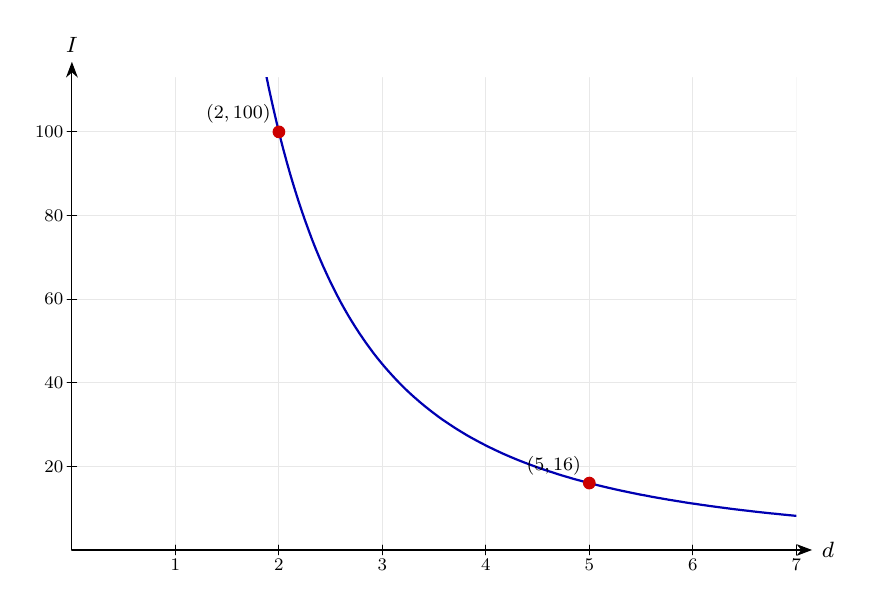
\begin{tikzpicture}[>={Stealth[length=2mm]},font=\footnotesize,line cap=round,line join=round]
\begin{scope}
\clip (0,0) rectangle (9.2,6);
\draw[gray!18] (0,0) grid[xstep=1.314,ystep=1.062] (9.2,6);
\draw[blue!70!black,thick] (0.023,12) -- (0.069,12) -- (0.115,12) -- (0.161,12) -- (0.207,12) -- (0.252,12) -- (0.298,12) -- (0.344,12) -- (0.39,12) -- (0.436,12) -- (0.482,12) -- (0.528,12) -- (0.574,12) -- (0.62,12) -- (0.665,12) -- (0.711,12) -- (0.757,12) -- (0.803,12) -- (0.849,12) -- (0.895,12) -- (0.941,12) -- (0.987,12) -- (1.032,12) -- (1.078,12) -- (1.124,12) -- (1.17,12) -- (1.216,12) -- (1.262,12) -- (1.308,12) -- (1.354,12) -- (1.4,12) -- (1.445,12) -- (1.491,12) -- (1.537,12) -- (1.583,12) -- (1.629,12) -- (1.675,12) -- (1.721,12) -- (1.767,11.755) -- (1.813,11.167) -- (1.858,10.623) -- (1.904,10.117) -- (1.95,9.646) -- (1.996,9.208) -- (2.042,8.799) -- (2.088,8.416) -- (2.134,8.058) -- (2.18,7.723) -- (2.225,7.407) -- (2.271,7.111) -- (2.317,6.832) -- (2.363,6.57) -- (2.409,6.322) -- (2.455,6.088) -- (2.501,5.866) -- (2.547,5.657) -- (2.593,5.458) -- (2.638,5.27) -- (2.684,5.091) -- (2.73,4.922) -- (2.776,4.76) -- (2.822,4.607) -- (2.868,4.461) -- (2.914,4.321) -- (2.96,4.188) -- (3.006,4.061) -- (3.051,3.94) -- (3.097,3.824) -- (3.143,3.713) -- (3.189,3.607) -- (3.235,3.506) -- (3.281,3.408) -- (3.327,3.315) -- (3.373,3.225) -- (3.418,3.139) -- (3.464,3.057) -- (3.51,2.977) -- (3.556,2.901) -- (3.602,2.828) -- (3.648,2.757) -- (3.694,2.689) -- (3.74,2.623) -- (3.786,2.56) -- (3.831,2.499) -- (3.877,2.44) -- (3.923,2.384) -- (3.969,2.329) -- (4.015,2.276) -- (4.061,2.225) -- (4.107,2.175) -- (4.153,2.127) -- (4.199,2.081) -- (4.244,2.036) -- (4.29,1.993) -- (4.336,1.951) -- (4.382,1.911) -- (4.428,1.871) -- (4.474,1.833) -- (4.52,1.796) -- (4.566,1.76) -- (4.612,1.725) -- (4.657,1.691) -- (4.703,1.658) -- (4.749,1.627) -- (4.795,1.596) -- (4.841,1.566) -- (4.887,1.536) -- (4.933,1.508) -- (4.979,1.48) -- (5.024,1.453) -- (5.07,1.427) -- (5.116,1.402) -- (5.162,1.377) -- (5.208,1.353) -- (5.254,1.329) -- (5.3,1.306) -- (5.346,1.284) -- (5.392,1.262) -- (5.437,1.241) -- (5.483,1.22) -- (5.529,1.2) -- (5.575,1.18) -- (5.621,1.161) -- (5.667,1.142) -- (5.713,1.124) -- (5.759,1.106) -- (5.805,1.089) -- (5.85,1.072) -- (5.896,1.055) -- (5.942,1.039) -- (5.988,1.023) -- (6.034,1.008) -- (6.08,0.993) -- (6.126,0.978) -- (6.172,0.963) -- (6.217,0.949) -- (6.263,0.935) -- (6.309,0.922) -- (6.355,0.908) -- (6.401,0.895) -- (6.447,0.883) -- (6.493,0.87) -- (6.539,0.858) -- (6.585,0.846) -- (6.63,0.835) -- (6.676,0.823) -- (6.722,0.812) -- (6.768,0.801) -- (6.814,0.79) -- (6.86,0.78) -- (6.906,0.769) -- (6.952,0.759) -- (6.998,0.749) -- (7.043,0.74) -- (7.089,0.73) -- (7.135,0.721) -- (7.181,0.711) -- (7.227,0.702) -- (7.273,0.694) -- (7.319,0.685) -- (7.365,0.676) -- (7.41,0.668) -- (7.456,0.66) -- (7.502,0.652) -- (7.548,0.644) -- (7.594,0.636) -- (7.64,0.629) -- (7.686,0.621) -- (7.732,0.614) -- (7.778,0.606) -- (7.823,0.599) -- (7.869,0.592) -- (7.915,0.586) -- (7.961,0.579) -- (8.007,0.572) -- (8.053,0.566) -- (8.099,0.559) -- (8.145,0.553) -- (8.191,0.547) -- (8.236,0.541) -- (8.282,0.535) -- (8.328,0.529) -- (8.374,0.523) -- (8.42,0.517) -- (8.466,0.512) -- (8.512,0.506) -- (8.558,0.501) -- (8.603,0.496) -- (8.649,0.49) -- (8.695,0.485) -- (8.741,0.48) -- (8.787,0.475) -- (8.833,0.47) -- (8.879,0.465) -- (8.925,0.461) -- (8.971,0.456) -- (9.016,0.451) -- (9.062,0.447) -- (9.108,0.442) -- (9.154,0.438) -- (9.2,0.433);
\end{scope}
\draw[->] (0,0) -- (9.4,0) node[right]{$d$};
\draw[->] (0,0) -- (0,6.2) node[above]{$I$};
\draw (1.314,-0.06) -- (1.314,0.06) node[below=2pt,scale=0.8]{$1$};
\draw (2.629,-0.06) -- (2.629,0.06) node[below=2pt,scale=0.8]{$2$};
\draw (3.943,-0.06) -- (3.943,0.06) node[below=2pt,scale=0.8]{$3$};
\draw (5.257,-0.06) -- (5.257,0.06) node[below=2pt,scale=0.8]{$4$};
\draw (6.571,-0.06) -- (6.571,0.06) node[below=2pt,scale=0.8]{$5$};
\draw (7.886,-0.06) -- (7.886,0.06) node[below=2pt,scale=0.8]{$6$};
\draw (9.2,-0.06) -- (9.2,0.06) node[below=2pt,scale=0.8]{$7$};
\draw (-0.06,1.062) -- (0.06,1.062) node[left=2pt,scale=0.8]{$20$};
\draw (-0.06,2.124) -- (0.06,2.124) node[left=2pt,scale=0.8]{$40$};
\draw (-0.06,3.186) -- (0.06,3.186) node[left=2pt,scale=0.8]{$60$};
\draw (-0.06,4.248) -- (0.06,4.248) node[left=2pt,scale=0.8]{$80$};
\draw (-0.06,5.31) -- (0.06,5.31) node[left=2pt,scale=0.8]{$100$};
\fill[red!80!black] (2.629,5.31) circle (2.3pt);
\node[above left,scale=0.85] at (2.629,5.31) {$(2,100)$};
\fill[red!80!black] (6.571,0.85) circle (2.3pt);
\node[above left,scale=0.85] at (6.571,0.85) {$(5,16)$};
\end{tikzpicture}
}
\end{center}
\small The relationship plotted, with the data points marked.\normalsize

\medskip\hrule

\section*{Proportion 49\quad\small\texttt{(cg4-049)}}
\addcontentsline{toc}{section}{Proportion 49 (cg4-049)}
\textit{Difficulty: Foundation \quad\textbar\quad Marks: 4}

\question{Given \( y = \frac{k}{x} \) and \( y = 8 \) when \( x = 3 \), find the value of \( x \) when \( y = x \).}

\textbf{Worked solution.}

\textit{Step 1: Find k}
\[\begin{gathered}
8 = \frac{k}{3} \implies k = 24
\end{gathered}\]
Substitute the known pair into \( y = \frac{k}{x} \) and multiply both sides by 3 to isolate \( k \).

\textit{Step 2: Set y = x}
\[\begin{gathered}
x = \frac{24}{x} \implies x^2 = 24 \implies x = \sqrt{24} = 2\sqrt{6}
\end{gathered}\]
Replace \( y \) with \( x \), then multiply both sides by \( x \) to clear the fraction. Simplify the surd: \( \sqrt{24} = \sqrt{4 \times 6} = 2\sqrt{6} \); reject the negative root since the original equation \( x = 24/x \) requires \( x \) and \( 24/x \) to share a sign.

\begin{answerbox}
\textbf{Final answer:}\quad \(\displaystyle x = 2\sqrt{6}\)
\end{answerbox}
\textbf{Graph.}

\begin{center}
\resizebox{\ifdim\width>\linewidth \linewidth\else \width\fi}{!}{%
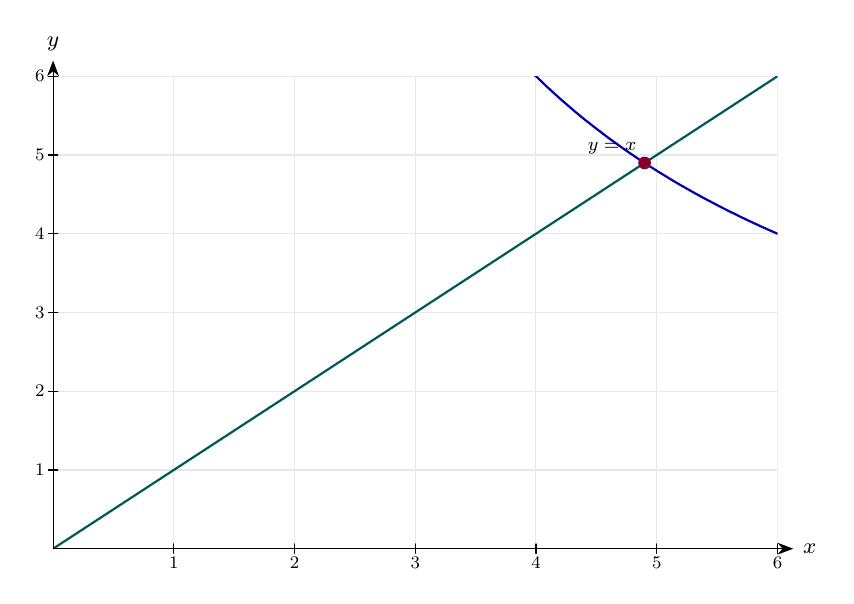
\begin{tikzpicture}[>={Stealth[length=2mm]},font=\footnotesize,line cap=round,line join=round]
\begin{scope}
\clip (0,0) rectangle (9.2,6);
\draw[gray!18] (0,0) grid[xstep=1.533,ystep=1] (9.2,6);
\draw[teal!70!black,thick] (0,0) -- (9.2,6);
\draw[blue!70!black,thick] (0.023,12) -- (0.069,12) -- (0.115,12) -- (0.161,12) -- (0.207,12) -- (0.252,12) -- (0.298,12) -- (0.344,12) -- (0.39,12) -- (0.436,12) -- (0.482,12) -- (0.528,12) -- (0.574,12) -- (0.62,12) -- (0.665,12) -- (0.711,12) -- (0.757,12) -- (0.803,12) -- (0.849,12) -- (0.895,12) -- (0.941,12) -- (0.987,12) -- (1.032,12) -- (1.078,12) -- (1.124,12) -- (1.17,12) -- (1.216,12) -- (1.262,12) -- (1.308,12) -- (1.354,12) -- (1.4,12) -- (1.445,12) -- (1.491,12) -- (1.537,12) -- (1.583,12) -- (1.629,12) -- (1.675,12) -- (1.721,12) -- (1.767,12) -- (1.813,12) -- (1.858,12) -- (1.904,12) -- (1.95,12) -- (1.996,12) -- (2.042,12) -- (2.088,12) -- (2.134,12) -- (2.18,12) -- (2.225,12) -- (2.271,12) -- (2.317,12) -- (2.363,12) -- (2.409,12) -- (2.455,12) -- (2.501,12) -- (2.547,12) -- (2.593,12) -- (2.638,12) -- (2.684,12) -- (2.73,12) -- (2.776,12) -- (2.822,12) -- (2.868,12) -- (2.914,12) -- (2.96,12) -- (3.006,12) -- (3.051,12) -- (3.097,11.881) -- (3.143,11.708) -- (3.189,11.539) -- (3.235,11.376) -- (3.281,11.217) -- (3.327,11.062) -- (3.373,10.911) -- (3.418,10.765) -- (3.464,10.622) -- (3.51,10.484) -- (3.556,10.348) -- (3.602,10.216) -- (3.648,10.088) -- (3.694,9.963) -- (3.74,9.84) -- (3.786,9.721) -- (3.831,9.605) -- (3.877,9.491) -- (3.923,9.38) -- (3.969,9.272) -- (4.015,9.166) -- (4.061,9.062) -- (4.107,8.961) -- (4.153,8.862) -- (4.199,8.765) -- (4.244,8.67) -- (4.29,8.577) -- (4.336,8.487) -- (4.382,8.398) -- (4.428,8.311) -- (4.474,8.226) -- (4.52,8.142) -- (4.566,8.06) -- (4.612,7.98) -- (4.657,7.901) -- (4.703,7.824) -- (4.749,7.749) -- (4.795,7.675) -- (4.841,7.602) -- (4.887,7.53) -- (4.933,7.46) -- (4.979,7.392) -- (5.024,7.324) -- (5.07,7.258) -- (5.116,7.193) -- (5.162,7.129) -- (5.208,7.066) -- (5.254,7.004) -- (5.3,6.944) -- (5.346,6.884) -- (5.392,6.826) -- (5.437,6.768) -- (5.483,6.711) -- (5.529,6.656) -- (5.575,6.601) -- (5.621,6.547) -- (5.667,6.494) -- (5.713,6.442) -- (5.759,6.39) -- (5.805,6.34) -- (5.85,6.29) -- (5.896,6.241) -- (5.942,6.193) -- (5.988,6.146) -- (6.034,6.099) -- (6.08,6.053) -- (6.126,6.007) -- (6.172,5.963) -- (6.217,5.919) -- (6.263,5.875) -- (6.309,5.833) -- (6.355,5.791) -- (6.401,5.749) -- (6.447,5.708) -- (6.493,5.668) -- (6.539,5.628) -- (6.585,5.589) -- (6.63,5.55) -- (6.676,5.512) -- (6.722,5.474) -- (6.768,5.437) -- (6.814,5.401) -- (6.86,5.365) -- (6.906,5.329) -- (6.952,5.294) -- (6.998,5.259) -- (7.043,5.225) -- (7.089,5.191) -- (7.135,5.158) -- (7.181,5.125) -- (7.227,5.092) -- (7.273,5.06) -- (7.319,5.028) -- (7.365,4.997) -- (7.41,4.966) -- (7.456,4.935) -- (7.502,4.905) -- (7.548,4.875) -- (7.594,4.846) -- (7.64,4.817) -- (7.686,4.788) -- (7.732,4.76) -- (7.778,4.732) -- (7.823,4.704) -- (7.869,4.676) -- (7.915,4.649) -- (7.961,4.622) -- (8.007,4.596) -- (8.053,4.57) -- (8.099,4.544) -- (8.145,4.518) -- (8.191,4.493) -- (8.236,4.468) -- (8.282,4.443) -- (8.328,4.419) -- (8.374,4.395) -- (8.42,4.371) -- (8.466,4.347) -- (8.512,4.323) -- (8.558,4.3) -- (8.603,4.277) -- (8.649,4.255) -- (8.695,4.232) -- (8.741,4.21) -- (8.787,4.188) -- (8.833,4.166) -- (8.879,4.145) -- (8.925,4.123) -- (8.971,4.102) -- (9.016,4.081) -- (9.062,4.061) -- (9.108,4.04) -- (9.154,4.02) -- (9.2,4);
\end{scope}
\draw[->] (0,0) -- (9.4,0) node[right]{$x$};
\draw[->] (0,0) -- (0,6.2) node[above]{$y$};
\draw (1.533,-0.06) -- (1.533,0.06) node[below=2pt,scale=0.8]{$1$};
\draw (3.067,-0.06) -- (3.067,0.06) node[below=2pt,scale=0.8]{$2$};
\draw (4.6,-0.06) -- (4.6,0.06) node[below=2pt,scale=0.8]{$3$};
\draw (6.133,-0.06) -- (6.133,0.06) node[below=2pt,scale=0.8]{$4$};
\draw (7.667,-0.06) -- (7.667,0.06) node[below=2pt,scale=0.8]{$5$};
\draw (9.2,-0.06) -- (9.2,0.06) node[below=2pt,scale=0.8]{$6$};
\draw (-0.06,1) -- (0.06,1) node[left=2pt,scale=0.8]{$1$};
\draw (-0.06,2) -- (0.06,2) node[left=2pt,scale=0.8]{$2$};
\draw (-0.06,3) -- (0.06,3) node[left=2pt,scale=0.8]{$3$};
\draw (-0.06,4) -- (0.06,4) node[left=2pt,scale=0.8]{$4$};
\draw (-0.06,5) -- (0.06,5) node[left=2pt,scale=0.8]{$5$};
\draw (-0.06,6) -- (0.06,6) node[left=2pt,scale=0.8]{$6$};
\fill[purple!70!black] (7.512,4.899) circle (2.3pt);
\node[above left,scale=0.85] at (7.512,4.899) {$y=x$};
\end{tikzpicture}
}
\end{center}
\small The relationship plotted, with the data points marked.\normalsize

\medskip\hrule

\section*{Proportion 50\quad\small\texttt{(cg4-050)}}
\addcontentsline{toc}{section}{Proportion 50 (cg4-050)}
\textit{Difficulty: Foundation \quad\textbar\quad Marks: 3}

\question{\( y \) is proportional to \( x^n \). When \( x \) is tripled, \( y \) is multiplied by 9. Find \( n \).}

\textbf{Worked solution.}

\textit{Step 1: Set up}
\[\begin{gathered}
y = kx^n; \quad k(3x)^n = 9kx^n \implies 3^n = 9
\end{gathered}\]
Write the original relation, then replace \( x \) with \( 3x \). The new \( y \) is \( 9 \) times the old, so divide both sides by \( kx^n \) --- the constants cancel, leaving \( 3^n \) on its own.

\textit{Step 2: Solve}
\[\begin{gathered}
3^n = 3^2 \implies n = 2
\end{gathered}\]
Write 9 as \( 3^2 \). With matching bases, the exponents must be equal, so \( n = 2 \).

\begin{answerbox}
\textbf{Final answer:}\quad \(\displaystyle n = 2\)
\end{answerbox}
\textbf{Graph.}

\begin{center}
\resizebox{\ifdim\width>\linewidth \linewidth\else \width\fi}{!}{%
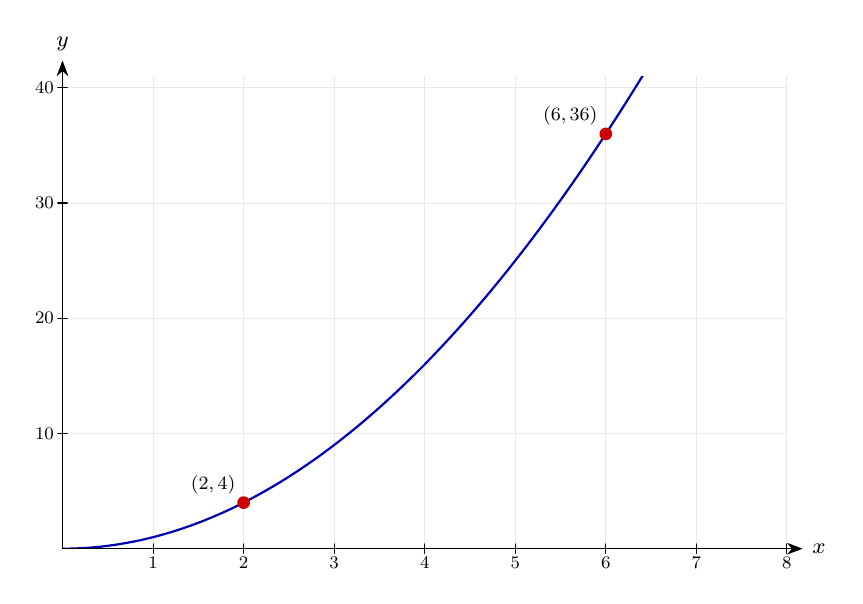
\begin{tikzpicture}[>={Stealth[length=2mm]},font=\footnotesize,line cap=round,line join=round]
\begin{scope}
\clip (0,0) rectangle (9.2,6);
\draw[gray!18] (0,0) grid[xstep=1.15,ystep=1.463] (9.2,6);
\draw[blue!70!black,thick] (0,0) -- (0.046,0) -- (0.092,0.001) -- (0.138,0.002) -- (0.184,0.004) -- (0.23,0.006) -- (0.276,0.008) -- (0.322,0.011) -- (0.368,0.015) -- (0.414,0.019) -- (0.46,0.023) -- (0.506,0.028) -- (0.552,0.034) -- (0.598,0.04) -- (0.644,0.046) -- (0.69,0.053) -- (0.736,0.06) -- (0.782,0.068) -- (0.828,0.076) -- (0.874,0.085) -- (0.92,0.094) -- (0.966,0.103) -- (1.012,0.113) -- (1.058,0.124) -- (1.104,0.135) -- (1.15,0.146) -- (1.196,0.158) -- (1.242,0.171) -- (1.288,0.184) -- (1.334,0.197) -- (1.38,0.211) -- (1.426,0.225) -- (1.472,0.24) -- (1.518,0.255) -- (1.564,0.271) -- (1.61,0.287) -- (1.656,0.303) -- (1.702,0.321) -- (1.748,0.338) -- (1.794,0.356) -- (1.84,0.375) -- (1.886,0.394) -- (1.932,0.413) -- (1.978,0.433) -- (2.024,0.453) -- (2.07,0.474) -- (2.116,0.495) -- (2.162,0.517) -- (2.208,0.539) -- (2.254,0.562) -- (2.3,0.585) -- (2.346,0.609) -- (2.392,0.633) -- (2.438,0.658) -- (2.484,0.683) -- (2.53,0.708) -- (2.576,0.734) -- (2.622,0.761) -- (2.668,0.788) -- (2.714,0.815) -- (2.76,0.843) -- (2.806,0.871) -- (2.852,0.9) -- (2.898,0.929) -- (2.944,0.959) -- (2.99,0.989) -- (3.036,1.02) -- (3.082,1.051) -- (3.128,1.083) -- (3.174,1.115) -- (3.22,1.147) -- (3.266,1.18) -- (3.312,1.214) -- (3.358,1.248) -- (3.404,1.282) -- (3.45,1.317) -- (3.496,1.352) -- (3.542,1.388) -- (3.588,1.425) -- (3.634,1.461) -- (3.68,1.499) -- (3.726,1.536) -- (3.772,1.574) -- (3.818,1.613) -- (3.864,1.652) -- (3.91,1.692) -- (3.956,1.732) -- (4.002,1.772) -- (4.048,1.813) -- (4.094,1.855) -- (4.14,1.897) -- (4.186,1.939) -- (4.232,1.982) -- (4.278,2.025) -- (4.324,2.069) -- (4.37,2.113) -- (4.416,2.158) -- (4.462,2.203) -- (4.508,2.249) -- (4.554,2.295) -- (4.6,2.341) -- (4.646,2.389) -- (4.692,2.436) -- (4.738,2.484) -- (4.784,2.533) -- (4.83,2.581) -- (4.876,2.631) -- (4.922,2.681) -- (4.968,2.731) -- (5.014,2.782) -- (5.06,2.833) -- (5.106,2.885) -- (5.152,2.937) -- (5.198,2.99) -- (5.244,3.043) -- (5.29,3.097) -- (5.336,3.151) -- (5.382,3.205) -- (5.428,3.26) -- (5.474,3.316) -- (5.52,3.372) -- (5.566,3.428) -- (5.612,3.485) -- (5.658,3.542) -- (5.704,3.6) -- (5.75,3.659) -- (5.796,3.717) -- (5.842,3.777) -- (5.888,3.836) -- (5.934,3.896) -- (5.98,3.957) -- (6.026,4.018) -- (6.072,4.08) -- (6.118,4.142) -- (6.164,4.204) -- (6.21,4.267) -- (6.256,4.331) -- (6.302,4.395) -- (6.348,4.459) -- (6.394,4.524) -- (6.44,4.589) -- (6.486,4.655) -- (6.532,4.721) -- (6.578,4.788) -- (6.624,4.855) -- (6.67,4.923) -- (6.716,4.991) -- (6.762,5.06) -- (6.808,5.129) -- (6.854,5.198) -- (6.9,5.268) -- (6.946,5.339) -- (6.992,5.41) -- (7.038,5.481) -- (7.084,5.553) -- (7.13,5.625) -- (7.176,5.698) -- (7.222,5.771) -- (7.268,5.845) -- (7.314,5.919) -- (7.36,5.994) -- (7.406,6.069) -- (7.452,6.145) -- (7.498,6.221) -- (7.544,6.298) -- (7.59,6.375) -- (7.636,6.452) -- (7.682,6.53) -- (7.728,6.609) -- (7.774,6.687) -- (7.82,6.767) -- (7.866,6.847) -- (7.912,6.927) -- (7.958,7.008) -- (8.004,7.089) -- (8.05,7.171) -- (8.096,7.253) -- (8.142,7.336) -- (8.188,7.419) -- (8.234,7.502) -- (8.28,7.586) -- (8.326,7.671) -- (8.372,7.756) -- (8.418,7.841) -- (8.464,7.927) -- (8.51,8.014) -- (8.556,8.101) -- (8.602,8.188) -- (8.648,8.276) -- (8.694,8.364) -- (8.74,8.453) -- (8.786,8.542) -- (8.832,8.632) -- (8.878,8.722) -- (8.924,8.812) -- (8.97,8.903) -- (9.016,8.995) -- (9.062,9.087) -- (9.108,9.179) -- (9.154,9.272) -- (9.2,9.366);
\end{scope}
\draw[->] (0,0) -- (9.4,0) node[right]{$x$};
\draw[->] (0,0) -- (0,6.2) node[above]{$y$};
\draw (1.15,-0.06) -- (1.15,0.06) node[below=2pt,scale=0.8]{$1$};
\draw (2.3,-0.06) -- (2.3,0.06) node[below=2pt,scale=0.8]{$2$};
\draw (3.45,-0.06) -- (3.45,0.06) node[below=2pt,scale=0.8]{$3$};
\draw (4.6,-0.06) -- (4.6,0.06) node[below=2pt,scale=0.8]{$4$};
\draw (5.75,-0.06) -- (5.75,0.06) node[below=2pt,scale=0.8]{$5$};
\draw (6.9,-0.06) -- (6.9,0.06) node[below=2pt,scale=0.8]{$6$};
\draw (8.05,-0.06) -- (8.05,0.06) node[below=2pt,scale=0.8]{$7$};
\draw (9.2,-0.06) -- (9.2,0.06) node[below=2pt,scale=0.8]{$8$};
\draw (-0.06,1.463) -- (0.06,1.463) node[left=2pt,scale=0.8]{$10$};
\draw (-0.06,2.927) -- (0.06,2.927) node[left=2pt,scale=0.8]{$20$};
\draw (-0.06,4.39) -- (0.06,4.39) node[left=2pt,scale=0.8]{$30$};
\draw (-0.06,5.854) -- (0.06,5.854) node[left=2pt,scale=0.8]{$40$};
\fill[red!80!black] (2.3,0.585) circle (2.3pt);
\node[above left,scale=0.85] at (2.3,0.585) {$(2,4)$};
\fill[red!80!black] (6.9,5.268) circle (2.3pt);
\node[above left,scale=0.85] at (6.9,5.268) {$(6,36)$};
\end{tikzpicture}
}
\end{center}
\small The relationship plotted, with the data points marked.\normalsize

\medskip\hrule

\end{document}
